\documentclass[12pt]{book}

\usepackage[utf8]{inputenc}

\usepackage[spanish,es-tabla]{babel}

\usepackage{geometry}
\geometry{margin=2.5cm}

\usepackage{amsmath,amssymb,amsthm,amsfonts}
\usepackage{bm}
\usepackage{centernot}

\usepackage{graphicx}
\usepackage{tikz}
\usepackage{tkz-graph}
\usetikzlibrary{graphs,graphs.standard,arrows.meta,bending,positioning,arrows,shapes,babel}

\usepackage{multicol}
\usepackage{enumitem}

\usepackage{xcolor}
\usepackage{color}

\usepackage[most]{tcolorbox}
\tcbuselibrary{theorems, breakable}

\usepackage{booktabs}
%\usepackage{proof}

\usepackage{float}
\usepackage{wrapfig}
\usepackage{ifthen}

\usepackage{hyperref}

\definecolor{OliveGreen}{rgb}{0,0.6,0}
\definecolor{Maroon}{rgb}{0.5,0,0}
\definecolor{fuchsia}{rgb}{1.0, 0.0, 1.0}

\newcommand{\blue}[1] {\textcolor{blue}{ #1} }
\newcommand{\red}[1] {\textcolor{red}{ #1} }
\newcommand{\green}[1] {\textcolor{green}{ #1} }
\newcommand{\brown}[1] {\textcolor{brown}{ #1} }
\newcommand{\fuchsia}[1] {\textcolor{fuchsia}{ #1} }
\newcommand{\white}[1] {\textcolor{white}{ #1} }
\newcommand{\grey}[1] {\textcolor{gray}{ #1} }



%rules of inference
\usepackage{fancybox}
\newcommand{\Rule}[2]{\genfrac{}{}{0.7pt}{}{{\setlength{\fboxrule}{0pt}\setlength{\fboxsep}{3mm}\fbox{$#1$}}}{{\setlength{\fboxrule}{0pt}\setlength{\fboxsep}{3mm}\fbox{$#2$}}}}

\newcommand{\Rulee}[3]{\genfrac{}{}{0.7pt}{}{{\setlength{\fboxrule}{0pt}\setlength{\fboxsep}{3mm}\fbox{$#1$}}}{{\setlength{\fboxrule}{0pt}\setlength{\fboxsep}{3mm}\fbox{$#2$}}}[#3]}


\newenvironment{thmblock}[1]{%
    \tcbset{colframe=yellow!50!black, colback=lightgray!10, coltitle=black, fonttitle=\bfseries}%
    \begin{tcolorbox}[title=#1]%
}{%
    \end{tcolorbox}%
}
% colframe=blue!60, colback=blue!5

% colframe=lightgray!80!black, colback=lightgray!10
\newenvironment{definitionblock}[1]{%
    \begin{tcolorbox}[
        colframe=red!60,
        colback=red!5, 
        coltitle=black,
        fonttitle=\bfseries,
        title=#1
    ]%
}{%
    \end{tcolorbox}%
}

\newenvironment{exampleblock}[1]{%
    \begin{tcolorbox}[
        colframe=lightgray!80!black,
        colback=lightgray!10,
        fonttitle=\bfseries,
        title=#1
    ]%
}{%
    \end{tcolorbox}%
}


\makeatletter
\renewenvironment{proof}[1][Demostración]{%
  \par\pushQED{\qed}%
  \normalfont\topsep6pt \trivlist\item[\hskip\labelsep
    \color{blue!70!black}\bfseries #1.]\ignorespaces
}{%
  \popQED\endtrivlist\@endpefalse
}
\makeatother


\newcommand{\alert}[1]{\textbf{#1}}
\newcommand{\impblock}[1]{\textbf{#1}}
\newcommand{\stitle}[1]{\textit{#1}}

\newcommand{\perm}[2]{\mathsf{P}\left(#1,#2\right)}
\newcommand{\comb}[2]{\mathsf{C}\left(#1,#2\right)}

\newcommand{\nat}{\mathbb{N}}
\renewcommand{\int}{\mathbb{Z}}
\newcommand{\real}{\mathbb{R}}


\newcommand{\newboxquestion}[1]{\noindent \textbf{#1}} 


\newcommand{\degin}[1]{\mathit{deg^{in}}\left(#1\right)}
\newcommand{\degout}[1]{\mathit{deg^{out}}\left(#1\right)}

\setlength{\parskip}{4pt} % Espacio de 10 puntos entre párrafos


\newif\ifshowsolutions
% \showsolutionstrue % cambiar a \showsolutionsfalse para ocultar soluciones
\showsolutionsfalse



\begin{document}

\begin{titlepage}
  % \vspace*{2cm}
  \begin{minipage}{0.4\textwidth}
    
\includegraphics[width=\linewidth]{dcc_2019_cuadrado_blanco.png}
  \end{minipage}
  \hfill
  \begin{minipage}{0.6\textwidth}
    \centering
    % {\scshape\Large Universidad de Chile \par}
    % {\scshape\Large Departamento de Ciencias de la Computación \par}
  \end{minipage}

  \vspace{3cm}

  \begin{center}
    {\Huge\bfseries Apuntes de Matemáticas Discretas para la Computación \par}
    \vspace{2cm}
    {\Large Andrés Abeliuk \par}
    \vspace{1cm}
     {\large 2025 \par}
  \end{center}

  \vfill

  \begin{center}
    \small
    Este apunte han sido elaborado a partir de las diapositivas del curso CC3101, Matemáticas Discretas, impartido por el DCC de la Universidad de Chile por Alejandro Hevia, Federico Olmedo y Jocelyn Simmonds.
  \end{center}
\end{titlepage}




\setcounter{tocdepth}{1}  % Solo mostrar hasta \section en el índice
% \maketitle
\let\cleardoublepage\relax
\let\clearpage\relax
\tableofcontents
\newpage

\part{Fundamentos de La Lógica}
\chapter{Lógica Proposicional}



\section{¿Qué es la lógica?}


La lógica es una disciplina fundamental para el razonamiento y la estructura del conocimiento. Se centra en determinar cuándo un argumento es válido, es decir, en la relación entre premisas y conclusión, sin importar el contenido específico de las afirmaciones.

\subsection{Breve Historia de la Lógica}

La lógica ha experimentado una evolución  a lo largo de la historia. Desde sus inicios en la antigua Grecia hasta su aplicación en la computación moderna, la lógica ha dejado una huella en diversas áreas del saber.

Todo comenzó con \textbf{Aristóteles} en el siglo IV a.C., quien estableció los cimientos de la lógica formal al introducir el silogismo. Este método de razonamiento deductivo, basado en premisas y conclusiones, sentó las bases para el desarrollo de sistemas lógicos más complejos.

Siglos después, la \textbf{lógica estoica} (siglos III a.C.-II d.C.) emergió con un enfoque innovador. Los estoicos desarrollaron un sistema lógico basado en operadores y reglas inferenciales, anticipando ideas esenciales que hoy son pilares de la lógica contemporánea.

Avanzando en el tiempo, \textbf{George Boole} (1815-1864) revolucionó el campo con su lógica booleana. Este sistema algebraico para el razonamiento lógico no solo transformó la lógica, sino que también sentó las bases para la computación moderna.

\textbf{Gottlob Frege} (1848-1925) llevó la lógica a otro nivel al introducir el cálculo de predicados y la cuantificación lógica. Estos conceptos se convirtieron en fundamentos esenciales para la computación, las matemáticas y la filosofía analítica.

Finalmente, \textbf{Claude Shannon} (1937) aplicó la lógica booleana a circuitos eléctricos en su tesis de maestría, \textit{A Symbolic Analysis of Relay and Switching Circuits}. Este trabajo seminal marcó el inicio de la era de la computación digital, demostrando cómo la lógica puede ser utilizada para diseñar y optimizar sistemas electrónicos.

Estos hitos históricos ilustran cómo la lógica ha evolucionado y se ha adaptado, proporcionando herramientas poderosas para el razonamiento y la innovación en diversas disciplinas.

\subsection{Aplicaciones de la Lógica en Ciencias de la Computación}

La lógica, en sus diversas formas, es una herramienta esencial en el campo de las ciencias de la computación. En el diseño de \textbf{lenguajes de programación}, la lógica formal proporciona las bases para definir sintaxis y semántica, asegurando que los programas sean coherentes y funcionales. 

En la \textbf{verificación de software}, la lógica garantiza que los programas cumplan con sus especificaciones, detectando errores y mejorando la calidad del código. Las \textbf{bases de datos y los motores de búsqueda} también se benefician de la lógica, permitiendo la formulación de consultas eficientes y la extracción de información relevante de grandes volúmenes de datos.

La lógica se utiliza en \textbf{ciberseguridad y criptografía} para analizar protocolos y detectar vulnerabilidades, asegurando la integridad y confidencialidad de la información. Además, en el desarrollo de \textbf{algoritmos y estructuras de datos}, la lógica proporciona un marco riguroso para diseñar soluciones eficientes y optimizadas. Finalmente,en la utilizainteligencia artificial se utiliza para modelar el razonamiento y la toma de decisiones, permitiendo la creación de sistemas autónomos y adaptativos. 

En todos estos ámbitos, la lógica proporciona un marco riguroso para estructurar el conocimiento y alcanzar conclusiones fundamentadas.



\subsection{Tipos de Lógica}

El razonamiento formal se apoya en diversos sistemas lógicos, cada uno con su propia expresividad y aplicaciones. A continuación, se presentan algunos de los más importantes.

La \textbf{lógica proposicional} es fundamental para el razonamiento lógico, utilizando proposiciones atómicas y conectivos lógicos para formar expresiones complejas. Se enfoca en las relaciones entre proposiciones y es esencial en matemáticas, computación y sistemas formales.

La \textbf{lógica de primer orden, o lógica de predicados}, amplía la lógica proposicional al introducir cuantificadores y predicados, permitiendo afirmaciones más detalladas sobre objetos en un dominio. Es más expresiva y se usa ampliamente en matemáticas, filosofía y ciencias de la computación.

La \textbf{lógica modal} introduce operadores para razonar sobre modalidades como la posibilidad y la necesidad, permitiendo considerar lo que es verdadero en diferentes contextos. Tiene aplicaciones en filosofía, inteligencia artificial y teoría de la información. La \textbf{lógica temporal} es una extension con operadores temporales para expresar conceptos como ``siempre'', ``eventualmente'' y ``hasta que'', lo que  permite modelar procesos dinámicos.

En este curso, nos centraremos en la \textbf{lógica proposicional y de primer orden}, Estos sistemas son la base para construir modelos más avanzados de inferencia y representación del conocimiento.


\section{Razonamiento Formal}
La l\'ogica proposicional es una de las formas m\'as fundamentales de razonamiento formal, proporcionando una base estructurada para la inferencia y el análisis lógico de argumentos.


\subsection{Definiciones B\'asicas}

\begin{itemize}
    \item Una \textbf{proposici\'on} es cualquier enunciado que puede ser verdadero o falso, pero no ambos simult\'aneamente.
    \item Un \textbf{argumento} es una secuencia de proposiciones donde las primeras se llaman premisas y la \'ultima se llama conclusi\'on.
    \item Un argumento es \textbf{v\'alido} si la verdad de sus premisas garantiza la verdad de su conclusi\'on.
\end{itemize}


\subsection{Argumentos}

Un \textbf{argumento} es una secuencia de proposiciones que se estructuran de manera tal que una o más premisas conducen a una conclusión. Aristóteles fue pionero en el estudio de los argumentos, desarrollando la teoría del silogismo para analizar patrones lógicos de razonamiento.

Un ejemplo clásico de silogismo es el siguiente:

\begin{center}
\begin{tabular}{l}
Todas las personas son mortales.  \\
Sócrates es una persona.  \\
\cline{1-1}
Por lo tanto, Sócrates es mortal. 
\end{tabular}
\end{center}

Este es un ejemplo de \textit{razonamiento deductivo}, donde la conclusión se deduce necesariamente de las premisas. La validez del silogismo reside en que, si las premisas son verdaderas, la conclusión debe serlo también.
En este caso, la inferencia se basa en el hecho de que todas las personas comparten la propiedad de ser mortales, y Sócrates pertenece a este grupo.

\subsection{Validez de un Argumento}
La \textbf{validez} de un argumento se refiere a la relación lógica entre las premisas y la conclusión. Un argumento es válido si, bajo la suposición de que todas sus premisas son verdaderas, la conclusión también debe ser necesariamente verdadera. Es decir, un argumento válido garantiza que no es posible que las premisas sean verdaderas y la conclusión falsa al mismo tiempo.

Por ejemplo, consideremos el siguiente argumento:

\begin{center}
\begin{tabular}{l}
Todas las especies de aves pueden volar. \\
Un pingüino es un ave. \\
\cline{1-1}
Por lo tanto, un pingüino puede volar. 
\end{tabular}
\end{center}

Aunque la primera premisa es falsa, la estructura lógica del argumento sigue siendo válida, ya que la conclusión se deriva formalmente de las premisas. Es importante resaltar que la validez no implica que las premisas sean realmente ciertas en el mundo real, sino que la inferencia es correcta desde un punto de vista lógico.\\

\begin{tcolorbox}[colback=yellow!20, colframe=black, sharp corners=south]
Un argumento \textbf{válido} es aquel en el que, si todas las premisas son verdaderas, la conclusión necesariamente también lo es. Esto garantiza que no puede haber un caso en el que las premisas sean verdaderas y la conclusión falsa.
\end{tcolorbox}

\bigskip

\textbf{Ejemplo de argumento válido:}
\begin{center}
\begin{tabular}{l}
Si llueve, entonces el suelo estará mojado. \\
Está lloviendo. \\
\cline{1-1}
Por lo tanto, el suelo está mojado.
\end{tabular}
\end{center}


Un argumento tiene una \textbf{forma lógica}, es decir, una representación simbólica que abstrae su estructura subyacente mediante variables y conectores lógicos. En esta representación, las proposiciones se representan con letras (por ejemplo, $p$, $q$, $r$) y los conectores lógicos (como $\rightarrow$ para implicación, $\vee$ para disyunción, $\wedge$ para conjunción, y $\lnot$ para negación) se utilizan para mostrar las relaciones entre las proposiciones.


El argumento anterior tiene la siguiente forma lógica:
\begin{center}
\begin{tabular}{l}
$p \rightarrow q$ \\
$p$ \\
\hline
$q$
\end{tabular}
\end{center}


Este razonamiento sigue la estructura del \textit{modus ponens}, una regla de inferencia fundamental en lógica proposicional. Dado que la primera premisa establece una implicación (``si llueve, entonces el suelo estará mojado'') y la segunda premisa afirma la verdad de su antecedente (``está lloviendo''), la conclusión (``el suelo está mojado'') se sigue necesariamente.\\

En contraste, un \textbf{argumento inválido} es aquel en el que, aunque las premisas sean verdaderas, la conclusión no necesariamente lo es. 

\textbf{Ejemplo de argumento inválido:}
\begin{center}
\begin{tabular}{l}
Si llueve, entonces el suelo estará mojado. \\
El suelo está mojado. \\
\cline{1-1}
Por lo tanto, está lloviendo.
\end{tabular}
\end{center}

Este argumento es inválido porque, aunque la premisa ``el suelo está mojado'' sea verdadera, existen otras posibles causas para que el suelo esté mojado, como el riego de un jardín. Por lo tanto, la conclusión ``está lloviendo'' no necesariamente se sigue de las premisas.

Comprender la distinción entre un argumento válido e inválido es fundamental para el análisis lógico. Un argumento válido garantiza que, si las premisas son verdaderas, la conclusión también será verdadera, pero no asegura la verdad de las premisas. La validez, por lo tanto, se refiere únicamente a la relación lógica entre las premisas y la conclusión, no a la veracidad de las afirmaciones contenidas en las premisas.

\subsection{Ejemplos de Argumentos y su Forma Lógica}

En esta sección analizaremos diferentes tipos de argumentos y su representación lógica.
Los argumentos en los \textbf{ejemplos 1 y 2} pueden expresarse utilizando únicamente \textbf{proposiciones atómicas} y \textbf{conectivos lógicos}.
El argumento en el \textbf{ejemplo 3} requiere una lógica más expresiva, incorporando \textbf{predicados} y \textbf{cuantificadores}.



\subsubsection{Ejemplo 1: Argumento válido}
\textbf{Argumento:}

\begin{center}
\begin{tabular}{l}
Si Ana estudia en el DCC o en el DIM, entonces tomará CC3101.\\
Ana estudia en el DCC.\\
\hline
Por lo tanto, Ana tomará CC3101.
\end{tabular}
\end{center}

\textbf{Forma lógica:}

\begin{center}
\begin{tabular}{l}
$(p \vee q) \rightarrow r$ \\
$p$ \\
\hline
$r$
\end{tabular}
\end{center}

\textbf{Análisis:} Este argumento es válido porque la conclusión se sigue necesariamente de las premisas. La estructura lógica muestra que si Ana estudia en el DCC ($p$), entonces tomará CC3101 ($r$).

\subsubsection{Ejemplo 2: Argumento no válido}
\textbf{Argumento:}

\begin{center}
\begin{tabular}{l}
Si llueve, entonces se moja el suelo.\\
No llovió.\\
\hline
Por lo tanto, no se mojó el suelo.
\end{tabular}
\end{center}

\textbf{Forma lógica:}

\begin{center}
\begin{tabular}{l}
$p \rightarrow q$ \\
$\lnot p$ \\
\hline
$\lnot q$
\end{tabular}
\end{center}

\textbf{Análisis:} 
Este argumento comete la \textbf{falacia de la negación del antecedente}, ya que de \( p \rightarrow q \) y \( \lnot p \) no se sigue necesariamente \( \lnot q \). La implicación solo garantiza que si \( p \) ocurre, entonces \( q \) también; sin embargo, \( q \) podría darse por otras razones. En este caso, el suelo podría mojarse de otra forma (por ejemplo, con una manguera), por lo que la conclusión no es válida.  








\subsubsection{Ejemplo 3: Argumento válido}
\textbf{Argumento:}

\begin{center}
\begin{tabular}{l}
Todas las personas son mortales.\\
Sócrates es una persona.\\
\hline
Por lo tanto, Sócrates es mortal.
\end{tabular}
\end{center}

\textbf{Forma lógica:}

\begin{center}
\begin{tabular}{l}
$\forall x.~~\mathit{persona}(x) \rightarrow \mathit{mortal}(x)$ \\
$\mathit{persona}(\mathsf{Socrates})$ \\
\hline
$ \mathit{mortal}(\mathsf{Socrates})$
\end{tabular}
\end{center}

\textbf{Análisis:} Este argumento es válido porque la conclusión se sigue necesariamente de las premisas. La estructura lógica muestra que si Sócrates es una persona ($\mathit{persona}(\mathsf{Socrates})$), entonces Sócrates es mortal ($\mathit{mortal}(\mathsf{Socrates})$).




% \newpage



\section{Lógica Proposicional}

La lógica proposicional es el punto de partida en el estudio del razonamiento lógico. Este enfoque se centra en las \textbf{proposiciones}, que son enunciados que pueden ser verdaderos o falsos, pero no ambos simultáneamente.

Una \textbf{proposición} es cualquier enunciado que puede ser evaluado como verdadero o falso. Por ejemplo, las siguientes son proposiciones:
\begin{itemize}
    \item Ana estudia en el DCC.
    \item Santiago es la capital de Chile.
    \item $2 > 4$.
\end{itemize}
En contraste, las siguientes no son proposiciones porque no pueden ser evaluadas como verdaderas o falsas:
\begin{itemize}
    \item ¿Qué hora es?
    \item $x == 2$.
\end{itemize}

La validez de un argumento en la lógica proposicional puede ser determinada mediante dos métodos principales: \textbf{tablas de verdad} y \textbf{sistemas de inferencia}. Las tablas de verdad permiten evaluar todas las combinaciones posibles de valores de verdad para las proposiciones involucradas, mientras que los sistemas de inferencia proporcionan reglas para derivar nuevas proposiciones a partir de las conocidas.

\subsection{Sintaxis}

La sintaxis en lógica proposicional define las reglas que determinan cuándo una secuencia de símbolos constituye una \textbf{fórmula bien formada}. 

La sintaxis es fundamental porque establece las reglas que deben seguirse para construir expresiones lógicas válidas. Estas reglas aseguran que las proposiciones sean claras y sin ambigüedades, lo cual es crucial para el razonamiento lógico.

\bigskip

\begin{tabular}{ll}
    \stitle{Fórmulas bien formadas:} & $p \land q$, $\lnot p \rightarrow p$, $q$ \\
    \stitle{Fórmulas no bien formadas:} & $p\: \land$, $q\; p\; \lnot\; p$, $\lor$ \\
\end{tabular}

\subsubsection{Conjunto de Fórmulas Bien Formadas}

Una fórmula bien formada es o bien una \textbf{fórmula atómica}, formada por una proposición, o bien una \textbf{fórmula compuesta}, formada combinando proposiciones a través de conectivos lógicos.

\bigskip

\begin{thmblock}{Definición (sintaxis de la lógica proposicional)}
    Dado un conjunto $P=\{p,q,r,\ldots\}$ de proposiciones, el conjunto de \textbf{fórmulas bien formadas} sobre $P$, notado \textbf{$\mathcal{L}(P)$}, se define inductivamente de la siguiente manera:\\

    \textbf{Caso base:} Si $p \in P$, entonces $p \in \mathcal{L}(P)$. \\
    \textbf{Caso inductivo:} Si $\alpha,\beta \in \mathcal{L}(P)$, entonces $(\lnot \alpha)$, $(\alpha \land \beta)$, $(\alpha \lor \beta)$, $(\alpha \rightarrow \beta) \in \mathcal{L}(P)$.
\end{thmblock}

% \subsubsection{Supresión de Paréntesis}

Para evitar el aglutinamiento de paréntesis en las fórmulas nos permitimos omitir el par de paréntesis más externos e introducimos un orden de precedencia sobre los conectivos lógicos: $\lnot$, $\land$, $\lor$, $\rightarrow$.

\bigskip

\stitle{Ejemplo:}

\begin{center}
    \begin{tabular}{@{} lr @{}}
        \toprule
        Fórmula & Forma Abreviada\\
        \midrule
        $( (\lnot p) \rightarrow q)$ & $\lnot p \rightarrow q$ \\
        $((p \land q) \lor r)$ & $p \land q \lor r$\\
        \bottomrule
    \end{tabular}
\end{center}



\subsection{Semántica}

% \subsubsection{Objetivo de la Semántica}

La semántica de un lenguaje lógico define las reglas que permiten determinar cuándo una fórmula bien formada es verdadera o falsa. Es decir, establece el significado preciso de las expresiones del lenguaje y cómo su veracidad depende de los valores asignados a sus componentes.

Una herramienta clave en esta definición es la \textbf{función de verdad}, que asigna a cada combinación de valores de las proposiciones atómicas un valor de verdad para la fórmula completa:

\[
\textbf{Función de verdad: }\{0,1\}^n \rightarrow \{0,1\}
\]

El valor de verdad de una fórmula $\alpha \in \mathcal{L}(P)$ depende únicamente del valor de verdad de las proposiciones en $\mathcal{L}(P)$ y del significado de los conectivos lógicos, dado por su \alert{tabla de verdad}.

\bigskip

Para ilustrar, consideremos la fórmula $\alpha = p \land q$. Su tabla de verdad es:
\begin{center}
\begin{tabular}{c|c|c}
    $p$ & $q$ & $p \land q$ \\
    \hline
    V & V & V \\
    V & F & F \\
    F & V & F \\
    F & F & F \\
\end{tabular}
\end{center}

\bigskip

La función de verdad asigna un valor de verdad (0 para falso, 1 para verdadero) a cada combinación de valores de verdad de las proposiciones atómicas. Esto se realiza mediante la tabla de verdad correspondiente a la fórmula $\alpha$.

% \bigskip

% La semántica es esencial porque permite evaluar la validez de los argumentos lógicos. Al asignar valores de verdad a las proposiciones atómicas y utilizar las tablas de verdad, podemos verificar si un argumento es válido. Esto asegura que nuestros razonamientos sean coherentes y basados en principios lógicos sólidos.

% \bigskip

% En resumen, la semántica proporciona las herramientas necesarias para interpretar y evaluar las fórmulas lógicas, garantizando que nuestros argumentos sean consistentes y válidos.




\subsubsection{Tabla de Verdad de la Negación ($\neg$)}

\begin{center}
    \begin{tabular}{|c||c|}
        \hline
        $\alpha$ & $\neg \alpha$ \\
        \hline
        1 & 0 \\
        \hline
        0 & 1 \\
        \hline
    \end{tabular}
\end{center}

\impblock{El valor de verdad de $\lnot \alpha$ es opuesto al de $\alpha$.}

\subsubsection{Tabla de Verdad de la Conjunción ($\land$)}

\begin{center}
    \begin{tabular}{|c|c||c|}
        \hline
        $\alpha$ & $\beta$ & $\alpha \land \beta$ \\
        \hline
        1 & 1 & 1 \\
        \hline
        1 & 0 & 0 \\
        \hline
        0 & 1 & 0 \\
        \hline
        0 & 0 & 0 \\
        \hline
    \end{tabular}
\end{center}

\impblock{$\alpha \land \beta$ es verdadero si y sólo si $\alpha$ y $\beta$ son verdaderos.}

\subsubsection{Tabla de Verdad de la Disyunción ($\lor$)}

\begin{center}
    \begin{tabular}{|c|c||c|}
        \hline
        $\alpha$ & $\beta$ & $\alpha \lor \beta$ \\
        \hline
        1 & 1 & 1 \\
        \hline
        1 & 0 & 1 \\
        \hline
        0 & 1 & 1 \\
        \hline
        0 & 0 & 0 \\
        \hline
    \end{tabular}
\end{center}

\impblock{$\alpha \lor \beta$ es verdadero si y sólo si $\alpha$ o $\beta$ son verdaderos.}

\subsubsection{Tabla de Verdad de la Implicancia ($\rightarrow$)}

\begin{center}
    \begin{tabular}{|c|c||c|}
        \hline
        $\alpha$ & $\beta$ & $\alpha \rightarrow \beta$ \\
        \hline
        1 & 1 & 1 \\
        \hline
        1 & 0 & 0 \\
        \hline
        0 & 1 & 1 \\
        \hline
        0 & 0 & 1 \\
        \hline
    \end{tabular}
\end{center}

\impblock{$\alpha \rightarrow \beta$ es siempre verdadero, excepto cuando $\alpha$ (el antecedente) es verdadero y $\beta$ (el consecuente) es falso.}

\subsubsection{Valor de Verdad de Fórmulas Compuestas}

El valor de verdad de una fórmula lógica compuesta se determina a partir de los valores de verdad de sus proposiciones atómicas y de las reglas establecidas por los conectivos lógicos.  

\bigskip

\paragraph{Ejemplo:} Determinar el valor de verdad de la siguiente fórmula para cada valuación de las proposiciones \( p \) y \( q \):  

\[
(p \lor q) \rightarrow (p \land q)
\]

\bigskip

\begin{center}
    \begin{tabular}{|c|c||c|c|c|}
        \hline
        \( p \) & \( q \) & \( p \lor q \) & \( p \land q \) & \( (p \lor q) \rightarrow (p \land q) \) \\
        \hline
        1 & 1 & 1 & 1 & 1 \\
        1 & 0 & 1 & 0 & 0 \\
        0 & 1 & 1 & 0 & 0 \\
        0 & 0 & 0 & 0 & 1 \\
        \hline
    \end{tabular}
\end{center}

\bigskip

En la tabla de verdad anterior, se observa cómo el valor de la fórmula se obtiene paso a paso aplicando las definiciones de los conectivos lógicos. Esto nos permite verificar su comportamiento en todas las posibles valuaciones de \( p \) y \( q \).


\subsubsection{Semántica de la Lógica Proposicional}

Alternativamente, podemos formalizar lo anterior de la siguiente manera:

\begin{thmblock}{Definición (semántica de la lógica proposicional)}
    Sea $$\sigma \colon P \rightarrow \{0,1\}$$ una \alert{valuación} de las proposiciones en $P=\{p,q,r,\ldots\}$, es decir una función que le asigna un valor de verdad a las proposiciones en $P$.

    La función $$\hat{\sigma} \colon \mathcal{L}(P) \rightarrow \{0,1\}$$ le asigna un valor de verdad a cada fórmula en $\mathcal{L}(P)$ de la siguiente manera:
    $$
    \begin{array}{l c l}
        \hat{\sigma}(p) &=& \sigma(p) \quad \text{para } p \in P\\
        \hat{\sigma}(\lnot \alpha) &=& 1 - \hat{\sigma}(\alpha) \\
        \hat{\sigma}(\alpha \land \beta) &=& \min\,\{\hat{\sigma}(\alpha), \hat{\sigma}(\beta) \} \\
        \hat{\sigma}(\alpha \lor \beta) &=& \max\,\{\hat{\sigma}(\alpha), \hat{\sigma}(\beta) \} \\
        \hat{\sigma}(\alpha \rightarrow \beta) &=& \max\,\{1-\hat{\sigma}(\alpha), \hat{\sigma}(\beta) \}
    \end{array}
    $$
\end{thmblock}

\subsection{Definición Formal de un Argumento Válido}

Un \textbf{argumento} es válido si y solo si, dado un conjunto de premisas \( P_1, P_2, \dots, P_n \) y una conclusión \( C \), siempre que todas las premisas sean verdaderas, la conclusión también debe ser verdadera. Formalmente, esto se expresa de la siguiente manera:

\[
(P_1 \land P_2 \land \dots \land P_n) \rightarrow C
\]

Es decir, un argumento \( \langle P_1, P_2, \dots, P_n, C \rangle \) es válido si y solo si, en cualquier interpretación donde todas las premisas \( P_1, P_2, \dots, P_n \) sean verdaderas, la conclusión \( C \) también es verdadera. Si existe una interpretación en la que todas las premisas sean verdaderas y la conclusión falsa, entonces el argumento no es válido.

\subsubsection{Ejemplos}

\bigskip

\textbf{Ejemplo 1: Modus Ponens}  

\begin{center}
\begin{tabular}{l}
$p \rightarrow q$ \\
$p$ \\
\hline
$q$
\end{tabular}
\end{center}

Para determinar la validez de este argumento, construimos su tabla de verdad:

\begin{center}
\begin{tabular}{|c|c|c|c|}
\hline
$p$ & $q$ & $p \rightarrow q$ & $q$ \\
\hline
1 & 1 & 1 & 1 \\
1 & 0 & 0 & 0 \\
0 & 1 & 1 & 1 \\
0 & 0 & 1 & 0 \\
\hline
\end{tabular}
\end{center}

En este caso, observamos que siempre que \( p \) es verdadero y \( p \rightarrow q \) también es verdadero, \( q \) debe ser verdadero. Por lo tanto, el argumento es válido.


\bigskip  

\textbf{Ejemplo 2: Silogismo Hipotético}  

Consideremos el siguiente argumento:

\begin{center}
\begin{tabular}{l}
$p \rightarrow q$ \\
$q \rightarrow r$ \\
\hline
$p \rightarrow r$
\end{tabular}
\end{center}

Para determinar si este argumento es válido, construimos su tabla de verdad:

\begin{center}
\begin{tabular}{|c|c|c|c|c|c|c|}
\hline
$p$ & $q$ & $r$ & $p \rightarrow q$ & $q \rightarrow r$ & $p \rightarrow r$ \\
\hline
1 & 1 & 1 & 1 & 1 & 1 \\
1 & 1 & 0 & 1 & 0 & 0 \\
1 & 0 & 1 & 0 & 1 & 1 \\
1 & 0 & 0 & 0 & 1 & 0 \\
0 & 1 & 1 & 1 & 1 & 1 \\
0 & 1 & 0 & 1 & 0 & 1 \\
0 & 0 & 1 & 1 & 1 & 1 \\
0 & 0 & 0 & 1 & 1 & 1 \\
\hline
\end{tabular}
\end{center}

En la tabla de verdad, observamos que, en todas las filas en las que tanto \( p \rightarrow q \) como \( q \rightarrow r \) son verdaderos, \( p \rightarrow r \) también es verdadero. Esto significa que siempre que las premisas son verdaderas, la conclusión también es verdadera. Por lo tanto, el argumento es válido.


Este tipo de razonamiento, conocido como \textbf{Silogismo Hipotético} se basa en la propiedad transitiva de las implicaciones en la lógica proposicional.



\bigskip  


\textbf{Ejemplo 3: Argumento No Válido}

Considere el siguiente argumento:

\begin{center}
\begin{tabular}{l}
$p \rightarrow r$ \\
$\lnot p$ \\
\hline
$\lnot r$
\end{tabular}
\end{center}


Para determinar si este argumento es válido, construimos su tabla de verdad:

\begin{center}
\begin{tabular}{|c|c|c|c|c|}
\hline
$p$ & $r$ & $p \rightarrow r$ & $\lnot p$ & $\lnot r$ \\
\hline
1 & 1 & 1 & 0 & 0 \\
1 & 0 & 0 & 0 & 1 \\
0 & 1 & 1 & 1 & 0 \\
0 & 0 & 1 & 1 & 1 \\
\hline
\end{tabular}
\end{center}

En este caso, observamos que en la tercera fila, donde \( p \) es falso, \( p \rightarrow r \) es verdadero, y \( \lnot p \) es verdadero, pero la conclusión \( \lnot r \) es falsa. Esto muestra que es posible que todas las premisas sean verdaderas mientras que la conclusión sea falsa. Por lo tanto, este argumento no es válido.

\bigskip

En resumen, un argumento es válido si y solo si, en todas las interpretaciones donde las premisas son verdaderas, la conclusión también lo es. Si existe una interpretación en la que las premisas sean verdaderas y la conclusión falsa, entonces el argumento no es válido.
\section{Clasificación de Fórmulas en Lógica Proposicional}

En esta sección, estudiaremos cómo se pueden clasificar distintas fórmulas de la lógica proposicional según sus propiedades lógicas. Esto nos permitirá entender mejor la estructura de los enunciados lógicos y su comportamiento bajo distintas valuaciones.

\subsection{Satisfactibilidad}

En lógica proposicional, una de las propiedades fundamentales de un conjunto de fórmulas es su \textbf{satisfactibilidad}. Esta propiedad nos indica si existe al menos una asignación de valores de verdad a las variables proposicionales que haga verdaderas todas las fórmulas de un conjunto dado.

\begin{thmblock}{Definición: Satisfactibilidad}
  Un conjunto de fórmulas \( \Gamma = \{\alpha, \beta, \gamma, \ldots\} \subseteq \mathcal{L}(P) \) se dice \textbf{satisfactible} si y solo si existe al menos una valuación \( \sigma \colon P \to \{0,1\} \) tal que:
  \[
    \hat{\sigma}(\alpha) = \hat{\sigma}(\beta) = \hat{\sigma}(\gamma) = \dots = 1.
  \]
  En caso contrario, si no existe ninguna valuación que haga verdaderas todas las fórmulas del conjunto simultáneamente, se dice que \( \Gamma \) es \textbf{insatisfactible}.
\end{thmblock}

\subsubsection*{Ejemplos de Satisfactibilidad e Insatisfactibilidad}

Para comprender mejor esta definición, consideremos algunos ejemplos concretos:

\begin{itemize}
  \item \( \{p \lor q\} \) es un conjunto satisfactible, ya que, por ejemplo, la valuación \( \sigma(p) = 1, \sigma(q) = 0 \) hace que la fórmula sea verdadera.
  \item \( \{p \land q, p \land \lnot q\} \) es insatisfactible, porque no hay una valuación que pueda hacer ambas fórmulas verdaderas al mismo tiempo. En efecto, la primera exige que \( p \) y \( q \) sean verdaderos, mientras que la segunda requiere que \( p \) sea verdadero pero \( q \) sea falso, lo cual es contradictorio.
\end{itemize}

\subsubsection*{Aplicaciones de la Satisfactibilidad}

El problema de satisfactibilidad proposicional (SAT) fue el primero en demostrarse \textbf{NP-completo} (Teorema de Cook, 1971). Ser NP-completo implica que la resolución de SAT en su forma general puede requerir un tiempo exponencial en función del número de variables, lo que hace que su solución sea computacionalmente difícil a gran escala. in embargo, en la práctica, existen algoritmos avanzados llamados \textbf{SAT-solvers} que pueden resolver muchas instancias grandes de manera eficiente mediante heurísticas y optimización.

Tiene múltiples aplicaciones en diversas áreas de la informática y la matemática:

\begin{itemize}
  \item \textbf{Verificación de software y hardware:} Se utiliza en la verificación formal de circuitos digitales y programas para determinar si existen errores lógicos en su funcionamiento. 

  \item \textbf{Optimización combinatoria:} La satisfactibilidad booleana es la base de problemas de optimización como el problema del corte mínimo, la asignación de tareas y la generación de horarios.

\item \textbf{Criptografía y seguridad informática:} Problemas SAT se usan en el análisis de protocolos criptográficos para detectar vulnerabilidades. También se aplican en la recuperación de claves cifradas y en la verificación de la resistencia de sistemas de seguridad.


\end{itemize}



\subsection{Tautologías y Contradicciones}

Otra clasificación importante en lógica proposicional es la de \textbf{tautologías} y \textbf{contradicciones}. Estas nociones permiten identificar fórmulas que son siempre verdaderas o siempre falsas, independientemente de la valuación que se elija.

\begin{thmblock}{Definición: Tautología y Contradicción}
  Una fórmula \( \alpha \in \mathcal{L}(P) \) es una \textbf{tautología} si y solo si es verdadera bajo \emph{todas} las valuaciones posibles, es decir, si para toda valuación \( \sigma \colon P \to \{0,1\} \) se cumple que:
  \[
    \hat{\sigma}(\alpha) = 1.
  \]
  
  Una fórmula \( \alpha \in \mathcal{L}(P) \) es una \textbf{contradicción} si y solo si es falsa bajo \emph{todas} las valuaciones posibles, es decir, si para toda valuación \( \sigma \colon P \to \{0,1\} \) se cumple que:
  \[
    \hat{\sigma}(\alpha) = 0.
  \]
\end{thmblock}

\subsubsection*{Ejemplos de Tautologías y Contradicciones}

A continuación, se presentan algunos ejemplos para ilustrar estas definiciones:


  \begin{itemize}
    \item \( p \lor \lnot p \) es una tautología, ya que siempre será verdadera sin importar la valuación de \( p \).
    \item \( p \rightarrow (p \lor q) \) es también una tautología, pues siempre que \( p \) sea verdadero, entonces $p \lor q$ también lo será.
    \item \( p \land \lnot p \) es una contradicción, ya que nunca puede ser verdadera, sin importar la valuación de \( p \).
  \end{itemize}


\subsection{Relación entre Contradicción e Insatisfactibilidad}

Una contradicción es una fórmula que es falsa bajo todas las valuaciones posibles. Por lo tanto, un conjunto que contenga al menos una contradicción es insatisfactible, ya que no existe ninguna valuación que lo haga verdadero.

De manera más general, un conjunto de fórmulas es insatisfactible cuando la conjunción de todas sus fórmulas forma una contradicción. Esto significa que no hay una asignación de valores de verdad que satisfaga simultáneamente todas las fórmulas del conjunto.

\begin{exampleblock}{Ejemplo} 
  El conjunto \( \{p \lor q, \lnot p, \lnot q\} \) es insatisfactible, ya que su conjunción equivale a la contradicción \( (p \lor q) \land \lnot p \land \lnot q \), la cual es falsa bajo cualquier valuación.
\end{exampleblock}


\section{Equivalencia de fórmulas}

Comprender la equivalencia de fórmulas es útil para la simplificación de expresiones lógicas y la verificación de argumentos. Nos permite transformar fórmulas en formas más manejables y demostrar propiedades de los sistemas lógicos.

Informalmente, dos fórmulas $\alpha,\beta \in \mathcal{L}(P)$ se dicen \textbf{equivalentes} si tienen la misma tabla de verdad. Formalmente:

\begin{thmblock}{Definición: Equivalencia}
Dos fórmulas $\alpha,\beta \in \mathcal{L}(P)$ son (semánticamente) \textbf{equivalentes}, notado $\alpha \equiv \beta$, si y sólo si $$ \hat{\sigma}(\alpha) = \hat{\sigma}(\beta)$$ para toda valuación $\sigma \colon P \rightarrow \{0,1\}$.
\end{thmblock}

\subsubsection*{Ejemplo}

Demostremos que $\lnot(p \lor q) \equiv \lnot p \land \lnot q$ mediante su tabla de verdad.

\begin{center} 
\begin{tabular}{|c|c||c|c|}
\hline 
p & q  &  $\lnot(p \lor q)$ & $ \lnot p \land \lnot q $ \\\hline 
1 &  1 &   0  &  0 \\\hline 
1 & 0 &  0  & 0  \\\hline 
0 & 1 &  0  & 0  \\\hline 
0 & 0 &  1  & 1  \\\hline 
\end{tabular}
\end{center}

Se observa que ambas columnas son iguales, por lo que las fórmulas son equivalentes.

\subsection{Algunas equivalencias útiles}

Las siguientes equivalencias son herramientas esenciales en la manipulación de expresiones lógicas:

\begin{thmblock}{Equivalencias útiles}
\begin{align*}     
\text{Leyes de De Morgan} \quad & \neg (p \wedge q)  \equiv  \neg p \vee \neg q \\
& \neg (p \vee q)  \equiv  \neg p \wedge \neg q \\
\\
\text{Asociatividad de } \wedge \text{ y } \vee \quad & p \wedge (q \wedge r)  \equiv  (p \wedge q) \wedge r\\
& p \vee (q \vee r) \equiv (p \vee q) \vee r\\
\\
\text{Caracterización alternativa de } \rightarrow \quad & p \rightarrow q  \equiv  \neg p \vee q
\end{align*}
\end{thmblock}

\begin{exampleblock}{Ejercicio de Equivalencia}
\begin{center}
\textbf{¿Es el conectivo de implicación  ($\rightarrow$) asociativo?}
\end{center}
Para responder esta pregunta, basta con analizar la equivalencia:
\[
(p \rightarrow q ) \rightarrow r  \equiv   p \rightarrow (q  \rightarrow r ) 
\]
Que podemos verificar si son iguales usando las tablas de verdad.
\end{exampleblock}


%%%%%%%%%%%%%%%%%%%%%%%%%%%
\section{Consecuencia Lógica}

La noción de \textbf{consecuencia lógica} es clave en lógica matemática, ya que permite formalizar cuándo una \textbf{conclusión} se \textbf{deriva} lógicamente de un \textbf{conjunto de premisas}. Esta noción subyace en el concepto de inferencia lógica y es clave para la validez de argumentos.

Sea $\Gamma$ un conjunto de fórmulas (premisas) y $\alpha$ una fórmula (conclusión). Decimos que $\alpha$ es \textbf{consecuencia lógica} de $\Gamma$ si cada vez que todas las fórmulas en $\Gamma$ son verdaderas, entonces $\alpha$ también es verdadera. Escribimos esto como:
\[ \Gamma \models \alpha. \]

Es decir, si asumimos que las premisas son verdaderas, entonces la conclusión necesariamente también debe serlo. Si encontramos al menos una interpretación en la que todas las premisas son verdaderas y la conclusión es falsa, entonces no hay consecuencia lógica.

En lógica, la \textbf{validez} es una propiedad que tienen los argumentos cuando las premisas implican la conclusión. Si la conclusión es una consecuencia lógica de las premisas, se dice que el argumento es \textbf{deductivamente válido}. En este contexto, consideraremos estas dos nociones como idénticas.


\subsection{Ejemplos Clásicos de Consecuencia Lógica}

Existen reglas clásicas de inferencia que ejemplifican el concepto de consecuencia lógica. Algunas de ellas son:

\begin{itemize}
    \item \textbf{Modus ponens}: \quad $\{p, p \rightarrow q\} \models q$
    \item \textbf{Modus tollens}: \quad $\{\neg q, p \rightarrow q\} \models \neg p$
    \item \textbf{Transitividad de la implicación}: \quad $\{p \rightarrow q, q \rightarrow r\} \models p \rightarrow r$
\end{itemize}

Estos esquemas de inferencia pueden verificarse mediante tablas de verdad como lo hicimos al verificar si un argumento es valido.


\subsection{Definición Formal}

\begin{thmblock}{Definición: Consecuencia lógica} Sea $\Gamma$ un conjunto de fórmulas en un lenguaje lógico $\mathcal{L}(P)$ y $\alpha$ una fórmula en el mismo lenguaje. Decimos que $\alpha$ es \textbf{consecuencia lógica} de $\Gamma$, denotado $\Gamma \models \alpha$, si y sólo si para toda valuación $\sigma : P \to \{0,1\}$,
\[ \text{si } \hat{\sigma}(\Gamma) = 1, \text{ entonces } \hat{\sigma}(\alpha) = 1. \]

Esto significa que $\alpha$ debe ser verdadero en toda valuación en la que todas las fórmulas de $\Gamma$ son verdaderas.
\end{thmblock}

Notar que no nos importan aquellas valuaciones $\sigma$ donde $\hat{\sigma}(\Gamma) \neq 1$. El valor de $\alpha$  en esas valuaciones es irrelevante.

\subsection{Propiedades Importantes}

La consecuencia lógica cumple con varias propiedades fundamentales que nos permiten derivar resultados de manera más estructurada y comprender mejor las relaciones entre distintas proposiciones. A continuación, presentamos algunas propiedades relevantes:


Para todo conjunto de fórmulas $\Gamma$ y todas las fórmulas $\alpha, \beta$ se cumplen las siguientes propiedades:

\begin{itemize}
    \item \textbf{Equivalencia lógica:} $\alpha \equiv \beta$ si y sólo si $\{\alpha\} \models \beta$ y $\{\beta\} \models \alpha$. Esto significa que ambas fórmulas tienen el mismo valor de verdad en todas las interpretaciones.
    
    \item \textbf{Relación con insatisfactibilidad:} $\Gamma \models \alpha$ si y sólo si $\Gamma \cup \{\neg \alpha\}$ es insatisfactible. Esta propiedad es útil para demostrar la validez de inferencias mediante el método de reducción al absurdo.
    
    \item \textbf{Regla de deducción:} $\Gamma \models \alpha \rightarrow \beta$ si y sólo si $\Gamma \cup \{\alpha\} \models \beta$. Es un recurso esencial para derivar conclusiones en sistemas formales.
    
    \item \textbf{Monotonía:} Si $\Gamma \models \alpha$ entonces $\Gamma \cup \{ \beta \} \models \alpha$. Esto significa que al agregar más premisas a $\Gamma$, no se pierde la capacidad de inferir $\alpha$.
\end{itemize}

\subsubsection*{Ejemplo de Monotonía con un Conjunto Insatisfactible}

\noindent\textbf{Pregunta:}\; Sabemos que $\{p,\ p \rightarrow q\} \models q$. Por la propiedad de monotonía de la consecuencia lógica, también se cumple:
\[
\{p,\ p \rightarrow q,\ \neg q\} \models q.
\]
\textbf{\emph{¿Cómo es esto posible?}}

La respuesta radica en que $\{p, p \rightarrow q, \neg q\}$ es un conjunto \emph{insatisfactible}; no existe valuación que haga todas estas fórmulas verdaderas simultáneamente. En lógica proposicional, cuando un conjunto de premisas es insatisfactible, se sigue trivialmente que se puede derivar cualquier conclusión.

\begin{itemize}
\item Si un conjunto es insatisfactible, no hay asignaciones de verdad que satisfagan simultáneamente todas sus fórmulas.
\item Por definición, en cada valuación que ``satisface'' el conjunto (no existe ninguna), la conclusión es verdadera de manera vacía o trivial.
\end{itemize}

Este hecho, aunque pueda parecer extraño, se desprende directamente de nuestras definiciones y pone de manifiesto por qué queremos evitar conjuntos insatisfactibles en el razonamiento lógico, ya que de ellos se podría derivar cualquier cosa.

\subsection{Ejercicios}

\textbf{Ejercicio 1:} Demuestre la relación con insatisfactibilidad: $\Gamma \models \alpha$ si y sólo si $\Gamma \cup \{\neg \alpha\}$ es insatisfactible.

\textbf{Ejercicio 2:} Demuestre la regla de deducción: $\Gamma \models \alpha \rightarrow \beta$ si y sólo si $\Gamma \cup \{\alpha\} \models \beta$.

\textbf{Ejercicio 3:} Explique por qué, a partir de un conjunto de premisas insatisfactible, se puede derivar cualquier conclusión.


\section{Aplicaciones de Satisfactibilidad}
\subsection{Programación de exámenes universitarios}
Se deben programar tres exámenes en dos franjas horarias disponibles: \textbf{mañana} (\(t1\)) y \textbf{tarde} (\(t2\)). Los exámenes son:

\begin{itemize}
    \item \textbf{Matemáticas} (\(\boldsymbol{M}\))
    \item \textbf{Física} (\(\boldsymbol{P}\))
    \item \textbf{Ciencias de la Computación} (\(\boldsymbol{C}\))
\end{itemize}

Las restricciones son:
\begin{enumerate}
    \item Cada examen debe programarse en \textbf{exactamente una} franja horaria.
    \item Los exámenes de Matemáticas y Física \textbf{no pueden coincidir} en la misma franja.
    \item El examen de Ciencias de la Computación \textbf{debe programarse antes} que el de Matemáticas.
\end{enumerate}

\subsubsection*{Definición de Variables Booleanas}
Cada variable \( X_i \) indica si el examen \( X \) está programado en la franja \( ti \):

\begin{itemize}
    \item \( M_{1}, M_{2} \): Matemáticas en la franja $t1$ o $t2$.
    \item \( P_{1}, P_{2} \): Física en la franja $t1$ o $t2$.
    \item \( C_{1}, C_{2} \): Ciencias de la Computación en la franja $t1$ o $t2$.
\end{itemize}

\subsubsection*{Codificación en lógica proposicional}

\begin{enumerate}
\item Cada examen debe estar en una única franja
\begin{align*}
  (M_{1} \lor M_{2}) \land \neg (M_{1} \land M_{2}) \\
    (P_{1} \lor P_{2}) \land \neg (P_{1} \land P_{2}) \\
    (C_{1} \lor C_{2}) \land \neg (C_{1} \land C_{2})
\end{align*}

\item Matemáticas y Física no pueden coincidir
\begin{align*}
   \neg (M_{1} \land P_{1}), \quad \neg (M_{2} \land P_{2})\end{align*}

\item Ciencias de la Computación antes que Matemáticas 
\begin{align*}
    &C_{2} \rightarrow \neg M_{1}.\\
    &\text{(Si C está en $t2$, M no puede estar en $t1$)}
\end{align*}

\end{enumerate}


\subsubsection*{Solución SAT}
Una asignación válida que cumple todas las restricciones es:

\begin{align*}
    C_{1} &= \text{true}, \quad C_{2} = \text{false} \\
    M_{2} &= \text{true}, \quad M_{1} = \text{false} \\
    P_{2} &= \text{true}, \quad P_{1} = \text{false}
\end{align*}

\subsubsection*{Interpretación de la Solución:}
\begin{itemize}
    \item \textbf{Ciencias de la Computación} → Mañana (\(T1\))
    \item \textbf{Matemáticas} → Tarde (\(T2\))
    \item \textbf{Física} → Tarde (\(T2\))
\end{itemize}

La asignación respeta todas las restricciones, garantizando que \textbf{Ciencias de la Computación ocurre antes que Matemáticas} y que \textbf{Matemáticas y Física no coinciden}.





\subsection{Juego del Gato}
En este problema, modelamos el juego del Gato (\textit{Tic-Tac-Toe}) como un problema de \textbf{satisfactibilidad (SAT)} en lógica proposicional. El objetivo es verificar si el jugador \(X\) tiene una \textbf{jugada ganadora} en su próximo turno.

\subsubsection*{Definición del Problema}

Dado un tablero \(3 \times 3\), donde algunas casillas ya están ocupadas por \(X\) o \(O\), queremos determinar si existe una celda vacía donde \(X\) pueda jugar para ganar inmediatamente.

\subsubsection*{Representación del Tablero}

Definimos el estado de cada celda \((i,j)\) usando dos variables booleanas:

\begin{itemize}
    \item \( X_{i,j} \): La celda \((i,j)\) está ocupada por \(X\).
    \item \( O_{i,j} \): La celda \((i,j)\) está ocupada por \(O\).
\end{itemize}

Las celdas vacías no se modelan explícitamente, sino que se deducen por la ausencia de \(X_{i,j}\) y \(O_{i,j}\).

\subsubsection*{Restricciones del Problema}

\begin{enumerate}
\item Cada celda debe estar en exactamente un estado, lo que se expresa con la siguiente restricción:

\begin{equation}
    (\neg X_{i,j} \land \neg O_{i,j}) \lor \left( (X_{i,j} \lor O_{i,j})  \land 
    \neg(X_{i,j} \land O_{i,j}) \right), \quad \forall i,j.
\end{equation}

Esta ecuación garantiza que cada celda la celda esté vacía o esté ocupada por \(X\) o \(O\), pero no por ambos a la vez.

\item Condición 1: \(X\) debe jugar en una celda vacía

Para que \(X\) pueda realizar una jugada, debe colocar su marca en una celda que aún no esté ocupada. Dado que las celdas vacías se identifican como aquellas donde \(X_{i,j}\) y \(O_{i,j}\) son falsas, la condición de jugada se expresa como:

\begin{equation}
    \bigvee_{i,j} ((\neg X_{i,j} \land \neg O_{i,j}) \rightarrow X_{i,j}).
\end{equation}

Esta ecuación establece que si una celda no está ocupada por \(X\) ni \(O\), entonces \(X\) puede colocar su marca en ella.

\item Condición 2: \(X\) debe completar una fila, columna o diagonal.


\begin{itemize}
    \item \textbf{Fila completa:}
    \begin{equation}
        (X_{1,1} \land X_{1,2} \land X_{1,3}) \lor
        (X_{2,1} \land X_{2,2} \land X_{2,3}) \lor
        (X_{3,1} \land X_{3,2} \land X_{3,3}).
    \end{equation}

    \item \textbf{Columna completa:}
    \begin{equation}
        (X_{1,1} \land X_{2,1} \land X_{3,1}) \lor
        (X_{1,2} \land X_{2,2} \land X_{3,2}) \lor
        (X_{1,3} \land X_{2,3} \land X_{3,3}).
    \end{equation}

    \item \textbf{Diagonal completa:}
    \begin{equation}
        (X_{1,1} \land X_{2,2} \land X_{3,3}) \lor
        (X_{1,3} \land X_{2,2} \land X_{3,1}).
    \end{equation}
\end{itemize}

\end{enumerate}

\subsubsection*{Ejemplo de Tablero y Evaluación}

Supongamos que el tablero actual es:

\begin{center}
\begin{tabular}{|c|c|c|}
    \hline
    \(X\) & \(X\) & \(\emptyset\) \\ \hline
    \(O\) & \(O\) & \(X\) \\ \hline
    \(\emptyset\) & \(O\) & \(\emptyset\) \\ \hline
\end{tabular}
\end{center}

En este caso:
- \(X\) puede jugar en la celda \( (1,3) \) y completar la primera fila.
- Como la fórmula es satisfactible, se confirma que \(X\) tiene una jugada ganadora.





\section{Deducción Natural}



\begin{tcolorbox}[colframe=blue!60, colback=blue!5, title=\textbf{Métodos de Demostración en Lógica Proposicional}]
Cuando queremos demostrar que una afirmación es verdadera, podemos utilizar distintos enfoques. En lógica proposicional, los dos principales métodos son:
\begin{itemize}
    \item \textbf{Deducción Natural:} Un sistema de reglas que nos permite derivar proposiciones paso a paso a partir de premisas iniciales.
    \item \textbf{Tablas de Verdad:} Un método exhaustivo que evalúa todas las combinaciones posibles de valores de verdad para determinar si una proposición es válida en todos los casos.
\end{itemize}
\end{tcolorbox}

Ambos métodos tienen ventajas y limitaciones, y en esta sección nos centraremos en la \textbf{deducción natural}.

\subsection{¿Qué es la Deducción Natural?}

La \textbf{deducción natural} es un sistema formal que imita la forma en que razonamos de manera estructurada: partiendo de \textbf{premisas}, aplicamos \textbf{reglas de inferencia} para derivar conclusiones que serán correctas siempre que las premisas lo sean. Este proceso exige un enfoque \textbf{creativo y metódico}, parecido a la resolución de problemas en programación o demostración de teoremas, pues no siempre es evidente qué regla usar ni en qué orden. 

A diferencia de las \textbf{tablas de verdad}, que comprueban la validez de una proposición al evaluar todas las combinaciones posibles de valores de verdad, la deducción natural construye el razonamiento paso a paso, ofreciendo una comprensión detallada de cómo se encadenan las inferencias hasta llegar a la conclusión.

\subsubsection*{Ventajas y Desventajas de la Deducción Natural}
\begin{itemize}
    \item \textbf{Ventajas:}
    \begin{itemize}
        \item Permite demostrar teoremas de manera sistemática y organizada.
        \item Es aplicable a lógica de primer orden y sistemas más complejos.
        \item Es proceso generativo que permite descubrir nuevas conclusiones.
        \item Es más eficiente que las tablas de verdad para proposiciones con muchas variables.
    \end{itemize}

    \item \textbf{Desventajas:}
    \begin{itemize}
        \item Requiere práctica y habilidad para construir demostraciones.
        \item No proporciona una forma directa de comprobar si una proposición es una tautología.
    \end{itemize}
\end{itemize}

\bigskip

A continuación, exploraremos algunas reglas esenciales de la deducción natural, junto con ejemplos prácticos.


\subsection{Reglas Básicas de la Deducción Natural}

\subsubsection{Regla de la Conjunción (\(\wedge\))}

\noindent \textbf{Ejemplo:} Supongamos que sabemos que:
\begin{itemize}
    \item \textbf{Pedro tiene una bicicleta.}
    \item \textbf{Pedro tiene un casco.}
\end{itemize}
De esto, podemos concluir:
\begin{center}
    \textbf{Pedro tiene una bicicleta y un casco.}
\end{center}
Esto es un caso de la \textbf{introducción de la conjunción}.

\begin{tcolorbox}[colframe=blue!60, colback=blue!5, title=\textbf{Regla de Introducción de la Conjunción}]
Si tenemos dos afirmaciones \(\phi\) y \(\psi\), podemos combinarlas con \(\land\).
\[
\frac{\phi \quad \psi}{\phi \wedge \psi} (\wedge i)
\]
\end{tcolorbox}
Sobre las líneas están las premisas de la regla.  Abajo de la línea se encuentra la conclusión.  
A la derecha de la regla tenemos el nombre de la regla abreviado.

\noindent \textbf{Ejemplo:}  
Si sabemos que:
\[
\text{Ana es ingeniera y Ana es programadora.}
\]
Podemos concluir:
\[
\text{Ana es programadora.}
\]
\begin{tcolorbox}[colframe=red!60, colback=red!5, title=\textbf{Regla de Eliminación de la Conjunción}]
Si sabemos que algo es cierto en conjunto (\(\phi \wedge \psi\)), podemos extraer cualquiera de sus partes.
\[
\frac{\phi \wedge \psi}{\phi} (\wedge e_1) \quad
\frac{\phi \wedge \psi}{\psi} (\wedge e_2)
\]
\end{tcolorbox}

\noindent \textbf{Ejercicio:} 
Queremos probar:
\[
p \wedge q, r \vdash q \wedge r
\]

Representación gráfica de la demostración:
\[
\Rulee{\Rulee{p \wedge q}{q}{\wedge e_2} \qquad r}{
q \wedge r}{\wedge i}
\]


\subsubsection{Regla de la Doble Negación}

\textbf{Motivación:}  
Si alguien dice:  
\begin{center}
    "\textbf{No es falso que Pedro es honesto.}"
\end{center}
¿Significa esto que Pedro es honesto?  
Sí. Esto es un caso de eliminación de la doble negación.

\begin{tcolorbox}[colframe=blue!60, colback=blue!5, title=\textbf{Regla de la Doble Negación}]
Una afirmación es equivalente a su doble negación.
\[
\frac{\neg \neg \phi}{\phi} (\neg \neg e) \quad
\frac{\phi}{\neg \neg \phi} (\neg \neg i)
\]
\end{tcolorbox}

\subsubsection{Regla de Eliminación de la Implicación (Modus Ponens)}

\noindent \textbf{Ejemplo:}  
Sabemos que:
\begin{itemize}
    \item Si estudio, aprobaré el examen.
    \item Estudié.
\end{itemize}
Podemos concluir:
\begin{center}
    \textbf{Aprobaré el examen.}
\end{center}

Esto es un caso del \textbf{Modus Ponens}.


\begin{tcolorbox}[colframe=blue!60, colback=blue!5, title=\textbf{Modus Ponens (\(\rightarrow e\))}]
Si tenemos \(\phi\) y \(\phi \rightarrow \psi\), podemos deducir \(\psi\).
\[
\frac{\phi \quad \phi \rightarrow \psi}{\psi} (\rightarrow e)
\]
\end{tcolorbox}

\begin{tcolorbox}[colframe=red!60, colback=red!5, title=\textbf{Modus Tollens (MT)}]
Si tenemos \(\phi \rightarrow \psi\) y \(\neg \psi\), podemos deducir \(\neg \phi\).
\[
\frac{\phi \rightarrow \psi \quad \neg \psi}{\neg \phi} (MT)
\]
\end{tcolorbox}



\subsubsection{Regla de Introducción de la Implicación}

\textbf{Ejemplo:}  
Supongamos que queremos demostrar la siguiente afirmación:  
\begin{center}
    \textbf{Si Juan estudia, aprobará el examen.}
\end{center}
¿Cómo lo haríamos?  
Podemos asumir temporalmente que Juan estudia, y si logramos demostrar que en ese caso aprueba el examen, entonces la afirmación original es válida.

\begin{tcolorbox}[colframe=blue!60, colback=blue!5, title=\textbf{Regla de Introducción de la Implicación}]
Para probar \(\phi \rightarrow \psi\), asumimos temporalmente \(\phi\) y demostramos \(\psi\).
\[
\frac{\ovalbox{\begin{tabular}{c}$\phi$\\ $\vdots$\\ $\psi$ \end{tabular}
               }}{\phi \rightarrow \psi}{(\rightarrow i)}
\]
\end{tcolorbox}
La regla expresa que para probar $\phi \rightarrow \psi$ debemos asumir temporalmente $\phi$ y  entonces probar $\psi$.  
En la prueba de $\psi$ se pueden usar cualquiera de las fórmulas obtenidas hasta el momento,  como premisas y conclusiones provisionales.

\noindent \textbf{Ejercicio:} 
Queremos demostrar \[
p \rightarrow q \vdash \neg q \rightarrow \neg p
\]
La mecánica de la regla es más complicada que las anteriores.
\bigskip

\begin{tabular}{p{4mm}p{40mm}p{25mm}}
1    & $p \rightarrow q$                 & premisa \\
\framebox{\begin{tabular}{@{}p{4mm}p{40mm}p{30mm}}
  2   & $\neg q$       & supuesto \\
  3   & $\neg p$       & MT 1,2\\
          \end{tabular}
         } \\[5mm]
4     & $\neg q \rightarrow \neg p$  & $\rightarrow i$ 2--3
\end{tabular}\\[4mm]

El cuadro sirve para delimitar el alcance del supuesto temporal  $\neg q$.
No podemos usar suposiciones dentro del cuadro en reglas fuera del cuadro.


\subsubsection{Reglas de la Disyunción (\(\vee\))}

\begin{tcolorbox}[colframe=blue!60, colback=blue!5, title=\textbf{Introducción de la Disyunción}]
Podemos introducir una disyunción a partir de cualquier proposición:
\[
\frac{\phi}{\phi \vee \psi} (\vee i_1) \quad
\frac{\psi}{\phi \vee \psi} (\vee i_2)
\]
\end{tcolorbox}

\bigskip

Supongamos que queremos probar una proposición $\chi$ asumiendo que $\phi \vee \psi$.
Puesto que no sabemos que argumento de la disyunción es verdadero, debemos obtener dos pruebas por separado que deberemos combinar en un solo argumento:
\begin{tcolorbox}[colframe=red!60, colback=red!5, title=\textbf{Eliminación de la Disyunción}]
Si queremos probar \(\chi\) asumiendo \(\phi \vee \psi\), necesitamos dos pruebas separadas para cada caso:
\[
\frac{\phi \vee \psi \quad \ovalbox{\begin{tabular}{c}$\phi$\\ $\vdots$\\ $\chi$ 
\end{tabular}
} 
\quad \ovalbox{\begin{tabular}{c}$\psi$\\ $\vdots$\\ $\chi$ 
\end{tabular}
}
}{\chi}{(\vee e)}
\]
\end{tcolorbox}



\subsubsection{Regla de la Negación}

Una \textbf{contradicción} en lógica proposicional se expresa como \(\phi \land \neg \phi\), donde \(\phi\) es cualquier fórmula. A esta contradicción se le denomina \(\bot\). La regla de la negación describe cómo usar una contradicción y cómo introducir una negación al demostrar que un supuesto conduce a \(\bot\).

\begin{tcolorbox}[colframe=blue!60, colback=blue!5, title=\textbf{Regla de la Negación}]
\[
\Rulee{\phi \quad \neg \phi}{\bot}{\neg e}
\quad
\Rulee{\bot}{\phi}{\bot e}
\quad
\Rulee{
\boxed{
\begin{matrix}
\phi \\
\vdots \\
\bot
\end{matrix}
}
}{\neg \phi}{\neg i}
\]
\end{tcolorbox}

\begin{itemize}
    \item \(\neg e\) (eliminación de la negación) nos dice que si \(\phi\) y \(\neg \phi\) se derivan simultáneamente, obtenemos \(\bot\). 
    \item \(\bot e\) nos indica que, a partir de \(\bot\), podemos concluir \textit{cualquier} fórmula (principio de explosión).
    \item \(\neg i\) (introducción de la negación) expresa que, si al suponer \(\phi\) derivamos una contradicción (\(\bot\)), entonces concluimos \(\neg \phi\). 
\end{itemize}



\bigskip

\subsubsection*{Ejercicio Final: Demostración con Disyunciones y Conjunciones}

Veamos un ejemplo que combina varias reglas de inferencia para demostrar:

\[
p \wedge (q \vee r) \;\;\vdash\;\; (p \wedge q) \;\vee\; (p \wedge r).
\]

La idea general es extraer \(p\) y la disyunción \(q \vee r\) de la premisa, y luego considerar \textbf{dos casos} (uno donde \(q\) es verdadero, y otro donde \(r\) es verdadero) para demostrar la disyunción final. La prueba se detalla a continuación:

% \bigskip

\begin{tabular}{p{4mm}p{50mm}p{25mm}}
1 & $p \wedge ( q \vee r)$ & \textit{premisa} \\ 
2 & $p$                    & $\wedge e_1$ (de 1)  \\
3 & $q \vee r$             & $\wedge e_2$ (de 1)  \\
\framebox{\begin{tabular}{@{}p{4mm}p{46mm}p{30mm}}
4  & $q$              & \textit{supuesto}\\
5  & $p \wedge q$     & $\wedge i$ (de 2,4)\\
6  & $(p \wedge q) \vee (p \wedge r)$ & $\vee i_1$ (de 5)
\end{tabular}
} \\[5mm]
\framebox{\begin{tabular}{@{}p{4mm}p{46mm}p{30mm}}
7  & $r$             & \textit{supuesto}\\
8  & $p \wedge r$    & $\wedge i$ (de 2,7)\\
9  & $(p \wedge q) \vee (p \wedge r)$ & $\vee i_2$ (de 8)
\end{tabular}
} \\[5mm]
10 & $(p \wedge q) \vee (p \wedge r)$ & $\vee e$ (3, 4--6, 7--9)
\end{tabular}

\subsection*{Conclusión}

La deducción natural es más que un conjunto de reglas: se trata de un sistema de prueba que garantiza, por un lado, la \textbf{solidez} (no se puede demostrar algo falso) y, por otro, la \textbf{completitud} (todo lo que es válido puede probarse dentro del sistema), al menos en el contexto de la lógica proposicional. 
Estas dos propiedades son cruciales para confiar en cualquier sistema lógico: nos aseguran que no probaremos fórmulas falsas y que no dejaremos sin demostrar las verdaderas.


\begin{tcolorbox}[colframe=orange!60, colback=orange!5,  title=\textbf{Preguntas para Reflexionar}]
\begin{itemize}
    \item \textbf{Solidez (Soundness):}  
    Si podemos derivar \(\alpha\) a partir de \(\Gamma\) mediante deducción natural, entonces \(\alpha\) es una consecuencia lógica de \(\Gamma\) en todas las interpretaciones.  
    En términos formales:  
    \[
    \Gamma \vdash \alpha 
    \quad \Longrightarrow \quad
    \Gamma \models \alpha.
    \]
   

    \item \textbf{Completitud (Completeness):}  
    Si \(\alpha\) es una consecuencia lógica de \(\Gamma\) (es decir, verdadera en todas las interpretaciones donde \(\Gamma\) lo es), entonces también podemos derivar \(\alpha\) dentro del sistema de deducción natural.
    En términos formales:  
    \[
    \Gamma \models \alpha 
    \quad \Longrightarrow \quad
    \Gamma \vdash \alpha.
    \]
\end{itemize}
\end{tcolorbox}
% Gracias a estas propiedades, la deducción natural logra un balance entre \emph{confiabilidad} y \emph{alcance}: su \textbf{consistencia} garantiza que no introducimos falsedades en nuestras derivaciones, mientras que su \textbf{completitud} nos asegura que, de existir un camino lógico para demostrar una proposición válida, podremos hallarlo dentro de este sistema.

Este \textbf{enfoque riguroso y ordenado} para el razonamiento lógico tiene implicaciones tanto en el ámbito académico—donde se emplea para demostrar teoremas y validar argumentos formales—como en la vida diaria, al entrenar nuestras habilidades de \emph{pensamiento analítico}. Aun si no aplicamos conscientemente el lenguaje lógico en cada situación, los principios de consistencia y completitud ofrecen un horizonte de \emph{certeza} para saber que los razonamientos formales se construyen de forma sólida y exhaustiva.

% \begin{tcolorbox}[colframe=orange!60, colback=orange!5, title=\textbf{Preguntas para Reflexionar}]
% \begin{itemize}
%     \item ¿Cómo aplicarías estas reglas a problemas de la vida real, donde las premisas no siempre están tan claras?
%     \item ¿En qué ocasiones crees que la verificación exhaustiva (al estilo de las tablas de verdad) podría resultar más práctica que la deducción paso a paso?
%     \item ¿De qué manera los conceptos de \emph{consistencia} y \emph{completitud} refuerzan la confianza en tus razonamientos formales?
% \end{itemize}
% \end{tcolorbox}





\chapter{Lógica de Predicados}
\section{Introducción a Lógica de Predicados}
\subsection{Limitaciones de la Lógica Proposicional}
La lógica proposicional es una herramienta poderosa para modelar razonamientos formales. Sin embargo, tiene ciertas limitaciones, ya que no puede expresar relaciones más complejas entre objetos ni generalizaciones. Consideremos el siguiente razonamiento:

\begin{quote}
    ``Todas las personas son mortales. Sócrates es una persona. Por lo tanto, Sócrates es mortal.''
\end{quote}

Este argumento parece válido, pero en lógica proposicional no tenemos forma de expresar la idea de que ``todas las personas'' tienen la propiedad de ser mortales.

Para capturar este tipo de razonamiento necesitamos:

\begin{itemize}
    \item Describir \textbf{propiedades de} o \textbf{relaciones entre} los elementos del dominio en cuestión. Por ejemplo:
    \begin{equation}
        \mathit{persona}(x), \quad \mathit{mortal}(x)
    \end{equation}
    \item \textbf{Cuantificar} sobre los elementos del dominio, permitiendo generalizaciones como:
    \begin{equation}
        \forall x \; (\mathit{persona}(x) \rightarrow \mathit{mortal}(x))
    \end{equation}
\end{itemize}

Así, podemos representar el argumento formalmente en lógica de predicados:
\begin{align*}
    &\forall x. \; \mathit{persona}(x) \rightarrow \mathit{mortal}(x)  &\text{(Premisa general)} \\
    &\mathit{persona}(\text{Sócrates})  &\text{(Premisa específica)} \\
    &\mathit{mortal}(\text{Sócrates})  &\text{(Conclusión)}
\end{align*}

Este tipo de lógica, llamada \textbf{lógica de predicados} o \textbf{lógica de primer orden}, permite expresar con mayor precisión una variedad de razonamientos que en lógica proposicional serían imposibles de representar.

\subsubsection{Ejemplo con una Relación Binaria}
No solo podemos representar propiedades individuales, sino también relaciones entre elementos. Consideremos el razonamiento:

\begin{quote}
    ``Si un usuario sigue a otro en una red social, entonces puede ver sus publicaciones. Alice sigue a Bob. Por lo tanto, Alice puede ver las publicaciones de Bob.''
\end{quote}

Este argumento puede expresarse en lógica de predicados como:

\begin{align*}
    &\forall x, y. \; \mathit{sigue}(x, y) \rightarrow \mathit{puedeVerPublicaciones}(x, y)  &\text{(Regla general)} \\
    &\mathit{sigue}(\text{Alice}, \text{Bob})  &\text{(Hecho específico)} \\
    &\mathit{puedeVerPublicaciones}(\text{Alice}, \text{Bob})  &\text{(Conclusión)}
\end{align*}

\subsubsection{Diferencias Clave con la Lógica Proposicional}
Para resumir, la lógica de predicados introduce dos elementos clave que la diferencian de la lógica proposicional:

\begin{enumerate}
    \item \textbf{Predicados:} Nos permiten expresar propiedades y relaciones entre objetos.
    \item \textbf{Cuantificadores:} Nos permiten hacer afirmaciones sobre todos los elementos de un dominio (\(\forall\)) o sobre la existencia de al menos un elemento que cumple una propiedad (\(\exists\)).
\end{enumerate}

Estos elementos hacen que la lógica de predicados sea mucho más expresiva y útil para modelar razonamientos matemáticos y computacionales.


\subsection{Sintaxis de la Lógica de Predicados}
Las fórmulas de la lógica de predicados se construyen a partir de un vocabulario compuesto por:

\begin{itemize}
   \item \textbf{Símbolos de relación} $P, Q, R, \dots$, cada uno con una \textbf{aridad} determinada, es decir, el número de argumentos que toma. Si un símbolo de relación $R$ tiene aridad $n$, se denota como $R(x_1, x_2, \dots, x_n)$.
    \item \textbf{Cuantificadores}: universal ($\forall$) y existencial ($\exists$), que permiten expresar generalizaciones y la existencia de elementos en el dominio.
    \item \textbf{Variables}: $x, y, z, \dots$, que representan elementos arbitrarios del dominio. Dos variables pueden referirse al mismo objeto si y solo si se cumple $x = y$.
    \item \textbf{Conectivos lógicos}: $\lnot, \land, \lor, \rightarrow$
\end{itemize}


\subsubsection{Ejemplos de Propiedades de Relaciones}
Las relaciones pueden cumplir distintas propiedades fundamentales:

\begin{itemize}
    \item \textbf{Reflexividad}: $\forall x \; R(x, x)$ (ejemplo: mayor o igual que)
    \item \textbf{Simetría}: $\forall x \forall y (R(x, y) \rightarrow R(y, x))$ (ejemplo: igualdad)
    \item \textbf{Antisimetría}: $\forall x \forall y ((R(x, y) \land R(y, x)) \rightarrow x = y)$ (ejemplo: mayor estricto que)
    \item \textbf{Transitividad}: $\forall x \forall y \forall z ((R(x, y) \land R(y, z)) \rightarrow R(x, z))$
\end{itemize}


\subsubsection{Alcance de los Cuantificadores}
Los cuantificadores determinan una "zona de influencia" de las variables, llamada \textbf{rango} o \textbf{alcance} del cuantificador:

\begin{equation}
    R(z) \land \exists y\ \forall x (S(\textcolor{OliveGreen}{x}) \implies T(\textcolor{OliveGreen}{x},\textcolor{Maroon}{y}))
\end{equation}

\begin{itemize}
    \item Las ocurrencias \textcolor{OliveGreen}{verdes} de $x$ están dentro del alcance del cuantificador universal y son "capturadas" por éste.
    \item La ocurrencia \textcolor{Maroon}{roja} de $y$ está dentro del alcance del cuantificador universal, pero no es capturada por éste.
    \item La ocurrencia \textcolor{Maroon}{roja} de $y$ está dentro del alcance del cuantificador existencial y sí es capturada por éste.
    \item La variable $z$ es \textbf{libre} porque no está en el alcance de ningún cuantificador.
\end{itemize}

Para entender mejor la importancia del alcance de los cuantificadores, consideremos dos expresiones aparentemente similares, pero con significados distintos:

\begin{itemize}
    \item $\forall x \exists y \; T(x, y)$ \quad (Para todo $x$, existe al menos un $y$ que cumple la relación $T(x, y)$).
    \item $\exists y \forall x \; T(x, y)$ \quad (Existe un único $y$ tal que para todo $x$, se cumple la relación $T(x, y)$).
\end{itemize}


\section{Semántica de la Lógica de Predicados}

En lógica, no solo nos interesa la \emph{forma} de las fórmulas (su \emph{estructura sintáctica}), sino también su \emph{significado} (su \emph{interpretación} en un dominio). Mientras que en la lógica proposicional basta con asignar valores de verdad a cada variable proposicional y evaluar la fórmula mediante conectivos lógicos, en la \textbf{lógica de primer orden} debemos dar significado a \emph{términos}, \emph{funciones} y \emph{relaciones} sobre algún conjunto de referencia, llamado \textbf{dominio}.

\subsection{Estructuras e Interpretaciones}

Para capturar el significado de las fórmulas de primer orden, trabajamos con objetos llamados \textbf{estructuras}:

\[
    \mathcal{A} = \bigl(A, P^{\mathcal{A}}, Q^{\mathcal{A}}, R^{\mathcal{A}}, \dots\bigr)
\]

donde:
\begin{itemize}
    \item $A$ es el \textbf{dominio} (o universo) de la estructura. Todas las variables de la fórmula tomarán valores en este conjunto.
    \item $P^{\mathcal{A}}, Q^{\mathcal{A}}, R^{\mathcal{A}}, \dots$ son las \textbf{interpretaciones} de los símbolos de relación (o predicados) del lenguaje. Por ejemplo, si nuestro lenguaje incluye un predicado binario $P$, entonces $P^{\mathcal{A}} \subseteq A \times A$ especifica para qué pares de elementos de $A$ se considera verdadero $P(x,y)$.
    \item Si el lenguaje tiene símbolos de función $f$, $g$, etc., sus interpretaciones $f^{\mathcal{A}}, g^{\mathcal{A}}, \dots$ son funciones definidas sobre $A$. Por ejemplo, si $f$ es una función de $n$ variables, entonces $f^{\mathcal{A}} : A^n \to A$.
    \item Si el lenguaje incluye símbolos de constante como $c$, su interpretación $c^{\mathcal{A}}$ es un elemento concreto de $A$.
\end{itemize}

Para evaluar una fórmula con variables \emph{libres}, necesitamos además una \textbf{valuación} $\sigma$, que es una función:

\[
    \sigma : \{\text{variables}\} \longrightarrow A.
\]

La valuación asigna a cada variable un elemento concreto del dominio $A$. De esta forma, podemos “sustituir” cada variable por su valor en $A$ y verificar si una fórmula resulta verdadera o falsa bajo tal asignación.

\subsection{Ejemplos de Estructuras}

\subsubsection{Ejemplo 1: Grafos}
Sea $H = (V, E)$ un grafo en el sentido usual (conjunto de vértices $V$ y conjunto de aristas $E$). Podemos representarlo como la estructura:

\[
    \mathcal{G} = (G, E^{\mathcal{G}})
\]

donde:
\begin{itemize}
    \item $G$ es el conjunto de vértices. Este será el \emph{dominio} de nuestra estructura.
    \item $E^{\mathcal{G}} \subseteq G \times G$ es la \emph{interpretación} del símbolo de relación binaria $E$. Para $(u,v) \in E^{\mathcal{G}}$ decimos que hay arista entre $u$ y $v$.
\end{itemize}

\noindent
\textbf{Ejemplo concreto.} Considere el siguiente grafo no dirigido con vértices \(A, B, C, D\) y aristas 
$\{A,B\}$, $\{B,C\}$, $\{C,D\}$, $\{D,A\}$, $\{B,D\}$. 

\begin{center}
\begin{tikzpicture}[shorten >=1pt, node distance=2.0cm, on grid, auto]

    % Estilo para los nodos
    \tikzstyle{nodo}=[circle, draw, fill=gray!15, minimum size=9mm, inner sep=1pt]

    % Definición de los vértices (nodos)
    \node[nodo] (A) {A};
    \node[nodo] (B) [right=of A] {B};
    \node[nodo] (C) [below=of B] {C};
    \node[nodo] (D) [below=of A] {D};

    % Definición de las aristas (líneas) como no dirigidas: "-"
    \path[-]
        (A) edge (B)
        (B) edge (C)
        (C) edge (D)
        (D) edge (A)
        (B) edge (D);
\end{tikzpicture}
\end{center}

\noindent
\textbf{Interpretación como estructura:}
\begin{itemize}
    \item El \emph{dominio} de la estructura es \(G = \{A, B, C, D\}\).
    \item La \emph{interpretación} de \(E\) se describe como:
    \[
      E^{\mathcal{G}} = \{(A,B), (B,A), (B,C), (C,B), (C,D), (D,C), (D,A), (A,D), (B,D), (D,B)\}.
    \]
    En otras palabras, si \((u,v)\in E^{\mathcal{G}}\), hay arista entre \(u\) y \(v\).  
\end{itemize}


\subsubsection{Ejemplo 2: Números Naturales}
Consideremos el lenguaje de la aritmética de Peano, con símbolos de constante $0$, $1$, la función sucesor $s(\cdot)$, las operaciones $+$ y $\cdot$, y la relación $<$, entre otros. Podemos representar a los números naturales mediante la estructura:

\[
    \mathcal{N} = \bigl(\mathbb{N}, \,0^{\mathbb{N}}, \,1^{\mathbb{N}}, \,s^{\mathbb{N}}, \,+^{\mathbb{N}}, \,\cdot^{\mathbb{N}}, \,<^{\mathbb{N}}\bigr)
\]

donde:
\begin{itemize}
    \item El dominio es $A = \mathbb{N}$, el conjunto de los números naturales.
    \item $0^{\mathbb{N}}$ y $1^{\mathbb{N}}$ son la interpretación de las constantes $0$ y $1$, respectivamente.
    \item $s^{\mathbb{N}} : \mathbb{N} \to \mathbb{N}$ es la función sucesor, que asigna a cada natural $n$ el valor $n+1$.
    \item $+^{\mathbb{N}} : \mathbb{N} \times \mathbb{N} \to \mathbb{N}$ y $\cdot^{\mathbb{N}} : \mathbb{N} \times \mathbb{N} \to \mathbb{N}$ son las interpretaciones de la suma y la multiplicación, respectivamente.
    \item $<^{\mathbb{N}} \subseteq \mathbb{N} \times \mathbb{N}$ es la relación usual de orden sobre los naturales.
\end{itemize}

\subsection{Definición Formal de Satisfacción}

Dado un lenguaje de primer orden y una estructura $\mathcal{A}$ para dicho lenguaje, decimos que \emph{una fórmula} $\phi$ es verdadera o se \textbf{satisface} en $\mathcal{A}$ bajo la valuación $\sigma$, y escribimos:

\[
    (\mathcal{A}, \sigma) \models \phi,
\]

si al “interpretar” todos los símbolos de relación y función como indica $\mathcal{A}$, y al asignar las variables según $\sigma$, la fórmula $\phi$ resulta verdadera. 

La definición de “$\models$” se da inductivamente según la forma de la fórmula $\phi$. Algunos casos importantes:

\begin{align*}
    (\mathcal{A}, \sigma) &\models P(x_1,\dots,x_n) 
    && \text{si y solo si } \bigl(\sigma(x_1),\dots,\sigma(x_n)\bigr) \in P^{\mathcal{A}}, \\
    (\mathcal{A}, \sigma) &\models \phi \lor \psi 
    && \text{si y solo si } (\mathcal{A},\sigma) \models \phi \text{ o } (\mathcal{A},\sigma) \models \psi, \\
    (\mathcal{A}, \sigma) &\models \neg \phi 
    && \text{si y solo si } (\mathcal{A},\sigma) \not\models \phi, \\
    (\mathcal{A}, \sigma) &\models \forall x\, \phi(x) 
    && \text{si y solo si } (\mathcal{A}, \sigma[x/a]) \models \phi(x) \text{ para todo } a \in A,
\end{align*}

donde $\sigma[x/a]$ es una nueva valuación que coincide con $\sigma$ en todas las variables excepto en $x$, a la que se le asigna el valor $a$.

\begin{itemize}
\item \textbf{Fórmulas cerradas (oraciones)}: Si $\phi$ no tiene variables libres, no es necesario especificar una valuación $\sigma$, pues no hay variables por asignar. En ese caso, escribimos simplemente $\mathcal{A} \models \phi$ para indicar que la estructura $\mathcal{A}$ satisface la oración $\phi$.
\end{itemize}

La semántica de la lógica de predicados nos dice cómo interpretar y evaluar la veracidad de fórmulas de primer orden en dominios concretos. Una \emph{estructura} fija tanto el conjunto de referencia (dominio) como la interpretación de los símbolos del lenguaje (relaciones, funciones, constantes). Para las variables libres, definimos una \emph{valuación} que determina a qué elemento del dominio corresponde cada variable. 

\subsection{Ejemplos de Satisfacción}

\subsubsection*{Ejemplo 1: Propiedad sobre una relación}
Considera la fórmula:
\[
    \forall x \,\forall y \,\bigl(R(x,y) \rightarrow \exists z\,\bigl(R(x,z)\,\land\, R(z,y)\bigr)\bigr).
\]
Esta fórmula afirma, en términos informales, que “si hay relación entre $x$ e $y$, entonces existe un $z$ que se relaciona con ambos”. 

En el dominio de los \textbf{números reales} con $R(x,y)$ interpretado como $x < y$, la afirmación puede leerse así: “si un número $x$ es menor que un número $y$, entonces existe otro número $z$ tal que $x < z$ y $z < y$”. Esto es verdadero en $\mathbb{R}$, porque siempre podemos encontrar un número intermedio entre $x$ e $y$.

\textbf{Pregunta:} ¿Sucede lo mismo si cambiamos el dominio de discurso a los \textbf{enteros} $\mathbb{Z}$ con la misma interpretación ($<$)?  

% \emph{No}, pues si $y = x + 1$, no existe un entero $z$ estrictamente entre $x$ e $y$. Por lo tanto, la fórmula no se satisface en $\mathbb{Z}$ bajo esa interpretación de $R$.

\subsubsection*{Ejemplo 2: Asignaciones específicas}
Sea la fórmula $R(x,y)$ en el dominio de los \textbf{reales}, con $R(x,y)$ interpretado como $x < y$. Bajo la valuación $\sigma$ definida por $\sigma(x)=1$ y $\sigma(y)=2$, tenemos:
\[
    (\mathcal{A}, \sigma) \models R(x,y) \quad \Longleftrightarrow \quad 1 < 2.
\]
Dado que $1 < 2$ es verdadero, la fórmula se satisface.

\subsubsection*{Ejemplo 3: Propiedades en Grafos}
Consideremos una estructura de grafo no dirigido $\mathcal{G} = (V, E)$, donde $V$ es el conjunto de vértices y $(u,v) \in E$ representa que hay una arista (sin dirección) entre $u$ y $v$. 

\begin{itemize}
\item La fórmula
\[
    \forall x \,\forall y \,\bigl(E(x, y) \rightarrow E(y, x)\bigr)
\]
expresa que el grafo es \textbf{no dirigido}. Si $(x,y)$ es una arista, entonces $(y,x)$ también lo es. Esta fórmula se satisface en todo grafo no dirigido, pero no en uno dirigido.

\item Otra propiedad interesante es la \textbf{transitividad}:
\[
    \forall x \,\forall y \,\forall z\,\bigl(\bigl(E(x,y) \land E(y,z)\bigr) \rightarrow E(x,z)\bigr).
\]
Si hay una arista de $x$ a $y$ y de $y$ a $z$, entonces debe existir una arista de $x$ a $z$.  
   - Esto es cierto, por ejemplo, en \emph{cliques completas} (todos los vértices están conectados con todos) y en cerraduras transitivas de un grafo.  
   - En un grafo cualquiera, no suele cumplirse.
\end{itemize}

% Estos ejemplos muestran cómo la verdad o falsedad de una fórmula depende críticamente de:
% \begin{enumerate}
%     \item El dominio de la estructura.
%     \item La interpretación de las funciones y relaciones.
%     \item La valuación de las variables libres (si las hay).
% \end{enumerate}





\section{Equivalencia de Fórmulas}

\begin{definitionblock}{Definición:}
Dos fórmulas cerradas $\phi$ y $\psi$ se dicen \textbf{equivalentes}, notado como $\phi \equiv \psi$, si y solo si para cada estructura $\mathcal{A}$ se cumple:
\begin{equation}
    \mathcal{A} \models \phi \quad \text{si y solo si} \quad \mathcal{A} \models \psi.
\end{equation}
\end{definitionblock}
Es decir, ambas fórmulas tienen el mismo valor de verdad en todas las interpretaciones posibles.

\subsection{Ejemplos de equivalencia}
Algunas equivalencias fundamentales en lógica de predicados incluyen:
\begin{itemize}
    \item $\lnot \exists x. P(x) \equiv \forall x. \lnot P(x)$ (Leyes de De Morgan para cuantificadores).
    \item $\lnot \forall x. P(x) \equiv \exists x. \lnot P(x)$.
    \item $\forall x. (P(x) \land Q(x)) \equiv (\forall x. P(x)) \land (\forall x. Q(x))$ (Distribución de cuantificadores).
    \item $\exists x. (P(x) \lor Q(x)) \equiv (\exists x. P(x)) \lor (\exists x. Q(x))$ (Distribución de cuantificadores).
\end{itemize}

\subsection{Demostraciones}
 En la lógica de predicado no podemos comprobar equivalencias con una tabla de verdad-como hacíamos en la lógica proposicional-ya que no hay proposiciones a partir de las cuales construir una tabla. Entonces, razonemos.

\paragraph{Leyes de De Morgan para cuantificadores}
\textbf{Demostración de} $\lnot \exists x. P(x) \equiv \forall x. \lnot P(x)$:

Si $\lnot \exists x. P(x)$ es verdadero, significa que no hay ningún $x$ para el cual $P(x)$ sea verdadero, lo que equivale a decir que para todo $x$, $P(x)$ es falso, es decir, $\forall x. \lnot P(x)$.

Recíprocamente, si $\forall x. \lnot P(x)$ es verdadero, entonces no hay ningún $x$ donde $P(x)$ sea verdadero, lo que implica $\lnot \exists x. P(x)$.

\textbf{Demostración de} $\lnot \forall x. P(x) \equiv \exists x. \lnot P(x)$:

Si $\lnot \forall x. P(x)$ es verdadero, significa que no es cierto que $P(x)$ sea verdadero para todos los valores de $x$, es decir, existe al menos un $x$ para el cual $P(x)$ es falso, lo que equivale a $\exists x. \lnot P(x)$.

La demostración inversa sigue la misma lógica.

\paragraph{Distribución de cuantificadores}
\textbf{Demostración de} $\forall x. (P(x) \land Q(x)) \equiv (\forall x. P(x)) \land (\forall x. Q(x))$:

\textbf{Dirección} ($\Rightarrow$): Suponemos que $\forall x. (P(x) \land Q(x))$ es verdadero. Esto significa que para cada $x$, tanto $P(x)$ como $Q(x)$ son verdaderos. Entonces, en particular, podemos afirmar que:
\[
\forall x. P(x) \quad \text{y} \quad \forall x. Q(x)
\]
por lo que $(\forall x. P(x)) \land (\forall x. Q(x))$ también es verdadero.

\textbf{Dirección} ($\Leftarrow$): Si $(\forall x. P(x)) \land (\forall x. Q(x))$ es verdadero, significa que para cada $x$, $P(x)$ es verdadero y $Q(x)$ es verdadero, lo que implica que $P(x) \land Q(x)$ es verdadero para cada $x$, es decir:
\[
\forall x. (P(x) \land Q(x))
\]

\textbf{Demostración de} $\exists x. (P(x) \lor Q(x)) \equiv (\exists x. P(x)) \lor (\exists x. Q(x))$:

\textbf{Dirección} ($\Rightarrow$): Si $\exists x. (P(x) \lor Q(x))$ es verdadero, significa que existe al menos un $x_0$ tal que $P(x_0) \lor Q(x_0)$ es verdadero. Esto implica que al menos uno de los dos ($P(x_0)$ o $Q(x_0)$) es verdadero. En cualquiera de los casos, se cumple $\exists x. P(x)$ o $\exists x. Q(x)$, lo que implica que $(\exists x. P(x)) \lor (\exists x. Q(x))$ es verdadero.

\textbf{Dirección} ($\Leftarrow$): Si $(\exists x. P(x)) \lor (\exists x. Q(x))$ es verdadero, significa que existe un $x_1$ tal que $P(x_1)$ es verdadero, o bien existe un $x_2$ tal que $Q(x_2)$ es verdadero. En ambos casos, podemos decir que existe un $x$ tal que $P(x) \lor Q(x)$ es verdadero, es decir, $\exists x. (P(x) \lor Q(x))$.

\subsection{Satisfacibilidad}
\begin{definitionblock}{Definición:}
Una fórmula $\phi$ es \textbf{satisfacible} si existe una estructura $\mathcal{A}$ tal que $\mathcal{A} \models \phi$, es decir, si al menos hay una interpretación en la que la fórmula es verdadera.
\end{definitionblock}

\subsubsection{Decidibilidad de la Satisfacibilidad}
La satisfacibilidad es un concepto fundamental en lógica y computación. Su complejidad depende del sistema lógico en el que se enmarca:

\begin{itemize}
    \item En \textbf{lógica proposicional}, decidir si una fórmula es satisfacible es un problema NP-completo. Esto significa que encontrar la solución puede requerir tiempo exponencial.
    \item En \textbf{lógica de primer orden}, el problema de satisfacibilidad es \textbf{indecidible}, según el Teorema de Church-Turing (1936). No existe un algoritmo general que pueda determinar, en todos los casos, si una fórmula de primer orden es satisfacible.
\end{itemize}

Este resultado tiene implicaciones profundas en la computabilidad y la teoría de modelos. Por ejemplo, no se puede construir un procedimiento automático que siempre determine si una afirmación matemática arbitraria es verdadera o falsa.

\subsection{Consecuencia Lógica}

Diremos que $\phi$ es una consecuencia lógica de $\Gamma$ si todo modelo de $\Gamma$ es un modelo de  $\phi$.

\begin{definitionblock}{Consecuencia lógica}
$\Gamma \models \phi$ quiere decir que para todo modelo $\mathcal{M}$, si  $\mathcal{M} \models \Gamma$ entonces  $\mathcal{M} \models \phi$
\end{definitionblock}

\section{Inferencia en Lógica de Predicados}

La inferencia en lógica de predicados permite derivar conclusiones a partir de un conjunto de fórmulas bien formadas (fbf) llamadas \textbf{premisas}. Aplicando reglas de inferencia, obtenemos una nueva fbf, la \textbf{conclusión}.

A diferencia de la lógica proposicional, la lógica de predicados introduce cuantificadores y variables, lo que la hace más expresiva. Como la lógica proposicional es un subconjunto de la lógica de predicados, sus reglas de inferencia también se aplican aquí. Además, existen reglas adicionales para manipular cuantificadores, permitiendo inferencias sobre conjuntos de elementos.

A continuación, exploramos las reglas fundamentales de inferencia en lógica de predicados con ejemplos ilustrativos.


\subsection{Eliminación de cuantificador universal}

\textbf{Intuición:} Si $\phi (x)$ se cumple para todo $x$, podemos concluir que $\phi (x)$ se cumple para cualquier $t$ dado.
\[
\Rulee{\forall x \phi (x)}{\phi(t)}{\forall x\ e}
\]

\begin{exampleblock}{Ejemplo}
$F(\textit{t}), \forall x ( F(x) \rightarrow \neg M(x)) \vdash \neg M(\textit{t})$
\end{exampleblock}

\begin{tabular}{p{4mm}p{60mm}p{40mm}}
1 & $F(\textit{t})$ & premisa \\
2 & $\forall x ( F(x) \rightarrow \neg M(x))$ & premisa \\
3 & $F(\textit{t}) \rightarrow \neg M(\textit{t})$ & $\forall x\ e$ 2\\
4 & $\neg M(\textit{t})$ & $\rightarrow e$ 3,1
\end{tabular}

\subsection{Introducción de cuantificador universal}

\textbf{Intuición:} Podemos concluir que $\phi$ se cumple para todo $x$ si elegimos una variable $x_0$ arbitraria y nueva y demostramos $\phi(x)$.
\[
\Rulee{\ovalbox{\begin{tabular}{c}$x_0$\\  $\vdots$\\  $\phi(x_0)$
                \end{tabular}
               }}{\forall x \phi}{\forall x\ i}
\]

% \subsubsection*{Ejemplo}
\begin{exampleblock}{Ejemplo}
\[
\forall x ( P(x) \rightarrow Q(x)),\forall x P(x) \vdash \forall x Q(x)
\]
\end{exampleblock}

\begin{tabular}{p{4mm}p{4mm}p{40mm}p{25mm}}
1 & & $\forall x (P(x) \rightarrow Q(x))$ & premisa \\
2 & & $\forall x P(x)$ & premisa \\
\framebox{\begin{tabular}{@{}p{4mm}p{4mm}p{40mm}p{30mm}}
  3 & $x_0$ & $P(x_0) \rightarrow Q(x_0)$ & $\forall x\ e$ 1 \\
  4 & & $P(x_0)$ & $\forall x\ e$ 2 \\
  5 & & $Q(x_0)$ & $\rightarrow e$ 3,4 \\
          \end{tabular}
         } \\[5mm]
6 & & $\forall x Q(x)$  & $\forall x\ i$ 3--5
\end{tabular}

\subsection{Reglas para la cuantificación existencial}


\noindent \textbf{Introducción del cuantificador existencial:} Si podemos demostrar que un objeto específico $t$ cumple una propiedad $\phi(t)$, entonces podemos concluir que \textbf{existe} algún $x$ que también la cumple, es decir, $\exists x \phi(x)$. 
\[
\Rulee{\phi(t)}{\exists x \phi}{\exists x \ i}
\]

\textit{Ejemplo:} Si sabemos que ``Sócrates es mortal'' ($M(\text{Sócrates})$), entonces podemos afirmar que ``Existe alguien que es mortal'' ($\exists x M(x)$).

\bigskip
\noindent \textbf{Eliminación del cuantificador existencial:} Si sabemos que \textbf{existe} un $x$ que cumple $\phi(x)$, podemos razonar sobre un \textbf{elemento arbitrario} $t$ que cumple $\phi(t)$. La clave es que este $t$ debe ser tratado como un símbolo nuevo sin suposiciones previas. 
\[
\Rulee{\exists x \phi (x) \qquad
\ovalbox{\begin{tabular}{lc}$t$ & $\phi(t)$\\ & $\vdots$\\ & $\chi$
                \end{tabular}
               }}{\chi}{\exists e}
\]

Para concluir algo que \textbf{no depende de $t$}, debemos demostrar que la afirmación resultante es válida sin importar qué elemento $t$ represente.

\textit{Ejemplo:} Si sabemos que ``Existe una persona que es estudiante'', podemos asumir temporalmente que hay una persona arbitraria $t$ que es estudiante y usar esta suposición para demostrar otra propiedad.








% \subsubsection*{Ejemplo}

\begin{exampleblock}{Ejemplo}
\[
\forall x ( P(x) \rightarrow Q(x)), \exists x P(x) \;  \vdash \; \exists x Q(x)
\]
\end{exampleblock}

\begin{tabular}{p{4mm}p{4mm}p{40mm}p{25mm}}
1 & & $\forall x (P(x) \rightarrow Q(x))$ & premisa \\
2 & & $\exists x P(x)$ & premisa \\
\framebox{\begin{tabular}{@{}p{4mm}p{4mm}p{40mm}p{30mm}}
  3 & $x_0$ & $P(x_0)$ & supuesto \\
  4 & & $P(x_0) \rightarrow Q(x_0)$ & $\forall x\ e$ 1 \\
  5 & & $Q(x_0)$ & $\rightarrow e$ 4,3 \\
  6 & & $\exists x Q(x)$ & $\exists x\ i$ 5 \\
          \end{tabular}
         } \\[5mm]
7 & & $\exists x Q(x)$  & $\exists x\ e$ 2,3--6
\end{tabular}

\subsection{Reglas para la igualdad}

Recordar que la relación de igualdad, $x=y$, se incluye en todos los lenguajes de primer orden.
\[
\Rulee{}{t=t}{\text{Reflexividad*}}
\qquad
\Rulee{t_1 = t_2}{t_2=t_1}{\text{Simetría}}
\]
\[
\Rulee{t_1 = t_2 \qquad t_2 = t_3}{t_1=t_3}{\text{Transitividad}}
\qquad
\Rulee{s = t \qquad \phi(s)}{\phi(t)}{\text{Sustitución*}}
\]

\begin{exampleblock}{Ejercicio}
Demostrar que sólo las reglas con * son necesarias para derivar el resto.
\end{exampleblock}



\section{Robustez y Completitud}

\subsection{Teorema de Completitud de Gödel (1930)} 

La \textbf{completitud} establece que si una fórmula es lógicamente válida, entonces existe una prueba formal de ella en un sistema deductivo adecuado. En otras palabras, si $\Gamma \models \phi$, entonces también se tiene que $\Gamma \vdash \phi$. 

La \textbf{Solidez} que afirma la dirección opuesta: si una fórmula es demostrable en un sistema formal ($\Gamma \vdash \phi$), entonces es válida en todos los modelos de $\Gamma$ ($\Gamma \models \phi$). Es decir, todo lo que se puede probar es necesariamente cierto en cualquier interpretación válida. 

\begin{thmblock}{Teorema de Solidez y Completitud de Gödel (1929-1930)}
Para cualquier conjunto de fórmulas $\Gamma$ y cualquier fórmula $\phi$, se cumple:
\[
\Gamma \vdash \phi \quad \text{si y solo si} \quad \Gamma \models \phi.
\]
\end{thmblock}

Esto implica que la lógica de primer orden es tanto \textbf{completa} como \textbf{sólida}, estableciendo una correspondencia entre las pruebas sintácticas ($\vdash$) y la validez semántica ($\models$).

Sin embargo, ningún sistema lógico que sea más expresivo que la lógica de primer orden puede tener simultáneamente un cálculo de pruebas que sea \textbf{tanto sólido como completo}. Esto significa que en sistemas más poderosos, como la lógica de segundo orden, siempre se sacrifica o bien la solidez o bien la completitud.


\subsection{Demostración completitud de lógica de predicados }
% \subsection{Teorema de la existencia del modelo de Henkin (1949)}

Más tarde, Leon Henkin proporcionó otra prueba más simple, formulando el \textbf{Teorema de la existencia del modelo de Henkin (1949)}.

\begin{thmblock}{Teorema de la existencia Henkin (1949)}
Cada conjunto consistente de oraciones tiene un modelo.
\end{thmblock}

Un conjunto de oraciones $\Gamma$ es consistente si no se puede probar una contradicción de esas hipótesis, es decir, no puede ocurrir que $\Gamma \vdash \phi$ y $\Gamma \vdash \lnot \phi$.

A partir de este teorema, es fácil deducir el \textbf{teorema de completitud}. Pero, primero necesitamos el siguiente Lema:
% Suponga que no hay prueba de $\phi$ a partir de $\Gamma$. Entonces el conjunto $\Gamma \cup \lnot \phi$ es consistente. Según el teorema de existencia del modelo, eso significa que hay un modelo $\mathcal{M}$ de $\Gamma \cup \lnot \phi$. Pero este es un modelo de $\Gamma$ que no es un modelo de $\phi$, lo que significa que $\phi$ no es una consecuencia lógica de $\Gamma$.




\begin{exampleblock}{Lema}
Si $\Gamma \cup \{ \lnot \phi \}$ es inconsistente, entonces $\Gamma \vdash \phi$.\\

\noindent \textbf{Demostración:} Asuma que $\Gamma \cup \{ \lnot \phi \}$ es inconsistente. Luego, existe una fórmula $\psi$ tal que
\[
\Gamma \cup \{ \lnot \phi \} \vdash \psi \quad \text{y} \quad \Gamma \cup \{ \lnot \phi \} \vdash \lnot \psi.
\]
Es decir, $\Gamma , \lnot \phi \vdash \bot$, lo que implica:
\[
\Gamma \vdash \lnot \phi \rightarrow \bot \quad \text{(regla de introducción de implicancia)}
\]
\[
\Gamma \vdash \phi \quad \text{(contrapositiva de implicancia)}
\]
\end{exampleblock}


\begin{thmblock}{Teorema de Completitud:}
 $\Gamma \models \phi \;\;  \Rightarrow \;\; \Gamma \vdash \phi$ o equivalentemente,
\[
\Gamma \not \vdash \phi \quad \Rightarrow \quad \Gamma \not \models \phi
\]

\end{thmblock}
\textbf{Demostración:}\\

\begin{tabular}{p{4mm}p{4mm}p{40mm}p{40mm}}
1 & & $\Gamma \not \vdash \phi$ & (supuesto) \\
2 & & $\Gamma \cup \lnot \phi$ es consistente & (contraposición del lema) \\
3 & & $\mathcal{M} \models \Gamma \cup \lnot \phi$ & (Teorema de Henkin) \\
4 & & $\mathcal{M} \models \Gamma$ y $\mathcal{M} \models \lnot \phi$ & \\
5 & & $\Gamma \not \models \phi$ & (definición de consecuencia lógica) \\
\end{tabular}

\newpage
\part{Técnicas de Demostración}
\chapter{Inducción Matemática}
\section{Introducción a la Demostración}
Una \textbf{demostración} es un argumento lógico que establece la verdad de un enunciado matemático.
Se construye a partir de axiomas, definiciones y teoremas previamente probados.

En clases anteriores, hemos explorado las \textbf{reglas de inferencia} en lógica, que nos permiten derivar conclusiones a partir de premisas utilizando razonamiento formal. Estas reglas, como el \textit{Modus Ponens}, \textit{Modus Tollens}, la transitividad de la implicación, entre otras, constituyen la base fundamental de las demostraciones matemáticas. Ahora, aplicaremos estas reglas de manera menos estructurada en distintas estrategias de demostración para establecer formalmente la validez de proposiciones matemáticas.

Las demostraciones pueden ser formales o informales. Las \textbf{demostraciones formales} detallan cada paso con precisión matemática, pero suelen ser largas y difíciles de seguir. En la práctica, las demostraciones suelen ser más informales y omiten detalles obvios para los lectores familiarizados con la teoría.

\subsection{Clasificación de Teoremas y Resultados Matemáticos}

En matemáticas, los resultados se clasifican en:

\begin{itemize}
    \item \textbf{Teorema}: Un resultado matemático importante con una demostración no trivial.
    \item \textbf{Lema}: Un resultado auxiliar que facilita la demostración de un teorema.
    \item \textbf{Proposición}: Un resultado matemático relevante pero de menor importancia que un teorema.
    \item \textbf{Corolario}: Un resultado que sigue inmediatamente de un teorema.
    \item \textbf{Conjetura}: Una afirmación que se cree verdadera pero que aún no ha sido probada.
\end{itemize}

\subsection{Métodos de Demostración}

Muchos teoremas tienen la forma $\forall x ~ (P(x) \to Q(x))$, donde $P$ representa la hipótesis y $Q$ la conclusión. Para probar esta afirmación, existen diversas estrategias:

\subsubsection{Demostración Directa}

Se parte de la hipótesis $P$ y se deduce la conclusión $Q$ mediante una secuencia lógica de pasos.

\begin{exampleblock}{Ejemplo: Demostrar que si $n$ es impar\text{,} entonces $n^2$ también es impar.}

\begin{proof}
    Si $n$ es impar, entonces se puede escribir como $n = 2k + 1$ para algún entero $k$. Elevando al cuadrado:
    \[
    n^2 = (2k+1)^2 = 4k^2 + 4k + 1 = 2(2k^2 + 2k) + 1.
    \]
    Como el resultado es de la forma $2m + 1$, donde $m$ es un entero, $n^2$ es impar.
\end{proof}
\end{exampleblock}

\subsubsection{Demostración por Contraposición}

En lugar de demostrar $P \to Q$, se demuestra su contrapartida lógica: $\neg Q \to \neg P$.

\begin{exampleblock}{Ejemplo: Si $3n+2$ es impar\text{,} demostrar que $n$ es impar. }

\begin{proof}
    Demostramos la contraposición: si $n$ es par, entonces $3n+2$ es par.
    Si $n = 2k$, entonces $3n+2 = 3(2k) + 2 = 6k+2 = 2(3k+1)$, que es par.
    Por lo tanto, si $3n+2$ es impar, entonces $n$ es impar.
\end{proof}
\end{exampleblock}

\subsubsection{Demostración por Análisis de Casos}

Se divide el problema en varios casos y se demuestra el resultado en cada uno de ellos.

\begin{exampleblock}{Ejemplo: Probar que si $n$ no es múltiplo de 3\text{,} entonces $3 \mid (n^2 - 1)$.}

\begin{proof}
    Si $n$ no es múltiplo de 3, puede ser de la forma $3k+1$ o $3k+2$.
    \begin{itemize}
        \item Si $n = 3k+1$, entonces $n^2 = 9k^2 + 6k + 1$, y $n^2 - 1 = 3(3k^2 + 2k)$, múltiplo de 3.
        \item Si $n = 3k+2$, entonces $n^2 = 9k^2 + 12k + 4$, y $n^2 - 1 = 3(3k^2 + 4k + 1)$, múltiplo de 3.
    \end{itemize}
    En ambos casos, $3 \mid (n^2 - 1)$.
\end{proof}
\end{exampleblock}

\subsubsection{Demostración por Contradicción}

Se asume que la afirmación es falsa y se llega a una contradicción. Es decir, en lugar de demostrar $P$, se demuestra $\neg P \to \bot$

\begin{exampleblock}{Ejemplo: Demostrar que no existe un número racional menor que todos los racionales positivos.}

\begin{proof}
    Supongamos que existe un número racional $r$ tal que $r$ es el menor de todos los racionales positivos.
    Entonces, $r/2$ también es un número racional positivo y es menor que $r$, lo que contradice la suposición.
    Por lo tanto, tal número no puede existir.
\end{proof}
\end{exampleblock}

Una proposición de la forma $p \rightarrow q$ también puede ser probada por
contradicción. Basta derivar una contradicción a partir de $p \wedge \neg q$.

\subsection{Conclusión}

Las demostraciones matemáticas son fundamentales en la matemática discreta y en toda la disciplina matemática.
Cada técnica tiene su lugar y su utilidad dependiendo de la estructura del teorema a demostrar. La práctica en la construcción de demostraciones ayuda a mejorar la capacidad de razonamiento lógico y la creatividad matemática.

\subsection{Problemas Propuestos}

\begin{enumerate}
    \item Probar que la suma de dos números impares siempre es par.
    \item Demuestre por contraposición que si $n = ab$, donde ambos $a$ y $b$ son reales positivos, entonces $a \leq \sqrt{n}$ o $b \leq \sqrt{n}$.
    \item Usar el método de contradicción para demostrar que $\sqrt{3}$ es irracional.
    \item Probar por contradicción que si $a$ y $b$ son reales positivos, entonces $a+b \geq 2\sqrt{ab}$
    \item Probar que para todo entero $n$, si $n^2$ es par, entonces $n$ es par.
    \item Probar por análisis de casos que el producto de dos enteros consecutivos es siempre par.
\end{enumerate}



\section{Principio de Inducción}

El \textbf{principio de inducción} es una técnica poderosa para demostrar propiedades sobre los números naturales. Se basa en la idea de que si una propiedad se cumple para un número base y se mantiene al pasar de un número al siguiente, entonces la propiedad se cumple para todos los naturales.

\subsection{Definición del Principio de Inducción}

El principio de inducción establece que una propiedad $P(n)$ se cumple para todos los números naturales si se cumplen las siguientes condiciones:

\begin{definitionblock}{Principio de Inducción}
Una propiedad vale para todos los números naturales si:
\begin{itemize}
    \item \textbf{Caso base:} Se demuestra que la propiedad es cierta para $n = 0$.
    \item \textbf{Caso inductivo:} Se asume que la propiedad es cierta para un número $n$ arbitrario (hipótesis inductiva) y se demuestra que también es cierta para $n+1$.
\end{itemize}

Simbólicamente,
$$ P(0) \wedge \forall n \; (P(n) \rightarrow P(n+1)) \Rightarrow \forall n. P(n). $$
\end{definitionblock}

\begin{figure}[h]
    \centering
    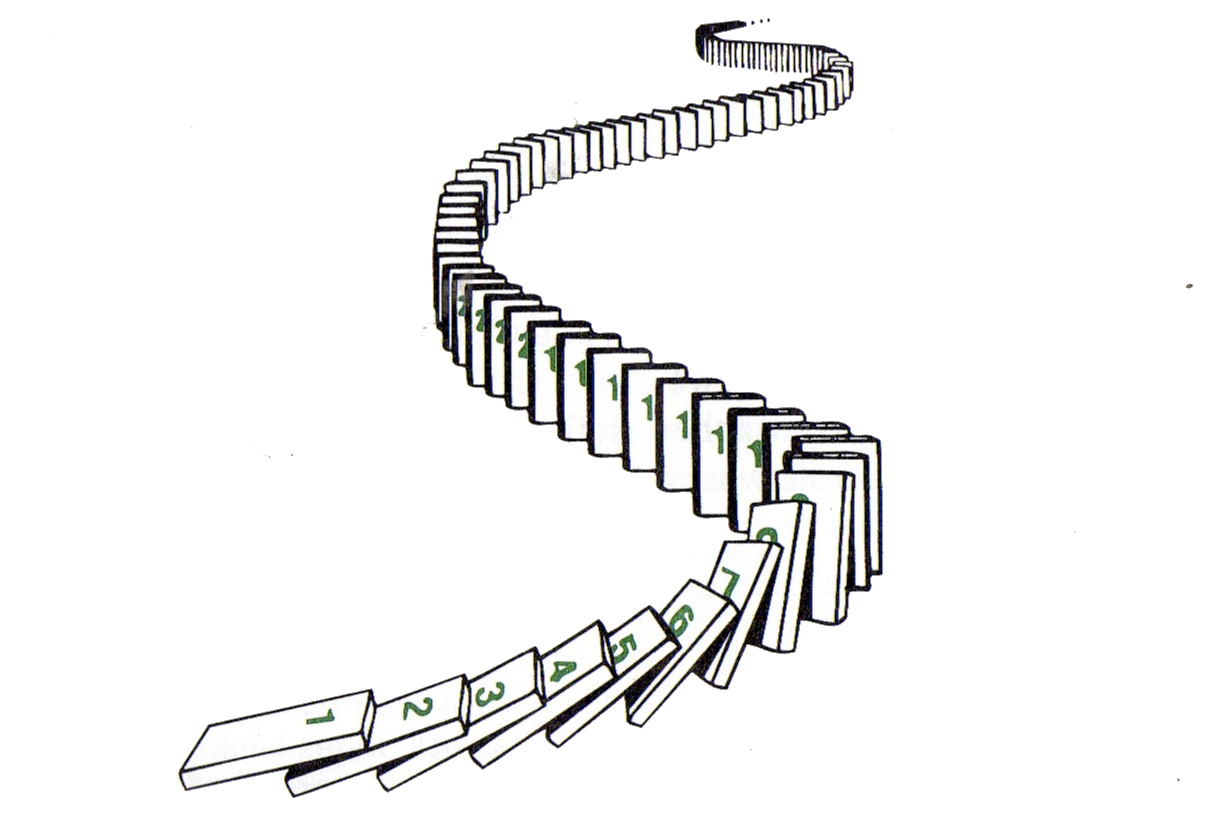
\includegraphics[width=0.4\textwidth]{Figures/domino.png}
    \caption{Ilustración del principio de inducción.}
\end{figure}
Esta técnica se puede visualizar como una fila de fichas de dominó: si la primera ficha cae y si al caer una ficha hace caer la siguiente, entonces todas las fichas caerán.


\begin{exampleblock}{Ejemplo: Suma de los primeros números naturales}
Probaremos por inducción que:
$$ 0 + 1 + \dots + n = \frac{n(n+1)}{2}. $$

\textbf{Caso base:} Para $n=0$, tenemos $0 = \frac{0(0+1)}{2}$, que es cierto.

\textbf{Caso inductivo:} Supongamos que la fórmula es válida para algún $n$, es decir,
$$ 0 + 1 + \dots + n = \frac{n(n+1)}{2}. $$

Queremos demostrar que también se cumple para $n+1$:
\begin{align*}
    0 + 1 + \dots + n + (n+1) &= \frac{n(n+1)}{2} + (n+1) \
    &= \frac{n(n+1) + 2(n+1)}{2} \
    &= \frac{(n+1)(n+2)}{2}.
\end{align*}

Por lo tanto, la propiedad se mantiene y queda demostrada por inducción.
\end{exampleblock}

\subsubsection*{Limitaciones del principio de inducción}
La inducción es una técnica muy útil para \alert{probar} versiones cerradas de fórmulas que involucran e.g. sumatorias, productorias o recurrencias, pero no nos dice
nada sobre cómo \alert{inferir} dichas formas cerradas. 

\subsection{Generalización del Principio de Inducción}

En algunas ocasiones, la propiedad que queremos demostrar no necesariamente comienza en $n=0$, sino en un valor inicial diferente, digamos $n_0$. En estos casos, podemos formular una versión más general del principio de inducción:

\begin{definitionblock}{Principio de Inducción Generalizado}
Si queremos demostrar que una propiedad $P(n)$ es válida para todos los números naturales mayores o iguales a un cierto $n_0$, basta con probar:
\begin{itemize}
    \item \textbf{Caso base:} Se demuestra que la propiedad es cierta para $n = n_0$.
    \item \textbf{Caso inductivo:} Se asume que la propiedad es cierta para un número arbitrario $n \geq n_0$ (hipótesis inductiva) y se demuestra que también es cierta para $n+1$.
\end{itemize}

Simbólicamente,
$$ P(n_0) \wedge \forall n \geq n_0 \; (P(n) \rightarrow P(n+1)) \Rightarrow \forall n \geq n_0. P(n). $$
\end{definitionblock}

Esta generalización es útil cuando la propiedad que queremos demostrar solo tiene sentido a partir de cierto número natural. Por ejemplo, si estamos probando una afirmación sobre la factorización de números naturales en factores primos, podríamos necesitar que el primer caso considerado sea $n_0 = 2$, ya que el número 1 no es primo ni compuesto.

\subsection*{Ejercicio: Lanzamiento de Pelotas en el Parque}
Un número impar de personas está de pie en un parque, cada una con una pelota en la mano. La distancia entre cualquier par de personas es distinta.

Cada persona lanza su pelota a la persona que está más cerca de ella. Queremos demostrar por inducción que \textbf{siempre existe al menos una persona que no recibe ninguna pelota}.

\medskip

Usando inducción, demostraremos la siguiente proposición \( P(n) \) sobre los números naturales mayores o iguales a 1:

\medskip

\begin{center}
  \( P(n) ~~\equiv~~ \)  Cuando en el parque se paran \( 2n+1 \) personas, existe una que no recibe ninguna pelota.
\end{center}
% \medskip

\subsubsection*{Caso base: \( P(1) \)}

Entre las tres personas, sean \( A \) y \( B \) las que están separadas por la menor distancia y \( C \) la persona restante, es decir:
\[
  d(A,B) < d(A,C) \quad \text{y} \quad d(A,B) < d(B,C).
\]

Como consecuencia, \( A \) y \( B \) se lanzan la pelota mutuamente, y por lo tanto, \( C \) no recibe ninguna pelota.

% \begin{figure}[h]
%     \centering
%     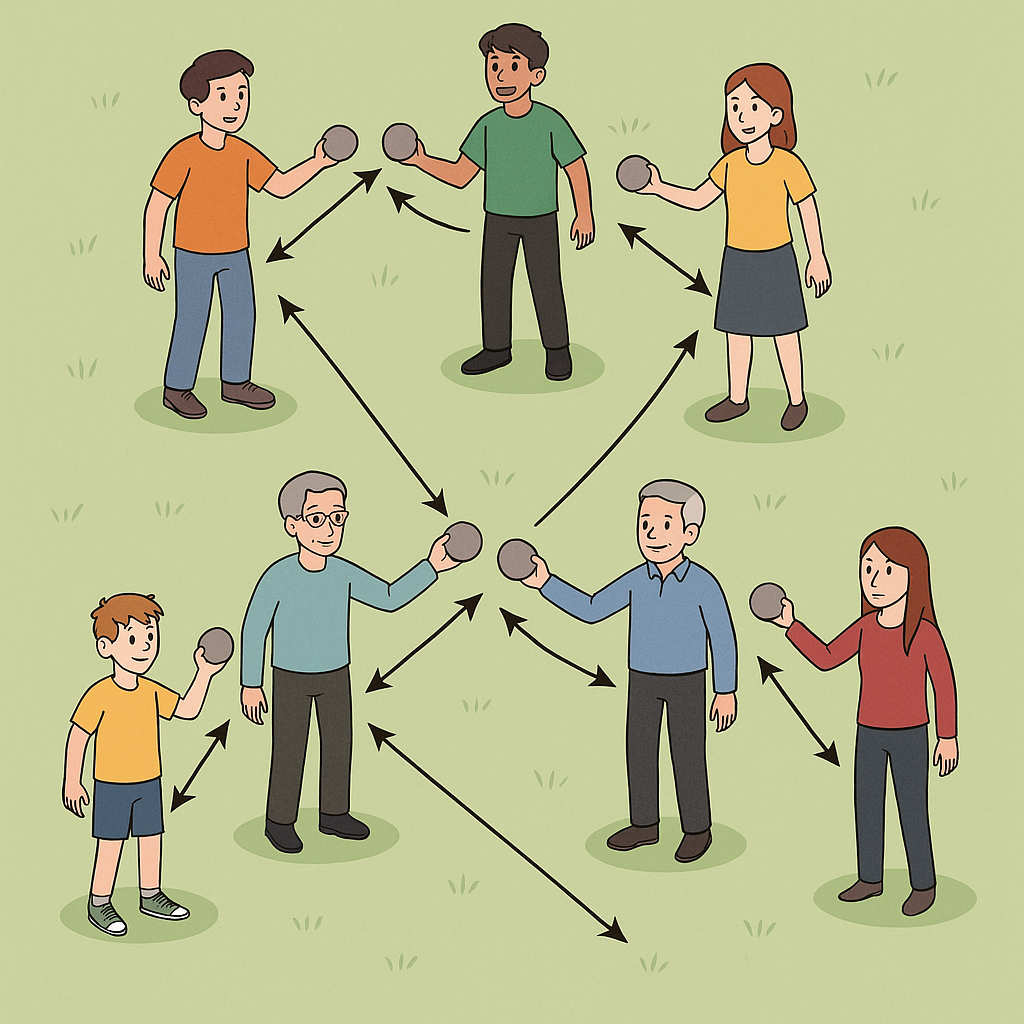
\includegraphics[width=0.2\textwidth]{Figures/ejercicio_induccion.png}
%     \caption{Ilustración del juego de pelotas en el parque.}
% \end{figure}

\subsubsection*{Caso inductivo}

Supongamos por hipótesis inductiva que en un grupo de \( 2n+1 \) personas siempre hay alguien que no recibe ninguna pelota. 
Queremos demostrar que lo mismo ocurre para \( 2n+3 \) personas.

Sean \( A \) y \( B \) las personas que están separadas por la menor distancia. Como en el caso base, \( A \) y \( B \) se lanzan la pelota mutuamente.

Ahora analizamos los siguientes casos:

\begin{itemize}
    \item Si alguien más le lanza su pelota a \( A \) o a \( B \), entonces el máximo de pelotas recibidas entre los restantes \( 2n+1 \) participantes es \( 2n \), y por tanto, al menos uno de ellos no recibe ninguna pelota.
    
    \item Supongamos que la única pelota que recibe \( A \) es la de \( B \), y viceversa. El resto del grupo es de \( 2n+1 \) personas, y todas las distancias entre ellas son distintas. Por hipótesis inductiva, alguien en este grupo no recibe ninguna pelota.
\end{itemize}

Por lo tanto, la proposición se mantiene para \( 2n+3 \), y el principio de inducción nos permite concluir que siempre habrá una persona que no recibe ninguna pelota en cualquier número impar de participantes.


\subsection{Ejercicios propuestos}

\begin{itemize}
    \item Demuestre que si $h > -1$, entonces para todo entero no negativo $n$ se tiene que $1+nh \leq (1+h)^n$.
    \item Demuestre que para todo entero positivo $n$ se tiene que $\sum_{i=1}^n \frac{1}{\sqrt{i}} > 2(\sqrt{n+1}-1)$.
    \item Sean $a_1,a_2,\dots,a_n$ números reales positivos. Probar que $$\frac{1}{n} (a_1+a_2+ \cdots + a_n) \geq (a_1 a_2 \cdots a_n)^{\frac{1}{n}}.$$ \end{itemize}


\section{Principio de Inducción Fuerte}
% \section{Simplificando el Caso Inductivo}

En el caso inductivo, para probar $P(n+1)$ sólo podemos emplear $$P(n)$$

Sin embargo, muchas pruebas se simplifican significativamente si pudiésemos emplear
$$P(0) \:\land\: P(1) \:\land\: \ldots \:\land\: P(n)$$

Este último argumento de prueba es válido y se conoce como \textbf{principio de inducción fuerte}.



\begin{definitionblock}{Principio de Inducción Fuerte}
Una propiedad vale para todos los números naturales si:

\begin{description}
\item[Caso base:] la propiedad vale para $0$.
\item[Caso inductivo:] cualquiera sea el natural $n$, la propiedad vale para $n+1$ si
  vale para todos los naturales menores o iguales a $n$.
\end{description}

Simbólicamente,
$$P(0) \,\wedge\, \forall n \;  ( P(0) \land P(1) \land \ldots \land P(n) ) \rightarrow P(n+1) \ \ \ 
\rightarrow \ \ \ \forall n.\ P(n)$$
\end{definitionblock}


\subsection{Ejercicio: Descomposición en Factores Primos}

Pruebe por inducción fuerte que todo natural mayor que 1 puede escribirse como producto (posiblemente unitario) de factores primos.

\textbf{Caso base:} Trivial ya que $2$ puede escribirse como el producto unitario $2$.

\textbf{Caso inductivo:} Considere el natural $n+1$ y asuma por hipótesis inductiva que todo natural en el intervalo $[2, n]$ puede escribirse como producto de factores primos. Ahora analicemos si $n+1$ es primo o compuesto.

\begin{itemize}
\item Si $n+1$ es primo, la propiedad es trivial.
\item Si $n+1$ es compuesto, entonces existen naturales $j,k$ en el intervalo $[2,n]$ tales que $n+1 = j \cdot k$. Por hipótesis inductiva, $j$ y $k$ pueden escribirse como producto de factores primos, y por lo tanto $n+1=j\cdot k$ también.
\end{itemize}

\textbf{Observación:} Para esta prueba usamos la variante del principio de inducción fuerte que establece la propiedad respectiva a partir de $2$ (no a partir de 0).



\subsection{Ejercicio: Cortando Barras de Chocolate}
\begin{wrapfigure}{r}{0.3\textwidth}
    \centering
    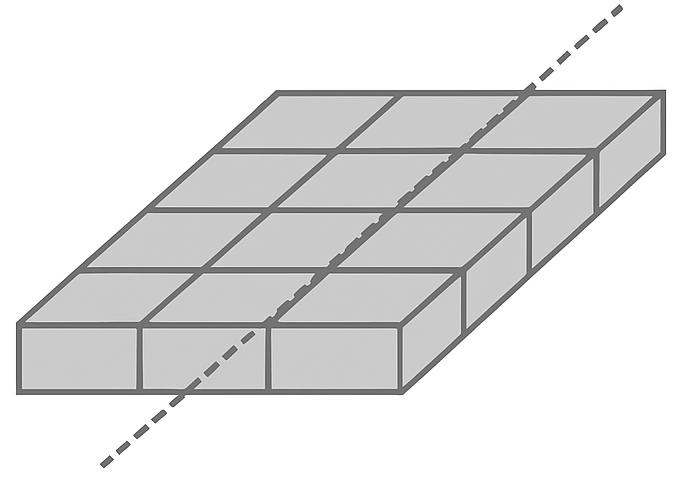
\includegraphics[width=0.22\textwidth]{Figures/barra.png}
    % \caption{Ilustración del principio de inducción.}
\end{wrapfigure}
Una barra de chocolate consiste en $m \times n$ cuadrados dispuestos en $m$ filas y $n$ columnas. Uno puede partir la barra en cuadrados  cortándola a lo largo de sus ``lineas''. Asumiendo que las lineas no se pueden cortar parcialmente, demuestre que $mn - 1$ cortes  alcanzan para obtener los  $mn$ cuadrados.

Haremos la demostración por inducción fuerte sobre el número $k=mn$ de cuadrados de la barra de chocolate.

\textbf{Caso base:} Una barra de $k=1$ cuadrado trivialmente puede ser cortada en cuadrados con $1-1$ cortes.

\textbf{Caso inductivo:} Consideremos una barra de $k+1$ cuadrados. Hagamos sobre la barra un corte arbitrario. Éste divide a la barra en dos subbarras de $k_1$ y $k_2$ cuadrados respectivamente, donde $k_1 + k_2 = k+1$.

Por hipótesis de inducción estas dos barras pueden ser cortadas con $$k_1 - 1 \quad \text{y} \quad k_2-1$$ cortes. Por tanto, la barra original (de $k+1$ cuadrados) puede cortarse con:
\begin{align*}
    1 \; + \; k_1 - 1  \; + \; k_2 - 1 &= k_1 + k_2 -1 \\
    &= k
\end{align*}

cortes. Así se demuestra que cualquier barra de chocolate de $mn$ cuadrados puede ser cortada en unidades utilizando exactamente $mn - 1$ cortes.

\section{Comparando los dos principios de inducción}

Los dos principios de inducción estudiados (el estándar---también llamado \emph{débil}---y el fuerte) son \textbf{igualmente expresivos}. Esto significa que una propiedad puede ser establecida usando uno si y sólo si puede ser establecida usando el otro. 

Ambos principios permiten demostrar afirmaciones sobre los números naturales, pero en algunos casos el uso del principio de inducción fuerte simplifica considerablemente la demostración, ya que en lugar de depender solo de \( P(n) \) para demostrar \( P(n+1) \), permite utilizar todas las propiedades anteriores \( P(0), P(1), ..., P(n) \).

\medskip
\medskip

\textbf{Ejercicio:} Derive el principio de inducción fuerte a partir del principio de inducción estándar. \textit{Hint:} Proceda por inducción.

% \textbf{Demostración: Derivación del Principio de Inducción Fuerte a partir del Principio de Inducción Estándar}

% Para demostrar que el principio de inducción fuerte se sigue del principio de inducción estándar, procedemos por inducción sobre \( n \):

% \begin{itemize}
%     \item \textbf{Caso base:} Para \( n=0 \), la hipótesis de inducción estándar nos garantiza que \( P(0) \) es cierto.
    
%     \item \textbf{Paso inductivo:} Supongamos que el principio de inducción estándar es válido y que se cumple que \( P(n) \rightarrow P(n+1) \). Queremos demostrar que el principio de inducción fuerte también es válido, es decir, que si \( P(0), P(1), ..., P(n) \) son verdaderos, entonces también lo es \( P(n+1) \).
    
%     Como el principio de inducción estándar garantiza que \( P(n) \) implica \( P(n+1) \), podemos ver que, si asumimos que todos los valores anteriores hasta \( P(n) \) son ciertos, entonces \( P(n+1) \) también debe serlo, ya que el último paso de la demostración depende exclusivamente de \( P(n) \), el cual hemos supuesto verdadero.
    
%     Por lo tanto, el principio de inducción fuerte es una consecuencia directa del principio de inducción estándar.
% \end{itemize}

\subsection{Principio del Buen Orden}

El principio del buen orden es un concepto fundamental en la teoría de números y es equivalente al principio de inducción. Nos dice que cualquier subconjunto no vacío de los números naturales tiene un elemento mínimo. Esto significa que no existen secuencias infinitamente decrecientes en los naturales.

\begin{definitionblock}{Principio del Buen Orden}
Sea \( S \) un subconjunto no vacío de los números naturales \( \mathbb{N} \). Entonces, existe un elemento mínimo \( m \in S \), es decir, un número \( m \) tal que para todo \( x \in S \), se cumple que \( m \leq x \).
\end{definitionblock}

El principio del buen orden es la base lógica de la inducción matemática, ya que podemos utilizarlo para demostrar el principio de inducción estándar por reducción al absurdo. La idea detrás de esta prueba es suponer que existe un número natural para el cual no se cumple la propiedad que queremos demostrar, y mostrar que esto lleva a una contradicción con el principio del buen orden.

\medskip
\medskip

\textbf{Ejercicio:} Derive el principio de inducción estándar a partir del principio del buen orden. \textit{Hint:} Proceda por reducción al absurdo.

% \textbf{Demostración: Derivación del Principio de Inducción Estándar a partir del Principio del Buen Orden}

% Supongamos que el principio de inducción estándar no es cierto. Es decir, existe un subconjunto de los números naturales \( S \) tal que:
% \begin{itemize}
%     \item Contiene todos los valores para los cuales la propiedad \( P(n) \) no es verdadera.
%     \item Este conjunto \( S \) es no vacío.
% \end{itemize}

% Por el principio del buen orden, sabemos que \( S \) tiene un elemento mínimo, digamos \( m \). Es decir, \( P(m) \) no es cierto, pero para todo número menor que \( m \), la propiedad sí se cumple.

% Ahora bien, por la hipótesis de inducción estándar, si \( P(k) \) es cierto para algún \( k \), entonces \( P(k+1) \) también lo es. Como todos los números menores que \( m \) cumplen \( P(n) \), se sigue que \( P(m) \) también debe cumplirse, lo cual es una contradicción.

% Por lo tanto, \( S \) debe ser vacío, lo que implica que el principio de inducción estándar es válido.


\medskip
\medskip

Es más, puede probarse que el principio de inducción débil, el principio de inducción fuerte y el principio del buen orden resultan \textbf{equivalentes}. En otras palabras, si se asume cualquiera de estos principios como cierto, se pueden demostrar los otros dos.


\section{Introducción a la Inducción Estructural}

La inducción es una técnica poderosa utilizada para demostrar propiedades de estructuras definidas recursivamente. Aunque la inducción matemática es útil para propiedades de los números naturales, la \textbf{inducción estructural} extiende esta idea a conjuntos definidos recursivamente.

A veces es difícil definir un objeto explícitamente, pero no lo es tanto si lo definimos en términos de objetos de su mismo tipo. A este proceso lo llamamos \textbf{recursión}. Mediante recursión, podemos definir secuencias, funciones y conjuntos, especificando un caso base y reglas que permiten construir nuevos elementos a partir de los ya existentes.


\subsection{Definiciones Recursivas}
\begin{definitionblock}{Definición Recursiva}
Un objeto puede definirse recursivamente especificando:
\begin{itemize}
    \item \textbf{Caso base}: Elementos iniciales del conjunto.
    \item \textbf{Regla recursiva}: Forma de construir nuevos elementos a partir de los ya definidos.
\end{itemize}
\end{definitionblock}
\subsubsection*{Ejemplo: Secuencia de Potencias de 2}
\begin{itemize}
    \item Caso base: $a_0 = 1$.
    \item Regla recursiva: $a_{n+1} = 2a_n$.
\end{itemize}
\noindent Aplicando esta definición recursiva, obtenemos los términos de la secuencia que generan las potencias de 2: $1, 2, 4, 8, 16, 32, \dots$.

La ventaja de definir una secuencia recursivamente es que no necesitamos conocer una fórmula explícita general desde el principio. En muchos casos, esto facilita la comprensión y el diseño de algoritmos que dependen de estructuras previas, como en el caso de la programación dinámica o la resolución de problemas combinatorios.


\subsection{Definición Recursiva de Funciones}
\subsubsection{Factorial}
Un ejemplo clásico de función definida recursivamente es el factorial. La función $f(n) = n!$ puede ser definida recursivamente como:
\[
    f(0) = 1, \quad f(n+1) = (n+1)f(n).
\]

\bigskip
\noindent \textbf{Ejercicio}: Defina recursivamente la función $S(n) = \sum_{k=0}^{n} a_k$.

\subsubsection{Números de Fibonacci}
Los números de Fibonacci están definidos por:
\begin{align*}
    f_0 &= 0, \quad f_1 = 1, \\
    f_n &= f_{n-1} + f_{n-2}, \quad \text{para } n \geq 2.
\end{align*}

Ejemplo: $0, 1, 1, 2, 3, 5, 8, 13, 21, \dots$

\subsubsection*{Ejercicio: Propiedad de Crecimiento de Fibonacci}
Demuestre que para todo $n \geq 3$, si $\alpha = \frac{1 + \sqrt{5}}{2}$, entonces $f_n > \alpha^{n-2}$.
\subsubsection*{Demostración por inducción:}
\noindent \textbf{Caso Base:} Debemos demostrar el caso base tanto para $n=3$ como para $n=4$ (porque no podemos demostrar que $f_4 > \alpha^2$ desde la hipótesis inductiva).

Esto no es difícil puesto que:
\begin{align*}
    f_3 &= 2 > \alpha = \frac{1 + \sqrt{5}}{2}, \\
    f_4 &= 3 > \alpha^2 = \frac{3 + \sqrt{5}}{2}.
\end{align*}

\noindent \textbf{Caso Inductivo:} Considere un entero $n + 1$ tal que $n \geq 4$. Por hipótesis inductiva, $f_j > \alpha^{j-2}$ para todo $j \in [3, n]$.

Dado que $f_{n+1} = f_n + f_{n-1}$, se tiene:
\[
    f_{n+1} > \alpha^{n-2} + \alpha^{n-3} = \alpha^{n-3} (1 + \alpha).
\]

Por tanto, para demostrar que $f_{n+1} > \alpha^{n-1}$ basta demostrar que:
\[
    (1 + \alpha) \geq \alpha^2.
\]

Esto es fácil, ya que:
\[
    (1 + \alpha) = \frac{3 + \sqrt{5}}{2} = \alpha^2.
\]

Así, la desigualdad se cumple y la demostración por inducción queda completada.

\bigskip
\noindent \textbf{Ejercicio}: Demuestre que para todo entero positivo $n$, 
 $$ f_0 f_1 + f_1 f_2 + \cdots + f_{2n-1} f_{2n} = f_{2n}^2. $$


\subsection{Conjuntos Definidos Recursivamente}
Los conjuntos también pueden definirse de manera recursiva, siguiendo una estructura similar a la de las funciones. Un conjunto recursivamente definido se construye especificando un conjunto base y una regla que permite generar nuevos elementos a partir de los que ya están en el conjunto.

La definición recursiva de conjuntos sigue la estructura:
\begin{itemize}
    \item \textbf{Caso base}: Elementos iniciales del conjunto.
    \item \textbf{Regla recursiva}: Forma de construir nuevos elementos.
\end{itemize}

\begin{exampleblock} {Definición de $\Sigma^*$} 
El conjunto de strings sobre un alfabeto $\Sigma$:
\begin{itemize}
    \item \textbf{Caso base}: La cadena vacía $\epsilon$ pertenece a $\Sigma^*$.
    \item \textbf{Regla recursiva}: Si $w \in \Sigma^*$ y $x \in \Sigma$, entonces $wx \in \Sigma^*$.
\end{itemize}
\end{exampleblock}
Este conjunto, denotado como $\Sigma^*$, representa todas las posibles cadenas (incluyendo la cadena vacía) que pueden formarse con los símbolos de $\Sigma$.

\subsubsection{Definiciones Recursivas de Operaciones sobre Strings}
Al igual que los conjuntos, las operaciones sobre strings pueden definirse de manera recursiva. Definir operaciones de esta manera nos permite formalizar algoritmos y probar propiedades sobre strings de manera estructurada.

Una de las operaciones más importantes sobre strings es la concatenación, que une dos strings en un solo. La concatenación de dos strings $w_1$ y $w_2$ se define recursivamente de la siguiente manera:
\begin{exampleblock}{Definición de concatenación}
\begin{itemize}
    \item \textbf{Regla base}: Si $w \in \Sigma^*$, entonces $w \cdot \epsilon = w$ (concatenar con la cadena vacía no cambia la cadena original).
    \item \textbf{Regla inductiva}: Si $w_1, w_2 \in \Sigma^*$ y $x \in \Sigma$, entonces $w_1 \cdot (w_2x) = (w_1 \cdot w_2) x$ (concatenar un carácter a una cadena es equivalente a concatenar primero el prefijo y luego agregar el carácter final).
\end{itemize}
\end{exampleblock}

Por ejemplo, si tenemos el alfabeto $\Sigma = \{a, b\}$ y las cadenas $w_1 = ab$, $w_2 = ba$, la concatenación $w_1 \cdot w_2$ sigue:
\begin{align*}
    ab \cdot ba &= (ab \cdot b)a \\
    &= ((ab \cdot \epsilon)b)a \\
    &= (ab)b)a \\
    &= abb a.
\end{align*}

Otra propiedad importante de los strings es su longitud. Podemos definir recursivamente la función $l(w)$, que calcula la longitud de un string $w$:
\begin{exampleblock}{Definición de longitud}
\begin{itemize}
    \item \textbf{Regla base}: $l(\epsilon) = 0$.
    \item \textbf{Regla inductiva}: $l(w x) = l(w) + 1$, para $x \in \Sigma$ (cada vez que agregamos un carácter a la cadena, su longitud aumenta en uno).
\end{itemize}
\end{exampleblock}

Por ejemplo, si $w = ab$:
\begin{align*}
    l(\epsilon) &= 0, \\
    l(a) &= l(\epsilon) + 1 = 1, \\
    l(ab) &= l(a) + 1 = 2.
\end{align*}

\section{Inducción Estructural sobre Estructuras Recursivas}
La \textbf{inducción estructural} es un método para demostrar propiedades de conjuntos definidos de manera recursiva. Dado que estos conjuntos están construidos a partir de reglas que generan nuevos elementos a partir de los anteriores, la inducción estructural nos permite razonar sobre ellos en una forma natural y efectiva.
La inducción estructural permite demostrar que una propiedad se cumple para todos los elementos del conjunto sin necesidad de verificarlos uno por uno.

El método de inducción estructural sigue estos pasos:
\begin{definitionblock}{Inducción Estructural}
\begin{itemize}
    \item \textbf{Caso base}:  Demostrar que la propiedad se cumple para cada caso base de
la definición recursiva.
    \item \textbf{Paso inductivo}: Se asume que la propiedad es cierta para los elementos ya definidos (hipótesis inductiva) y se prueba que debe ser cierta para los nuevos elementos generados por la regla recursiva.
\end{itemize}
\end{definitionblock}

\subsection{Ejemplo: Longitud de Cadenas}

\textbf{Ejercicio:} Demuestre que para todo par de strings $w_1, w_2 \in \Sigma^*$, se cumple:
\[
    l(w_1 w_2) = l(w_1) + l(w_2).
\]

\subsubsection*{Demostración}
\noindent Definimos la proposición $P(y)$ como:
\[
    l(x y) = l(x) + l(y) \quad \text{para cualquier } x \in \Sigma^*.
\]
Queremos probar que $P(y)$ es cierta para todo $y \in \Sigma^*$ usando inducción estructural.

\noindent \textbf{Caso base:} Si $y = \epsilon$ (cadena vacía), entonces:
\[
    l(x \epsilon) = l(x) = l(x) + 0 = l(x) + l(\epsilon).
\]
Esto muestra que la propiedad se cumple para el caso base.

\noindent \textbf{Paso inductivo:} Supongamos que la propiedad es cierta para una cadena $w$, es decir, que:
\[
    l(x w) = l(x) + l(w).
\]
Ahora, consideremos una cadena extendida con un símbolo adicional $a \in \Sigma$, es decir, $w a$. Queremos demostrar que:
\[
    l(x w a) = l(x) + l(w a).
\]
Por la definición recursiva de la longitud de un string, sabemos que:
\[
    l(w a) = l(w) + 1.
\]
Aplicando la hipótesis inductiva:
\begin{align*}
    l(x w a) &= l(x w) + 1 \\
    &= (l(x) + l(w)) + 1 \\
    &= l(x) + (l(w) + 1) \\
    &= l(x) + l(w a).
\end{align*}
Dado que hemos demostrado que la propiedad se mantiene en el caso base y en el paso inductivo, por el principio de inducción estructural, concluimos que la propiedad es cierta para toda cadena $y \in \Sigma^*$.

\subsection{Definición Recursiva de Árboles Binarios}
\begin{exampleblock}{Árbol Binario}
Un árbol binario completo se define como:
\begin{itemize}
    \item \textbf{Caso base:} Un árbol con un único nodo raíz $r$.
    \item \textbf{Regla recursiva:} Si $T_1$ y $T_2$ son árboles binarios completos, entonces $T = T_1 \cdot T_2$ es un árbol binario completo que consiste de una raíz r junto con arcos que unen a $r$ con la raíz del sub-árbol izquierdo $T_1$ y con la raíz del sub-árbol derecho $T_2$.
\end{itemize}
\end{exampleblock}

\subsubsection{Ejercicio: Número de Vértices en un Árbol Binario}
Defina recursivamente la función $n(T)$ que entrega el número de vértices de un árbol binario $T$.

\textbf{Solución:}
\begin{itemize}
    \item \textbf{Caso base}: Si $T$ está formado sólo por una raíz $r$, entonces $n(T) = 1$.
    \item \textbf{Regla inductiva}: Si $T_1$ y $T_2$ son árboles binarios completos, entonces el árbol binario completo $T = T_1 \cdot T_2$ tiene:
    \[
        n(T) = 1 + n(T_1) + n(T_2).
    \]
\end{itemize}

\subsubsection{Ejercicio: Altura de un Árbol Binario}
Defina la función $h(T)$ que entrega la distancia máxima entre la raíz de un árbol binario $T$ y una de sus hojas.

\textbf{Solución:}
\begin{itemize}
    \item \textbf{Caso base}: Si $T$ está formado sólo por una raíz $r$, entonces $h(T) = 0$.
    \item \textbf{Regla inductiva}: Si $T_1$ y $T_2$ son árboles binarios completos, entonces el árbol binario completo $T = T_1 \cdot T_2$ tiene:
    \[
        h(T) = 1 + \max(h(T_1), h(T_2)).
    \]
\end{itemize}

\subsubsection{Ejercicio: Relación entre $n(T)$ y $h(T)$}
Demuestre que para todo árbol binario completo $T$, se cumple que:
\[
    n(T) \leq 2^{h(T)+1} - 1.
\]

\textbf{Demostración por Inducción Estructural:}

\textbf{Caso base:} Si $T$ está formado sólo por una raíz $r$, entonces $n(T) = 1$ y $h(T) = 0$, por lo que:
\[
    n(T) = 1 \leq 2^{0+1} - 1 = 1.
\]

\textbf{Paso inductivo:} Supongamos que la propiedad se cumple para los subárboles $T_1$ y $T_2$, es decir,
\[
    n(T_1) \leq 2^{h(T_1)+1} - 1, \quad n(T_2) \leq 2^{h(T_2)+1} - 1.
\]

% Por las fórmulas recursivas de $n(T)$ y $h(T)$, tenemos:
% \[
%     n(T) = 1 + n(T_1) + n(T_2),
% \]
% \[
%     h(T) = 1 + \max(h(T_1), h(T_2)).
% \]

Utilizando la hipótesis inductiva:
\begin{align*}
n(T) &= 1 + n(T_1) + n(T_2) \quad  \\
&\leq 1 + (2^{h(T_1)+1 }- 1) + (2^{h(T_2)+1} - 1) \quad \text{por H.I.} \\
&\leq 2 \cdot \max(2^{h(T_1)+1} , 2^{h(T_2)+1}) - 1 \quad \text{suma es como máx 2 veces el mayor} \\
&= 2 \cdot 2^{max(h(T_1),h(T_2))+1} - 1 \quad \text{ } max(2^x,2^y) = 2^{max(x,y)} \\
&= 2 \cdot 2^{h(T)+1} - 1 \quad \text{por def. de } h(T) \\
&= 2^{h(T)+1} - 1.
\end{align*}


Por lo tanto, la propiedad se cumple para todo árbol binario completo $T$, completando la demostración.


% \section{Conclusión}
% La inducción estructural es una técnica esencial en matemáticas discretas y ciencias de la computación. Permite demostrar propiedades de estructuras definidas recursivamente, como funciones, secuencias, conjuntos y árboles binarios.


\subsection{Ejercicios Propuestos:}
\begin{itemize}
    % \item Demostrar que la concatenación de dos cadenas en $\Sigma^*$ es asociativa, es decir, para todo $x, y, z \in \Sigma^*$:
    % \[
    %     (x \cdot y) \cdot z = x \cdot (y \cdot z).
    % \]
     \item Definir recursivamente la función $rev(w)$ que invierte un string en $\Sigma^*$, y demostrar por inducción estructural que $rev(xy) = rev(y)rev(x)$ para todo $x, y \in \Sigma^*$.
    \item Sea $A$ el conjunto definido recursivamente por: \textbf{(i)} $\epsilon \in A$; \textbf{(ii)} si $w \in A$ entonces $awa \in A$, para $a \in \Sigma$. Demostrar que toda cadena en $A$ tiene longitud par.

    \item Definir recursivamente la función que cuenta el número de hojas en un árbol binario completo.
    \item Probar por inducción estructural que el número de hojas en un árbol binario completo de altura $h$ es exactamente $2^h$.
    \item Demostrar que en un árbol binario completo con $n$ nodos internos, hay exactamente $n+1$ hojas.
    \item Probar que la altura de un árbol binario completo con $n$ nodos es al menos $\log_2(n+1) - 1$.
\end{itemize}


\section{Ejercicios Resueltos}

\subsection{Ejercicio: Propiedad de la reversa de strings}

Definir recursivamente la función $rev(w)$ que invierte un string $w \in \Sigma^*$. Luego, demostrar por inducción estructural que:
\[
    \text{rev}(xy) = \text{rev}(y)\text{rev}(x)
\]
para todo $x, y \in \Sigma^*$.

\textbf{Definición recursiva de $\text{rev}(w)$:}
\begin{itemize}
    \item Caso base: $\text{rev}(\epsilon) = \epsilon$
    \item Paso recursivo: Si $w \in \Sigma^*$ y $a \in \Sigma$, entonces $\text{rev}(wa) = a \cdot \text{rev}(w)$
\end{itemize}

\textbf{Demostración:} Fijamos un string $x \in \Sigma^*$. Demostraremos por inducción estructural sobre $y$ que:
\[
    \text{rev}(xy) = \text{rev}(y) \cdot \text{rev}(x)
\]

\textbf{Caso base:} $y = \epsilon$
\[
    \text{rev}(x\epsilon) = \text{rev}(x) = \epsilon \cdot \text{rev}(x) = \text{rev}(\epsilon) \cdot \text{rev}(x)
\]

\textbf{Paso inductivo:} Supongamos que $\text{rev}(xw) = \text{rev}(w)\text{rev}(x)$ para una cadena $w \in \Sigma^*$. Queremos demostrar que también se cumple para $wa$, donde $a \in \Sigma$.
\begin{align*}
\text{rev}(xwa) &= a \cdot \text{rev}(xw) \\
                &= a \cdot (\text{rev}(w)\text{rev}(x)) \\
                &= (a \cdot \text{rev}(w)) \cdot \text{rev}(x) \\
                &= \text{rev}(wa) \cdot \text{rev}(x)
\end{align*}
Por lo tanto, se cumple la propiedad para todo $y \in \Sigma^*$.

\subsection{Ejercicio: Longitud par en un conjunto definido recursivamente}

Sea el conjunto $A$ definido por:
\begin{itemize}
    \item Caso base: $\epsilon \in A$
    \item Paso recursivo: Si $w \in A$ y $a \in \Sigma$, entonces $awa \in A$
\end{itemize}

Demostrar que toda cadena en $A$ tiene longitud par.

\textbf{Demostración por inducción estructural:}

\textbf{Caso base:} $\epsilon \in A$, y su longitud es $0$, que es par.

\textbf{Paso inductivo:} Supongamos que $|w|$ es par. Entonces $|awa| = |w| + 2$. Como $|w|$ es par, $|w| = 2k$ para algún $k$, por lo tanto:
\[
    |awa| = 2k + 2 = 2(k + 1)
\]
que es par.

Por lo tanto, toda cadena en $A$ tiene longitud par.

\newpage
\part{Relaciones y Funciones}
\chapter{Relaciones}
\section{Definición de relaciones}

\subsection{¿Qué es una relación?}


En matemáticas, una de las formas más naturales de establecer conexiones entre elementos de distintos conjuntos es a través de las relaciones.

En ciencias de la computación, las relaciones juegan un rol fundamental en múltiples contextos. Permiten modelar datos y sus vínculos, como en bases de datos relacionales; representan estructuras como grafos en algoritmos y redes; y son esenciales para describir transiciones de estado, dependencias, ordenamientos y equivalencias. Comprender las propiedades de las relaciones permite, por ejemplo, optimizar consultas en SQL, verificar invariantes en programas o formalizar sistemas lógicos complejos.


\begin{definitionblock}{Relación binaria}
Una \textbf{relación binaria} entre dos conjuntos $A$ y $B$ es un \textbf{subconjunto del producto cartesiano} $A \times B$. Es decir, es un conjunto de pares ordenados $(a,b)$ donde $a \in A$ y $b \in B$.
\end{definitionblock}

\paragraph{Notación.} Si $R \subseteq A \times B$, entonces decimos que los elementos $a_0 \in A$ y $b_0 \in B$ están relacionados por $R$ si $(a_0, b_0) \in R$. Esto lo denotamos como:
\[ a_0 \, R \, b_0. \]
Si no están relacionados, usamos:
\[ a_0 \, \centernot R \, b_0 \quad \text{ o } \quad (a_0, b_0) \notin R. \]

\subsubsection*{Ejemplo: Relación de divisibilidad.} Consideremos los conjuntos $\mathbb{N}$ (naturales) y $\mathbb{N}_0$ (naturales con cero). Podemos definir la relación de divisibilidad como:
\[
\mid \,=\, \{ (a, k \cdot a) \mid a \in \mathbb{N},~k \in \mathbb{N}_0 \}.
\]
Otra forma equivalente de definirla:
\[
a \mid b \quad \Leftrightarrow \quad \exists k \in \mathbb{N}_0 \text{ tal que } b = k \cdot a.
\]

\subsubsection*{Ejemplo: Base de datos relacional.} 
En una base de datos relacional, una relación puede modelar la asignación de estudiantes a cursos como un subconjunto del producto cartesiano entre el conjunto de estudiantes $E$ y el conjunto de cursos $C$. Por ejemplo, si $(e, c) \in R$ indica que el estudiante $e$ está inscrito en el curso $c$.
% $R \subseteq E \times C$ es una relación que puede analizarse para detectar redundancias, restricciones de integridad o prerequisitos utilizando propiedades como la transitividad o la unicidad.


\subsection{Representación de relaciones}
Cuando los conjuntos involucrados son finitos, podemos representar gráficamente una relación como un grafo dirigido. Una flecha desde $a \in A$ hacia $b \in B$ indica que $a \, R \, b$.


\begin{figure}[h]
\centering
\begin{tikzpicture}[every node/.style={circle,draw}, node distance=2cm]
  \node (a1) at (0,2) {$a_1$};
  \node (a2) at (0,0) {$a_2$};
  \node (b1) at (4,2.5) {$b_1$};
  \node (b2) at (4,0.5) {$b_2$};
  \node (b3) at (4,-1.5) {$b_3$};

  \draw[->] (a1) -- (b1);
  \draw[->] (a1) -- (b2);
  \draw[->] (a2) -- (b2);
  \draw[->] (a2) -- (b3);
\end{tikzpicture}
\caption{En esta ilustración, los nodos del lado izquierdo representan elementos de un conjunto $A$, los del lado derecho a un conjunto $B$, y las flechas indican los pares relacionados en $R \subseteq A \times B$.}
\end{figure}



\subsubsection*{¿Cuántas relaciones existen entre dos conjuntos finitos $A$ y $B$? }
Si $A$ tiene $m$ elementos y $B$ tiene $n$, entonces el conjunto $A \times B$ tiene $m \cdot n$ elementos. Por lo tanto, existen $2^{mn}$ relaciones distintas entre $A$ y $B$.

Esto muestro cómo una definición tan simple como ``subconjunto del producto cartesiano'' puede esconder una riqueza combinatoria enorme. Incluso con conjuntos pequeños, la cantidad de posibles relaciones crece exponencialmente. Esto tiene consecuencias profundas en ciencias de la computación. Por ejemplo,  en \textbf{bases de datos}, cada relación representa una tabla posible; entender su espacio total ayuda a evaluar restricciones, integridad referencial y optimización.
  



\subsection{Relaciones sobre un conjunto}

En el caso particular en que una relación $R$ relaciona elementos de un conjunto consigo mismo, es decir, $R \subseteq A \times A$, decimos que $R$ es una \textbf{relación sobre el conjunto $A$}.

\paragraph{Ejemplos.}
\begin{itemize}
  \item $R = \{(a,b) \mid a \leq b\}$ sobre $\mathbb{N}$.
  \item $R = \{(a,b) \mid a + b \leq 3\}$ también sobre $\mathbb{N}$.
\end{itemize}

\subsection{Propiedades de las relaciones}

Al estudiar relaciones sobre un conjunto $A$, es común interesarse por ciertas propiedades estructurales que éstas pueden tener. 
De hecho, cada una de estas propiedades ya las expresamos usando lógica de predicados. 


\begin{definitionblock}{Propiedades fundamentales}
Sea $R \subseteq A \times A$ una relación sobre $A$. Decimos que:
\begin{itemize}
  \item $R$ es \textbf{reflexiva} si $(a,a) \in R$ para todo $a \in A$.
  \item $R$ es \textbf{simétrica} si $(a,b) \in R$ implica $(b,a) \in R$.
  \item $R$ es \textbf{antisimétrica} si $(a,b) \in R$ y $(b,a) \in R$ implica $a = b$.
  \item $R$ es \textbf{transitiva} si $(a,b) \in R$ y $(b,c) \in R$ implica $(a,c) \in R$.
\end{itemize}
\end{definitionblock}



% \paragraph{Ejercicio.} ¿Qué propiedades cumple la relación vacía $R = \emptyset$?

\paragraph{Ejemplo:} Sobre el conjunto de enteros $\mathbb{Z}$:
\begin{itemize}
  \item $R_1 = \{(a,b) \mid a \leq b\}$ es reflexiva, antisimétrica y transitiva.
  \item $R_2 = \{(a,b) \mid a \mid b\}$ también cumple las tres propiedades anteriores.
  \item $R_3 = \{(a,b) \mid a + b \leq 3\}$ es simétrica, pero no transitiva ni reflexiva.
\end{itemize}

\section{Relaciones de orden}
Las relaciones de orden nos permiten capturar de manera formal la noción de jerarquía, precedencia o comparación entre elementos. Son fundamentales para modelar estructuras como cronogramas de tareas, jerarquías de clases, árboles de decisión, relaciones de dependencia en grafos y muchas otras situaciones donde ciertos elementos están "por encima" o "antes" que otros. 


\begin{definitionblock}{Relaciones de orden}
Una relación $R \subseteq A \times A$ se llama:
\begin{itemize}
  \item \textbf{Orden parcial} si es reflexiva, antisimétrica y transitiva.
  \item \textbf{Orden total} si además, para todo $a,b \in A$, se cumple que $(a,b) \in R$ o $(b,a) \in R$.
\end{itemize}
\end{definitionblock}

\paragraph{Ejemplo.}
\begin{itemize}
  \item La relación $\leq$ sobre $\mathbb{N}$ es un orden total.
  \item La inclusión $\subseteq$ sobre $2^S$ es un orden parcial, pero no total si $S \neq \emptyset$.
\end{itemize}



\section{Relaciones de equivalencia}
Las relaciones de equivalencia permiten formalizar la idea de que dos elementos son esencialmente ``lo mismo'' bajo cierto criterio. Estas relaciones son centrales para definir particiones de conjuntos, clases de objetos indistinguibles y estructuras algebraicas como clases de congruencia, espacios cociente o tipos abstractos de datos.

En ciencias de la computación, se usan para identificar elementos equivalentes en optimización de código, hashing, agrupamiento de datos y en la definición de semánticas de programas (por ejemplo, dos expresiones que se evalúan igual en todo contexto son consideradas equivalentes).


\begin{definitionblock}{Relación de equivalencia}
Una relación $R$ sobre un conjunto $A$ es una \textbf{relación de equivalencia} si es reflexiva, simétrica y transitiva.
\end{definitionblock}

\paragraph{Ejemplo: congruencia módulo $p$.} Para $p \geq 2$ y $a,b \in \mathbb{Z}$,
\[
a \equiv_p b \quad \Leftrightarrow \quad p \mid (a - b)
\]
es una relación de equivalencia.

% \paragraph{Ejercicio.} Demuestre que si $R$ es simétrica y transitiva, y para cada $a \in A$ existe $b$ tal que $(a,b) \in R$, entonces $R$ es reflexiva y por ende, una relación de equivalencia.




\bigskip
\begin{table}[h]
\centering
\resizebox{\textwidth}{!}{%
\begin{tabular}{|l|c|c|c|c|l|}
\hline
\textbf{Tipo de relación} & \textbf{Reflexiva} & \textbf{Simétrica} & \textbf{Antisimétrica} & \textbf{Transitiva} & \textbf{Ejemplo} \\
\hline
Relación de equivalencia & \checkmark & \checkmark & -- & \checkmark & Congruencia módulo $n$ \\
Orden parcial & \checkmark & -- & \checkmark & \checkmark & $\subseteq$, $\leq$ en $\mathbb{N}$ \\
Orden total & \checkmark & -- & \checkmark & \checkmark & $\leq$ en $\mathbb{Z}$ \\
\hline
\end{tabular}
}
\caption{Relación entre propiedades y tipos de relaciones comunes}
\end{table}

\subsection{Clases de equivalencia}
Una de las consecuencias más interesantes de tener una relación de equivalencia es que nos permite agrupar los elementos del conjunto en subconjuntos disjuntos llamados \textbf{clases de equivalencia}. Cada clase está formada por todos los elementos que son equivalentes entre sí respecto a la relación $R$. Esta idea permite clasificar elementos según algún criterio de equivalencia y es muy útil tanto en matemáticas como en ciencias de la computación, por ejemplo, al agrupar datos, detectar redundancias o definir estados equivalentes en autómatas.


\begin{definitionblock}{Clase de equivalencia}
Dada una relación de equivalencia $R$ sobre un conjunto $A$ y un elemento $a \in A$, la \textbf{clase de equivalencia} de $a$, denotada $[a]_R$, es:
\[
[a]_R = \{ b \in A \mid (a,b) \in R \}
\]
\end{definitionblock}

\paragraph{Ejemplo: módulo 3.}
\begin{align*}
[0]_{\equiv_3} &= \{ ..., -6, -3, 0, 3, 6, ... \} \\
[1]_{\equiv_3} &= \{ ..., -5, -2, 1, 4, 7, ... \} \\
[2]_{\equiv_3} &= \{ ..., -4, -1, 2, 5, 8, ... \}
\end{align*}

\begin{thmblock}{Lema: Caracterizaciones de equivalencia}  Si $R$ es una relación de equivalencia sobre $A$, entonces para cualquier $a, b \in A$ se cumple:
\[
(a,b) \in R \quad \Leftrightarrow \quad [a]_R = [b]_R \quad \Leftrightarrow \quad [a]_R \cap [b]_R \neq \emptyset
\]
\end{thmblock}
\begin{proof}
Demostremos las implicaciones una por una:

\begin{itemize}
  \item[$(1 \Rightarrow 2)$] Supongamos que $(a,b) \in R$. Queremos probar que $[a]_R = [b]_R$.\
  Sea $x \in [a]_R$, es decir, $(a,x) \in R$. Como $(a,b) \in R$ y $R$ es simétrica y transitiva, se sigue que $(b,x) \in R$, por lo tanto $x \in [b]_R$, y así $[a]_R \subseteq [b]_R$.\
  Análogamente, $(b,a) \in R$ (por simetría), y el mismo argumento muestra que $[b]_R \subseteq [a]_R$. Entonces $[a]_R = [b]_R$.

  \item[$(2 \Rightarrow 3)$] Supongamos que $[a]_R = [b]_R$. Entonces tienen al menos un elemento en común (por ejemplo $a \in [a]_R$), por lo tanto $[a]_R \cap [b]_R \neq \emptyset$.

  \item[$(3 \Rightarrow 1)$] Supongamos que $[a]_R \cap [b]_R \neq \emptyset$. Entonces existe $x \in A$ tal que $(a,x) \in R$ y $(b,x) \in R$. Como $R$ es simétrica, $(x,b) \in R$ y luego por transitividad, $(a,b) \in R$.
\end{itemize}
Por lo tanto, todas las implicaciones se cumplen y las tres condiciones son equivalentes.
\end{proof}


\section{Relaciones de equivalencia y particiones}

Vimos cómo una relación de equivalencia nos permite agrupar los elementos de un conjunto en clases de equivalencia, donde todos los elementos de una clase están relacionados entre sí. Esta estructura naturalmente nos lleva a la noción de \textbf{partición}, que es una forma de dividir un conjunto en subconjuntos que no se superponen y que cubren completamente al conjunto original.

Las clases de equivalencia inducidas por una relación de equivalencia forman una partición del conjunto. 
Inversamente, toda partición de un conjunto define una relación de equivalencia entre elementos. 
% Esta correspondencia entre relaciones de equivalencia y particiones es una idea fundamental que aparece en múltiples áreas de la matemática y la computación, desde estructuras algebraicas hasta clasificación de datos o estados equivalentes en autómatas.

\bigskip
\begin{definitionblock}{Partición}
Una \textbf{partición} de un conjunto $A$ es una colección de subconjuntos no vacíos, disjuntos dos a dos, cuya unión es $A$.
\end{definitionblock}

\begin{figure}[h]
\begin{center}
\begin{tikzpicture}[scale=1]
  \def\r{2}
  % Dibujamos el círculo completo
  \draw[thick] (0,0) circle (\r);

  % Llenamos los 3 sectores, cada uno cubriendo 120° del círculo
  \fill[blue!20] (0,0) -- (0:\r) arc (0:120:\r) -- cycle;
  \fill[green!20] (0,0) -- (120:\r) arc (120:240:\r) -- cycle;
  \fill[red!20] (0,0) -- (240:\r) arc (240:360:\r) -- cycle;

  % Etiquetamos cada sector
  \node at (60:1.4) {$A_1$};
  \node at (180:1.4) {$A_2$};
  \node at (300:1.4) {$A_3$};
  \node at (-2,1.8) {\bm{$A$}};
\end{tikzpicture}
\end{center}
\caption{En esta ilustración, el conjunto $A$ está dividido en tres subconjuntos disjuntos $A_1$, $A_2$ y $A_3$, que juntos forman una partición de $A$. Cada elemento del conjunto $A$ pertenece a uno y solo uno de los subconjuntos.}
\end{figure}



\paragraph{Ejemplo.}
\begin{itemize}
  \item $\{ \{2\}, \{1,3,4,5,\ldots\} \}$ es una partición de $\mathbb{N}$.
  \item $\{ \text{pares}, \text{impares} \}$ también lo es.
\end{itemize}

\begin{thmblock}{Teorema: Relaciones de equivalencia inducen particiones}
Si $R$ es una relación de equivalencia sobre $A$, entonces:
\[
\{ [a]_R \mid a \in A \}
\]
es una partición de $A$. Esta colección se llama \textbf{conjunto cociente}, denotado $A/\!_R$.
\end{thmblock}

\begin{proof}
Sea $R$ una relación de equivalencia sobre $A$. Debemos probar que el conjunto de clases de equivalencia $\{ [a]_R \mid a \in A \}$ cumple con las tres condiciones de una partición:
\begin{itemize}
  \item \textbf{No vacías:} Por reflexividad, todo $a \in A$ pertenece a su propia clase $[a]_R$, ya que $(a,a) \in R$. Por lo tanto, cada clase $[a]_R$ contiene al menos un elemento.
  \item \textbf{Disjuntas dos a dos:} $[a]_R \cap [b]_R \neq \emptyset \Leftrightarrow [a]_R = [b]_R $. Por lo tanto, dos clases de equivalencia o son idénticas o son disjuntas.
  \item \textbf{Cubren $A$:} Para todo $a \in A$, $a \in [a]_R$ por reflexividad. Entonces cada elemento pertenece a alguna clase.
\end{itemize}
Por lo tanto, $\{ [a]_R \mid a \in A \}$ es una partición de $A$.
\end{proof}

\paragraph{Ejemplo.} Dado la relación de congruencia módulo 3, la siguiente es una partición de $\mathbb{Z}$:
\[
\mathbb{Z}/\!_{\equiv_3} = \{ [0]_{\equiv_3}, [1]_{\equiv_3}, [2]_{\equiv_3} \}
\]

\begin{thmblock}{Teorema: Particiones inducen relaciones de equivalencia}
Dada una partición $\{A_i | i \in I\}$ de un conjunto $A$, existe una relación de equivalencia $R$ sobre $A$ cuyas clases de equivalencia son precisamente los conjuntos $A_i$.
\end{thmblock}
\begin{proof}
Definamos una relación $R$ sobre $A$ de la siguiente manera: para $x, y \in A$, decimos que $(x,y) \in R$ si y sólo si existen $i \in I$ tal que $x \in A_i$ y $y \in A_i$, es decir, si $x$ y $y$ pertenecen al mismo conjunto de la partición.

Vamos a demostrar que $R$ es una relación de equivalencia:
\begin{itemize}
  \item \textbf{Reflexiva:} Como $x \in A_i$ para algún $i$, se tiene que $(x,x) \in R$ porque $x$ y $x$ pertenecen al mismo conjunto.
  \item \textbf{Simétrica:} Si $(x,y) \in R$, entonces $x,y \in A_i$ para algún $i$, por lo tanto también $(y,x) \in R$.
  \item \textbf{Transitiva:} Si $(x,y) \in R$ y $(y,z) \in R$, entonces $x,y \in A_i$ y $y,z \in A_j$ para algunos $i,j \in I$. Pero como $y$ pertenece a ambos y los $A_i$ son disjuntos dos a dos, se deduce que $i = j$, y por lo tanto $x,z \in A_i$, así que $(x,z) \in R$.
\end{itemize}
Así, $R$ es una relación de equivalencia y sus clases de equivalencia son exactamente los conjuntos $A_i$.
\end{proof}

\subsection{Relaciones n-arias}
Hasta ahora nos hemos centrado en las relaciones binarias, es decir, aquellas que vinculan pares de elementos. Sin embargo, en muchas aplicaciones necesitamos expresar relaciones entre tres o más elementos. Esto nos lleva al concepto de \textbf{relaciones n-arias}, que generalizan la noción de relación binaria a tuplas de longitud arbitraria.

Estas relaciones aparecen frecuentemente en bases de datos relacionales (donde una tabla puede tener múltiples columnas) y  en especificaciones lógicas de sistemas (como restricciones que involucran varios objetos).


\begin{definitionblock}{Relación n-aria}
Una \textbf{relación $n$-aria} sobre un conjunto $A$ es un subconjunto de $A^n = A \times A \times \cdots \times A$ ($n$ veces).
\end{definitionblock}

\paragraph{Ejemplos.}
\begin{itemize}
  \item La propiedad de ser primo es una relación unaria sobre $\mathbb{N}$.
  \item La suma puede verse como una relación ternaria: $(a,b,c) \in \mathbb{N}^3$ tal que $a + b = c$.
  \item En una base de datos, una tabla con atributos (ID, nombre, curso) puede verse como una relación ternaria entre personas y cursos.
  \item En programación lógica, una relación cuaternaria puede expresar que un algoritmo transforma una entrada y un estado inicial en una salida y un nuevo estado.
\end{itemize}

\subsubsection*{¿Cuántas relaciones n-arias hay sobre un conjunto finito $A$?}
Primero observemos que una relación n-aria sobre $A$ es simplemente un subconjunto del conjunto de todas las $n$-uplas posibles de elementos de $A$, es decir, de $A^n$.
Si el conjunto $A$ tiene $k$ elementos (es decir, $|A| = k$), entonces, para cada elementos se puede decidir si está o no en la relación, el número total de relaciones n-arias posibles sobre $A$ es: $2^{k^n}$

\chapter{Funciones}

% \title{Apunte de Matemáticas Discretas CC3101:\\ Relaciones y funciones Clase 10}
% % \title{Ejercicios Lógica e Inducción}
% \author{Andrés Abeliuk}
% \date{}
% \maketitle


\section{Operaciones sobre Relaciones}

En esta secci\'on abordaremos c\'omo se pueden manipular las relaciones mediante operaciones, algunas heredadas de la teor\'ia de conjuntos y otras espec\'ificas de las relaciones. Esto permite construir relaciones m\'as complejas a partir de otras m\'as simples, analizar sus propiedades y establecer conexiones entre distintas estructuras.

\subsection{Operaciones Cl\'asicas: Uni\'on, Intersecci\'on y Diferencia}

Dado que una relaci\'on $R$ sobre un conjunto $A$ es un subconjunto de $A \times A$, podemos aplicar las operaciones usuales de conjuntos para combinarlas:

\begin{itemize}
  \item \textbf{Uni\'on:} $R \cup R'$ contiene todos los pares que pertenecen a $R$, a $R'$ o a ambos.
  \item \textbf{Intersecci\'on:} $R \cap R'$ contiene solo los pares comunes a ambas relaciones.
  \item \textbf{Diferencia:} $R \setminus R'$ contiene los pares que est\'an en $R$ pero no en $R'$.
\end{itemize}

Estas operaciones nos permiten combinar o contrastar relaciones distintas, como por ejemplo, intersectar relaciones de amistad y colaboraci\'on en redes sociales.


%
\subsection{Operaciones Espec\'ificas sobre Relaciones}

Adem\'as de las operaciones anteriores, existen operaciones espec\'ificas para relaciones:

\begin{itemize}
  \item \textbf{Inversi\'on:} La relaci\'on inversa de $R$ se denota $R^{-1}$ y consiste en invertir el orden de todos los pares: $R^{-1} = \{(b,a) \mid (a,b) \in R\}$.

  \item \textbf{Composici\'on:} Dadas dos relaciones $R \subseteq A \times B$ y $R' \subseteq B \times C$, su composici\'on es:
  \[ R' \circ R = \{(a,c) \mid \exists b. (a,b) \in R \land (b,c) \in R'\}. \]
  Esta operaci\'on se interpreta como ``relaci\'on indirecta'' a trav\'es de un intermediario.

  \item \textbf{Potencia:} Si $R$ es una relaci\'on sobre un conjunto $A$, definimos inductivamente:
  \[ R^1 = R, \quad R^{n+1} = R^n \circ R. \]
\end{itemize}

% Estas operaciones permiten, por ejemplo, analizar caminos de longitud $n$ en grafos (pensando en $R$ como relaci\'on de adyacencia).

\begin{figure}[H]
\centering
\begin{tikzpicture}[scale=1]

  % Conjuntos A, B, C
  \node (a1) at (0,2) {$a_1$};
  \node (a2) at (0,0) {$a_2$};

  \node (b1) at (3,2) {$b_1$};
  \node (b2) at (3,0) {$b_2$};

  \node (c1) at (6,2) {$c_1$};
  \node (c2) at (6,0) {$c_2$};

  % R: A -> B
  \draw[->, thick, blue] (a1) -- (b1);
  \draw[->, thick, blue] (a2) -- (b2);

  % S: B -> C
  \draw[->, thick, red] (b1) -- (c2);
  \draw[->, thick, red] (b2) -- (c1);

  % Composition: A -> C
  \draw[->, thick, dashed, violet] (a1) to[bend left=15] (c2);
  \draw[->, thick, dashed, violet] (a2) to[bend right=15] (c1);

  % Labels
  \node at (0,3.2) {$A$};
  \node at (3,3.2) {$B$};
  \node at (6,3.2) {$C$};

  % Legends
  \node[blue] at (1.5,2.6) {$R$};
  \node[red] at (4.5,2.6) {$S$};
  \node[violet] at (3, -1.2) {$S \circ R$};
\end{tikzpicture}
\caption{Composición de relaciones. Las flechas azules representan la relación \(R \subseteq A \times B\) y las rojas la relación \(S \subseteq B \times C\). La composición \(S \circ R \subseteq A \times C\) se indica con flechas punteadas moradas, que conectan elementos de \(A\) con \(C\) cuando existe un elemento intermedio en \(B\) que los vincula a través de \(R\) y \(S\).}
\end{figure}


\subsection*{Ejercicios resueltos}
\begin{exampleblock}{1. Transitividad y potencias:} Demostrar que $R$ es transitiva si y solo si $R^n \subseteq R$ para todo $n \geq 1$.

\emph{($\Rightarrow$)} Supongamos que $R$ es transitiva. Usamos inducción sobre $n$:

\textit{Caso base:} $n = 1$. Claramente $R^1 = R \subseteq R$.

\textit{Paso inductivo:} Supongamos que $R^k \subseteq R$. Entonces:
\[ R^{k+1} = R^k \circ R \subseteq R \circ R \subseteq R \]
por transitividad. Así, por inducción, $R^n \subseteq R$ para todo $n \geq 1$.

\emph{($\Leftarrow$)} Supongamos que $R^n \subseteq R$ para todo $n \geq 1$. En particular, $R^2 \subseteq R$ implica que $(a,b) \in R$ y $(b,c) \in R$ lleva a $(a,c) \in R^2 \subseteq R$, es decir, $R$ es transitiva.
\end{exampleblock}
\bigskip
\begin{exampleblock}{2. Simetría:} Demostrar que $R$ es simétrica si y solo si $R = R^{-1}$.

\emph{($\Rightarrow$)} Si $R$ es simétrica, entonces $(a,b) \in R$ implica $(b,a) \in R$, por lo tanto $R \subseteq R^{-1}$ y también $R^{-1} \subseteq R$, ya que si $(a,b) \in R^{-1}$ entonces $(b,a) \in R$ y por simetría $(a,b) \in R$. Así, $R = R^{-1}$.

\emph{($\Leftarrow$)} Si $R = R^{-1}$, entonces todo $(a,b) \in R$ satisface que $(b,a) \in R$, lo cual es precisamente la definición de simetría.
\end{exampleblock}
\bigskip
\begin{exampleblock}{3. Potencias de relación simétrica:} Sea $R$ simétrica. Demostrar que $R^n$ es simétrica para todo $n \geq 1$.

Demostramos por inducción sobre $n$ que $R^n$ es simétrica.

\textit{Caso base:} $n = 1$. $R^1 = R$ es simétrica por hipótesis.

\textit{Paso inductivo:} Supongamos que $R^k$ es simétrica. Consideremos $R^{k+1} = R^k \circ R$. Tomemos $(a,c) \in R^{k+1}$, entonces existe $b$ tal que $(a,b) \in R^k$ y $(b,c) \in R$. Por hipótesis, $(b,a) \in R^k$ y $(c,b) \in R$. Entonces $(c,a) \in R^{k+1}$, y se concluye que $R^{k+1}$ también es simétrica.

Así, $R^n$ es simétrica para todo $n \geq 1$.
\end{exampleblock}


\section{Clausuras}

Una clausura de una relaci\'on consiste en extenderla para que satisfaga una propiedad deseada (reflexividad, simetr\'ia o transitividad), agregando la menor cantidad posible de pares.

\begin{definitionblock}{Clausura}
Dada una relaci\'on $R$ sobre un conjunto $A$, su clausura reflexiva/sim\'etrica/transitiva es la \emph{menor} relaci\'on (en t\'erminos de inclusi\'on) que contiene a $R$ y que es reflexiva/sim\'etrica/transitiva, respectivamente.
\end{definitionblock}

\subsection{Clausura Reflexiva}

Se obtiene agregando todos los pares $(a,a)$ para cada $a \in A$ que no estaban ya en $R$.

\begin{exampleblock}{Ejemplo}
La clausura reflexiva de la relaci\'on $<$ sobre $\mathbb{N}$ es $\leq$.
\end{exampleblock}

\subsection{Clausura Sim\'etrica}

Para obtener la clausura sim\'etrica de una relaci\'on $R$, se agregan todos los pares $(b,a)$ tales que $(a,b) \in R$ pero $(b,a) \not\in R$.

\begin{exampleblock}{Ejemplo}
La clausura sim\'etrica de $R = \{(a,b) \mid a > b\}$ es $R \cup R^{-1} = \{(a,b) \mid a \neq b\}$.
\end{exampleblock}

\subsection{Clausura Transitiva}

La clausura transitiva de $R$ incluye todos los pares que se pueden alcanzar transitivamente:
\[ R^+ = \bigcup_{n=1}^{\infty} R^n. \]

La clausura reflexiva-transitiva se denota $R^* = R^+ \cup \{(a,a) \mid a \in A\}$.

\begin{exampleblock}{Ejemplo}
La clausura transitiva de la relaci\'on ``sucesor'' en $\mathbb{N}$ es la relaci\'on de orden $>$.
\end{exampleblock}


\begin{thmblock}{Lema}
Sea $R$ una relaci\'on sobre un conjunto finito $A$ con $|A| = n$. Demuestre que:
\[ R^+ = \bigcup_{1 \leq i \leq n} R^i. \]
\end{thmblock}
\begin{proof}
La clausura transitiva \( R^+ \) contiene todos los pares \((a,b)\) tales que existe un camino desde \( a \) hasta \( b \) siguiendo pasos de la relación \( R \).

En un conjunto finito con \( n \) elementos, cualquier secuencia de pasos que conecta dos elementos no necesita tener más de \( n \) pasos: si un camino tiene más de \( n \) nodos, entonces alguno se repite (por el principio del palomar que veremos en la próxima clase), y el camino puede acortarse eliminando ciclos.

Por lo tanto, para encontrar todos los pares conectados transitivamente, basta con considerar composiciones de \( R \) hasta longitud \( n \). 
\end{proof}

\begin{center}
\begin{tikzpicture}[->, thick, node distance=2cm]
  % Nodos
  \node[circle,draw] (a0) at (0,0) {$a_0$};
  \node[circle,draw] (a1) at (2,0) {$a_1$};
  \node[circle,draw] (a2) at (4,0) {$a_2$};
  \node[circle,draw] (a3) at (6,0) {$a_3$};

  % Camino
  \draw[->] (a0) -- (a1);
  \draw[->] (a1) -- (a2);
  \draw[->] (a2) -- (a3);

  \draw[->, bend left=40, red, dashed] (a3) to node[above, sloped] {\scriptsize ciclo} (a1);

  % Nota
  \node at (3,-1.3) {\footnotesize Se repite el nodo $a_1$: el camino contiene un ciclo};
\end{tikzpicture}
\end{center}

\vspace{-0.5em}
\begin{center}
\textit{Figura:} Un camino de más de \( n \) pasos en un conjunto de \( n \) elementos debe repetir nodos. 
% El ciclo puede eliminarse, acortando el camino sin perder la conexión entre extremos.
\end{center}




\begin{exampleblock}{Ejemplo: Clausura transitiva en planificación de tareas}

Supongamos que tenemos un conjunto de tareas \( A = \{\text{A}, \text{B}, \text{C}, \text{D}\} \) en un proyecto. La relación \( R \subseteq A \times A \) indica dependencias directas: si \( (x, y) \in R \), entonces la tarea \( x \) debe completarse antes de comenzar la tarea \( y \).

Sean las dependencias directas:
\[
R = \{ (\text{A}, \text{B}), (\text{B}, \text{C}), (\text{C}, \text{D}) \}
\]

\textbf{Objetivo:} Calcular la clausura transitiva \( R^+ \), que representa todas las tareas que deben realizarse antes de otra, directa o indirectamente.

\textbf{Cálculo de \( R^+ \):}
\[
\begin{aligned}
R^1 &= R = \{ (\text{A}, \text{B}), (\text{B}, \text{C}), (\text{C}, \text{D}) \} \\\\
R^2 &= \{ (\text{A}, \text{C}), (\text{B}, \text{D}) \} \\\\
R^3 &= \{ (\text{A}, \text{D}) \} \\\\
R^+ &= R \cup R^2 \cup R^3 = \{ (\text{A}, \text{B}), (\text{B}, \text{C}), (\text{C}, \text{D}), (\text{A}, \text{C}), (\text{B}, \text{D}), (\text{A}, \text{D}) \}
\end{aligned}
\]

\textbf{Representación gráfica:}

\begin{center}
\begin{tikzpicture}[->, node distance=2cm, thick]
  \node (A) at (0, 0) {A};
  \node (B) at (2, 1.5) {B};
  \node (C) at (4, 1.5) {C};
  \node (D) at (6, 0) {D};

  % relaciones directas (R)
  \draw[->, blue] (A) -- (B);
  \draw[->, blue] (B) -- (C);
  \draw[->, blue] (C) -- (D);

  % relaciones transitivas (R+ \ R)
  \draw[->, dashed, red] (A) to[bend left=15] (C);
  \draw[->, dashed, red] (B) to[bend left=15] (D);
  \draw[->, dashed, red] (A) to[bend left=30] (D);
\end{tikzpicture}
\end{center}

\vspace{1mm}
{\small
\textcolor{blue}{Azul}: dependencias directas. \quad
\textcolor{red}{Rojo punteado}: dependencias inferidas transitivamente.
}

\end{exampleblock}


\section{Funciones}

\begin{definitionblock}{Funci\'on}
Una funci\'on $f: A \to B$ es una relaci\'on que a cada elemento $a \in A$ le asigna \emph{un \'unico} elemento $b \in B$. Se denota $f(a) = b$.
\end{definitionblock}

\noindent Dado $a \in A$ escribimos \textbf{$f(a)$} para denotar al \emph{único} $b \in B$ tal que $(a,b) \in f$. En este caso decimos que $b$ es la \textbf{imagen} de $a$ (o que $a$ es una \textbf{preimagen} de $b$).


\noindent El conjunto $A$ se llama \emph{dominio} y el conjunto $\{b \in B \mid \exists a \in A, f(a) = b\}$ se llama \emph{rango}.

\subsection{Clasificaci\'on de funciones}

\begin{itemize}
  \item \textbf{Inyectiva (uno a uno):} Si $a_1 \neq a_2$ implica $f(a_1) \neq f(a_2)$.
  \item \textbf{Sobreyectiva (sobre):} Si todo $b \in B$ tiene una preimagen en $A$.
  \item \textbf{Biyectiva:} Si es inyectiva y sobreyectiva.
\end{itemize}

\begin{exampleblock}{Ejemplos}
La funci\'on $f:\mathbb{N}_0 \to \mathbb{N}_0$ dada por $f(n) = 2n$ es inyectiva pero no sobreyectiva.

La funci\'on $f:\mathbb{N}_0 \to \mathbb{N}_0$ dada por $f(0) = 1$, $f(n) = n-1$ para $n>0$, es sobreyectiva pero no inyectiva.
\end{exampleblock}

\subsection{Operaciones con funciones}

\begin{itemize}
  \item \textbf{Composici\'on:} Dados $f: A \to B$ y $g: B \to C$, se define $g \circ f: A \to C$ por $g(f(a))$.
  \item \textbf{Inversa:} Si $f$ es biyectiva, entonces existe $f^{-1}: B \to A$ tal que $f^{-1}(f(a)) = a$.
\end{itemize}

\begin{exampleblock}{Ejercicio Propuesto}
Demuestre que si $f$ y $g$ son inyectivas (resp. sobreyectivas), entonces $g \circ f$ tambi\'en lo es.
\end{exampleblock}

\section{Crecimiento de Funciones}

Para comparar el comportamiento asint\'otico de funciones, usamos la notaci\'on $O$:

\begin{definitionblock}{Notaci\'on $O$}
Dadas funciones $f$ y $g$, decimos que $f(x)$ es $O(g(x))$ si existen constantes $c, k > 0$ tales que:
\[ f(x) \leq c \cdot g(x), \quad \forall x > k. \]
\end{definitionblock}

\begin{exampleblock}{Ejercicios Propuestos}
\begin{itemize}
\item Demuestre que $f(x) = x^2 + 2x + 1$ es $O(x^2)$.
\item Demuestre que todo polinomio de grado $n$ con coeficientes reales es $O(x^n)$.
\end{itemize}
\end{exampleblock}

\subsection{Composici\'on de funciones en t\'erminos de $O$}

\begin{thmblock}{Teorema}
Si $f_1 = O(g_1(x))$ y $f_2 = O(g_2(x))$, entonces:
\begin{itemize}
  \item $f_1(x) + f_2(x) = O(\max\{g_1(x), g_2(x)\})$.
  \item $f_1(x) \cdot f_2(x) = O(g_1(x) \cdot g_2(x))$.
\end{itemize}
\end{thmblock}
\begin{proof}
Por hipótesis, existen constantes positivas $c_1$, $k_1$ tales que
\[
f_1(x) \leq c_1 \cdot g_1(x), \quad \forall x > k_1,
\]
y constantes $c_2$, $k_2$ tales que
\[
f_2(x) \leq c_2 \cdot g_2(x), \quad \forall x > k_2.
\]

Sea $k = \max\{k_1, k_2\}$. Entonces para todo $x > k$, ambas desigualdades se cumplen.

\textbf{1. Suma:}
\[
f_1(x) + f_2(x) \leq c_1 g_1(x) + c_2 g_2(x) \leq (c_1 + c_2) \cdot \max\{g_1(x), g_2(x)\}.
\]
Por lo tanto, $f_1(x) + f_2(x) = O(\max\{g_1(x), g_2(x)\})$.

\textbf{2. Producto:}
\[
f_1(x) \cdot f_2(x) \leq (c_1 g_1(x)) \cdot (c_2 g_2(x)) = (c_1 c_2) \cdot g_1(x) g_2(x).
\]
Por lo tanto, $f_1(x) \cdot f_2(x) = O(g_1(x) \cdot g_2(x))$.
\end{proof}

\begin{exampleblock}{Ejercicios Propuestos}
\begin{itemize}
% \item Demuestre el teorema anterior.
\item Demuestre que $(x + 1)\log(x^2 + 1) + 3x^2$ es $O(x^2)$.
\end{itemize}
\end{exampleblock}

\newpage
\part{Combinatoria}

% \title{Apunte de Matemáticas Discretas CC3101:\\ 
% Conteo Básico y Principio del Palomar  Clase 11}
% % \title{Ejercicios Lógica e Inducción}
% \author{Andrés Abeliuk}
% \date{}
% \maketitle

\section{Principios de Conteo}
En muchos contextos cotidianos, nos enfrentamos a situaciones en las que debemos contar posibilidades: ¿cuántas combinaciones de ingredientes puede tener un sándwich? ¿cuántas claves distintas puede tener un sistema? ¿de cuántas maneras puedo organizar un grupo de estudiantes? 

A este tipo de preguntas responde la \textbf{combinatoria}, una rama de la matemática dedicada al estudio de métodos sistemáticos de conteo.
En general, busca responder preguntas del tipo:

\begin{itemize}
    \item ¿\textit{De cuántas maneras} se puede llevar a cabo un procedimiento dado?
    \item ¿\textit{Cuántas configuraciones} distintas admite una estructura bajo ciertas restricciones?
\end{itemize}


\subsection{Principios de conteo básico}

Para abordar problemas de conteo, existen dos principios fundamentales: la 	\textbf{regla del producto} y la \textbf{regla de la suma}. Ambas nos permiten descomponer problemas complejos en pasos más simples y sistemáticos.

\subsection*{Regla del Producto}
La regla del producto se utiliza cuando una tarea se puede descomponer en múltiples tareas secuenciales (independientes).

\begin{definitionblock}{Regla del Producto:}  
Si un procedimiento puede ser dividido en una secuencia de $m$ tareas $T_1,\dots,T_m$, y cada tarea $T_i$ puede ser realizada de $n_i$ maneras, sin importar cómo se han realizado las tareas anteriores, entonces el procedimiento puede ser realizado de $n_1 n_2 \cdots n_m$ maneras.
\end{definitionblock}

Esta regla refleja lo que hacemos al tomar decisiones sucesivas, cada una con varias opciones. Por ejemplo, si queremos formar un código con una letra seguida de un número, y hay 26 letras y 10 números posibles, entonces hay $26 \cdot 10 = 260$ combinaciones posibles.

\medskip

\textbf{Importante:} Para que la regla del producto sea válida, es indispensable que cada etapa pueda ser realizada de $n_i$ maneras \textbf{independientemente} de cómo se realizaron las tareas anteriores. Es decir, la elección en una etapa no debe restringir o afectar las posibilidades en las siguientes.

% Este principio de independencia es crucial para aplicar correctamente la regla. Si las etapas están condicionadas entre sí, entonces es necesario analizar cada caso particular con más detalle, posiblemente dividiendo el conteo en varios subcasos donde sí se cumpla la independencia.


\subsection*{Regla de la Suma}

\begin{definitionblock}{\textbf{Regla de la Suma:}} 
 Si que una tarea puede realizarse de $n_1$ o de $n_2$ \ldots o de $n_m$
  maneras, donde ninguna de las $n_i$ maneras coincide con alguna de las $n_j$
  maneras (para $i \neq j$ en $1\ldots m$). Entonces la tarea puede realizarse
  de $n_1 + n_2 + \cdots + n_m$ maneras.
\end{definitionblock}

Esta regla corresponde a una elección entre alternativas mutuamente excluyentes. Es importante que los casos no se superpongan para evitar contar dos veces.



\subsection{Aplicaciones de la Regla del Producto}

Uno de los usos más inmediatos de esta regla es el conteo de permutaciones.

\begin{exampleblock}{Permutaciones de $n$ elementos:}

Al ordenar una lista de $n$ objetos distintos, el primer lugar puede ser ocupado por cualquiera de los $n$ elementos, el segundo por cualquiera de los $n-1$ restantes, y así sucesivamente. Entonces:
\[
n! = n \cdot (n-1) \cdots 1.
\]
\end{exampleblock}

\begin{exampleblock}{Cantidad de funciones:} 
¿Cuántas funciones existen desde $A = \{a_1, \ldots, a_n\}$ hacia $B = \{b_1, \ldots, b_m\}$?\\

Para cada elemento $a_i$ de $A$, podemos elegir libremente una imagen en $B$, es decir, hay $m$ opciones. Como hay $n$ elementos en $A$, aplicamos la regla del producto:
\[
\text{Total de funciones} = m^n.
\]
\end{exampleblock}

\begin{exampleblock}{Cantidad de subconjuntos:}

Para cada elemento de un conjunto de $n$ elementos, podemos decidir si está o no en un subconjunto. Esta es una decisión binaria independiente por cada elemento, por lo tanto:
\[
2^n \, \text{ subconjuntos en total.}
\]
\end{exampleblock}

\subsection{Forma Alternativa de la Regla del Producto}
La regla del producto también puede verse como una propiedad de los productos cartesianos, lo que permite extender su aplicación desde procedimientos secuenciales hasta estructuras matemáticas más abstractas.

\begin{definitionblock}{Regla del Producto}
Dado $m$ conjuntos finitos $A_1, \dots, A_m$:
\[
|A_1 \times A_2 \times \cdots \times A_m| = |A_1| \cdot |A_2| \cdots |A_m|.
\]
\end{definitionblock}

\medskip

Para conectar esta formulación de la regla del producto con la definición original basada en tareas, debemos interpretar a cada conjunto $A_i$ como el \textbf{conjunto de maneras de realizar la tarea $T_i$}. Así, el producto cartesiano $A_1 \times \cdots \times A_m$ representa todas las combinaciones posibles de realizar las tareas $T_1$ hasta $T_m$, y su cardinalidad corresponde exactamente al número total de procedimientos posibles.

% Este punto de vista es particularmente útil al modelar problemas combinatorios complejos, donde las decisiones pueden representarse como elecciones en distintos conjuntos y el procedimiento total como una tupla que combina todas esas elecciones.


\subsection{Aplicaciones de la Regla de la Suma}

\begin{exampleblock}{Ejemplo:} 
¿Cuántos números de tres cifras comienzan con 3 o con 4?

Los números de tres cifras que comienzan con 3 son 100 en total, y lo mismo los que comienzan con 4. Como no hay solapamiento entre ambos grupos:
\[
\text{Total} = 100 + 100 = 200.
\]
\end{exampleblock}

\begin{exampleblock}{Ejemplo: Subcomités de senadores}
Supongamos que hay $n$ senadores en un comité y queremos contar cuántos subcomités distintos pueden formarse.

Podemos tener subcomités de tamaño 0 (ningún miembro) hasta tamaño $n$ (todos los senadores). La cantidad de subcomités de tamaño $k$ está dada por:
\[ \binom{n}{k} \]

Por la regla de la suma, el número total de subcomités posibles es:
\[ \binom{n}{0} + \binom{n}{1} + \cdots + \binom{n}{n} = 2^n \]

Esto coincide con el número total de subconjuntos del conjunto de senadores. Cada subconjunto representa un subcomité posible, lo cual establece una conexión directa entre la teoría de conjuntos y la combinatoria.

\medskip

\textbf{Observación:} También podríamos haber aplicado la regla del producto. Cada senador tiene dos opciones: o bien pertenece al subcomité o no. Por lo tanto, hay $2 \cdot 2 \cdot \cdots \cdot 2 = 2^n$ maneras de tomar esa decisión para todos, lo que nuevamente nos da $2^n$ subcomités posibles.
\end{exampleblock}


\subsection{Forma Alternativa de la Regla de la Suma}

Una manera de entender la regla de la suma es a través de conjuntos disjuntos. En lugar de pensar en tareas o casos, podemos considerar colecciones de elementos que no se superponen. 

\begin{exampleblock}{Forma alternativa de la regla de la suma}
 Si $A_1, A_2, \ldots, A_m$ es una colección de conjuntos finitos y disjuntos dos a dos ($A_i \cap A_j = \emptyset$ para $i\neq j$), entonces
 \[
   | A_1 \cup A_2 \cup \ldots \cup A_m| ~~==~~ |A_1| + |A_2| + \cdots + |A_m|
 \]
\end{exampleblock}

Esta formulación es equivalente a la regla de la suma que ya discutimos, pero expresada en términos de conjuntos. Así como antes sumábamos la cantidad de maneras de realizar tareas disjuntas, ahora sumamos la cantidad de elementos de conjuntos disjuntos.


\begin{definitionblock}{Importante:} La regla de la suma solo aplica directamente si los casos son disjuntos. Si pueden solaparse, necesitamos una corrección: el principio de inclusión-exclusión.
\end{definitionblock}


\section{Principio de Inclusión-Exclusión}

\begin{thmblock}{Principio de Inclusión-Exclusión (dos conjuntos):}

Sean $A$ y $B$ conjuntos finitos:
\[
|A \cup B| = |A| + |B| - |A \cap B|.
\]
\end{thmblock}

Este principio corrige la doble contabilidad de los elementos comunes al sumar $|A| + |B|$. 
Luego generalizaremos el principio de inclusión-exclusión para más de dos
conjuntos. 

\subsection{Aplicaciones del Principio de Inclusión-Exclusión}

\begin{exampleblock}{Ejemplo: ¿Cuántos números de tres dígitos comienzan con 3 o terminan en 4?}
Sea $A$ el conjunto de números de tres dígitos que comienzan con 3, y $B$ el conjunto de números de tres dígitos que terminan en 4.

\begin{itemize}
  \item Hay 100 números que comienzan con 3: desde 300 hasta 399. Entonces $|A| = 100$.
  \item Hay 90 números que terminan en 4: desde 104 hasta 994, en pasos de 10 (por ejemplo: 104, 114, ..., 994). Entonces $|B| = 90$.
  \item Hay 10 números que comienzan con 3 y terminan en 4: 304, 314, 324, ..., 394. Entonces $|A \cap B| = 10$.
\end{itemize}

Aplicando el principio de inclusión-exclusión:
\[
|A \cup B| = |A| + |B| - |A \cap B| = 100 + 90 - 10 = 180.
\]

Por lo tanto, hay 180 números de tres dígitos que comienzan con 3 o terminan en 4.
\end{exampleblock}

\begin{exampleblock}{Ejemplo: ¿Cuántos números entre 1 y 100 no son múltiplos de 3 ni de 5?}
Sea $U$ el conjunto de números del 1 al 100. Queremos contar los que no pertenecen al conjunto de múltiplos de 3 ni de 5.

\begin{itemize}
  \item Hay $\left\lfloor \frac{100}{3} \right\rfloor = 33$ múltiplos de 3.
  \item Hay $\left\lfloor \frac{100}{5} \right\rfloor = 20$ múltiplos de 5.
  \item Hay $\left\lfloor \frac{100}{15} \right\rfloor = 6$ múltiplos de 3 y 5, es decir, múltiplos de 15.
\end{itemize}

Entonces el número total de múltiplos de 3 o 5 es:
\[
|A \cup B| = 33 + 20 - 6 = 47.
\]

Por lo tanto, el número de enteros entre 1 y 100 que no son múltiplos de 3 ni de 5 es:
\[
|U \setminus (A \cup B)| = 100 - 47 = 53.
\]
\end{exampleblock}


\begin{exampleblock}{Extensión a tres conjuntos}
Demostremos usando el principio de inclusión-exclusión para dos conjuntos, la siguiente extensión a tres conjuntos: 
\[
|A \cup B \cup C| = |A| + |B| + |C| - |A \cap B| - |A \cap C| - |B \cap C| + |A \cap B \cap C|
\]
\end{exampleblock}


\begin{proof}

Llamemos $D = A \cup B$. Entonces podemos aplicar el principio de inclusión-exclusión para dos conjuntos dos veces:
Primero aplicamos inclusión-exclusión para obtener $|D| = |A \cup B|$:
\[
|A \cup B| = |A| + |B| - |A \cap B|
\]
Ahora consideramos $D \cup C = (A \cup B) \cup C = A \cup B \cup C$, y aplicamos nuevamente inclusión-exclusión:
\[
|A \cup B \cup C| = |A \cup B| + |C| - |(A \cup B) \cap C|
\]
Para calcular $|(A \cup B) \cap C|$, usamos la propiedad distributiva de la intersección:
\[
(A \cup B) \cap C = (A \cap C) \cup (B \cap C)
\]
Entonces, aplicamos inclusión-exclusión a esta unión:
\[
|(A \cup B) \cap C| = |A \cap C| + |B \cap C| - |A \cap B \cap C|
\]
Sustituyendo todo en la fórmula general $|A \cup B \cup C|$, da el resultado esperado.
Esto completa la demostración utilizando únicamente la versión del principio de inclusión-exclusión para dos conjuntos.
\end{proof}

\begin{exampleblock}{Ejercicio: combinaciones de billetes}
Supongamos que existen sólo billetes de \$2, \$3 y \$5. Queremos saber cuántas cantidades enteras distintas entre \$1 y \$100 inclusive pueden pagarse usando sólo un único tipo de billete.

\textbf{Solución:}
\begin{itemize}
  \item $A$: cantidades divisibles por 2: $\$2, \$4, ..., \$100$. Hay $\left\lfloor \frac{100}{2} \right\rfloor = 50$.
  \item $B$: cantidades divisibles por 3: $\$3, \$6, ..., \$99$. Hay $\left\lfloor \frac{100}{3} \right\rfloor = 33$.
  \item $C$: cantidades divisibles por 5: $\$5, \$10, ..., \$100$. Hay $\left\lfloor \frac{100}{5} \right\rfloor = 20$.

  \item $|A \cap B| = \left\lfloor \frac{100}{6} \right\rfloor = 16$
  \item $|A \cap C| = \left\lfloor \frac{100}{10} \right\rfloor = 10$
  \item $|B \cap C| = \left\lfloor \frac{100}{15} \right\rfloor = 6$
  \item $|A \cap B \cap C| = \left\lfloor \frac{100}{30} \right\rfloor = 3$
\end{itemize}

Aplicando la fórmula de inclusión-exclusión para tres conjuntos:
\[
|A \cup B \cup C| = 50 + 33 + 20 - 16 - 10 - 6 + 3 = 74.
\]

Hay 74 cantidades distintas entre \$1 y \$100 que pueden pagarse usando sólo un tipo de billete.
\end{exampleblock}

\subsection*{Ejercicios Propuestos}

\begin{itemize}
    \item ¿Cuántos strings de largo 7 sobre $\{0,1\}$ existen?
    \ifshowsolutions
    Cada posición puede ser 0 o 1 (2 opciones). Por la regla del producto:
    \[2^7 = 128\text{ strings posibles.}\]
    \fi

    \item ¿Cuántos números de tres dígitos son pares?
    \ifshowsolutions
    Un número de tres cifras tiene forma $abc$:
    \begin{itemize}
        \item $a \in \{1,\dots,9\}$ (no puede ser 0): 9 opciones,
        \item $b \in \{0,\dots,9\}$: 10 opciones,
        \item $c \in \{0,2,4,6,8\}$ (debe ser par): 5 opciones.
    \end{itemize}
    Por la regla del producto:
    \[9 \cdot 10 \cdot 5 = 450\text{ números pares de tres cifras.}\]
    \fi

    \item ¿Cuántas funciones inyectivas existen desde un conjunto de $n$ elementos a otro de $m$ elementos (con $m \geq n$)?
    
    \ifshowsolutions
    Elegimos una imagen distinta en $B$ para cada uno de los $n$ elementos del dominio, sin repetir.

    La elección del valor de la función para el primer elemento del dominio tiene $m$ posibilidades.
    Para el segundo elemento, quedan $m - 1$ opciones, y así sucesivamente hasta $m - n + 1$ opciones para el último elemento.
    
    Por la regla del producto:
    \[P(m,n) = m \cdot (m - 1) \cdot (m - 2) \cdots (m - n + 1) = \frac{m!}{(m - n)!} \text{ funciones inyectivas.}\]
    \fi


    \item ¿Cuántos strings de largo 10 sobre el alfabeto $\{0,1\}$ contienen 5 consecutivos 0s?
    \ifshowsolutions
    Se pueden colocar los cinco ceros consecutivos en posiciones $0$ a $5$ del string:
    \begin{itemize}
        \item Hay $10 - 5 + 1 = 6$ posiciones posibles para el bloque de cinco ceros.
        \item Para las otras 5 posiciones restantes (no consecutivas), cada una puede ser 0 o 1: $2^5$ combinaciones.
    \end{itemize}
    Total:
    \[6 \cdot 2^5 = 6 \cdot 32 = 192\text{ strings.}\]
    \fi

    \item ¿Cuántos palíndromos de longitud $n$ existen sobre $\{0,1\}$?
    \ifshowsolutions
    Un palíndromo se define por su mitad izquierda:
    \begin{itemize}
        \item Si $n$ es par, se define por $n/2$ posiciones.
        \item Si $n$ es impar, se define por $\lfloor n/2 \rfloor + 1$ posiciones (incluye el dígito central).
    \end{itemize}
    En ambos casos:
    \[\text{Cantidad} = 2^{\lceil n/2 \rceil}\text{ palíndromos.}\]
    \fi

    
    \item  ¿Cuántos strings de largo 10 sobre el alfabeto
$\{0,1\}$ contienen 5 consecutivos 0s o 5 consecutivos 1s?
    \item ¿Cuántos strings de largo 8 sobre el alfabeto $\{0,1\}$
contienen 3 consecutivos 0s o 4 consecutivos 1s? 

\end{itemize}


\section{Principio del Palomar}

El \emph{principio del palomar} es una de las ideas más simples y poderosas de la combinatoria. También conocido como el \textit{principio de las cajas de Dirichlet }, establece que si tratamos de colocar más objetos que contenedores disponibles, al menos uno de los contenedores deberá tener más de un objeto. 

Esta idea, aparentemente trivial, tiene una sorprendente variedad de aplicaciones en matemáticas, informática, teoría de números y lógica. Nos permite llegar a conclusiones inevitables sobre repeticiones, coincidencias o superposiciones, incluso cuando no tenemos información específica sobre la distribución.

Más allá de su simplicidad, el principio del palomar juega un rol clave en la teoría de la computación. En particular, aparece en formulaciones fundamentales sobre la complejidad de ciertos problemas lógicos. Como lo explica Ben Brubaker en un artículo de \textit{Quanta Magazine}, el principio ha servido para definir nuevas clases de problemas computacionales y ha sido una herramienta esencial para mostrar que ciertos problemas no sólo tienen solución, sino que su existencia está garantizada de manera \textit{no constructiva}, es decir, sin que sepamos necesariamente cómo encontrarlas.


Este tipo de razonamientos ha permitido a investigadores como Christos Papadimitriou y Oliver Korten explorar límites fundamentales de la teoría de la complejidad, revelando profundas conexiones entre el principio del palomar y el estudio formal de la dificultad computacional\footnote{Ver Ben Brubaker, "How a Problem About Pigeons Powers Complexity Theory," Quanta Magazine (2025). Disponible en: \url{https://www.quantamagazine.org/how-a-problem-about-pigeons-powers-complexity-theory-20250404/}}.



\begin{definitionblock}{Principio del palomar}
Sea $k \in \mathbb{N}$. Si $k+1$ objetos tienen que colocarse en $k$ cajas, entonces habrá al menos una caja que contenga al menos dos objetos.
\end{definitionblock}

\begin{exampleblock}{Ejemplo intuitivo}
Si una bandada de 10 palomas vuela hasta un palomar que contiene sólo 9 agujeros, entonces al menos un agujero contendrá a dos palomas.
\end{exampleblock}

\subsection*{Aplicaciones básicas}

\begin{exampleblock}{Cumpleaños compartido}
En un grupo de 367 personas debe haber al menos dos con el mismo cumpleaños, ya que hay solo 366 días posibles (incluyendo años bisiestos).
\end{exampleblock}

\begin{exampleblock}{Diferencia múltiplo de 10}
Dados 11 números enteros, siempre hay dos cuya diferencia es múltiplo de 10.
\medskip

Considere los restos de la division entera de los 11 números por 10.  Como sólo hay 10 restos posibles (0,1,\ldots,9), habrá (al menos) dos
números que tienen el mismo resto, y su diferencia será múltiplo de 10.
\end{exampleblock}

\begin{exampleblock}{Divisibilidad entre números enteros}
En cualquier conjunto de 51 números enteros entre 1 y 100, existe uno que divide a otro. 
\medskip

Recordar que todo natural puede escribirse de la forma $2^k \cdot b$ para algún
 $k \in \nat_0$ y algún impar $b \in \nat$. 

Como entre 1 y 100 hay sólo 50 números impares, dentro del conjunto de los 51
enteros debe haber (al menos) dos comparten el mismo $b$ en la descomposición
arriba descrita. Luego el que tiene asociado el menor $k$ divide al que tiene asociado el
mayor $k$.
\end{exampleblock}


\subsection*{Principio del palomar generalizado}
La versión clásica del principio del palomar nos asegura que si hay más objetos que recipientes, entonces alguno de ellos debe contener al menos dos objetos. Pero ¿qué sucede si tenemos aún más objetos, o si queremos estimar no sólo la colisión mínima sino cuántos deben coincidir como mínimo en un contenedor?

Aquí entra en juego el \emph{principio del palomar generalizado}, que nos permite estimar el mínimo número de objetos que necesariamente compartirán al menos una caja en una partición.

\begin{definitionblock}{Principio generalizado}
Si $n$ objetos se colocan en $k$ cajas, entonces existe al menos una caja que contiene al menos $\lceil n/k \rceil$ objetos.
\end{definitionblock}

Este resultado es útil cuando el número de objetos y contenedores es arbitrario, y queremos una cota garantizada sobre cuántos deben agruparse juntos. Se usa, por ejemplo, en problemas de distribución, hash, codificación, pruebas de colisiones y razonamiento lógico.


\begin{exampleblock}{Ejemplo: Personas por mes de nacimiento}
Entre 100 personas hay al menos $\lceil 100 / 12 \rceil = 9$ personas que nacieron en el mismo mes.
\end{exampleblock}



\subsection*{Ejercicios Propuestos}
\begin{itemize}
\item Sea $\{(x_i,y_i,z_i) \mid i \in [1,9]\}$ un conjunto de 9 puntos distintos con coordenadas enteras en el espacio tridimensional. Demuestre que el punto medio de al menos un par de estos puntos tiene coordenadas enteras.
 \item ¿Cuál es el mínimo número de alumnos que un curso debe tener para asegurarse de que al menos 6 alumnos reciban la misma nota, si hay 5 posibles notas?
  \item ¿Cuál es el mínimo número de cartas que se deben tomar de un mazo estándar para asegurarse que al menos 3 tengan la misma pinta?
\item (Ramsey) En un grupo de seis personas, cada par de personas son o amigos o enemigos. Demuestre que existen tres mutuos amigos o tres mutuos enemigos.

\textbf{Sugerencia:} Fije una persona y observe las relaciones con las otras cinco. Luego use el principio del palomar para agruparlas como amigos o enemigos.

\item En cualquier fiesta de al menos dos personas, demuestre que existen dos personas que conocen a la misma cantidad de gente en la fiesta.
  
\textbf{Sugerencia:} Piense en los posibles valores que puede tomar el número de conocidos de cada persona, y aplique el principio del palomar considerando restricciones por simetría.


\end{itemize}
% \title{Apunte de Matemáticas Discretas CC3101:\\ 
% Combinatoria  Clase 12}
% % \title{Ejercicios Lógica e Inducción}
% \author{Andrés Abeliuk}
% \date{}
% \maketitle





\section{Combinatoria}


Muchos problemas cotidianos e incluso científicos se reducen a contar de cuántas formas pueden ocurrir ciertos eventos. Desde generar contraseñas, planificar entrevistas, hasta calcular probabilidades: todos requieren herramientas de conteo.

La \textbf{combinatoria} es la rama de las matemáticas que se encarga de estudiar las distintas formas en las que podemos seleccionar o disponer objetos de un conjunto. Dos conceptos fundamentales en este estudio son las \textbf{permutaciones} y las \textbf{combinaciones}.

Comenzaremos explorando la diferencia entre estas dos ideas fundamentales.

\subsection{Permutaciones y combinaciones}

\begin{definitionblock}{Permutaciones}
Una \emph{$r$-permutación} es una lista \textbf{ordenada} de $r$ objetos distintos tomados de un conjunto de $n$ elementos. El número de $r$-permutaciones se denota por:
\[
\perm{n}{r} = n \cdot (n - 1) \cdot \ldots \cdot (n - r + 1) = \frac{n!}{(n-r)!}
\]
\end{definitionblock}

\begin{exampleblock}{Ejemplo}
¿Cuántos ``podios'' distintos pueden haber en una competencia con 10 participantes, premiando 1º, 2º y 3º lugar?

Aquí importa el orden, por lo que se trata de una permutación:
\[
\perm{10}{3} = 10 \cdot 9 \cdot 8 = 720
\]
\end{exampleblock}

\begin{definitionblock}{Combinaciones}
Una \emph{$r$-combinación} es un subconjunto \textbf{no ordenado} de $r$ objetos tomados de un conjunto de $n$ elementos. El número de combinaciones se denota por:
\[
\comb{n}{r} = \frac{n!}{r! \, (n - r)!}
\]
\end{definitionblock}

\begin{thmblock}{Relación entre permutaciones y combinaciones}
Cada combinación de $r$ elementos puede ordenarse de $r!$ maneras, por lo que:
\[
\perm{n}{r} = \comb{n}{r} \cdot r! \quad \Rightarrow \quad \comb{n}{r} = \frac{\perm{n}{r}}{r!}
\]
\end{thmblock}

\subsection*{Aplicaciones de Permutaciones}

\begin{exampleblock}{Ejemplo: ¿Cuántos números de tres dígitos con cifras impares distintas se pueden formar?}

Tenemos 5 dígitos impares: 1, 3, 5, 7, 9. Buscamos permutaciones de 3 elementos:
\[
\perm{5}{3} = 5 \cdot 4 \cdot 3 = 60
\]
\end{exampleblock}

\begin{exampleblock}{Ejemplo: ¿Cuántas placas de auto con 4 letras distintas se pueden formar?}

Hay 27 letras disponibles. Buscamos $\perm{27}{4}$:
\[
\perm{27}{4} = 27 \cdot 26 \cdot 25 \cdot 24
\]
\end{exampleblock}

\begin{exampleblock}{Ejemplo:} \textbf{¿Cuántas permutaciones de las letras $A,B,C,D,E,F,G,H$ contienen la subcadena $ABC$? }

\medskip Aquí el truco está en considerar a ABC como un único
elemento. Luego el problema se reduce a contar el número de 6-permutaciones
sobre los elementos ABC,D,E,F,G,H, que son $\perm{6}{6} = 6!$.
\end{exampleblock}

\subsection*{Aplicaciones de Combinaciones}

\begin{exampleblock}{Ejemplo: ¿Cuántos grupos distintos de 3 personas pueden formarse entre 10 participantes?}

Como el orden no importa, se trata de una combinación:
\[
\comb{10}{3} = \frac{10 \cdot 9 \cdot 8}{3 \cdot 2 \cdot 1} = 120
\]
\end{exampleblock}

\begin{exampleblock}{Ejemplo: ¿Cuántas manos distintas de póker (5 cartas) pueden formarse desde un mazo de 52 cartas?}

\[
\comb{52}{5} = \frac{52 \cdot 51 \cdot 50 \cdot 49 \cdot 48}{5!}
\]
\end{exampleblock}

\begin{exampleblock}{Ejemplo: ¿Cuántos bitstrings de largo $n$ tienen exactamente $r$ 1s?}

Esto corresponde a contar de cuántas maneras puedo elegir las $r$ posiciones
para los 1s, ya que el bitstring queda completamente definido al rellenar las
restantes posiciones con 0s.  Éstas son
\[
\comb{n}{r}
\]
\end{exampleblock}

\subsection{Permutaciones y combinaciones con repetición}

Hasta ahora hemos considerado casos donde los elementos no se repiten. Sin embargo, en muchos contextos (como contraseñas, combinaciones de sabores, códigos, etc.) es posible o incluso necesario permitir repeticiones. Estos casos también pueden analizarse de forma sistemática.

\begin{definitionblock}{Permutaciones con repetición}
Cuando los elementos pueden repetirse, usamos directamente la regla del producto:
\[
n^r
\]
que representa la cantidad de $r$-permutaciones con repetición de un conjunto de $n$ elementos.
\end{definitionblock}

\begin{exampleblock}{Ejemplo}
¿Cuántas cadenas de 5 bits existen?

Cada posición puede tomar dos valores (0 o 1), así que el total es:
\[
2 \times 2 \times 2 \times 2 \times 2 = 2^5 = 32
\]
\end{exampleblock}

\begin{definitionblock}{Combinaciones con repetición}
En un conjunto de $n$ elementos, la cantidad de $r$-combinaciones con repetición está dada por:
\[
\comb{n + r - 1}{r} = \frac{(n + r - 1)!}{r!(n - 1)!}
\]
\end{definitionblock}
\begin{proof}
Para contar cuántas formas hay de elegir $r$ elementos con repetición permitida entre $n$ tipos distintos (sin importar el orden), usamos una representación mediante el método de \emph{barras y estrellas}.

Pensamos en el problema como distribuir $r$ bolas indistinguibles (los elementos elegidos) en $n$ cajas (los tipos). Cada configuración corresponde a una partición de $r$ elementos en $n$ grupos, donde los grupos pueden tener tamaño cero (porque podemos no elegir cierto tipo).

Para representar esto visualmente, usamos:
\begin{itemize}
  \item $r$ estrellas \texttt{*} para representar los elementos seleccionados.
  \item $n-1$ barras verticales \texttt{|} para separar los tipos.
\end{itemize}

Por ejemplo, la secuencia 
\[\star \star | \star | | \star \star \star\]
representa la combinación con repetición donde se eligen 2 del primer tipo, 1 del segundo, 0 del tercero y 4 del cuarto (si $n=4$ y $r=7$).

 debemos contar cuántas maneras hay de reordenar 3 estrellas y 7 barras. En total, hay 
3
+
7
=
10
3+7=10 símbolos, y debemos elegir cuáles 3 de ellos serán las estrellas

Una configuración es una secuencia de estos símbolos. Debemos contar cuántas maneras hay de reordenar las estrellas y las barras. En total, hay $r + n-1$ símbolos, y debemos elegir cuáles $3$ de ellos serán las estrellas   La cantidad total de secuencias distintas de $r$ estrellas y $n-1$ barras es:
\[
\comb{r + (n - 1)}{r} = \comb{n + r - 1}{r}
\]
\end{proof}



\begin{exampleblock}{Ejemplo: Helados}
\textbf{Ejemplo:} Una tienda vende 8 sabores de helado. Queremos formar un cono con 3 bolas, permitiendo repeticiones. Entonces:
\begin{itemize}
  \item $n = 8$ tipos (sabores)
  \item $r = 3$ bolas a elegir
\end{itemize}

Una configuración posible podría representarse así:
\[
| * * | | * | | | | |
\]
Esto indica 0 bolas del primer sabor, 2 del segundo, 0 del tercero, 1 del cuarto, y 0 de los sabores restantes.

La cantidad total de configuraciones es:
\[
\comb{8 + 3 - 1}{3} = \comb{10}{3} = 120
\]
Por tanto, hay 120 formas distintas de elegir 3 bolas de helado entre 8 sabores, permitiendo repeticiones.
\end{exampleblock}


\section{Pruebas combinatoriales}

En combinatoria, existen dos enfoques principales para justificar fórmulas o identidades:

\begin{itemize}
    \item \textbf{Demostraciones algebraicas:} se basan en manipular expresiones simbólicas, factoriales y fórmulas usando álgebra básica. Son precisas y sintéticas, pero pueden no entregar intuición sobre el significado de la identidad.
    \item \textbf{Demostraciones combinatorias:} explican la identidad interpretándola como una forma de contar elementos de un conjunto desde dos perspectivas distintas. Este tipo de demostración suele ser más intuitiva, ya que da sentido a la fórmula en términos de objetos concretos y elecciones.
\end{itemize}

Ambos métodos son válidos y muchas veces se complementan: el algebraico da verificación formal, el combinatorio aporta comprensión.


\subsection*{Identidades Combinatorias}

\begin{thmblock}{Simetría del binomio}
\[
\comb{n}{r} = \comb{n}{n-r}
\]
\end{thmblock}
\noindent \textbf{Demostración algebraica:} \\[0.5em]
\[
\comb{n}{r} = \frac{n!}{r! \, (n-r)!} = \frac{n!}{(n-r)! \, \underbrace{(n-(n-r))}_{=r}!} = \comb{n}{n-r}
\]

\noindent \textbf{Demostración combinatoria:} \\[0.5em]
Elegir $r$ elementos de un conjunto de $n$ es equivalente a elegir cuáles $n-r$ se descartan. Por lo tanto, hay la misma cantidad de subconjuntos de tamaño $r$ que de tamaño $n - r$.

\begin{thmblock}{Suma binomial}
\[
\sum_{k=0}^n \comb{n}{k} = 2^n
\]
\end{thmblock}
\noindent \textbf{Demostración algebraica:} Esta identidad se deduce evaluando la expansión binomial con $x = y = 1$:
\[
(x + y)^n = \sum_{k=0}^n \comb{n}{k} x^k y^{n-k} \quad \Rightarrow \quad (1 + 1)^n = \sum_{k=0}^n \comb{n}{k}
\]


\noindent \textbf{Demostración combinatoria:} Cada término $\comb{n}{k}$ cuenta los subconjuntos de tamaño $k$ de un conjunto de $n$ elementos. La suma total cuenta todos los subconjuntos posibles, es decir, $2^n$ subconjuntos.


\begin{thmblock}{Identidad de Pascal}
\[
\comb{n+1}{k} = \comb{n}{k-1} + \comb{n}{k}
\]
\end{thmblock}
\noindent \textbf{Demostración algebraica:} Aplicando la fórmula:
\[
\comb{n}{k-1} + \comb{n}{k} = \frac{n!}{(k-1)! \, (n-k+1)!} + \frac{n!}{k! \, (n-k)!} = \frac{(n+1)!}{k! \, (n+1-k)!} = \comb{n+1}{k}
\]

\noindent\textbf{Demostración combinatoria:} Para formar un subconjunto de $k$ elementos desde $n+1$ elementos, se puede:
\begin{itemize}
  \item incluir un elemento fijo (e.g. el último), y elegir los $k-1$ restantes entre los primeros $n$, o
  \item no incluirlo, y elegir todos los $k$ entre los primeros $n$.
\end{itemize}
La cantidad total es la suma de ambas posibilidades.





\subsection*{Ejercicios Propuestos}

\begin{itemize}
\item Dadas 12 personas, ¿cuántos grupos de 5 personas se pueden formar si hay dos personas, llamemoslas A y B, que insisten en trabajar juntas?
(En otros palabras, un grupo de 5 personas es válido si contiene a ambas o a ninguna).

\item
Demuestre la identidad de Vandermonde:
\[
\binom{m+n}{r} = \sum_{k=0}^r \binom{m}{r-k} \binom{n}{k}
\]

\item
Reflexiona por qué $\comb{n}{i}$ es el coeficiente de $x^i y^{n-i}$ en $(x+y)^n$.

\end{itemize}

% \title{Apunte de Matemáticas Discretas CC3101:\\ 
% Relaciones de Recurrencia  Clase 13}
% % \title{Ejercicios Lógica e Inducción}
% \author{Andrés Abeliuk}
% \date{}
% \maketitle


\section{Relaciones de Recurrencia }

\subsection{Introducción}

Las \textbf{relaciones de recurrencia} son una herramienta poderosa en matemáticas discretas para definir y analizar secuencias de manera recursiva. Estas relaciones aparecen frecuentemente en análisis de algoritmos, conteo, estructuras de datos y resolución de problemas combinatorios.

\begin{definitionblock}{Definición: Relación de recurrencia}
Una relación de recurrencia para una secuencia $\langle a_n
\rangle_{n \geq 0}$ es una ecuación que expresa $a_n$ en términos de
sus predecesores $a_{n-1}, a_{n-2}, \ldots, a_0$.

\medskip

Para determinar unívocamente la secuencia debemos dar explícitamente
los valores de un número finito de los primeros términos de la
secuencia. Éstos se conocen como las \textbf{condiciones iniciales} de
la recurrencia.
\end{definitionblock}

En otras palabras, una relación de recurrencia no es nada más que una \textbf{definición recursiva} de una secuencia $\langle a_n \rangle_{n \geq 0}$.


\begin{exampleblock}{Ejemplo: crecimiento de un sueldo}
Laura recibe un sueldo inicial de $2000$ y un aumento del $10\%$ mensual. Sea $a_n$ el sueldo en el mes $n$:
\begin{align*}
a_1 &= 2000 \\
a_n &= 1.1 \cdot a_{n-1} \quad \forall n \geq 2
\end{align*}
\noindent La forma cerrada es: $a_n = 2000 \cdot 1.1^{n-1}$
\end{exampleblock}

\begin{exampleblock}{Ejemplo: Fibonacci}
La sucesión de Fibonacci es un ejemplo clásico:
\[
f_0 = 0, \quad f_1 = 1, \quad f_n = f_{n-1} + f_{n-2}, \text{ para } n \geq 2.
\]
\end{exampleblock}


\subsection*{Aplicaciones en problemas de conteo}

\begin{exampleblock}{Problema: Subiendo la escalera}
\noindent
\begin{minipage}[c]{0.74\textwidth}
\vspace*{0pt}
\centering
Se desea subir una escalera de $n$ escalones. En cada paso se puede subir uno o dos escalones. ¿De cuántas maneras distintas puede se llegar al escalón $n$?
\end{minipage}%
\hfill
\begin{minipage}[c]{0.24\textwidth}
\centering
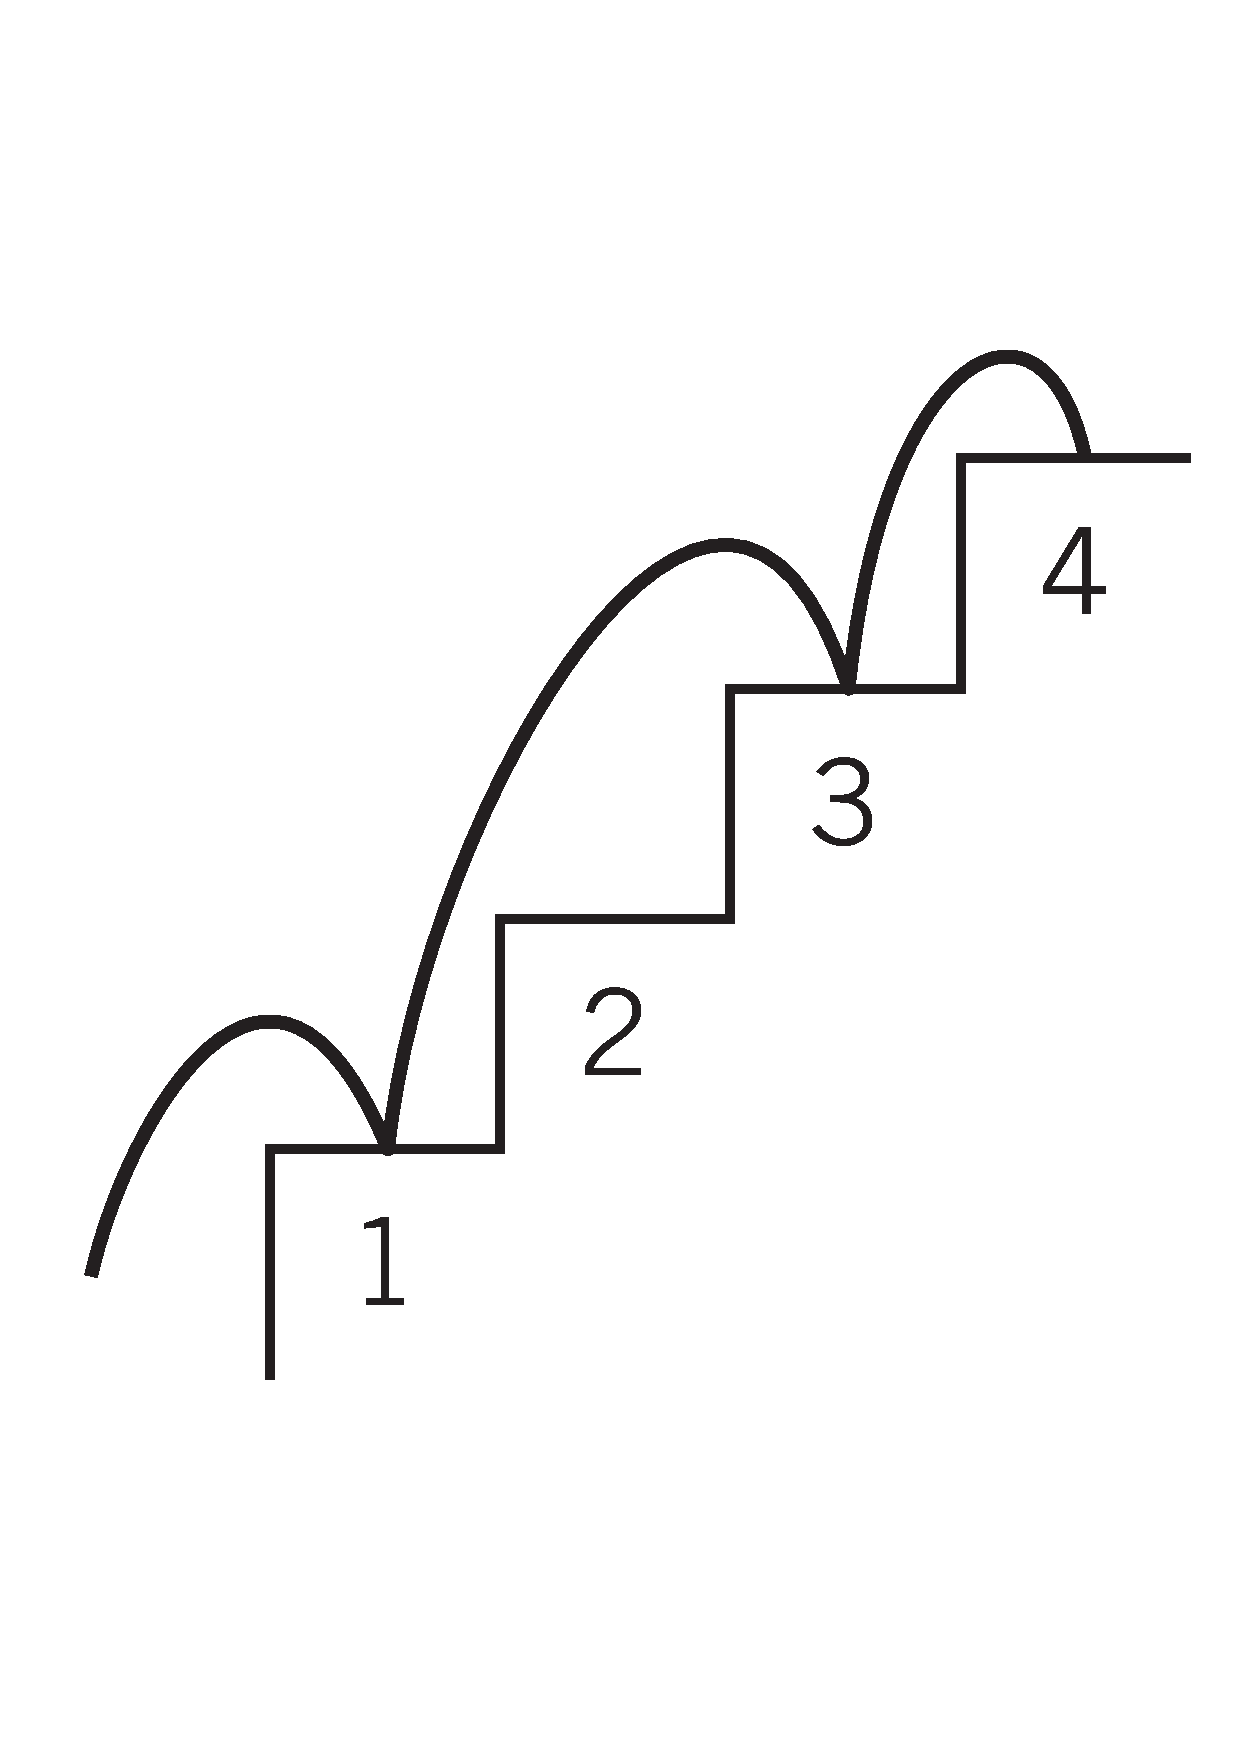
\includegraphics[width=0.8\linewidth]{Figures/stairs.pdf}
\end{minipage}
\end{exampleblock}
\noindent \textbf{Solución:}\\
Para $n = 1$ hay una única forma: dar un paso de un escalón.\\
Para $n = 2$ hay dos formas:
\begin{itemize}
\item dar dos pasos de un escalón,
\item dar un solo paso de dos escalones.
\end{itemize}
Para ver de cuántas maneras se puede subir una escalera de $n\geq 3$ escalones hacemos un análisis de casos:
\begin{itemize}
\item Si el primer paso es de un escalón, restan $n-1$: hay $a_{n-1}$ formas de completarlo.
\item Si el primer paso es de dos escalones, restan $n-2$: hay $a_{n-2}$ formas.
\end{itemize}
Por la regla de la suma:
\begin{equation}
a_n = a_{n-1} + a_{n-2} \quad \text{para } n \geq 3
\end{equation}
Resumiendo, tenemos la siguiente relación de recurrencia para calcular el número de formas $a_n$ en las que Juan puede subir una escalera de $n$ escalones:
\begin{align*}
  a_1 &~=~ 1\\
  a_2 &~=~ 2\\
  a_n &~=~ a_{n-1} + a_{n-2} \quad \forall n\geq 3
\end{align*}
Esta es la \textbf{sucesión de Fibonacci}, y tiene
muchas aplicaciones en problemas de conteo.



\begin{exampleblock}{Ejercicios: Palabras binarias sin 00 consecutivos}
Sea $a_n$ el número de palabras binarias de largo $n$ sin dos 
\end{exampleblock}
\noindent \textbf{Solución:}\\
Para construir una palabra binaria válida de largo $n$ (es decir, sin ocurrencias de $00$), consideramos los posibles caracteres finales:
\begin{itemize}
  \item Si la palabra termina en \texttt{1}, entonces el prefijo de largo $n - 1$ puede ser cualquier palabra válida. Hay $a_{n-1}$ de estas.
  \item Si termina en \texttt{0}, entonces el penúltimo carácter debe ser \texttt{1} (para evitar $00$). Por lo tanto, el prefijo de largo $n - 2$ puede ser cualquier palabra válida, seguida de \texttt{10}. Hay $a_{n-2}$ de estas.
\end{itemize}
Por la regla de la suma:
\[ a_n = a_{n-1} + a_{n-2} \quad \forall n\geq 3 \]
Condiciones iniciales:
\begin{align*}
a_1 &~=~ 2 \quad (\texttt{0}, \texttt{1}) \\
a_2 &~=~ 3 \quad (\texttt{01}, \texttt{10}, \texttt{11})
\end{align*}
Esta es nuevamente la \textbf{sucesión de Fibonacci}, pero con condiciones iniciales distintas.



\begin{exampleblock}{Ejercicio: Conexiones entre personas}
Cada vez que una nueva persona entra a una reunión, saluda a todas las personas que ya están. ¿Cuántos apretones de manos se han dado después de que han llegado $n$ personas (una por una)?
\end{exampleblock}
\noindent \textbf{Solución:}\\
Sea $a_n$ el número total de apretones de manos después de que han llegado $n$ personas. Cada nueva persona saluda a todas las que ya llegaron, es decir, realiza $n-1$ apretones. Entonces:
\begin{align*}
a_1 &= 0 \\
a_n &= a_{n-1} + (n - 1) \quad \text{para } n \geq 2
\end{align*}
% \noindent Esta secuencia representa los números triangulares desplazados.


% Ejercicio propuesto: Regiones en el plano
% Dibujando $n$ rectas con intersecciones generales, sea $a_n$ el número de regiones:
% % \begin{align*}
% % a_1 &= 2 \
% % a_n &= a_{n-1} + n \quad (n \geq 2)
% % \end{align*}




\begin{exampleblock}{Problema: Torres de Hanoi}
\noindent
\begin{minipage}[c]{0.74\textwidth}
\vspace*{0pt}
\centering
Las Torres de Hanoi son un puzzle que
consiste de 3 barras montadas en un tablero y una serie de discos de diferente tamaño.  
Inicialmente los discos estás dispuestos como se muestran a continuación:
El objetivo del puzzle es pasar todos los discos a otra de las barras con las siguientes restricciones:
\begin{itemize}
\item Los discos deben quedar dispuestos de la misma manera (en orden)
  %
\item Los discos se pueden pasar entre las barras, de a uno (por lo
  que en cada paso se puede mover sólo el disco superior de cada barra) 
  %
\item Al depositar un disco en otra barra, no puede quedar sobre otro de menor tamaño.
\end{itemize}
 ¿Cuál es la menor cantidad de movimientos $h_n$ que debo hacer para resolver el puzzle desde una configuración inicial con $n$ discos?
\end{minipage}%
\hfill
\begin{minipage}[c]{0.24\textwidth}
\centering
 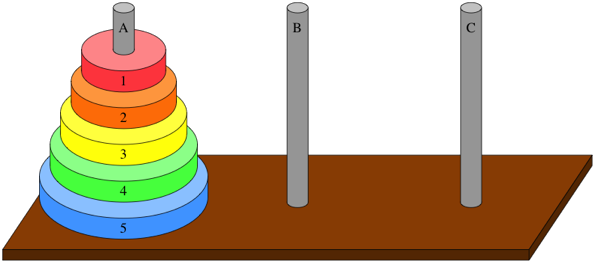
\includegraphics[width=\textwidth]{Figures/HanoiStarting.png}\hspace{1cm}
\end{minipage}
\end{exampleblock}
\noindent \textbf{Solución:}\\
La clave está en observar la estructura recursiva del problema.

\begin{itemize}
\item Para mover una torre de $n$ discos desde la barra origen a la barra destino:
\begin{enumerate}
\item Primero movemos los $n-1$ discos superiores a la barra auxiliar (requiere $h_{n-1}$ movimientos).
\item Luego movemos el disco más grande directamente a la barra destino (1 movimiento).
\item Finalmente, movemos los $n-1$ discos desde la barra auxiliar a la barra destino (otros $h_{n-1}$ movimientos).
\end{enumerate}
\end{itemize}

Esto da lugar a la siguiente relación de recurrencia:
\begin{align*}
  h_n &~=~ 2h_{n-1} + 1 \quad \forall n\geq 2 \\
  h_1 &~=~1 
\end{align*}
\medskip

Puede verificarse fácilmente que $$ h_n~=~2^n-1 $$ es la forma cerrada(o solución) de la recurrencia. 

\begin{exampleblock}{Asociación de productos (Números de Catalán)}
Sea $c_n$ el número de formas de parentizar $n$ factores $a_1 \cdot a_2 \cdot \cdots \cdot a_{n-1} \cdot a_n$. Demostrar la siguiente recurrencia:
\begin{align*}
c_1 &= 1 \\
c_n &= \sum_{i=1}^{n-1} c_i \cdot c_{n-i} \quad (n \geq 2)
\end{align*}
\end{exampleblock}
\noindent \textbf{Solución:}\\
Si se agrupa el producto como $(A) \cdot (B)$, donde:
\begin{itemize}
\item $A$ es un subproducto de los primeros $k$ factores,
\item $B$ es el subproducto de los $n-k$ restantes,
\end{itemize}
\noindent entonces hay $c_k$ formas de parentizar $A$ y $c_{n-k}$ formas de parentizar $B$, lo que da $c_k \cdot c_{n-k}$ formas para esa partición. Sumando sobre todas las posibles particiones (de $k = 1$ a $n-1$) obtenemos la recurrencia.

Esta sucesión es conocida como los \textbf{números de Catalán}, denotados habitualmente por $C_{n-1}$.
\textbf{Fórmula cerrada:}
\[
c_n = \frac{1}{n} \binom{2n - 2}{n - 1} = \frac{(2n - 2)!}{n!(n - 1)!}
\]

\subsection{Sistemas de relaciones de recurrencia}
En muchos problemas de conteo, la cantidad total de soluciones no depende solamente de un valor anterior en la secuencia, sino que involucra el resultado de varias secuencias interrelacionadas. En estos casos, hablamos de 	\textbf{sistemas de relaciones de recurrencia}. A diferencia de las relaciones simples, estos sistemas describen conjuntos de secuencias que se definen mutuamente.

\begin{exampleblock}{Ejercicio: Piezas de dominó y cuadrículas}
\textbf{Enunciado:} ¿De cuántas maneras, $F_n$, se puede llenar una cuadrícula de $3 \times n$ con piezas de dominó de $2 \times 1$?
\end{exampleblock}
\noindent \textbf{Solución:}\\
Para determinar $F_n$ analizamos cómo puede completarse la \textit{última columna} de la cuadrícula. Hay tres configuraciones típicas (ver Figura~\ref{fig:cuadricula_1}):
\begin{figure}[h]
\centering
\begin{tikzpicture}[scale=0.6]

% === Diagrama 1 ===
\begin{scope}[shift={(0,0)}]
  % grid
  \foreach \x in {0,...,6} {
    \draw (\x, 0) -- (\x, 3);
  }
  \foreach \y in {0,...,3} {
    \draw (4,\y) -- (6,\y); % final columns
  }
  \foreach \y in {0,...,3} {
    \draw (0,\y) -- (6,\y);
  }
  % Labels
  \node at (0.5,3.2) {\scriptsize 1};
  \node at (1.5,3.2) {\scriptsize 2};
  \node at (2.5,3.2) {\scriptsize 3};
  \node at (3.5,3.2) {\scriptsize $\cdots$};
  \node at (4.5,3.2) {\scriptsize $n{-}1$};
  \node at (5.5,3.2) {\scriptsize $n$};

  \node[anchor=east] at (0,2.5) {\tiny 1};
  \node[anchor=east] at (0,1.5) {\tiny 2};
  \node[anchor=east] at (0,0.5) {\tiny 3};

  % Highlight rectangles
  \draw[thick,blue] (0,0) rectangle (4,3);
  \fill[red!30,opacity=0.6] (4,2) rectangle (6,3);
  \fill[green!30,opacity=0.6] (4,1) rectangle (6,2);
  \fill[cyan!30,opacity=0.6] (4,0) rectangle (6,1);
\end{scope}

% === Diagrama 2 ===
\begin{scope}[shift={(8,0)}]
  % grid
  \foreach \x in {0,...,6} {
    \draw (\x, 0) -- (\x, 3);
  }
  \foreach \y in {0,...,3} {
    \draw (4,\y) -- (6,\y);
  }
  \foreach \y in {0,...,3} {
    \draw (0,\y) -- (6,\y);
  }

  % Labels
  \node at (0.5,3.2) {\scriptsize 1};
  \node at (1.5,3.2) {\scriptsize 2};
  \node at (2.5,3.2) {\scriptsize 3};
  \node at (3.5,3.2) {\scriptsize $\cdots$};
  \node at (4.5,3.2) {\scriptsize $n{-}1$};
  \node at (5.5,3.2) {\scriptsize $n$};

  \node[anchor=east] at (0,2.5) {\tiny 1};
  \node[anchor=east] at (0,1.5) {\tiny 2};
  \node[anchor=east] at (0,0.5) {\tiny 3};

  % Highlight rectangles
  
  \fill[red!30,opacity=0.6] (5,0) rectangle (6,2);
  \fill[green!30,opacity=0.6] (5,2) rectangle (6,3);
   \fill[green!30,opacity=0.6] (4,2) rectangle (5,3);
\end{scope}

% === Diagrama 3 ===
\begin{scope}[shift={(16,0)}]
  % grid
  \foreach \x in {0,...,6} {
    \draw (\x, 0) -- (\x, 3);
  }
  \foreach \y in {0,...,3} {
    \draw (4,\y) -- (6,\y);
  }
  \foreach \y in {0,...,3} {
    \draw (0,\y) -- (6,\y);
  }

  % Labels
  \node at (0.5,3.2) {\scriptsize 1};
  \node at (1.5,3.2) {\scriptsize 2};
  \node at (2.5,3.2) {\scriptsize 3};
  \node at (3.5,3.2) {\scriptsize $\cdots$};
  \node at (4.5,3.2) {\scriptsize $n{-}1$};
  \node at (5.5,3.2) {\scriptsize $n$};

  \node[anchor=east] at (0,2.5) {\tiny 1};
  \node[anchor=east] at (0,1.5) {\tiny 2};
  \node[anchor=east] at (0,0.5) {\tiny 3};

  % Highlight rectangles
  % \draw[thick,blue] (0,0) rectangle (5,3);
  \fill[red!30,opacity=0.6] (5,2) rectangle (6,3);
  \fill[red!30,opacity=0.6] (5,1) rectangle (6,2);
  \fill[green!30,opacity=0.6] (4,0) rectangle (6,1);
\end{scope}

\end{tikzpicture}
\caption{Tres formas posibles de completar la última columna de una cuadrícula $3 \times n$ usando piezas de dominó.}
\label{fig:cuadricula_1}
\end{figure}

Notar que la cantidad de maneras de llenar la cuadrícula en los últimos dos casos es la misma, ya que son simétricas. Llamemos $G_{n-1}$ a ese
número.  Luego, por la regla de la suma tenemos que
\[
F_n ~=~F_{n-2} + 2 G_{n-1}
\]

Nuevamente, hacemos análisis de casos sobre cómo puede rellenarse la columna más
pequeña de $G_{n}$. Vemos que hay dos maneras (ver Figura~\ref{fig:cuadricula_1}). En el primer caso, la forma de cubrir la subestructura es equivalente a $F_{n-1}$ y en el segundo caso, a $G_{n-2}$. Por lo tanto:
y por la regla de la suma resulta que
\[
  G_n ~=~ F_{n-1} + G_{n-2}
  \]
\begin{figure}[h]
\begin{center}
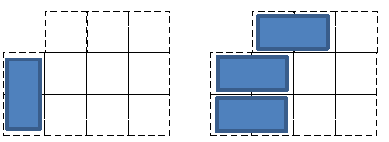
\includegraphics[width=0.4\textwidth]{Figures/tilingpattercases.png}  
\caption{Dos formas posibles de completar la última columna de una cuadrícula $G_{n}$ usando piezas de dominó.}
\label{fig:cuadricula_1}
\end{center}
\end{figure}
 Agregando las condiciones iniciales tenemos que
  \begin{align*}
    F_n &~=~F_{n-2} + 2 G_{n-1} \quad \forall n \geq 2\\
    F_0&~=~1\qquad F_1~=~0\\  
    G_n &~=~ F_{n-1} + G_{n-2}  \quad \forall n \geq 2\\
    G_0&~=~0\qquad G_1~=~1\\  
  \end{align*}
  lo que nos da un sistema de recurrencias para definir $F_n$. 


\subsection{Ejercicios propuestos}

\begin{itemize}
\item \textbf{Ejercicio:} Un string de números decimales es válido si contiene un número par de ceros. Use una relación de recurrencia para definir $c_n$, el número de strings válidos de largo $n$.
\medskip
\item \textbf{Ejercicio:} Defina recursivamente la sucesión ${a_n}$ que da la cantidad de strings de largo $n$ que no tienen dos ceros consecutivos.
\item \textbf{Ejercicio:} Supongamos que dibujamos $n$ rectas en una hoja de papel de manera que todo par de líneas se intersectan (pero no hay tres líneas que se intersectan en un único punto). ¿En cuántas regiones queda dividido el plano?
\end{itemize}
% \title{Apunte de Matemáticas Discretas CC3101:\\ 
% Soluciones de relaciones de recurrencia  Clase 14}
% % \title{Ejercicios Lógica e Inducción}
% \author{Andrés Abeliuk}
% \date{}
% \maketitle



\section{Recurrencias Lineales}

\subsection{Definición General}

\begin{definitionblock}{Recurrencia lineal homogénea con coeficientes constantes}
Una relación de recurrencia es \textbf{lineal, homogénea y con coeficientes constantes} si tiene la forma:
\[
a_n = c_1 a_{n-1} + c_2 a_{n-2} + \cdots + c_k a_{n-k},
\]
donde $c_1, c_2, \dots, c_k \in \mathbb{R}$ y $c_k \neq 0$. Decimos que la recurrencia es de \textbf{grado $k$}.
\end{definitionblock}

\begin{exampleblock}{Ejemplos}
\begin{itemize}
    \item $a_n = 3a_{n-1} + 2a_{n-3}$ es una recurrencia lineal, homogénea, con coeficientes constantes, de grado $3$.
    \item $a_n = a_{n-1}^2$ \textbf{no} es lineal.
    \item $a_n = a_{n-1} + 1$ \textbf{no} es homogénea.
    \item $a_n = n a_{n-1}$ \textbf{no} tiene coeficientes constantes.
\end{itemize}
\end{exampleblock}

\subsection{Estrategia de Resolución}

La idea central para resolver estas recurrencias es asumir que las soluciones tienen la forma $a_n = r^n$. Sustituyendo esta forma en la ecuación de recurrencia se obtiene la llamada \textbf{ecuación característica}:

\begin{align*}
 &  r^n = c_1 r^{n-1} + c_2 r^{n-2} + \cdots + c_k r^{n-k} \\
& \hspace{-3ex} \Leftrightarrow\\
&  r^k = c_1 r^{k-1} + c_2 r^{k-2} + \cdots + c_k
\end{align*}

Resolver esta ecuación polinomial nos da las raíces $r_i$, y la solución general de la recurrencia se construye a partir de estas raíces, dependiendo de su multiplicidad.

\subsubsection{Caso de Grado 2 con Raíces Distintas}

\begin{thmblock}{Solución con raíces distintas}
Sea la recurrencia:
\[
a_n = c_1 a_{n-1} + c_2 a_{n-2}
\]
y supongamos que la ecuación característica $r^2 = c_1 r + c_2$ tiene dos raíces reales distintas $r_1$ y $r_2$. Entonces, la solución general es:
\[
a_n = \alpha_1 r_1^n + \alpha_2 r_2^n,
\]
donde $\alpha_1$ y $\alpha_2$ se determinan usando las condiciones iniciales.
\end{thmblock}
\begin{proof}
Por hipótesis, sabemos que $r_1^2 = c_1 r_1 + c_2$ y $r_2^2 = c_1 r_2 + c_2$. Entonces:
\begin{align*}
c_1 a_{n-1} + c_2 a_{n-2} &= c_1(\alpha_1 r_1^{n-1} + \alpha_2 r_2^{n-1}) + c_2(\alpha_1 r_1^{n-2} + \alpha_2 r_2^{n-2}) \\
&= \alpha_1 r_1^{n-2}(c_1 r_1 + c_2) + \alpha_2 r_2^{n-2}(c_1 r_2 + c_2) \\
&= \alpha_1 r_1^n + \alpha_2 r_2^n \\
&= a_n
\end{align*}
Concluimos que $a_n = \alpha_1 r_1^n + \alpha_2 r_2^n$ es solución para cualquier par de constantes $\alpha_1, \alpha_2$.

Si además se conocen las condiciones iniciales $a_0$ y $a_1$, entonces las constantes $\alpha_1, \alpha_2$ se determinan unívocamente resolviendo el sistema lineal:
\[
\begin{cases}
a_0 = \alpha_1 r_1^0 + \alpha_2 r_2^0 \\
a_1 = \alpha_1 r_1^1 + \alpha_2 r_2^1
\end{cases}
\]
\end{proof}

\begin{exampleblock}{Ejemplo}
Considere la relación de recurrencia,
\[
\begin{cases}
a_n = 2a_{n-1} + 3a_{n-2}, \quad \text{para } n \geq 2 \\
a_0 = a_1 = 1
\end{cases}
\]
La ecuación característica es $r^2 = 2r + 3 \Rightarrow r^2 - 2r - 3 = 0$, con raíces $r_1 = 3$, $r_2 = -1$.

Solución general:
\[
a_n = \alpha_1 3^n + \alpha_2 (-1)^n
\]
Usamos condiciones iniciales para determinar:
\[
\begin{cases}
1 = \alpha_1 + \alpha_2 \\
1 = 3\alpha_1 - \alpha_2
\end{cases}
\Rightarrow \alpha_1 = \frac{1}{2}, \quad \alpha_2 = \frac{1}{2}
\]
Solución final:
\[
a_n = \tfrac{1}{2} 3^n + \tfrac{1}{2} (-1)^n
\]
\end{exampleblock}

\subsection{Raíces Dobles}

\begin{thmblock}{Solución con raíz doble}
Si la ecuación característica tiene una raíz doble $r_*$, es decir, $r^2 = c_1 r + c_2$ con $r_1 = r_2 = r_*$, entonces la solución general es:
\[
a_n = \alpha_1 r_*^n + \alpha_2 n r_*^n.
\]
\end{thmblock}
\begin{proof}
Por hipótesis, sabemos que $r_*^2 = c_1 r_* + c_2$. Por lo tanto:
\begin{align*}
c_1 a_{n-1} + c_2 a_{n-2} &= c_1(\alpha_1 r_*^{n-1} + \alpha_2 (n-1) r_*^{n-1}) + c_2(\alpha_1 r_*^{n-2} + \alpha_2 (n-2) r_*^{n-2}) \\
&= \alpha_1 r_*^{n-2} (c_1 r_* + c_2) + \alpha_2 r_*^{n-2} ((n-1) c_1 r_* + (n-2) c_2) \\
&= \alpha_1 r_*^n + \alpha_2 r_*^{n-2} (n c_1 r_* - c_1 r_* + n c_2 - 2 c_2) \\
&= \alpha_1 r_*^n + \alpha_2 r_*^{n-2} (n(c_1 r_* + c_2) - c_1 r_* - 2c_2) \\
&= \alpha_1 r_*^n + \alpha_2 n r_*^n - \alpha_2 r_*^{n-2}(c_1 r_* + 2c_2) \\
&= a_n - \alpha_2 r_*^{n-2}(c_1 r_* + 2c_2)
\end{align*}
Para que la expresión sea igual a $a_n$, basta establecer que $c_1 r_* + 2c_2 = 0$.

\noindent \textit{Nota:} Como $r_*$ es raíz doble, esto significa que la ecuación característica
\[
r^2 - c_1 r - c_2 = 0
\]
tiene un discriminante nulo:
\[
\Delta = c_1^2 + 4c_2 = 0.
\]
Aplicando la fórmula general de las raíces cuadráticas:
\[
r = \frac{c_1 \pm \sqrt{c_1^2 + 4c_2}}{2},
\]
obtenemos que:
\[
r_* = \frac{c_1}{2}
\]
cuando el discriminante es cero. Reemplazando en $c_1 r_* + 2c_2$ se obtiene:
\[
c_1 r_* + 2c_2 = \frac{c_1^2}{2} + 2c_2 = 2\Delta =  0,
\]
por lo tanto, se verifica la igualdad y concluimos que
\[
a_n = \alpha_1 r_*^n + \alpha_2 n r_*^n
\]
es solución para cualquier par de constantes $\alpha_1, \alpha_2$.
\end{proof}


\subsection{Caso General: Grado Arbitrario}

\begin{thmblock}{Solución general de grado $k$}
Sea
\[
a_n = c_1 a_{n-1} + \cdots + c_k a_{n-k}
\]
una recurrencia con ecuación característica que tiene $t$ raíces distintas $r_1, \dots, r_t$ con multiplicidades $m_1, \dots, m_t$. Entonces, la solución general es:

\[
a_n = \sum_{i=1}^t \left( \sum_{j=0}^{m_i - 1} \alpha_{i,j} n^j \right) r_i^n
\]
\end{thmblock}

% \subsection*{Ejercicio: Recurrencias simultáneas}
% \noindent Resuelva el siguiente sistema de recurrencias:
% \[
% \begin{cases}
% a_n = 3 a_{n-1} + 2 b_{n-1} \\
% b_n = a_{n-1} + 2 b_{n-1} \\
% a_0 = 1,\ b_0 = 2
% \end{cases}
% \]
% \textbf{Paso 1:} Resolvamos la segunda ecuación. Se puede reescribir como una recurrencia lineal para $b_n$:
% \[
% b_n = a_{n-1} + 2b_{n-1}.
% \]
% Pero aún depende de $a_{n-1}$, así que intentemos eliminar $a_n$ utilizando la diferencia:
% Restamos la primera y la segunda ecuación:
% \[
% a_n - b_n = 2(a_{n-1} - b_{n-1})
% \]
% Definamos $d_n = a_n - b_n$. Entonces:
% \[
% d_n = 2 d_{n-1}, \quad d_0 = a_0 - b_0 = 1 - 2 = -1.
% \]
% Esto nos da:
% \[
% d_n = -1 \cdot 2^n = -2^n.
% \]
% Ahora usamos que $a_n = b_n + d_n = b_n - 2^n$ en la ecuación de $b_n$:
% \[
% b_n = a_{n-1} + 2 b_{n-1} = (b_{n-1} - 2^{n-1}) + 2 b_{n-1} = 3b_{n-1} - 2^{n-1}
% \]
% Entonces $b_n$ cumple:
% \[
% b_n = 3b_{n-1} - 2^{n-1}, \quad b_0 = 2.
% \]
% Esta es una recurrencia no homogénea. Propongamos una solución particular de la forma $A 2^n$. Probamos:
% \[
% A 2^n = 3A 2^{n-1} - 2^{n-1} \Rightarrow A 2^n = (3A - 1) 2^{n-1} \Rightarrow A = 3A - 1 \Rightarrow A = \frac{1}{2}.
% \]
% Solución particular: $b_n^{(p)} = \frac{1}{2} 2^n$.\
% Solución general de la homogénea: $b_n^{(g)} = \alpha 3^n$.\
% Entonces:
% \[
% b_n = \alpha 3^n + \frac{1}{2} 2^n.
% \]
% Con $b_0 = 2$ obtenemos $\alpha = \frac{3}{2}$, así que:
% \[
% b_n = \frac{3}{2} 3^n + \frac{1}{2} 2^n.
% \]
% Finalmente, usamos que $a_n = b_n - 2^n$:
% \[
% a_n = \frac{3}{2} 3^n + \frac{1}{2} 2^n - 2^n = \frac{3}{2} 3^n - \frac{1}{2} 2^n.
% \]
% \textbf{Solución final:}
% \[
% \boxed{a_n = \frac{3}{2} 3^n - \frac{1}{2} 2^n, \quad b_n = \frac{3}{2} 3^n + \frac{1}{2} 2^n.}
% \]



\subsection{Recurrencias No Homogéneas}
\begin{definitionblock}{Recurrencia lineal no homogénea}
Una relación de recurrencia lineal, a coeficientes constantes de grado $k$, se dice \textbf{no homogénea} si es de la forma:
\[
a_n = c_1 a_{n-1} + c_2 a_{n-2} + \cdots + c_k a_{n-k} + f(n),
\]
donde $c_1, c_2, \dots, c_k$ son números reales, $c_k \neq 0$, y $f(n)$ es una función arbitraria. \\
Definimos la \textbf{recurrencia homogénea asociada}:
\[
a_n = c_1 a_{n-1} + c_2 a_{n-2} + \cdots + c_k a_{n-k}
\]
\end{definitionblock}

\begin{exampleblock}{Ejemplos}
\begin{itemize}
  \item $a_n = 2a_{n-1} + 1$ \hfill (no homogénea de grado 1)
  \item $a_n = 2a_{n-1} - 3a_{n-3} + 5n^2 + 2^n$ \hfill (no homogénea de grado 3)
\end{itemize}
\end{exampleblock}

\begin{thmblock}{Teorema de la solución general}
La solución general de una recurrencia no homogénea es:
\[
a_n = a_n^{(g)} + a_n^{(p)},
\]
donde $a_n^{(g)}$ es la solución general de la homogénea asociada, y $a_n^{(p)}$ es una solución particular de la no homogénea.
\end{thmblock}

% \noindent \textit{¿Qué es una solución particular?}\\
\noindent Una \textbf{solución particular} $a_n^{(p)}$ es una función concreta que satisface la relación de recurrencia completa, es decir, incluyendo el término no homogéneo $f(n)$. A diferencia de la solución general, que contiene constantes libres, una solución particular es un caso específico. Se utiliza como complemento a la solución general de la parte homogénea para construir la solución total.\\
Por ejemplo, si tenemos:
\[
a_n = 2a_{n-1} + 1,
\]
la recurrencia homogénea asociada es $a_n^{(g)} = \alpha 2^n$. Una solución particular válida es $a_n^{(p)} = -1$, ya que satisface:
\[
-1 = 2(-1) + 1.
\]
Entonces, la solución general completa es:
\[
a_n = \alpha 2^n - 1.
\]

\begin{proof}
Como $a_n^{(p)}$ es una solución particular de la relación de recurrencia no homogénea, se cumple que:
\[
a^{(p)}_n = c_1a^{(p)}_{n-1} + c_2a^{(p)}_{n-2} + \dots + c_ka^{(p)}_{n-k} + f(n)
\]
Supongamos ahora que $b_n$ es otra solución de la misma relación no homogénea, entonces también se cumple:
\[
b_n = c_1b_{n-1} + c_2b_{n-2} + \dots + c_kb_{n-k} + f(n)
\]
Restando ambas expresiones:
\[
b_n - a^{(p)}_n = c_1(b_{n-1} - a^{(p)}_{n-1}) + c_2(b_{n-2} - a^{(p)}_{n-2}) + \dots + c_k(b_{n-k} - a^{(p)}_{n-k})
\]
Esto implica que la diferencia $b_n - a_n^{(p)}$ satisface la relación de recurrencia homogénea asociada. Es decir, $b_n - a_n^{(p)} = a_n^{(g)}$ para alguna solución homogénea $a_n^{(g)}$.\
Por lo tanto:
\[
b_n = a_n^{(p)} + a_n^{(g)},
\]
como se quería demostrar.
\end{proof}

\begin{exampleblock}{Ejemplo: Torres de Hanoi}
La mínima cantidad de movimientos $h_n$ necesarios para resolver el problema de las Torres de Hanoi con $n$ discos satisface:
\[
\begin{cases}
h_1 = 1 \\
h_n = 2 h_{n-1} + 1 \quad (n \geq 2)
\end{cases}
\]

\textbf{Paso 1:} Se trata de una recurrencia no homogénea de primer orden con $f(n)=1$.

La recurrencia homogénea asociada es:
\[
h_n = 2 h_{n-1},
\]
cuyo comportamiento general es:
\[
h_n^{(g)} = \alpha 2^n.
\]

\textbf{Paso 2:} Buscamos una solución particular $h_n^{(p)}$ tal que:
\[
h_n^{(p)} = 2 h_{n-1}^{(p)} + 1.
\]
Probamos con una constante $h_n^{(p)} = C$:
\[
C = 2C + 1 \Rightarrow C = -1.
\]
Entonces, una solución particular es $h_n^{(p)} = -1$.

\textbf{Paso 3:} La solución general es:
\[
h_n = h_n^{(g)} + h_n^{(p)} = \alpha 2^n - 1.
\]
Usamos la condición inicial $h_1 = 1$:
\[
1 = \alpha 2^1 - 1 \Rightarrow 1 = 2\alpha - 1 \Rightarrow \alpha = 1.
\]

\textbf{Solución cerrada:}
\[
\boxed{h_n = 2^n - 1}
\]
\end{exampleblock}

\subsection{Soluciones Particulares: Método de coeficientes indeterminados}

Obtener la solución general $a_n^{(g)}$ de la recurrencia homogénea asociada es fácil (vimos cómo hacerlo).  Sin embargo no hay ningún mecanismo general para obtener una solución particular $a_n^{(p)}$ de una
recurrencia no homogénea. 
Para una clase particular de $f$'s tenemos el siguiente teorema:


\begin{thmblock}{Teorema}
Sea la recurrencia $a_n = c_1 a_{n-1} + c_2 a_{n-2} + \cdots + c_k a_{n-k} + f(n)$, donde
\[ f(n) = (b_t n^t + b_{t-1} n^{t-1} + \cdots + b_1 n + b_0) s^n, \]
y $b_0, b_1, \dots, b_t$ y $s$ son números reales. Entonces:

\begin{itemize}
  \item Si $s$ \textbf{no es raíz} de la ecuación característica asociada, entonces existe una solución particular de la forma:
  \[ (p_t n^t + p_{t-1} n^{t-1} + \cdots + p_1 n + p_0) s^n. \]

  \item Si $s$ \textbf{es raíz} de la ecuación característica con multiplicidad $m$, entonces existe una solución particular de la forma:
  \[ n^m (p_t n^t + p_{t-1} n^{t-1} + \cdots + p_1 n + p_0) s^n. \]

\end{itemize}
\end{thmblock}

\subsection*{Ejercicio resuelto}

\begin{exampleblock}{Ejercicio: recurrencia con término lineal}
Encuentre la solución general de la recurrencia:
\[
a_n = 3 a_{n-1} - 4n
\]
\end{exampleblock}

\noindent \textbf{Paso 1:} Estudiamos la recurrencia homogénea asociada:
\[
a_n^{(g)} = 3 a_{n-1}^{(g)} \Rightarrow a_n^{(g)} = \alpha 3^n
\]

\noindent \textbf{Paso 2:} Como el término no homogéneo es $f(n) = -4n$, un polinomio de grado 1, proponemos una solución particular de la forma:
\[
a_n^{(p)} = cn + d
\]
Sustituimos en la ecuación original:
\[
cn + d = 3(c(n-1) + d) - 4n
\]
Expandimos el lado derecho:
\[
cn + d = 3cn - 3c + 3d - 4n
\]
Agrupamos términos:
\[
cn + d = (3c - 4)n + (3d - 3c)
\]
Igualando coeficientes de ambos lados:
\[
\begin{cases}
c = 3c - 4 \\
d = 3d - 3c
\end{cases} \Rightarrow 
\begin{cases}
2c = 4 \Rightarrow c = 2 \\
3d - 3c = d \Rightarrow 2d = 3c \Rightarrow d = \frac{3c}{2} = 3
\end{cases}
\]

\noindent \textbf{Paso 3:} Por lo tanto, una solución particular es:
\[
a_n^{(p)} = 2n + 3
\]
\textbf{Solución general:}
\[
a_n = a_n^{(g)} + a_n^{(p)} = \alpha 3^n + 2n + 3
\]
\textbf{Nota:} Para determinar $\alpha$ se requiere una condición inicial adicional, como $a_0$ o $a_1$.


\subsection{Ejercicios Propuestos}

\begin{itemize}
    \item Resolver $a_n = a_{n-1} + 2a_{n-2}$, con $a_0 = 2$, $a_1 = 7$.
    \item Encontrar una fórmula explícita para los números de Fibonacci.
    % \item Hallar la solución de $a_n = 3 a_{n-1} - 4n$.
    \item Encontrar una solución particular para: $a_n = 6 a_{n-1} - 9 a_{n-2} + n 3^n$ y $a_n = 6 a_{n-1} - 9 a_{n-2} + (n^2 + 1) 2^n$.
    \item Defina una recurrencia $s_n$ para la suma de los primeros $n$ naturales, y resuélvala.
    \item Resolver el sistema:
    \[
    \begin{cases}
    a_n = 3a_{n-1} + 2b_{n-1} \\
    b_n = a_{n-1} + 2b_{n-1} \\
    a_0 = 1,\ b_0 = 2
    \end{cases}
    \]
\end{itemize}

% \title{Apunte de Matemáticas Discretas CC3101:\\ 
% Funciones Generadoras (Parte 1)  Clase 15}
% % \title{Ejercicios Lógica e Inducción}
% \author{Andrés Abeliuk}
% \date{}
% \maketitle


\section{Funciones Generadoras}
\subsection{Introducción}

En muchas ocasiones, necesitamos describir secuencias de números, por ejemplo, el número de formas de resolver un problema de conteo o los términos definidos por una relación de recurrencia. Existen varias formas de describir una secuencia:

\begin{itemize}
    \item Por extensión: listar los primeros términos, como $0, 1, 3, 7, 15, 31, \ldots$
    \item Por una relación de recurrencia: por ejemplo, $a_n = 2a_{n-1} + 1$
    \item Por una fórmula cerrada: como $a_n = 2^n - 1$
\end{itemize}

Sin embargo, existe una herramienta aún más poderosa: asociar a la secuencia una \emph{función generadora}, que encapsula toda la información de la secuencia en una única expresión formal. Las funciones generadoras no sólo permiten representar una secuencia, sino también manipularla algebraicamente para obtener nuevas propiedades y resolver recurrencias.

\subsection{Definición de Función Generadora}

\begin{definitionblock}{Función Generadora}
Sea $\{a_n\}_{n \geq 0}$ una secuencia de números reales o complejos. Su \textbf{función generadora ordinaria} (o simplemente función generadora) es la serie formal:
\[
A(x) = \sum_{n \geq 0} a_n x^n
\]
Aquí, $x$ se interpreta como un marcador formal, no como una variable real: lo que nos interesa no es el valor de la suma sino los coeficientes $a_n$.
\end{definitionblock}


\subsection{Ejemplos Iniciales}

\begin{exampleblock}{Ejemplo secuencia constante:}
La secuencia constante $a_n = 3$, para todo $n \geq 0$, tiene como función generadora:
\[
A(x) = \sum_{n \geq 0} 3x^n = 3(1 + x + x^2 + x^3 + \cdots)
\]
Pero puede escribirse en forma más sucinta: $A(x)$ es una \textbf{serie geométrica}, cuya suma conocemos si $|x| < 1$:
\[
A(x) = \frac{3}{1 - x}
\]
\end{exampleblock}

\begin{exampleblock}{Ejemplo secuencia lineal:}
Para $a_n = n+1$, tenemos:
\[
A(x) = \sum_{n \geq 0} (n+1)x^n = \frac{1}{(1 - x)^2}
\]
\end{exampleblock}



\begin{exampleblock}{Ejemplo secuencia exponencial:}
Para $a_n = c^n$, con $c$ constante:
\[
A(x) = \sum_{n \geq 0} (cx)^n = \frac{1}{1 - cx}
\]
\end{exampleblock}

\begin{exampleblock}{Ejemplo secuencia binomio:}
Para $a_n = \binom{m}{n}$ con $m$ fijo, entonces:
\[
A(x) = \sum_{n \geq 0} \binom{m}{n} x^n = (1 + x)^m
\]
\end{exampleblock}

\subsection{Resolución de Recurrencias}

Una de las principales aplicaciones de las funciones generadoras es resolver relaciones de recurrencia. Veremos cómo transformar una recurrencia en una expresión cerrada usando funciones generadoras.

\subsubsection*{Ejemplo}
Sea la secuencia definida recursivamente por $a_0 = 0$ y $a_{n+1} = 2a_n + 1$ para todo $n \geq 0$.

Queremos encontrar una forma cerrada para $a_n$. Para ello, multiplicamos ambos lados de la recurrencia por $x^n$:
\[
a_{n+1}x^n = 2a_n x^n + x^n
\]
y luego sumamos para todo $n \geq 0$:
\[
\sum_{n \geq 0} a_{n+1} x^n = \sum_{n \geq 0} (2a_n + 1)x^n
\]

En el lado izquierdo tenemos \emph{casi} $A(x)$, excepto por el \'indice $n+1$ en vez de $n$. Podemos re-armar $A(x)$ ``multiplicando y dividiendo por $x$'':
% El lado izquierdo se reescribe como:
\[
\sum_{n \geq 0} a_{n+1} x^n ={\frac{1}{x}\sum_{n\geq 0}{a_{n+1} x^{n+1}} }= \frac{A(x) - a_0}{x} = \frac{A(x)}{x}
\]
 En el lado derecho tenemos 
\begin{align*}
    \sum_{n\geq 0}{(2 a_n x^n + x^n)} &
    ~=~ 2\sum_{n\geq 0}{a_n x^n} + \sum_{n\geq 0}{x^n} 
    ~=~ 2 A(x) +\sum_{n\geq 0} x^n 
    ~=~ 2A(x) + \frac{1}{1-x}
\end{align*}     
donde usamos la forma cerrada para la serie geom\'etrica (v\'alida para 
   $|x|<1$, lo cual supondremos siempre en estas manipulaciones).\\
Igualando ambas expresiones:
\[
\frac{A(x)}{x} = 2A(x) + \frac{1}{1 - x}
\]
Despejando $A(x)$:
\[
A(x) = \frac{x}{(1 - x)(1 - 2x)}
\]

\begin{exampleblock}{¿Cómo seguimos?} Si podemos transformar $A(x)$ de vuelta en una serie tipo $\sum_{n\geq 0}{a_nx^n}$, basta con identificar el coeficiente de $x^n$ para obtener una fórmula explícita para $a_n$.
\end{exampleblock}

Para ello, realizamos una expansión en fracciones parciales. Notamos que:
\[
\frac{x}{(1 - x)(1 - 2x)} = x\left(\frac{2}{1 - 2x} - \frac{1}{1 - x}\right)
\]
Y sabemos las series que representan las dos fracciones de la derecha:
\[
x \cdot \left(\frac{2}{1 - 2x}\right) - x \cdot \left(\frac{1}{1 - x}\right) = 2x \cdot \sum_{n\geq 0}(2x)^n - x \cdot \sum_{n\geq 0} x^n
\]
% Recordando que $\sum_{n\geq 0} x^n = \frac{1}{1 - x}$ para $|x| < 1$, 
Obtenemos:
\[
2x \cdot \sum_{n\geq 0}(2^n x^n) = \sum_{n\geq 0} 2^{n+1} x^{n+1} = \sum_{n\geq 1} 2^n x^n
\]
\[
x \cdot \sum_{n\geq 0} x^n = \sum_{n\geq 0} x^{n+1} = \sum_{n\geq 1} x^n
\]

Restando las dos series:
\[
\sum_{n\geq 1}(2^n - 1) x^n = \sum_{n\geq 0}(2^n - 1)x^n - (2^0 - 1) = \sum_{n\geq 0}(2^n - 1)x^n
\]

Por lo tanto, \textbf{la solución de la recurrencia es}:
\[
a_n = 2^n - 1
\]


\subsection{Resolución de recurrencias: Receta General}
La técnica de funciones generadoras es especialmente útil para resolver relaciones de recurrencia y obtener formas cerradas de sus soluciones. A continuación presentamos una receta paso a paso que resume el proceso:

\begin{enumerate}
  \item \textbf{Transformar la relación de recurrencia en una función generadora:}
  \begin{enumerate}[label=\alph*)]
    \item Asegúrese de que la recurrencia esté bien definida, incluyendo condiciones iniciales claras y los valores de $n$ para los cuales se aplica.
    \item Dé un nombre a la función generadora: por ejemplo, $A(x) = \sum_{n \geq 0} a_n x^n$.
    \item Multiplique ambos lados de la relación por $x^n$.
    \item Sume ambos lados para todos los valores de $n$ donde la relación es válida.
    \item Exprese los resultados en términos de la función generadora $A(x)$.
    \item Despeje $A(x)$.
  \end{enumerate}

  \item \textbf{Transformar $A(x)$ en una serie de potencias:}
  \begin{enumerate}[label=\alph*)]
    \item Si $A(x)$ es una función racional (es decir, cociente entre dos polinomios), intente expandirla mediante \emph{fracciones parciales}.
    \item Utilice identidades conocidas de series geométricas para reescribir cada término como una serie de potencias.
  \end{enumerate}

  \item \textbf{Leer la solución:}
  \begin{enumerate}[label=\alph*)]
    \item Identifique el coeficiente de $x^n$ en la expansión final: eso corresponde al valor de $a_n$ en forma cerrada.
  \end{enumerate}
\end{enumerate}

Este procedimiento ha sido ilustrado en el ejemplo del caso $a_{n+1} = 2a_n + 1$, donde finalmente llegamos a la forma cerrada $a_n = 2^n - 1$ a través de funciones generadoras.

\subsection{Propiedades y ejemplos clásicos de funciones generadoras}

Las funciones generadoras no solo sirven para resolver recurrencias, sino que también poseen propiedades algebraicas que facilitan su manipulación y permiten construir nuevas funciones a partir de otras ya conocidas. En esta sección reunimos varios resultados útiles y ejemplos clásicos.

\subsubsection{Operaciones básicas entre funciones generadoras}

\begin{thmblock}{Teorema (Serie de Potencias)}
Si $A(x) = \sum_{n\geq 0} a_n x^n$ y $B(x) = \sum_{n\geq 0} b_n x^n$ son funciones generadoras y ambas series convergen, entonces:

\begin{itemize}
  \item Suma:
  \[
  A(x) + B(x) = \sum_{n\geq 0} (a_n + b_n) x^n
  \]

  \item Producto (convolución):
  \[
  A(x) \cdot B(x) = \sum_{n\geq 0} \left(\sum_{k=0}^{n} a_k b_{n-k} \right) x^n
  \]
  Esta operación se conoce como \emph{convolución}.
\end{itemize}
\end{thmblock}

\begin{exampleblock}{Ejemplo: convolución de series geométricas}
Sea $A(x)=\frac{1}{(1 - x)^2}$ una función generadora.
Queremos obtener su expansión como serie de potencias.

Primero, recordemos que:
\[
\frac{1}{1 - x} = \sum_{n\geq 0} x^n
\]

Multiplicando dos veces esta serie:
\[
\left(\frac{1}{1 - x}\right)^2 = \left(\sum_{n\geq 0} x^n\right)^2 = \sum_{n\geq 0} (n + 1) x^n
\]

Esto corresponde a la función generadora de la secuencia $1, 2, 3, 4, \dots$.
\end{exampleblock}

\subsection{Catálogo clásico de funciones generadoras}

\begin{center}
\def\arraystretch{1.3}
\begin{tabular}{l|c|c}
\hline
\textbf{Secuencia} & \textbf{Función Generadora} & \textbf{Forma cerrada} \\
\hline\hline
$1, 0, 0, 0, \ldots$ & $\sum_{n\geq 0} [n = 0] x^n$ & $1$ \\
$1, 1, 1, 1, \ldots$ & $\sum_{n\geq 0} x^n$ & $\frac{1}{1 - x}$ \\
$1, -1, 1, -1, \ldots$ & $\sum_{n\geq 0} (-1)^n x^n$ & $\frac{1}{1 + x}$ \\
$1, c, c^2, c^3, \ldots$ & $\sum_{n\geq 0} c^n x^n$ & $\frac{1}{1 - cx}$ \\
$1, 2, 3, 4, \ldots$ & $\sum_{n\geq 0} (n + 1) x^n$ & $\frac{1}{(1 - x)^2}$ \\
$\binom{c}{0}, \binom{c}{1}, \ldots$ & $\sum_{n\geq 0} \binom{c}{n} x^n$ & $(1 + x)^c$ \\
$\binom{c - 1}{0}, \binom{c}{1}, \ldots$ & $\sum_{n\geq 0} \binom{c + n - 1}{n} x^n$ & $\frac{1}{(1 - x)^c}$ \\
\hline
\end{tabular}
\end{center}

Estas funciones generadoras permiten reconocer patrones y resolver rápidamente problemas de conteo o recurrencias.

\bigskip

\subsection{Ejemplo: sucesión de Fibonacci}
\noindent \textbf{Paso 1.} A partir de la relación de recurrencia $F_{n+1} = F_n + F_{n-1}$, con $F_0 = 0$ y $F_1 = 1$, queremos obtener la función generadora $F(x) = \sum_{n \geq 0} F_n x^n$.

\noindent Multiplicamos ambos lados por $x^n$ y sumamos desde $n = 1$:
\[
\sum_{n \geq 1} F_{n+1} x^n = \sum_{n \geq 1} F_n x^n + \sum_{n \geq 1} F_{n-1} x^n
\]
El lado izquierdo se transforma en:
\[
\sum_{n \geq 1} F_{n+1} x^n = \frac{1}{x}(F(x) - x)
\]
El lado derecho:
\[
\sum_{n \geq 1} F_n x^n + \sum_{n \geq 1} F_{n-1} x^n = F(x) + xF(x)
\]
Igualando ambos lados:
\[
\frac{1}{x}(F(x) - x) = F(x) + xF(x)
\]
Despejando:
\[
F(x) = \frac{x}{1 - x - x^2}
\]

\noindent \textbf{Paso 2.} Recuperamos la serie de potencias de:
\[
F(x) = \frac{x}{1 - x - x^2}
\]
Esto puede hacerse mediante fracciones parciales. Para ello factorizamos el denominador:
\[
1 - x - x^2 = (1 - r_0 x)(1 - r_1 x)
\]
donde $r_0 = \frac{1 + \sqrt{5}}{2}$ y $r_1 = \frac{1 - \sqrt{5}}{2}$.
Así:
\[
F(x) = \frac{x}{(1 - r_0 x)(1 - r_1 x)} = \frac{1}{r_0 - r_1} \left(\frac{1}{1 - r_0 x} - \frac{1}{1 - r_1 x}\right)
\]
Como sabemos que:
\[
\frac{1}{1 - ax} = \sum_{n \geq 0} a^n x^n
\]
Podemos escribir:
\[
F(x) = \sum_{n \geq 0} \frac{1}{\sqrt{5}} (r_0^n - r_1^n) x^n
\]
Por lo tanto,
\[
F_n = \frac{1}{\sqrt{5}} (r_0^n - r_1^n)
\]
Esta es la conocida fórmula cerrada de los números de Fibonacci, también llamada fórmula de Binet.

\section*{Referencias}
\textbf{Libros de referencia:}
\begin{itemize}
  \item ``Concrete Mathematics'' de R.~Graham, D.~Knuth, y O.~Patashnik.
\end{itemize}

% \title{Apunte de Matemáticas Discretas CC3101:\\ 
% Funciones Generadoras (Parte 2)  Clase 16}
% % \title{Ejercicios Lógica e Inducción}
% \author{Andrés Abeliuk}
% \date{}
% \maketitle


\section{Más sobre funciones generadoras}

\subsection{Coeficientes Binomiales}
Las funciones generadoras no solo sirven para encontrar soluciones cerradas a recurrencias, sino que también son \emph{herramientas poderosas para resolver problemas de conteo sofisticados}. Para esto, necesitamos extender la noción de coeficientes binomiales a casos más generales.

A continuación definimos los coeficientes binomiales extendidos, los cuales permiten trabajar con exponentes reales y negativos en funciones generadoras.

\begin{definitionblock}{Coeficiente Binomial Extendido}
Sea $r$ cualquier número real y $k$ un entero. Se define:
$$
  \binom{r}{k} =
  \begin{cases}
    \dfrac{r(r-1)\cdots (r-k+1)}{k!} & \text{si } k \geq 0, \\
    0 & \text{si } k < 0.
  \end{cases}
$$
\end{definitionblock}

\subsubsection*{Ejemplos:}
Veamos algunos ejemplos ilustrativos del uso de esta definicion en casos no enteros o negativos.
\begin{itemize}
\item $\displaystyle \binom{-2}{3} = \frac{-2 \cdot -3 \cdot -4}{3!} = -4$
\item $\displaystyle \binom{1/2}{3} = \frac{1/2 \cdot (-1/2) \cdot (-3/2)}{6} = 1/16$
\end{itemize}

Finalmente, resumimos algunas propiedades algebraicas importantes de estos coeficientes.
\begin{thmblock}{Propiedades de los Coeficientes Binomiales}
\begin{itemize}

\item $\displaystyle
  \binom{-r}{k} = (-1)^k \binom{r + k - 1}{k}$, si  $k,r\geq 0$.

\item $\displaystyle \binom{r}{k} = \frac{r}{k} \binom{r-1}{k-1}$, si $k \neq 0$.
\item Identidad de simetría: $\displaystyle \binom{r}{k} = \binom{r}{r-k}$, si $r, k$ son enteros con $r \geq 0$.
\end{itemize}
\end{thmblock}

\subsection{Teorema del Binomio Extendido}
El siguiente resultado extiende el teorema binomial a exponentes reales.
\begin{thmblock}{Teorema del Binomio Extendido}
Sea $r \in \mathbb{R}$ y $x,y$ reales tales que $|x/y|<1$, entonces:

$$
(x+y)^r = \sum_{k=0}^{\infty} \binom{r}{k} x^k y^{r-k}.
$$

\end{thmblock}
Notar que, si $r$ es un entero no negativo, entonces $\binom{r}{k} = 0$ para todo $k > r$, por lo que la serie se reduce a una suma finita.  Esto se debe a que el numerador del coeficiente binomial incluye un término nulo al multiplicar más allá de \( r \). Por ejemplo, el término \( (r - k + 1) \) será cero o negativo si \( k > r \), lo que hace que el producto total se anule y, por tanto, \( \binom{r}{k} = 0 \).
     
En cambio, si $r$ no es un entero no negativo, la serie es infinita y requiere condiciones de convergencia, como que $|x/y|<1$. Intuitivamente, cuando \( x \) es suficientemente pequeño en relación a \( y \), los términos de la serie se atenúan y la suma infinita converge. 
% Si \( |x/y| \geq 1 \), la serie puede divergir dependiendo del valor de \( r \), por lo que esta restricción es necesaria para garantizar que el desarrollo sea válido.


Un caso especial ocurre cuando $y = 1$, obteniendo:
$$(1+x)^r = \sum_{k=0}^{\infty} \binom{r}{k} x^k.$$


% \subsection{Aplicación: funciones generadoras}
% Veamos ahora algunas funciones generadoras comunes y las sucesiones que generan.

% \begin{exampleblock}{Función generadora de $(1+x)^{-n}$}

% $$
%   (1+x)^{-n} = \sum_{k=0}^{\infty} (-1)^k \binom{n+k-1}{k} x^k.
% $$

% Genera la sucesión $\langle (-1)^k \binom{n+k-1}{k} \rangle\_{k \geq 0}$.
% \end{exampleblock}

% \begin{exampleblock}{Función generadora de $(1-x)^{-n}$}

% $$
%   (1-x)^{-n} = \sum_{k=0}^{\infty} \binom{n+k-1}{k} x^k.
% $$

% Genera la sucesion $\langle \binom{n+k-1}{k} \rangle\_{k \geq 0}$.
% \end{exampleblock}

\subsection{Aplicación: Números de Catalán}

Los números de Catalán surgen en una gran variedad de contextos combinatorios. Uno de los ejemplos clásicos es el cómputo del número de \emph{árboles binarios diferentes con $n$ vértices}. A continuación desarrollamos la función generadora de los números de Catalán paso a paso, partiendo desde su definición recursiva.


\begin{exampleblock}{Ejemplo: \textbf{Árboles binarios}}
\begin{center}
\begin{tikzpicture}[
every node/.style={circle, draw, fill=black,minimum size=2mm},
level 1/.style={sibling distance=20mm},
level 2/.style={sibling distance=15mm},
level 3/.style={sibling distance=7.5mm},
level distance=10mm
]
\node {}
child {node {}child {node {}}
child {node {}}}
child {node {}child {node {}}
};
\end{tikzpicture}
\end{center}
Para contar los árboles binarios con $n$ vértices, comenzamos con un nodo raíz y distribuimos los restantes $n-1$ nodos entre el subárbol izquierdo (con $k$ vértices) y el derecho (con $n-1-k$ vértices). Esto produce la recurrencia:
$$
C_n = \sum_{k=0}^{n-1} C_k C_{n-k-1}, \quad C_0 = 1.
$$
\end{exampleblock}



\begin{exampleblock}{Ejemplo: \textbf{Secuencias de paréntesis balanceados}}
Otra interpretación clásica de los números de Catalán es contar cuántas secuencias de paréntesis bien balanceadas existen con $n$ pares de paréntesis. 
Por ejemplo, para $n = 3$ hay exactamente 5 secuencias válidas:
(()()); ()()(); (())(); (()()); ((())).
Esto también se modela con la misma recurrencia de Catalán.
\end{exampleblock}

\begin{thmblock}{Fórmula cerrada de los números de Catalán}
$$
C_n = \frac{1}{n+1} \binom{2n}{n}.
$$
\end{thmblock}
\begin{proof}
Definimos la función generadora:
$$
C(x) = \sum_{n \geq 0} C_n x^n.
$$
Reescribiendo la recurrencia como $C_{n+1} = \sum_{k=0}^{n} C_k C_{n-k}$, y multiplicando ambos lados por $x^n$ y sumando:
$$
\sum_{n \geq 0} C_{n+1} x^n = \sum_{n \geq 0} \left( \sum_{k=0}^{n} C_k C_{n-k} \right) x^n.
$$
 Al lado derecho, obtenemos la convolución resultante de multiplicar $C(x)$ por sí misma:
\begin{align*}
   \sum_{n=0}^{\infty}\left(\sum_{k=0}^{n}C_kC_{n-k}\right) x^n &~=~ 
   \left(\sum_{n\geq 0}{C_nx^n}\right)^2 ~=~ C^2(x)
\end{align*}  
El lado izquierdo es $\frac{1}{x}(C(x) - 1)$, por lo tanto:
$$
\frac{1}{x}(C(x) - 1) = C(x)^2 \quad \Rightarrow \quad xC(x)^2 - C(x) + 1 = 0.
$$
Resolvemos la ecuación cuadrática:
$$
C(x) = \frac{1 \pm \sqrt{1 - 4x}}{2x}.
$$
¿cuál raíz es la correcta? 
Seleccionamos la raíz negativa ya que debe cumplirse $C(0) = \sum_{n \geq 0} C_n 0^n =C_0 = 1$, y la otra opción diverge. Obtenemos:
$$
C(x) = \frac{1 - \sqrt{1 - 4x}}{2x}.
$$
\textbf{Aplicando el teorema del binomio extendido} a $\sqrt{1 - 4x}$, derivamos la serie de potencias:
$$
\sqrt{1 - 4x} = \sum_{n = 0}^{\infty} (-4)^n \binom{1/2}{n} x^n. 
$$
% Tras manipular algebraicamente esta expresión, obtenemos finalmente:
% $$
% C_n = \frac{1}{n+1} \binom{2n}{n}.
% $$
Cambiando el indice inicial de la serie de potencia, dado que $\binom{1/2}{0}=1$ , obtenemos:
$$
1 - \sqrt{1 - 4x} =1- \left(\sum_{n = 1}^{\infty} (-4)^n \binom{1/2}{n} x^n + 1\right) = \sum_{n = 1}^{\infty} (-4)^{n} \binom{1/2}{n} x^n
$$
Con eso obtenemos 
\begin{align*}    
C(x) &~=~ \frac{1}{2x}(1-\sqrt{1 - 4x})
=\frac{1}{2x}\sum_{n = 1}^{\infty} (-4)^{n} \binom{1/2}{n} x^n\\
&~=~ \frac{1}{2}\sum_{n = 1}^{\infty} (-4)^{n} \binom{1/2}{n} x^{n-1}
=\frac{1}{2}\sum_{n = 0}^{\infty} (-4)^{n+1} \binom{1/2}{n+1} x^{n}
\end{align*} 
Por lo tanto, 
$$
C_n =  \frac{1}{2}(-4)^{n+1} \binom{1/2}{n+1} 
$$
\textbf{~Simplificación del coeficiente.}  
  \begin{align*}
      \binom{0.5}{n}(-4)^n &~=~ \frac{0.5(0.5-1)\cdots (0.5-n+1)}{n!}\cdot (-4)^n
       ~=~ \frac{2(2-4)\cdots (2-4n+4)}{n!}(-1)^n\\
      & ~=~ -\frac{2(2)(6)\cdots (4n-6)}{n!}
      ~=~ -\frac{2^n(1)(3)\cdots (2n-3)}{n!}\\
      &  ~=~ -\frac{(n!\cdot 2^n)\cdot (1)(3)\cdots (2n-3)}{n!n!}
     ~=~ -\frac{(2n)!}{n!n!(2n-1)}\\
        & ~=~ - \frac{1}{2n-1}\binom{2n}{n}
    \end{align*} 
Por lo tanto,
$$
C_n = \frac{1}{2}(-4)^{n+1} \binom{1/2}{n+1}  = \frac{1}{2(n+2)} \binom{2(n+1)}{n+1} = \frac{1}{n+1} \binom{2n}{n}.
$$
\end{proof}


\subsection{Problemas de Conteo y Funciones Generadoras}

\begin{exampleblock}{Ejemplo: suma con restricciones}
¿Cuántas soluciones existen de $e_1 + e_2 = 8$ sujeto a:
$\left\{\begin{array}{l} 2\leq e_1\leq 5,\\ 3\leq e_2\leq 6\end{array}\right.$?

Construimos los polinomios generadores asociados a los posibles valores de $e_1$ y $e_2$:

\[
f_1(x) = x^2 + x^3 + x^4 + x^5, \quad f_2(x) = x^3 + x^4 + x^5 + x^6.
\]

El producto $f_1(x) \cdot f_2(x)$ representa todas las combinaciones posibles de $e_1$ y $e_2$, y el coeficiente de $x^8$ en su expansión indica cuántas sumas satisfacen $e_1 + e_2 = 8$ bajo las restricciones dadas.
$$
f_1(x) f_2(x) = x^5 + 2x^6 + 3x^7 + \textcolor{red}{4x^8} + 3x^9 + 2x^{10} + x^{11}.
$$
Por lo tanto, hay \textbf{4 maneras} de formar $x^8$, combinando exponentes del primer polinomio con los del segundo de modo que sus sumas den $8$. Las combinaciones que generan este término son:
\[
\textcolor{red}{2+6}, \quad \textcolor{red}{3+5}, \quad \textcolor{red}{4+4}, \quad \textcolor{red}{5+3}.
\]
\end{exampleblock}

\begin{exampleblock}{Ejemplo: suma generalizada}
¿Cuántas soluciones existen de $e_1 + e_2 + e_3 = 14$ sujeto a:
$\left\{\begin{array}{l} 2\leq e_1\leq 5,\\ 3\leq e_2\leq 6\\
  4\leq e_3\leq 7\end{array}\right.$?

Usamos:

$$
f(x) = (x^2 + x^3 + x^4 + x^5)(x^3 + x^4 + x^5 + x^6)(x^4 + x^5 + x^6 + x^7).
$$

El número de soluciones es el coeficiente de $x^{14}$ en $f(x)$. Esto se debe a que al multiplicar los tres polinomios, el término $x^i x^j x^k$ aparece en el producto cuando $i + j + k = 14$, es decir, cuando las elecciones de $e_1$, $e_2$ y $e_3$ suman 14.

% \textbf{Moraleja:} Sea $f(x) = \sum_{n \geq 0} a_n x^n$ el polinomio resultante. Entonces $a_{14}$ nos da directamente la cantidad de soluciones al problema original.

\end{exampleblock}

\begin{exampleblock}{Ejemplo: Distribución de objetos con cotas}
¿De cuántas maneras se pueden distribuir 8 galletas idénticas entre 3 perritos distintos, si cada uno recibe entre 2 y 4 galletas?

Las posibilidades para cada perrito son $2\leq p_i\leq 4$, y pueden capturarse en $3$ exponentes: $(x^2+x^3+x^4)$

Todas las combinaciones de $3$ perritos se capturan con la \textbf{funci\'on generadora}:
$$
G(x) = (x^2 + x^3 + x^4)^3.
$$
Expandiendo:
$$
G(x) = x^{12} + 3x^{11} + 6x^{10} + 7x^9 + \boxed{6x^8} + 3x^7 + x^6.
$$
La respuesta est\'a en el coeficiente de $x^8$, esto es, $6$. 
\end{exampleblock}


% \subsection*{Formas de pagar con monedas}

\newcommand{\circledone}{\textcolor{blue}{\raisebox{.5pt}{\textcircled{\raisebox{-.9pt} {\small 1}}}}}
\newcommand{\circledtwo}{\textcolor{red}{\raisebox{.5pt}{\textcircled{\raisebox{-.9pt} {\small 2}}}}}
\newcommand{\circledfive}{\textcolor{green!60!black}{\raisebox{.5pt}{\textcircled{\raisebox{-.9pt} {\small 5}}}}}

\begin{exampleblock}{Formas de pagar con monedas}

Supongamos que tenemos monedas de 1 euro, 2 euros, y 5 euros (representadas por $\circledone$, $\circledtwo$, y $\circledfive$ respectivamente), y queremos contar todas las \textcolor{red}{maneras de pagar un total de $r$ euros} en una máquina.

Considere dos casos: cuando el orden \textbf{sí importa} y cuando el orden \textbf{no importa}.

\medskip
\textbf{Ejemplo:} si $r = 5$, entonces:

\begin{minipage}{0.6\textwidth}
\underline{\textbf{Orden SÍ importa:}}

\begin{enumerate}
  \item $5 \times \circledone$: 1 forma: \quad $\circledone\circledone\circledone\circledone\circledone$
  \item $3 \times \circledone$ + $\circledtwo$: 4 formas:
  \[
  \circledone\circledone\circledone\circledtwo,\quad
  \circledone\circledone\circledtwo\circledone,\quad
  \circledone\circledtwo\circledone\circledone,\quad
  \circledtwo\circledone\circledone\circledone
  \]
  \item $1 \times \circledone$ + $2 \times \circledtwo$: 3 formas:
  \[
  \circledone\circledtwo\circledtwo,\quad
  \circledtwo\circledone\circledtwo,\quad
  \circledtwo\circledtwo\circledone
  \]
  \item $\circledfive$: 1 forma.
\end{enumerate}

\textbf{Total:} 9 maneras
\end{minipage}%
\hfill
\begin{minipage}{0.35\textwidth}
\underline{\textbf{Orden NO importa:}}

\begin{enumerate}
  \item $5 \times \circledone$
  \item $3 \times \circledone$ + $\circledtwo$
  \item $\circledone$ + $2 \times \circledtwo$
  \item $\circledfive$
\end{enumerate}

\textbf{Total:} 4 maneras
\end{minipage}

\end{exampleblock}

\subsubsection*{Solución: Formas de pagar con monedas (caso orden no importa)}
Este problema se modela usando una función generadora infinita, en la cual consideramos que podemos usar cualquier cantidad (incluyendo cero) de cada tipo de moneda:

\[
F(x) = \underbrace{(1 + x + x^2 + x^3 + \dots)}_{\text{monedas de 1 euro}} 
\cdot \underbrace{(1 + x^2 + x^4 + x^6 + \dots)}_{\text{monedas de 2 euros}} 
\cdot \underbrace{(1 + x^5 + x^{10} + x^{15} + \dots)}_{\text{monedas de 5 euros}}.
\]

Este producto genera un término $x^r$ por cada forma de sumar exactamente $r$ euros con las monedas disponibles, sin importar el orden.
Esto, porque cada combinación de monedas genera un producto $x^{i + 2j + 5k}$, donde $i$, $j$, y $k$ son la cantidad de monedas de 1, 2 y 5 euros, respectivamente. El coeficiente de $x^r$ en $F(x)$ cuenta cuántas combinaciones de este tipo suman $r=5$.

% \end{exampleblock}

% \begin{exampleblock}{Ejemplo concreto con $r = 5$}

Podemos calcular el coeficiente de \(x^r\) descomponiendo la función generadora en fracciones parciales, multiplicando manualmente los polinomios, o utilizando herramientas computacionales como \texttt{Matlab} o \texttt{Wolfram Alpha}.

% Para calcular cuántas maneras hay de pagar 5 euros, evaluamos el coeficiente de $x^5$ en la expansión:
\[
F(x) = \frac{1}{(1 - x)(1 - x^2)(1 - x^5)}.
\]
\noindent Su expansión comienza como:
\[
F(x) = 1 + x + 2x^2 + 2x^3 + 3x^4 + \boxed{4x^5} + 5x^6 + 6x^7 + \dots
\]
Por lo tanto, hay \textbf{4 maneras} de pagar 5 euros con monedas de 1, 2 y 5 euros si el orden no importa.

% \end{exampleblock}


\subsubsection*{Solución: Formas de pagar con monedas (caso orden SÍ importa)}

% \begin{exampleblock}{Ejemplo con número fijo de monedas}

Supongamos que tenemos monedas de 1, 2 y 5 euros, y queremos pagar un total de $r$ euros usando exactamente $n$ monedas. Cuando el orden \textbf{sí importa}, esto se modela con la función generadora:
$$
G(x) = (x + x^2 + x^5)^n.
$$
El coeficiente de $x^r$ en este polinomio cuenta las maneras distintas de elegir $n$ monedas (considerando el orden) cuya suma sea $r$.

% \medskip

\begin{exampleblock}{Ejemplo: } 
Si $n = 2$, entonces:
$$
G(x) = (x + x^2 + x^5)^2 = x^2 + 2x^3 + x^4 + 2x^6 + 2x^7 + x^{10}.
$$
El coeficiente de $x^3$ es 2, pues existen dos formas ordenadas de pagar 3 euros con 2 monedas:
$$
\circledone\circledtwo, \quad \circledtwo\circledone.
$$
\end{exampleblock}

% \begin{exampleblock}{Caso general: número variable de monedas}
\medskip

Pero queremos \emph{cualquier n\'umero de monedas} que juntas den $r$ euros, no s\'olo $n$ de ellas, por eso debemos considerar m\'as valores de $n$.
Si se permite cualquier cantidad de monedas, la función generadora total es una suma infinita:
\begin{eqnarray*}
F(x) & = & \sum^\infty_{i=0}(x + x^2 + x^5)^i \\
& = &  \frac{1}{1-(x+x^2+x^5)} ~=~ \frac{1}{1-x-x^2-x^5} 
\end{eqnarray*} 
La expansión comienza como:
$$
F(x) = 1 + x + 2x^2 + 3x^3 + 5x^4 + \boxed{9x^5} + 15x^6 + 26x^7 + 44x^8 + 75x^9 + \dots
$$

Por lo tanto, hay \textbf{9 maneras} de pagar 5 euros con monedas de 1, 2 y 5 euros si el orden sí importa y se pueden usar tantas monedas como se desee.

% \end{exampleblock}





\subsection*{Ejercicios propuestos}
\begin{itemize}
\item ¿De cuántas maneras se pueden entregar 12 peluches idénticos a 5 niños, si cada uno recibe a lo más 3 peluches?
\item ¿Cuántas maneras hay de pagar 8 euros con monedas de 1, 2, 3, y 4 euros si el orden \textbf{no importa}?
\item ¿Y si el orden \textbf{sí importa} para pagar 7 euros con las mismas monedas?
\end{itemize}



 % \subsection*{Referencias}
 %   \begin{itemize}
 %     \item ``Concrete Mathematics'' de R.~Graham, D.~Knuth, y O.~Patashnik, 2da.\ edici\'on, Addison-Wesley, 1994. 
 %    \item ``Generatingfunctionology'', de Herbert S. Wilf. Disponible en 
 %    \url{https://www.math.upenn.edu/~wilf/DownldGF.html}, 1994.
 %   \end{itemize} 
  

\newpage
\part{Teoría de grafos}
% \title{Apunte de Matemáticas Discretas CC3101:\\ 
% Conceptos básicos sobre grafos  Clase 17}
% % \title{Ejercicios Lógica e Inducción}
% \author{Andrés Abeliuk}
% \date{}
% \maketitle

\section{Introducción a los Grafos}

\subsection{Motivación y Aplicaciones}
% \begin{center}
% \begin{tikzpicture}[scale=0.8, transform shape, every node/.style={circle, draw, fill=white, minimum size=0.7cm}]
% \node (A) at (0,0) {A};
% \node (B) at (2,2) {B};
% \node (C) at (2,0) {C};
% \node (D) at (1,-1.5) {D};
% \node (E) at (4,0) {E};
% \node (F) at (5,2) {F};
% \node (G) at (5,-1.5) {G};

% \draw (A) -- (B);
% \draw (A) -- (C);
% \draw (A) -- (D);
% \draw (B) -- (C);
% \draw (C) -- (D);
% \draw (C) -- (E);
% \draw (E) -- (F);
% \draw (E) -- (G);
% \end{tikzpicture}
% \end{center}
Los grafos son estructuras matemáticas utilizadas para modelar relaciones entre objetos. Son fundamentales en ciencias de la computación, matemática discreta, teoría de redes, y muchas otras disciplinas.

\begin{definitionblock}{Definición: Grafo}
Un \emph{grafo} $G = (V,E)$ está compuesto por un conjunto no vacío $V$ de vértices (o nodos) y un conjunto $E$ de aristas (o arcos) que conectan pares de vértices.
\end{definitionblock}
\noindent\textbf{Notación:} Usaremos $(v_1,v_2)$ para denotar una arista (o arco) entre los nodos $v_1$ y $v_2$, donde $v_1, v_2 \in V$. Esta notación también será válida para representar la dirección en el caso de grafos dirigidos.



\subsection{Historia}
\begin{exampleblock}{Historia: Los Puentes de Königsberg}
El matemático Leonhard Euler resolvió en 1736 el famoso problema de los puentes de Königsberg, una ciudad atravesada por un río y dividida en varias islas conectadas por siete puentes. El desafío consistía en encontrar un recorrido que cruzara cada puente exactamente una vez.\\

Para abordar el problema, Euler realizó una abstracción revolucionaria: representó cada porción de tierra como un nodo y cada puente como una arista que conecta dos nodos. Esta representación marcó el nacimiento formal de la teoría de grafos.\\

Su demostración mostró que no es posible recorrer todos los puentes sin repetir alguno, y estableció principios fundamentales sobre conectividad y estructura. La enseñanza clave es que muchos problemas complejos se simplifican cuando se modelan como grafos.
\end{exampleblock}
\begin{center}
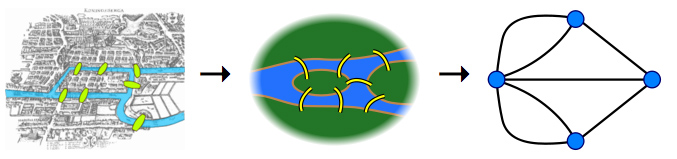
\includegraphics[width=0.9\textwidth]{Figures/bridges.jpg} \\
\smallskip
\small{\textit{Abstracción del problema de los Puentes de Königsberg: desde el mapa original hasta su representación como grafo.}} \
\href{https://en.wikipedia.org/wiki/File:Konigsberg_bridges.png}{\scriptsize{Imagen: Bogdan Giuşcă.}}
\end{center}

\subsection{Ejemplos de aplicaciones}
Los grafos no solo son una herramienta matemática elegante, sino también un lenguaje poderoso para representar sistemas complejos en el mundo real. A continuación, se presentan algunas aplicaciones concretas y ampliamente estudiadas del uso de grafos en distintas áreas del conocimiento y la tecnología \footnote{Barabási, A.-L. (2016). \href{http://networksciencebook.com/}{\textit{Network Science}}. Cambridge University Press.} 

\begin{itemize}
\item Modelar redes de comunicación: cada dispositivo es un nodo, y una conexión directa entre dos dispositivos (como un cable o enlace inalámbrico) se modela como una arista. Esto permite representar arquitecturas de red como topologías en estrella, anillo o malla, facilitando el análisis de eficiencia y tolerancia a fallos.

\item Representar relaciones sociales: personas como nodos y las amistades, interacciones o vínculos (como seguir a alguien en redes sociales) como aristas. Esta abstracción permite estudiar propiedades como centralidad, comunidades, y difusión de información.

\item Representar colaboraciones científicas: se construyen grafos donde cada nodo es un autor, y dos autores están conectados si han publicado juntos. Un ejemplo contemporáneo es el uso de bases de datos académicas para modelar la evolución de la colaboración interdisciplinaria.

\item Modelar el transporte: estaciones, paraderos o aeropuertos son nodos, y las rutas (como líneas de metro, vuelos o carreteras) son aristas. Esto permite optimizar rutas, estudiar congestión o conectividad.
\end{itemize}






\subsection{Clasificación de Grafos}

\subsection*{Tipos de grafos}
\begin{itemize}
\item \textbf{Grafo simple}: sin lazos ni aristas paralelas.
\item \textbf{Multigrafo}: permite aristas paralelas.
\item \textbf{Grafo con lazos}: permite aristas de un nodo a sí mismo.
\item \textbf{Grafos dirigidos}: las aristas tienen dirección.
\end{itemize}

\begin{center}
\begin{tabular}{lccc}
\toprule
\textbf{Nombre} & \textbf{Aristas} & \textbf{Aristas paralelas} & \textbf{Lazos} \\
\midrule
Grafo simple & No dirigidas & No & No \\
Multigrafo & No dirigidas & Sí & No \\
Grafo & No dirigidas & Sí & Sí \\
Grafo dirigido simple & Dirigidas & No & No \\
Multigrafo dirigido & Dirigidas & Sí & No \\
Grafo dirigido & Dirigidas & Sí & Sí \\
\bottomrule
\end{tabular}
\end{center}

\subsection{Terminología}

\subsubsection*{Grafos no dirigidos}
\begin{itemize}
\item Dos nodos son \textbf{adyacentes} si comparten una arista.
\item Una arista es \textbf{incidente} a un nodo si el nodo es uno de sus extremos.
\item El \textbf{grado} de un nodo $v$, denotado $\deg(v)$, es el número de aristas incidentes (los lazos cuentan doble).
\item Un nodo es \textbf{aislado} si $\deg(v) = 0$.
\end{itemize}

\subsubsection*{Grafos dirigidos}
\begin{itemize}
\item En una arista $(u,v)$, $u$ es el \textbf{origen} y $v$ el \textbf{destino}.
\item \textbf{Grado de entrada}: $\deg^{-}(v)$ es el número de aristas que llegan a $v$.
\item \textbf{Grado de salida}: $\deg^{+}(v)$ es el número de aristas que salen de $v$.
\end{itemize}




\subsection{Ejemplos empíricos: Distribución de grado en redes reales}
Una propiedad estructural fundamental de un grafo es su \textbf{distribución de grado}, que indica cuántos nodos tienen $k$ conexiones para cada posible valor de $k$. Esta distribución revela la organización global de la red y es especialmente importante en grafos grandes como los que aparecen en contextos reales.

En la siguiente figura se observan distribuciones de grado para diferentes redes reales, muchas de las cuales exhiben comportamientos que siguen una ley de potencias:

\begin{center}
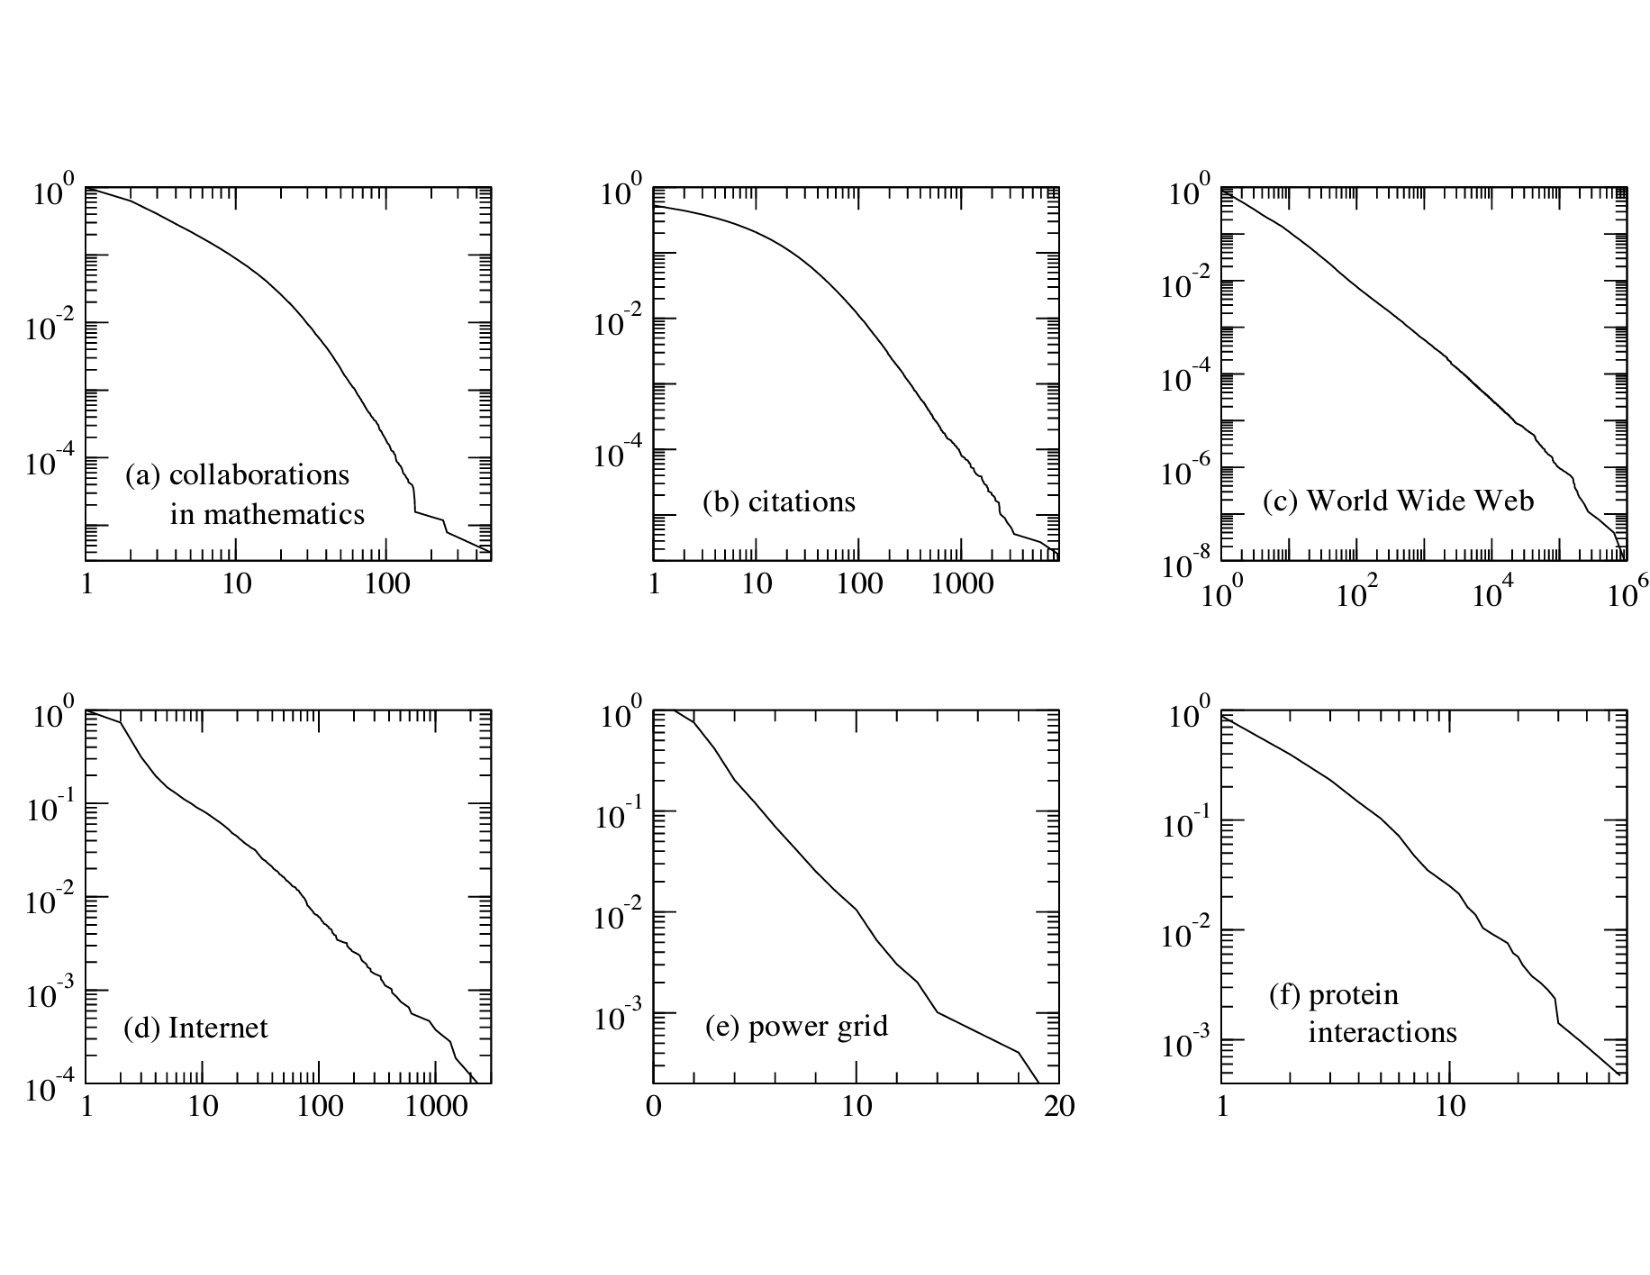
\includegraphics[width=0.8\textwidth]{Figures/power_law.pdf} \\
\small{\textit{Distribuciones de grado para diversas redes: colaboración matemática, citas, web, internet, red eléctrica y proteínas.}} 
\scriptsize{Fuente: Newman, M.E.J. (2003). \href{https://doi.org/10.1137/S003614450342480}{\textit{The Structure and Function of Complex Networks}}. \textit{SIAM Review}.}
\end{center}

\subsection*{Características comunes}

\begin{itemize}
\item En redes como la web, el internet o las redes sociales, la mayoría de los nodos tiene pocos enlaces, mientras que unos pocos tienen muchos (nodos \emph{hub}).
\item Este comportamiento es típico de una \textbf{distribución de grado sesgada} o de tipo \emph{escala libre}, en contraste con una red aleatoria.
\item En estos casos, la probabilidad de que un nodo tenga grado $k$ decrece como $P(k) \sim k^{-\gamma}$ para alguna constante $\gamma$.
\end{itemize}

Estas propiedades tienen consecuencias importantes: los hubs pueden facilitar la difusión rápida de información o infecciones, pero también pueden ser puntos vulnerables si fallan.




\section{Propiedades de los Grafos}
Una de las propiedad de los grafos no dirigidos es la relación entre el número total de aristas y los grados de los vértices. Esta relación se conoce comúnmente como el \emph{Teorema de los saludos}, ya que puede interpretarse en un contexto cotidiano: 
El número total de apretones de manos en una fiesta es igual a la suma de las manos estrechadas por cada persona, y por lo tanto, siempre es par. En consecuencia, el número de personas que da un número impar de apretones es par.

\begin{thmblock}{Teorema de los saludos}
Sea $G = (V, E)$ un grafo no dirigido. Entonces:
$$
\sum_{v \in V} \deg(v) = 2|E|
$$
En particular, \textbf{el número de nodos de grado impar es par}.
\end{thmblock}

\begin{proof}
El resultado es inmediato ya que cada arista $e \in E$ aporta dos unidades
a la suma $\sum_{v \in V} deg(v)$. (Puede probarse más
formalmente haciendo inducción sobre el número de aristas del grafo.)

\medskip

Para probar que el número de nodos de grado impar es par, consideremos la suma total $S = \sum_{v \in V} \deg(v)$ como una suma de enteros. Dado que $S$ es par (igual a $2|E|$), y que la suma de números impares sólo puede ser par si hay una cantidad par de sumandos impares, se deduce que debe haber un número par de vértices con grado impar.
\end{proof}

% \begin{exampleblock}{Ejemplo}
% Considere un grafo con $5$ vértices y $4$ aristas:
% \begin{itemize}
% \item $\deg(v_1) = 2$, $\deg(v_2) = 1$, $\deg(v_3) = 2$, $\deg(v_4) = 1$, $\deg(v_5) = 2$.
% \end{itemize}
% Entonces:

% Además, los vértices $v_2$ y $v_4$ tienen grado impar, y hay exactamente dos de ellos.
% \end{exampleblock}

\begin{thmblock}{Lema de grados para grafos dirigidos}
Sea $G=(V,E)$ un grafo dirigido. Entonces:

$$
\sum_{v \in V} \deg^{-}(v) = \sum_{v \in V} \deg^{+}(v) = |E|
$$
\end{thmblock}

\begin{proof}
Cada arista dirigida $(u,v) \in E$ tiene un nodo origen $u$ y un nodo destino $v$. Por definición, cada arista incrementa en uno el grado de salida de $u$ y el grado de entrada de $v$. Por lo tanto, al sumar los grados de salida y de entrada sobre todos los vértices, cada arista contribuye una única vez a cada suma:
$\sum_{v \in V} \deg^{-}(v) = |E|, \quad \sum_{v \in V} \deg^{+}(v) = |E|.$
\end{proof}

% \begin{exampleblock}{Ejemplo}
% Sea $G$ un grafo dirigido con tres aristas:
% $E = \{(v_1, v_2), (v_2, v_3), (v_3, v_1)\}.$
% Entonces:
% \begin{itemize}
% \item $\deg^{+}(v_1) = 1\$, \$\deg^{-}(v_1) = 1$
% \item $\deg^{+}(v_2) = 1\$, \$\deg^{-}(v_2) = 1$
% \item $\deg^{+}(v_3) = 1\$, \$\deg^{-}(v_3) = 1$
% \end{itemize}
% Y:
% $\sum_{v \in V} \deg^{+}(v) = \sum_{v \in V} \deg^{-}(v) = 3 = |E|.$
% \end{exampleblock}





\subsection{Ejemplos Clásicos de Grafos}

\begin{itemize}

\item \textbf{Cliques} ($K_n$): Todos los nodos están conectados entre sí.

\begin{center}
\begin{tikzpicture}[scale=1, every node/.style={circle, draw, fill=white, minimum size=0.6cm}]
  \foreach \k in {1,...,4} {
    \node (v\k) at ({90+90*(\k-1)}:1.5) {\k};
  }
  \foreach \k in {1,...,4} {
    \foreach \l in {1,...,4} {
      \ifnum\k<\l
        \draw (v\k) -- (v\l);
      \fi
    }
  }
\end{tikzpicture}
\end{center}

\item \textbf{Ciclos} ($C_n$): Un ciclo de $n \geq 3$ vértices $v_1,v_2,\dots,v_n$ es aquel grafo simple que contiene las aristas
$\{(v_1,v_2),(v_2,v_3),\dots,(v_{n-1},v_n),(v_n,v_1)\}$. Usamos $C_n$ para denotar al ciclo de $n$ vértices.

\begin{center}
\begin{tikzpicture}[scale=1, every node/.style={circle, draw, fill=white, minimum size=0.6cm}]
  \foreach \k in {1,...,6} {
    \node (v\k) at ({60*(\k-1)}:1.5) {\k};
  }
\foreach \i in {1,...,6} {
  \pgfmathtruncatemacro{\j}{mod(\i,6)+1}
  \draw (v\i) -- (v\j);
}
\end{tikzpicture}
\end{center}

\item \textbf{Grafos bipartitos}: Un grafo $G=(V,E)$ es bipartito sii $V$ puede ser particionado en dos conjuntos $V_1$ y $V_2$ tal que cada arco del grafo conecta un
nodo de $V_1$ con uno de $V_2$, y no hay arcos dentro de un mismo conjunto.conjuntos.

\begin{center}
\begin{tikzpicture}[scale=1.5, every node/.style={circle, draw, fill=white, minimum size=0.5cm}]
  \foreach \i in {1,...,3} {
    \node (a\i) at (0,2-\i) {$A_\i$};
    \node (b\i) at (2,2-\i) {$B_\i$};
    \draw (a\i) -- (b\i);
  }
  \draw (a1) -- (b2);
  \draw (a2) -- (b1);
  \draw (a3) -- (b2);
\end{tikzpicture}
\end{center}


\item \textbf{Grafos bipartitos completos} ($K_{m,n}$): Un grafo bipartito se dice además \textbf{completo} si existe un arco entre
\emph{cada} par de nodos $(u,v)$ tal que $u \in V_1$ y $v \in V_2$. Usamos
$K_{|V_1|,|V_2|}$ para denotar a dicho grafo. 

\begin{center}
\begin{tikzpicture}[scale=1.5, every node/.style={circle, draw, fill=white, minimum size=0.6cm}]
  \foreach \k in {1,...,2} {
    \node (a\k) at (0,2-\k) {$A_\k$};
  }
  \foreach \l in {1,...,3} {
    \node (b\l) at (2,2.5-\l) {$B_\l$};
  }
  \foreach \k in {1,...,2} {
    \foreach \l in {1,...,3} {
      \draw (a\k) -- (b\l);
    }
  }
\end{tikzpicture}
\end{center}

\end{itemize}


\begin{thmblock}{Caracterización de grafos bipartitos}
Un grafo simple es bipartito si y solo si sus vértices pueden colorearse con dos colores de forma que ningún par de nodos adyacentes tenga el mismo color.
\end{thmblock}
\begin{proof}
($\Rightarrow$) Suponga que $G = (V, E)$ es bipartito y que la partición de $V$ está dada por $V_1$ y $V_2$. Pinte los vértices en $V_1$ de azul y los vértices en $V_2$ de rojo. Como en un grafo bipartito todas las aristas conectan vértices de conjuntos distintos, ningún par de vértices adyacentes estará pintado del mismo color.

\medskip

($\Leftarrow$) Suponga ahora que es posible pintar de rojo o azul cada vértice de $G$ de tal forma que si dos nodos son adyacentes, entonces reciben colores distintos. Defina $V_1$ como el conjunto de nodos coloreados de azul y $V_2$ como el conjunto de nodos coloreados de rojo. Entonces $V = V_1 \cup V_2$ y toda arista conecta un nodo de $V_1$ con uno de $V_2$, lo que demuestra que $G$ es bipartito.
\end{proof}



\subsection{Ejercicios Propuestos}
\begin{enumerate}
\item Use el teorema anterior para determinar si los siguientes grafos son
bipartitos:
\begin{center}
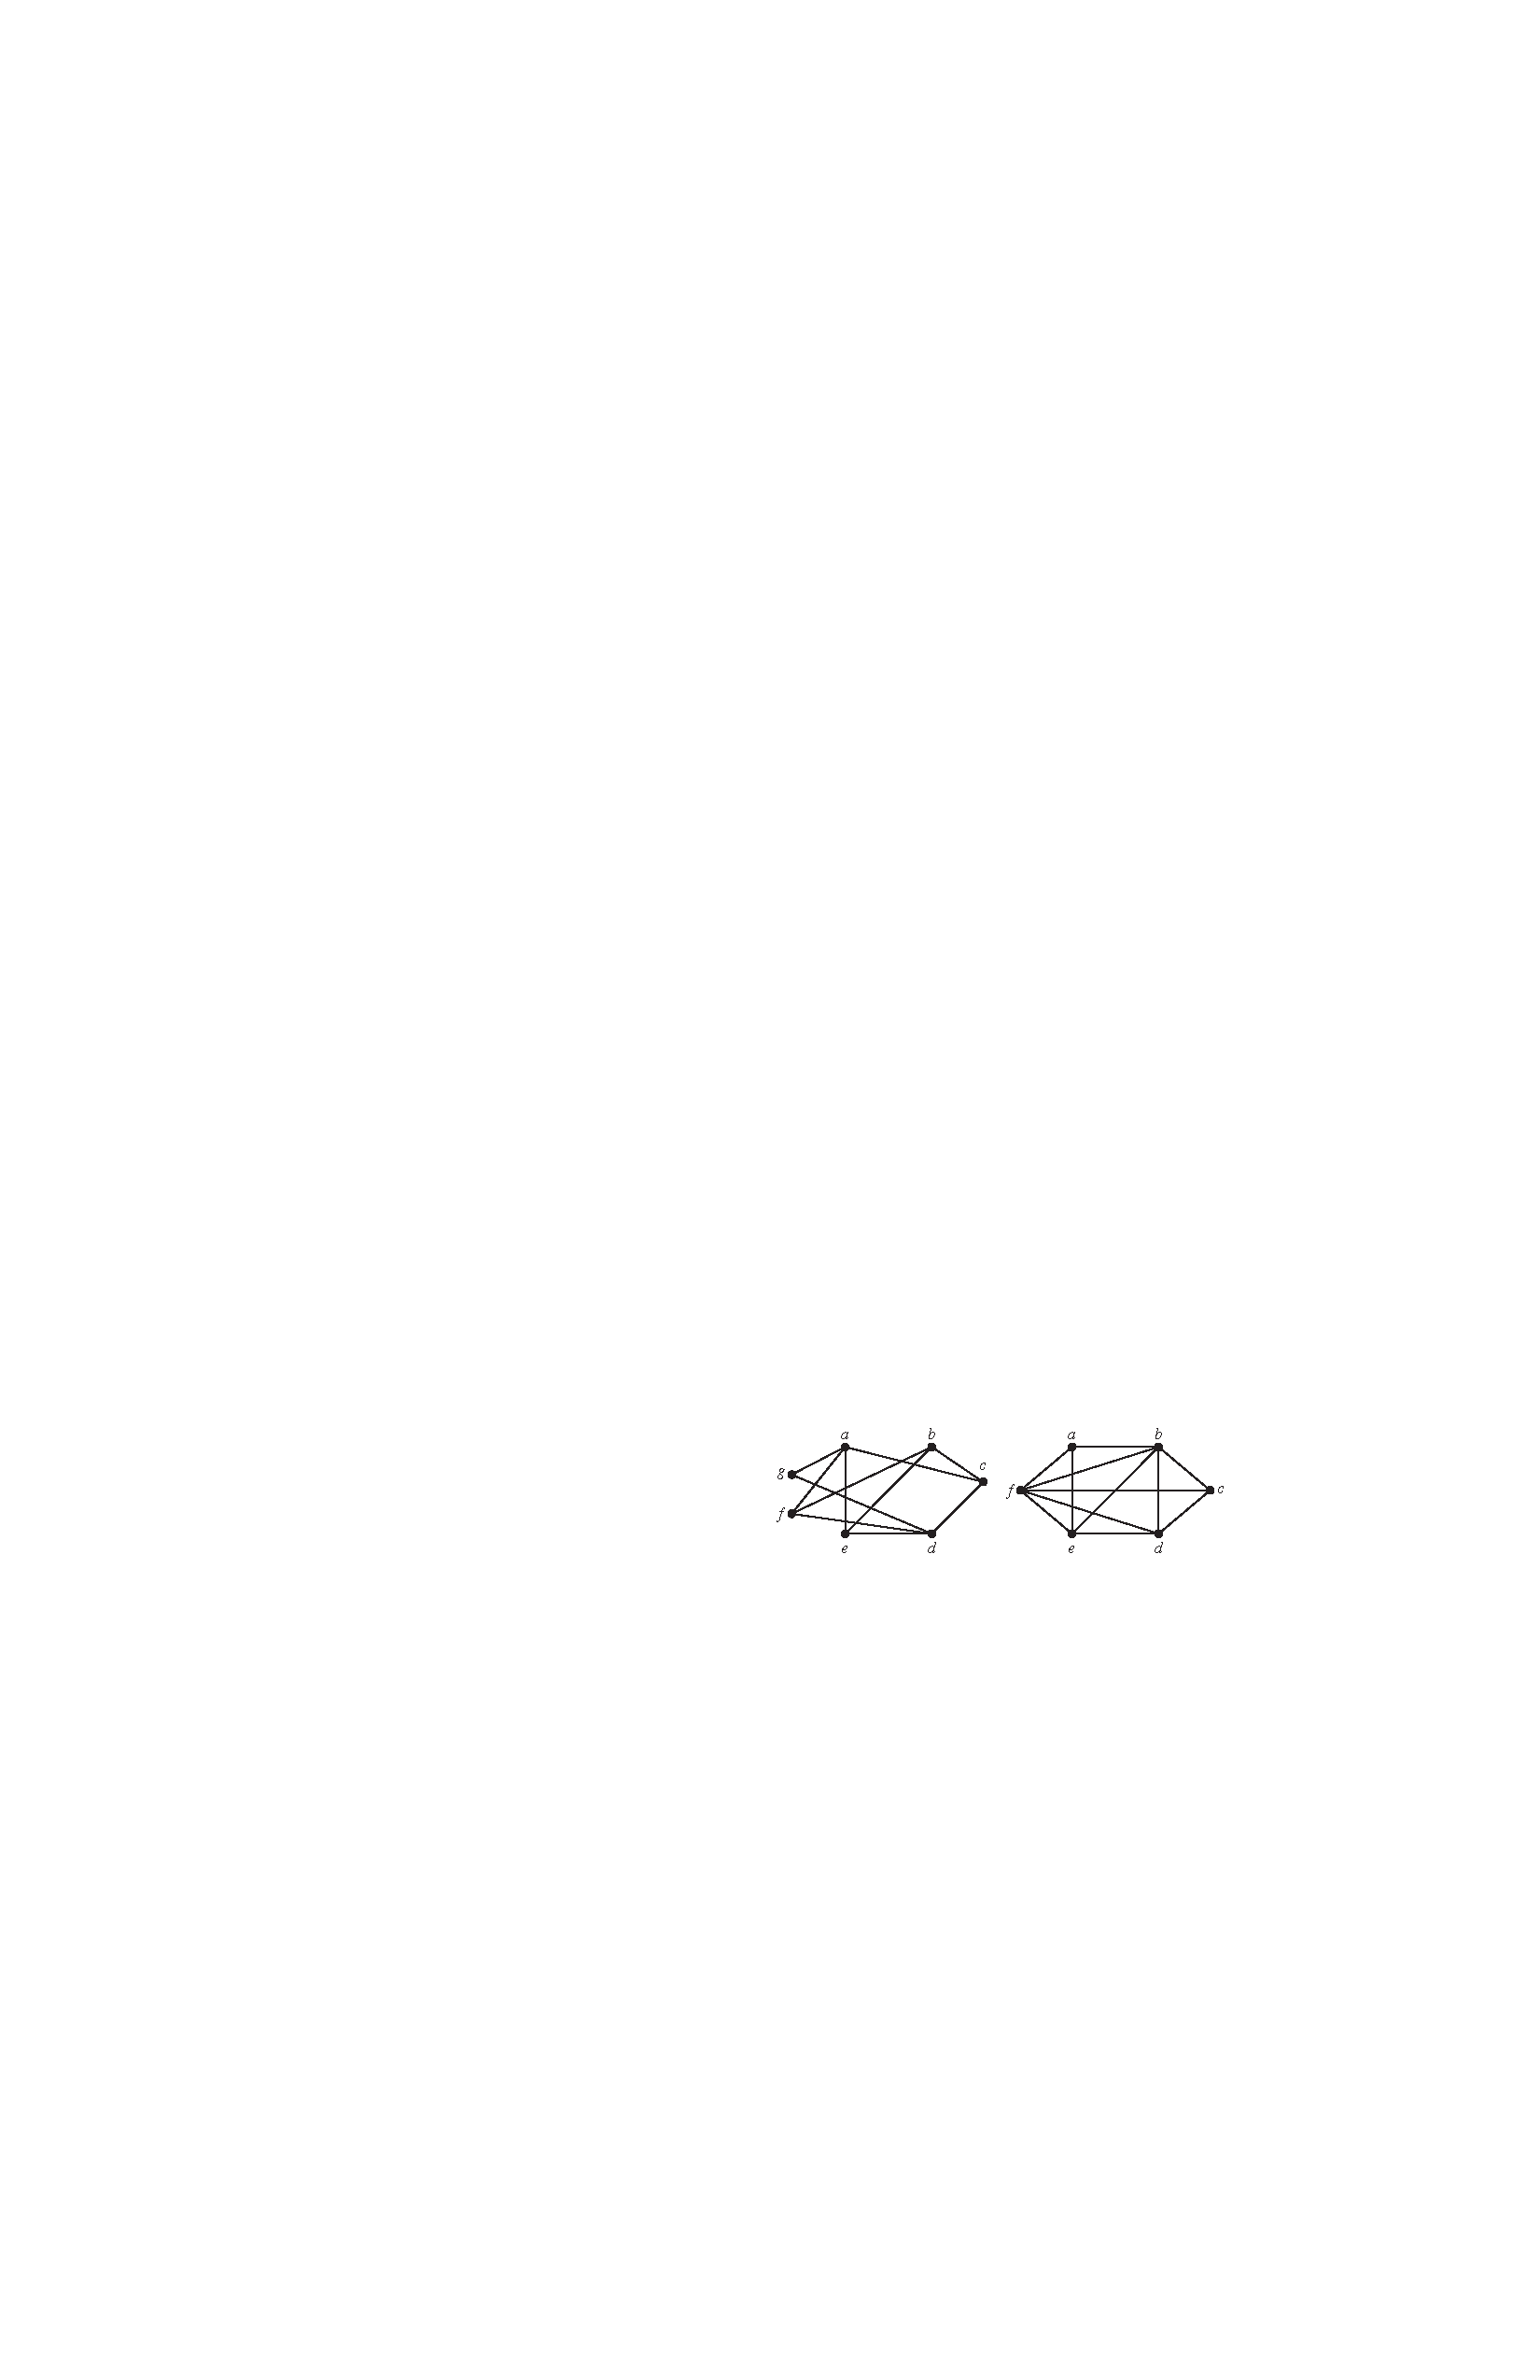
\includegraphics[width=0.7\textwidth]{Figures/ExerciseBipartite.pdf}
\end{center}
\item Demuestre que el ciclo $C_n$ es bipartito si y solo si $n$ es par.
\item Sea $G = (V,E)$ un grafo simple. Demuestre que $$ \min\,\{deg(v) \mid v \in V\} ~\leq~ \frac{2 \, |E|}{|V|} ~\leq~\max\, \{deg(v) \mid v \in V\}$$
\item  Sea $G = (V,E)$ un grafo bipartito simple. Demuestre que 
$|E| \leq |V|^2 / 4$. 
\end{enumerate}










% \title{Apunte de Matemáticas Discretas CC3101:\\ 
% Representación, subgrafos, isomorfismos y conectividad de grafos  Clase 18}
% % \title{Ejercicios Lógica e Inducción}
% \author{Andrés Abeliuk}
% \date{}
% \maketitle


\section{Representación de grafos}

Una vez que comprendemos la noción abstracta de grafo, surge una pregunta natural: ¿cómo podemos representar un grafo en un computador de manera que sea útil para analizarlo y procesarlo? 
Existen varias formas de representar un grafo, y la elección depende del tipo de operaciones que queremos realizar sobre él.

La representación elegida puede afectar considerablemente la eficiencia de los algoritmos. Por ejemplo, encontrar los vecinos de un nodo es muy eficiente en una lista de adyacencia, pero verificar si dos nodos están conectados es inmediato en una matriz de adyacencia. 


Consideremos el siguiente grafo simple, no dirigido, con cuatro v\'ertices:
\begin{figure}[h]
\centering
\begin{tikzpicture}[scale=1, every node/.style={circle, draw}]
  \node (a) at (0,1.5) {a};
  \node (b) at (-1.5,0) {b};
  \node (c) at (1.5,0) {c};
  \node (d) at (0,-1.5) {d};
  \draw (a) -- (b);
  \draw (a) -- (c);
  \draw (b) -- (d);
  \draw (c) -- (d);
  \draw (c) -- (b);
\end{tikzpicture}
\caption{Grafo base utilizado en las representaciones}
\label{fig:grafo-representaciones}
\end{figure}

Este grafo tiene:
\begin{itemize}
  \item V\'ertices: $V = \{a, b, c, d\}$
  \item Aristas: $E = \{(a,b), (a,c), (b,d), (c,d), (b,c)\}$
\end{itemize}
A continuaci\'on presentamos tres formas comunes para representar un grafo.

\subsection{Listas de adyacencia}

Una de las representaciones más comunes es la de \textbf{listas de adyacencia}, donde para cada vértice se mantiene una lista de sus vértices adyacentes.

\begin{definitionblock}{Lista de adyacencia}
Dado un grafo \( G = (V, E) \), una lista de adyacencia asocia a cada vértice \( v \in V \) un conjunto o lista de vértices adyacentes a \( v \), es decir, aquellos vértices \( u \in V \) tales que \( (v, u) \in E \).
\end{definitionblock}

\begin{exampleblock}{Ejemplo: Lista de adyacencia}
Lista de adyacencia correspondiente al grafo de la Figura~\ref{fig:grafo-representaciones}:
\begin{center}
\begin{tabular}{l|l}
V\'ertice & Adyacentes \\
\hline
a & b, c \\
b & a, c, d \\
c & a, b, d \\
d & b, c \\
\end{tabular}
\end{center}
\end{exampleblock}

Esta representación es eficiente en espacio cuando el grafo es \emph{disperso} (pocas aristas en relación al número de vértices).

\subsection{Matriz de adyacencia}

Otra forma clásica es la \textbf{matriz de adyacencia}, una matriz cuadrada de tamaño \( n \times n \), donde \( n = |V| \), que indica si existe una arista entre dos vértices.

\begin{definitionblock}{Matriz de adyacencia}
Sea \( G = (V, E) \) con \( V = \{v_1, v_2, \ldots, v_n\} \). La matriz de adyacencia \( A = [a_{ij}] \) se define como:
\[
a_{ij} =
\begin{cases}
1 & \text{si } (v_i, v_j) \in E \\
0 & \text{si } (v_i, v_j) \notin E
\end{cases}
\]
\end{definitionblock}

\begin{exampleblock}{Ejemplo: Matriz de adyacencia}
Matriz de adyacencia del grafo de la Figura~\ref{fig:grafo-representaciones}, en el orden \( a, b, c, d \):
\[
A = \begin{bmatrix}
0 & 1 & 1 & 0 \\
1 & 0 & 1 & 1 \\
1 & 1 & 0 & 1 \\
0 & 1 & 1 & 0
\end{bmatrix}
\]
\end{exampleblock}

Una propiedad interesante es que la matriz depende del orden de los vértices. Por tanto, un mismo grafo puede tener \( n! \) matrices distintas asociadas.

\subsection{Matriz de incidencia}

La tercera representación que estudiaremos es la \textbf{matriz de incidencia}, que vincula vértices con aristas.

\begin{definitionblock}{Matriz de incidencia}
Sea \( G = (V, E) \) con \( V = \{v_1, \ldots, v_n\} \) y \( E = \{e_1, \ldots, e_m\} \). La matriz de incidencia \( B = [b_{ij}] \) es una matriz \( n \times m \) donde:
\[
b_{ij} =
\begin{cases}
1 & \text{si el vértice } v_i \text{ es incidente en la arista } e_j \\
0 & \text{si no}
\end{cases}
\]
\end{definitionblock}

\begin{exampleblock}{Ejemplo: Matriz de incidencia}
Matriz de incidencia correspondiente al grafo de la Figura~\ref{fig:grafo-representaciones}, ordenando las aristas como: \( e_1 = (a,b), e_2 = (a,c), e_3 = (b,d), e_4 = (c,d), e_5 = (b,c) \):
\[
B = \begin{bmatrix}
1 & 1 & 0 & 0 & 0 \\
1 & 0 & 1 & 0 & 1 \\
0 & 1 & 0 & 1 & 1 \\
0 & 0 & 1 & 1 & 0
\end{bmatrix}
\]
\end{exampleblock}

Esta representación se utiliza frecuentemente en teoría de flujo y optimización lineal sobre redes.

\subsection*{Resumen y comparación}

\begin{center}
\resizebox{\textwidth}{!}{%
\begin{tabular}{l|c|c|c}
\textbf{Representaci\'on} & \textbf{Espacio} & \textbf{\'Eficiente para grafos densos?} & \textbf{\'Eficiente para grafos dispersos?} \\
\hline
Lista de adyacencia & \( O(n + m) \) & No & \textbf{S\'i} \\
Matriz de adyacencia & \( O(n^2) \) & \textbf{S\'i} & No \\
Matriz de incidencia & \( O(n \cdot m) \) & Intermedia & Intermedia \\
\end{tabular}
}
\end{center}

% \begin{quote}
% \textit{Curiosidad hist\'orica:} Las primeras matrices de adyacencia fueron utilizadas por el matem\'atico h\'ungaro D\'enes K\H{o}nig en su tratado pionero sobre teor\'ia de grafos en 1936.
% \end{quote}



\section{Subgrafos e Isomorfismo}

\subsection{Subgrafos}

En muchos casos, no es necesario considerar la totalidad de un grafo para resolver un problema. Basta con trabajar con una parte o ``fragmento'' de este.

\begin{definitionblock}{Subgrafo}
Sea $G = (V, E)$ un grafo. Un \textbf{subgrafo} de $G$ es un grafo $G' = (V', E')$ tal que $V' \subseteq V$ y $E' \subseteq E$. Decimos que el subgrafo es \textbf{propio} si $G' \neq G$.
\end{definitionblock}

\begin{exampleblock}{Ejemplo:}
En la Figura se muestra un grafo y un subgrafo resaltado en azul a su derecha.

\centering

\begin{tikzpicture}[scale=0.7, every node/.style={circle, draw, inner sep=2pt, font=\small}]

  % Grafo original
  \node (a) at (0,1.5) {a};
  \node (b) at (-1.5,0) {b};
  \node (c) at (1.5,0) {c};
  \node (d) at (0,-1.5) {d};
  \draw (a) -- (b);
  \draw (a) -- (c);
  \draw (c) -- (d);
  \draw (b) -- (d);

  % Subgrafo
  \node (a2) at (4,1.5) {a};
  \node (c2) at (5.5,0) {c};
  \node (d2) at (4,-1.5) {d};
  \draw[blue, very thick] (a2) -- (c2);
  \draw[blue, very thick] (c2) -- (d2);
\end{tikzpicture}
\end{exampleblock}

\subsection{Isomorfismo de grafos}

A veces dos grafos tienen distinta \emph{apariencia}, pero representan esencialmente la misma estructura. En tales casos decimos que los grafos son \textbf{isomorfos}.

\begin{definitionblock}{Isomorfismo}
Sean $G = (V,E)$ y $G' = (V',E')$ dos grafos simples. Decimos que $G$ y $G'$ son \textbf{isomorfos} si existe una biyecci\'on $f \colon V \to V'$ tal que para todo par de v\'ertices $v_1,v_2 \in V$, se cumple:
\[
(v_1,v_2) \in E \quad \text{si y s\'olo si} \quad \bigl(f(v_1),f(v_2)\bigr) \in E'
\]
A la funci\'on $f$ se le llama un \textbf{isomorfismo} entre $G$ y $G'$.
\end{definitionblock}

\begin{exampleblock}{Ejemplo:}
\begin{minipage}{0.45\textwidth}
A continuaci\'on se muestran dos grafos que, aunque visualmente diferentes, son isomorfos.
\end{minipage}%%
\hfill
\begin{minipage}{0.4\textwidth}
\centering
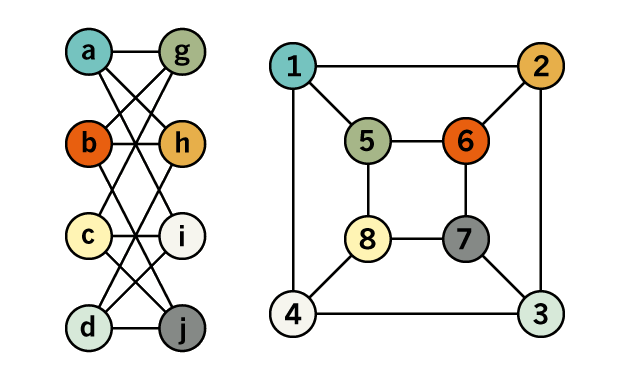
\includegraphics[width=\textwidth]{Figures/Isomorphism.png}
\end{minipage}
\end{exampleblock}


\begin{quote}
\textbf{Pregunta:} \textit{\'Cu\'antas posibles correspondencias (biyecciones) existen entre dos grafos simples con $n$ nodos?}
\end{quote}


\subsection{Demostrando isomorfismo y no isomorfismo}


Demostrar que dos grafos son isomorfos implica encontrar una biyecci\'on entre sus v\'ertices que preserve las adyacencias. Aunque conceptualmente directo, este problema es \textbf{computacionalmente costoso}. Los mejores algoritmos actuales para grafos generales tienen una complejidad \textbf{exponencial} en el n\'umero de v\'ertices. Por ello, es un problema central en el \textit{Graph Isomorphism Problem}, uno de los pocos problemas importantes cuya complejidad a\'{u}n no se conoce con certeza. 

La dificultad inherente en el problema de grafos isomorfos lo hacen un entretenido y desafiante puzzle:
\url{https://aabeliuk.github.io/graph-isomorphism-game/}


\subsubsection{Demostrando que dos grafos no son isomorfos}



\begin{exampleblock}{Ejemplo}
\textit{¿Són los siguientes grafos isomorfos?}
\begin{center}
\begin{tikzpicture}[scale=1.1, every node/.style={circle, draw, minimum size=6mm, font=\small}]
  % Grafo G
  \node (g1) at (0,1) {1};
  \node (g2) at (-1,0) {2};
  \node (g3) at (1,0) {3};
  \node (g4) at (0,-1) {4};
  \node (g5) at (0,0) {5};
  \draw (g1) -- (g2);
  \draw (g1) -- (g3);
  \draw (g2) -- (g4);
  \draw (g3) -- (g4);
  \draw (g5) -- (g2);
  \draw (g5) -- (g3);

  % Grafo H
  \node (h1) at (4,1) {a};
  \node (h2) at (3,0.3) {b};
  \node (h3) at (5,0.3) {c};
  \node (h4) at (3.5,-0.8) {d};
  \node (h5) at (4.5,-0.8) {e};
  \draw (h1) -- (h2);
  \draw (h1) -- (h3);
  \draw (h1) -- (h4);
  \draw (h1) -- (h5);
  \draw (h2) -- (h4);
  \draw (h3) -- (h5);
\end{tikzpicture}
\end{center}

\medskip

\textbf{Respuesta:} No, porque uno de los grafos  tiene un v\'ertice de grado 4 (el v\'ertice $a$), mientras que el otro grafo no tiene ning\'un v\'ertice con ese grado.
\end{exampleblock}



\medskip

Para demostrar que dos grafos \textbf{no} son isomorfos, basta encontrar una \textbf{propiedad invariante} bajo isomorfismos que difiera entre ambos. Algunas propiedades invariantes comunes son:

\begin{itemize}
  \item N\'umero de v\'ertices y aristas.
  \item Grado de los v\'ertices.
  \item Existencia de ciclos de ciertas longitudes.
  \item Distribuci\'on de componentes conexas.
\end{itemize}

Estas invariantes permiten descartar el isomorfismo sin necesidad de revisar todas las permutaciones posibles.


\subsubsection{Clases de isomorfismo}

\begin{thmblock}{Isomorfismo es clase de equivalencia}
Demostrar que la relaci\'on de isomorf\'ia entre grafos define una relaci\'on de equivalencia en la colecci\'on de todos los grafos.

\textbf{Hint:} Demostrar que la relaci\'on es reflexiva, sim\'etrica y transitiva.
\end{thmblock}



\medskip

Dado que el isomorfismo de grafos es una relaci\'on de equivalencia, divide el conjunto de todos los grafos en \textbf{clases de equivalencia}.
No importa cu\'al de los grafos isom\'orficos de una clase de equivalencia se escoja: todos comparten la misma estructura esencial.

\textbf{Aplicaciones:} Esta idea de clasificar grafos en clases de isomorfismo tiene múltiples aplicaciones en distintas áreas. Permite representar moléculas como grafos y detectar compuestos equivalentes. En \textbf{bases de datos de grafos}, se utiliza para identificar duplicados estructurales, incluso si los nombres de los nodos difieren. En \textbf{reconocimiento de patrones}, ayuda a comparar estructuras como árboles sintácticos o redes neuronales. Finalmente, en \textbf{algoritmos}, permite optimizar procedimientos al operar sobre representaciones canónicas de clases de grafos equivalentes.

\subsubsection{Ejercicios sobre isomorfismo}

El \textbf{complemento} de un grafo simple $G = (V,E)$ es el grafo $\overline G = (V,\overline E)$, tal que
\[(v_1,v_2) \in \overline{E} \Leftrightarrow (v_1,v_2) \not \in E.\]
Un grafo simple es \textbf{auto-complementario} si $G$ es isomorfo a $\bar G$.

\begin{itemize}
  \item \textbf{Ejercicio:} Demuestre que el siguiente grafo es auto-complementario.
  \begin{center}
  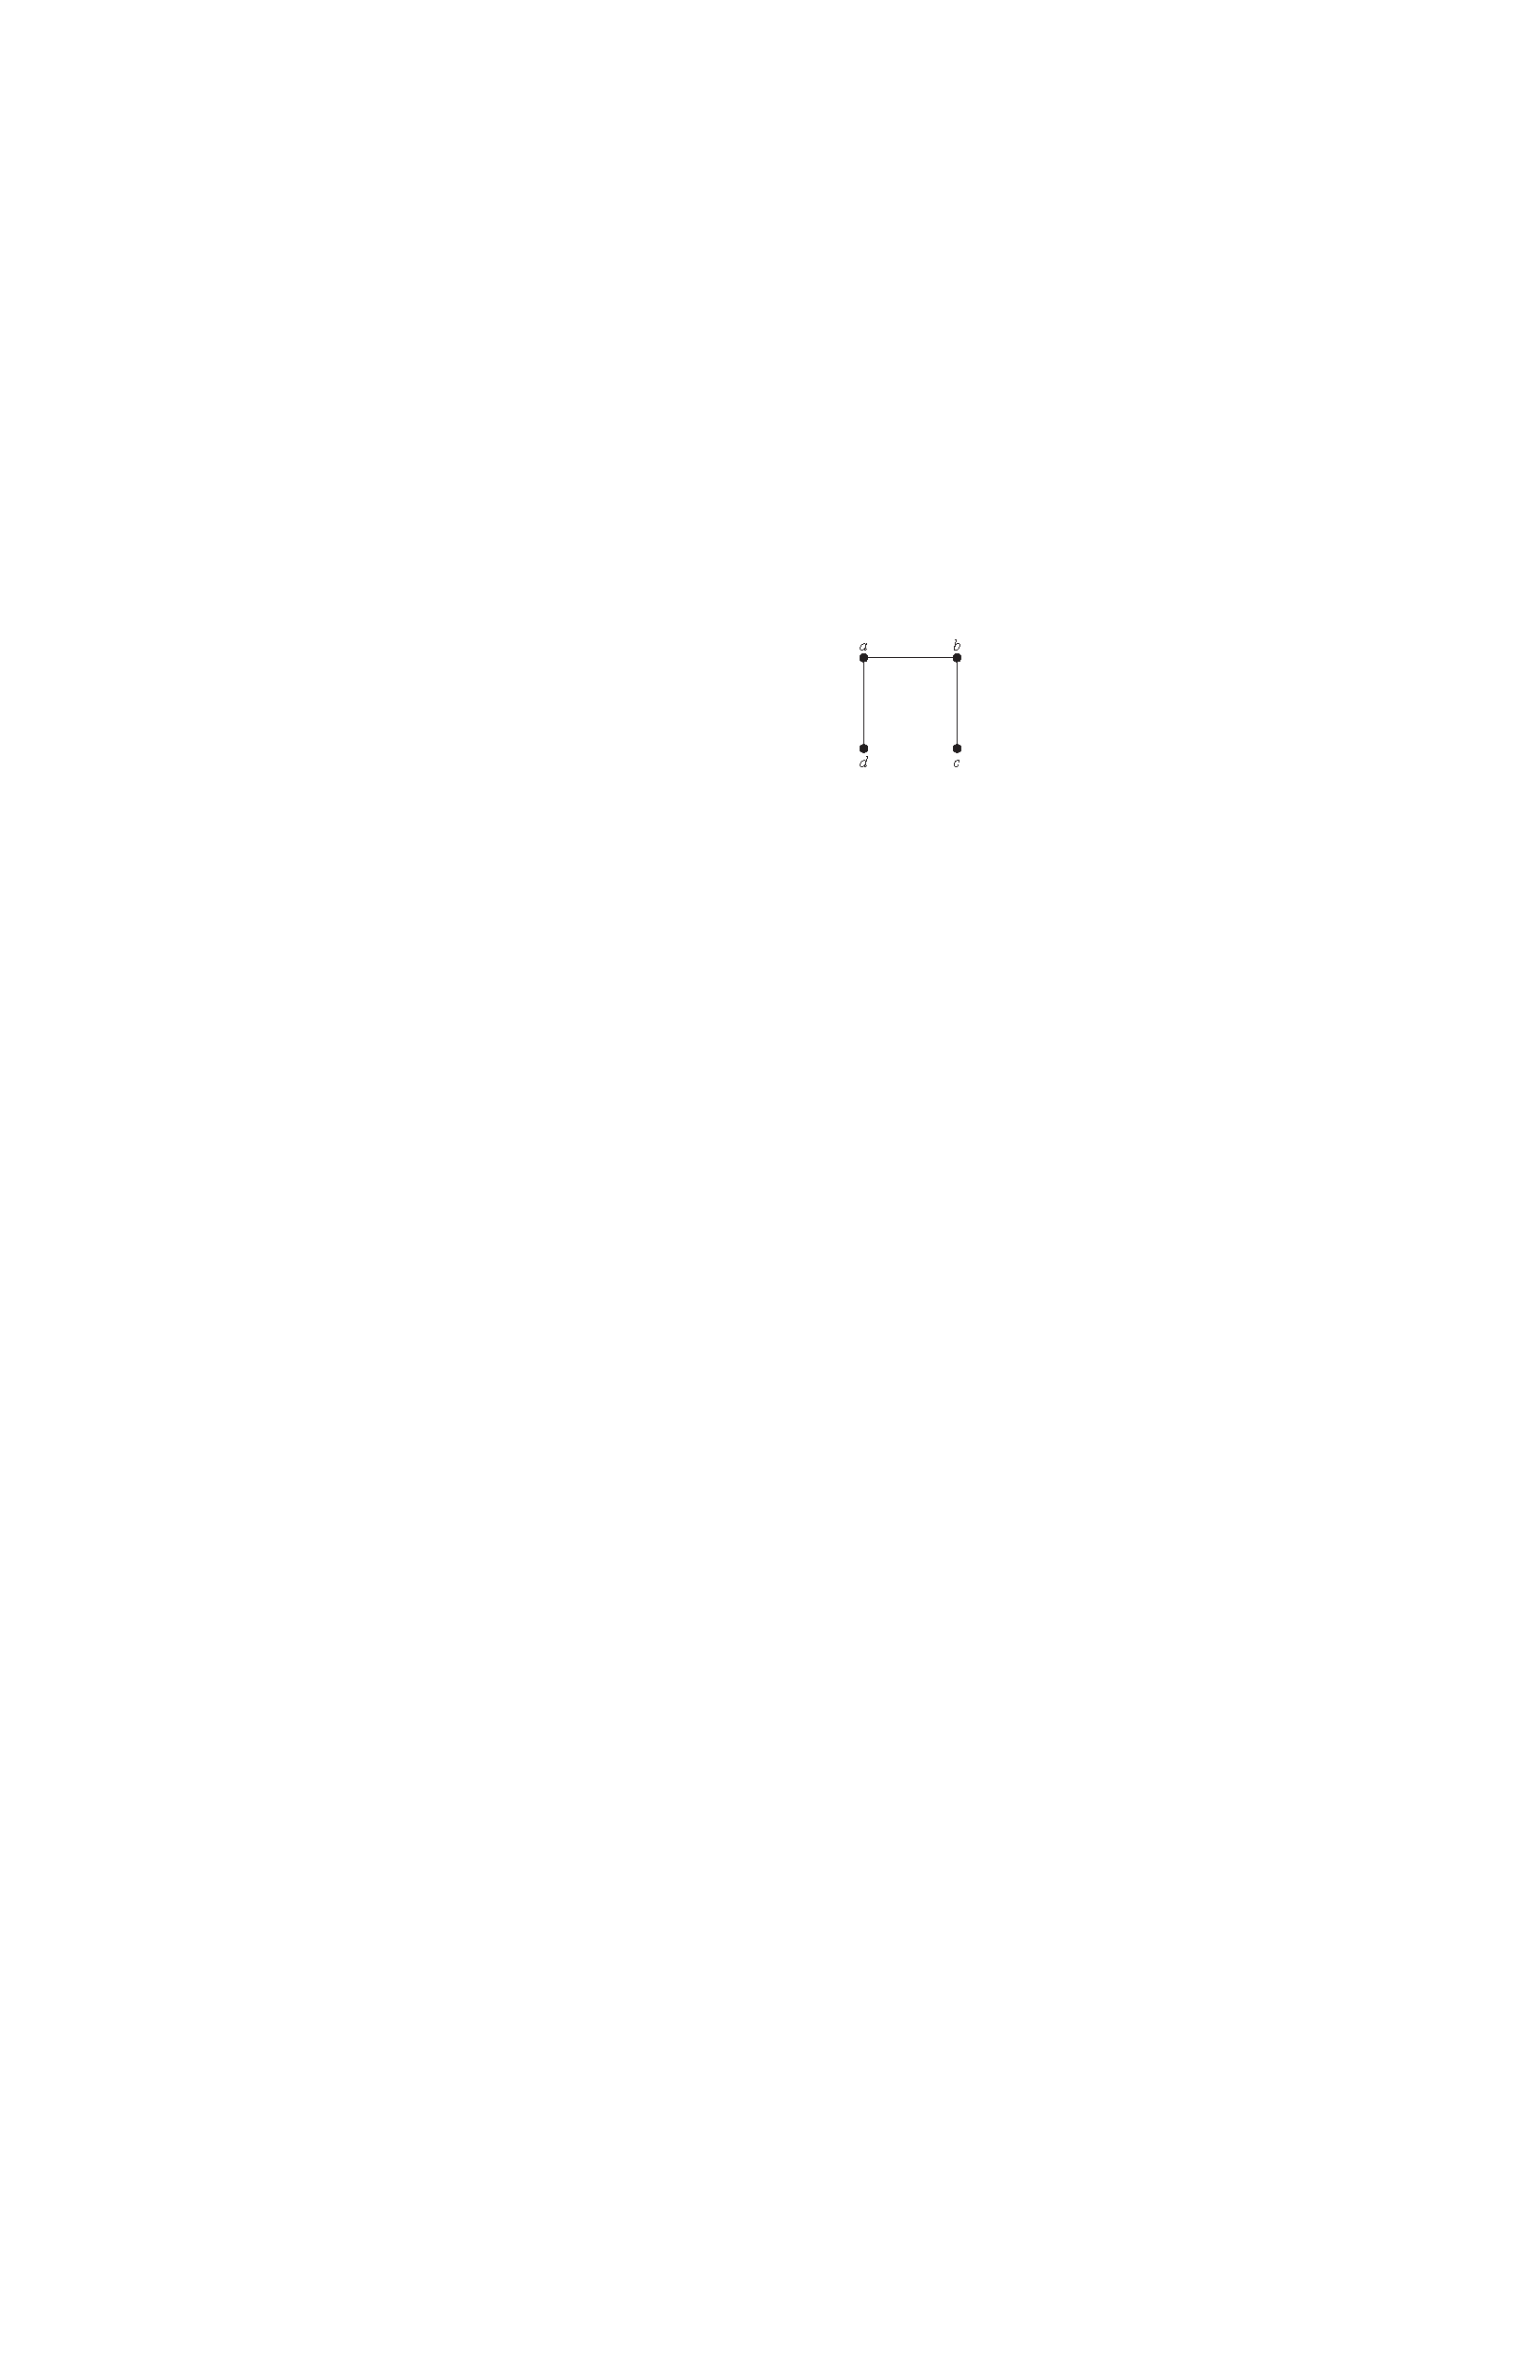
\includegraphics[width=0.15\textwidth]{Figures/SelfComplementary.pdf}
  \end{center}

  \item \textbf{Ejercicio:} Encuentre un grafo auto-complementario con 5 v\'ertices.

  % \item \textbf{Ejercicio:} \textquestiondown Para cu\'ales enteros $n$, el ciclo $C_n$ es auto-complementario?

  \item \textbf{Ejercicio:} Demuestre que si $G$ es un grafo auto-complementario simple con $n$ v\'ertices, entonces $n \equiv 0$ o $n \equiv 1$ m\'odulo 4.

 \item \textbf{Ejercicio:} ¿Cuántos grafos no isomorfos de 4 vértices existen? Dibújelos todos y justifique por qué no hay más.

\end{itemize}



\section{Caminos en grafos}

\subsection{Navegando grafos}

Muchos problemas pueden modelarse y resolverse \textbf{navegando grafos}. La noción de \textbf{camino} nos permite formalizar preguntas relacionadas con conectividad, eficiencia de recorrido y planificación de rutas.

\begin{itemize}
  \item \textbf{Ejemplo:} ¿Es posible mandar un mensaje entre dos computadoras usando las conexiones intermedias? Este problema puede resolverse explorando los caminos en una red.
  \item \textbf{Ejemplo:} ¿Cuál es la manera más rápida de salir de una granja, pasar por todos los establecimientos, y regresar al punto de partida? Esta es una instancia clásica del \textit{Problema del Viajante} (TSP).
\end{itemize}



\subsection{Definición de camino}

\begin{definitionblock}{Camino}
Sea $G = (V,E)$ un grafo no dirigido y sea $u,u' \in V$. Un \textbf{camino} (de largo $n$) entre $u$ y $u'$ es una secuencia de $n$ aristas $e_1, e_2, \ldots, e_n$ tal que existen nodos $v_0,v_1,v_2,\dots,v_n$ que satisfacen:
\begin{itemize}
  \item $v_0 = u$ y $v_n = u'$, y
  \item cada arista $e_i$ conecta $v_{i-1}$ y $v_i$, para $1 \leq i \leq n$
\end{itemize}
\end{definitionblock}

\begin{itemize}
  \item Si el camino no tiene aristas repetidas, se dice que es un \textbf{camino simple}.
  \item Si $u = u'$, entonces el camino se denomina \textbf{circuito} o \textbf{ciclo}.
\end{itemize}

\textbf{Notación:} Si el grafo no contiene aristas paralelas, podemos denotar un camino como la secuencia de vértices: $u,v_1,v_2,\ldots,v_{n-1},u'$.


\subsection{Conectividad de grafos no dirigidos}
En algunos grafos siempre es posible ir (i.e.~conectar mediante un camino) desde un vértice hasta cualquier otro. En otros no.

\begin{figure}[h!]
  \centering
  \begin{tikzpicture}[scale=1, every node/.style={circle, draw, minimum size=5mm, font=\small}]
    % Grafo conexo
    \node (a) at (0,1.5) {a};
    \node (b) at (-1,0.5) {b};
    \node (c) at (1,0.5) {c};
    \node (d) at (0,-0.5) {d};
    \node (e) at (2,1.5) {e};
    \draw (a) -- (b);
    \draw (a) -- (c);
    \draw (b) -- (d);
    \draw (c) -- (d);
    \draw (c) -- (e);

    % Separación
  
    % Grafo no conexo
    \node (f) at (5,1.5) {a};
    \node (g) at (6,0.5) {b};
    \node (h) at (4,0.5) {c};
    \draw (f) -- (g);
    \draw (f) -- (h);

    \node (i) at (4.5,-0.5) {d};
    \node (j) at (5.5,-0.5) {e};
    \draw (i) -- (j);
  \end{tikzpicture}
  \caption{Ejemplos de grafo conexo (izquierda) y no conexo (derecha)}
\end{figure}


\begin{definitionblock}{Conectividad}
Un grafo no dirigido se llama \textbf{conexo} sii existe un camino entre cada par de vértices distintos del grafo.
\end{definitionblock}

\begin{paragraph}{Propiedades e implicancias}
\leavevmode

Si existe un camino de $u$ a $v$ en un grafo $G = (V,E)$, entonces existe también un \textbf{camino simple} entre estos vértices. Esto es importante porque muchos algoritmos y teoremas operan sobre caminos simples, ya que descartan redundancias o ciclos intermedios.

Además, los caminos permiten definir \textbf{invariantes estructurales}, como la conectividad entre pares de vértices o la cantidad de componentes conexas. Estas invariantes pueden utilizarse para demostrar que dos grafos \textbf{no} son isomorfos, ya que todo isomorfismo debe preservar tales propiedades. Por ejemplo, si un grafo es conexo y otro no, no pueden ser isomorfos.
\end{paragraph}


\subsection{Componentes conexas}

Si un grafo es no conexo, entonces está formado por la unión disjunta de sus \textbf{componentes conexas}.

\begin{figure}[h]
  \centering
  \begin{tikzpicture}[every node/.style={circle, draw, fill=black, inner sep=1pt}, font=\small]
    % Componente H1
    \node (a) at (1,-1)  [label=below:$a$] {};
    \node (b) at (0.2,-0.1) [label=left:$b$] {};
    \node (c) at (1.8,-0.1)  [label=right:$c$] {};
    \draw (a) -- (b) -- (c) -- (a);
    \draw[rounded corners, blue] (-0.2, -1.4) rectangle (2.2, 0.3);
    \node[draw=none, fill=none, text=blue] at (1,0.55) {$H_1$};

    % Componente H2
    \node (d) at (2.7,0.9)  [label=above:$d$] {};
    \node (e) at (3.7,0.9)  [label=above:$e$] {};
    \draw (d) -- (e);
    \draw[rounded corners, blue] (2.5, 0.6) rectangle (3.9, 1.3);
    \node[draw=none, fill=none, text=blue] at (3.2,1.5) {$H_2$};

    % Componente H3
    \node (f) at (5,0.4)  [label=right:$f$] {};
    \node (g) at (5.8,-0.5) [label=right:$g$] {};
    \node (h) at (5,-1.4) [label=left:$h$] {};
    \draw (f) -- (g);
    \draw (g) -- (h);
    \draw[rounded corners, blue] (4.6, -1.7) rectangle (6.1, 0.7);
    \node[draw=none, fill=none, text=blue] at (5.4, 0.9) {$H_3$};
  \end{tikzpicture}
  \caption{Ejemplo de grafo no conexo con tres componentes conexas $H_1$, $H_2$ y $H_3$}
\end{figure}



\begin{definitionblock}{Componente conexa}
Sea $G$ un grafo no dirigido. Una \textbf{componente conexa} de $G$ es un subgrafo $G'$ de $G$ tal que:
\begin{itemize}
  \item $G'$ es conexo, y
  \item $G'$ no es un subgrafo propio de otro subgrafo conexo de $G$.
\end{itemize}
En otras palabras, una componente conexa de $G$ es un subgrafo conexo \textbf{maximal}.
\end{definitionblock}

\subsection{Conectividad de grafos dirigidos}

Hay dos variantes de la noción de conectividad sobre grafos dirigidos: una considerando la dirección de los arcos y otra no. Para esta última, necesitamos la noción de grafo no-dirigido \textbf{subyacente}.

\begin{definitionblock}{Grafo no-dirigido subyacente}
Dado un grafo dirigido $G = (V,E)$, el \textbf{grafo no-dirigido subyacente} $G'$ de $G$ se obtiene a partir de $G$, computando la clausura simétrica de su conjunto de aristas $E$.
\end{definitionblock}

\begin{figure}[h!]
  \centering
  \begin{tikzpicture}[every node/.style={circle, draw, minimum size=6mm, font=\small}]
    % Grafo no dirigido (izquierda)
    \node (a) at (0,1.5) {1};
    \node (b) at (-1,0) {2};
    \node (c) at (1,0) {3};
    \draw (a) -- (b);
    \draw (a) -- (c);
    \draw (b) -- (c);

    % Grafo dirigido (derecha)
    \node (d) at (4,1.5) {1};
    \node (e) at (3,0) {2};
    \node (f) at (5,0) {3};
    \draw[->] (d) -- (e);
    \draw[->] (d) -- (f);
    \draw[->] (e) -- (f);
    \draw[->] (f) to[bend left] (e);
  \end{tikzpicture}
  \caption{Ejemplo de grafo no dirigido (izquierda) y grafo dirigido (derecha) con arcos entre nodos}
\end{figure}

\subsubsection{Conectividad fuerte y débil en grafos dirigidos}

\begin{definitionblock}{Conectividad en grafos dirigidos}
\begin{itemize}
  \item Un grafo dirigido es \textbf{fuertemente conexo} si para todo par de vértices $v, v'$, existe un camino dirigido de $v$ a $v'$ y viceversa.
  \item Un grafo dirigido es \textbf{débilmente conexo} si su grafo no dirigido subyacente es conexo, es decir, si para todo par $v, v'$ existe un camino entre ellos ignorando las direcciones.
\end{itemize}
\end{definitionblock}

\begin{figure}[h]
  \centering
  \begin{tikzpicture}[>=latex, every node/.style={circle, draw, minimum size=6mm, font=\small}]
    % Weakly connected graph
    \node (w1) at (0,2) {1};
    \node (w2) at (-1,1) {2};
    \node (w3) at (-2,0) {3};
    \node (w4) at (0,0) {4};
    \draw[->] (w1) to[out=120,in=60,loop] (w1);
    \draw[->] (w1) -- (w2);
    \draw[->] (w2) -- (w3);
    \draw[->] (w2) -- (w4);

    \node[draw=none] at (-1, -0.8) {{\footnotesize \textbf{Débilmente conexo}}};

    % Strongly connected graph
    \node (s1) at (4,2) {1};
    \node (s2) at (3,0.5) {2};
    \node (s3) at (5,0.5) {3};
    \draw[->] (s1) to[out=120,in=60,loop] (s1);
    \draw[->] (s1) -- (s2);
    \draw[->] (s2) -- (s3);
    \draw[->] (s3) -- (s1);

    \node[draw=none] at (4,-0.8) {{\footnotesize \textbf{Fuertemente conexo}}};
  \end{tikzpicture}
  \vspace{-4em}
  \caption{Comparación entre grafo débilmente conexo (izquierda) y fuertemente conexo (derecha)}
\end{figure}



\subsubsection{Componentes fuertemente conexas}

\begin{definitionblock}{Componente fuertemente conexa}
Sea $G$ un grafo dirigido. Una \textbf{componente fuertemente conexa} de $G$ es un subgrafo dirigido $G'$ tal que:
\begin{itemize}
  \item $G'$ es fuertemente conexo, y
  \item $G'$ no es un subgrafo propio de otro subgrafo fuertemente conexo de $G$.
\end{itemize}
\end{definitionblock}



\subsection{Caminos e isomorfismo}

La existencia de ciertos caminos también puede usarse como \textbf{invariante} para distinguir grafos no isomorfos.

\begin{exampleblock}{Ejemplo}
Utilice un invariante de caminos para demostrar que los grafos de la Figura~\ref{figure:ex_iso} no son isomorfos.

\medskip

\textbf{Respuesta:} Aunque los grafos tienen la misma cantidad de nodos y aristas, así como los mismos grados, el grafo $H$ tiene un circuito simple de largo 3 ($v_1,v_2,v_6,v_1$), mientras que $G$ no posee ninguno. Esto muestra que no pueden ser isomorfos.
\end{exampleblock}

\begin{figure}[h]
  \centering
  \begin{tikzpicture}[scale=1, every node/.style={circle, draw, fill=black, inner sep=1.2pt}, font=\small]
    % Grafo G
    \node (u1) at (0,2) [label=above:$u_1$] {};
    \node (u2) at (1.2,1) [label=right:$u_2$] {};
    \node (u3) at (1.2,0) [label=right:$u_3$] {};
    \node (u4) at (0,-1) [label=below:$u_4$] {};
    \node (u5) at (-1.2,0) [label=left:$u_5$] {};
    \node (u6) at (-1.2,1) [label=left:$u_6$] {};

    \draw (u1) -- (u2) -- (u3) -- (u4) -- (u5) -- (u6) -- (u1);
    \draw (u6) -- (u3);
    \draw (u2) -- (u5);
    % \node[draw=none]  at (0,-1.6) {\textcolor{cyan}{$G$}};
    

    % Grafo H
    \begin{scope}[xshift=5cm]
      \node (v1) at (0,2) [label=above:$v_1$] {};
      \node (v2) at (1.2,1) [label=right:$v_2$] {};
      \node (v3) at (1.2,0) [label=right:$v_3$] {};
      \node (v4) at (0,-1) [label=below:$v_4$] {};
      \node (v5) at (-1.2,0) [label=left:$v_5$] {};
      \node (v6) at (-1.2,1) [label=left:$v_6$] {};

      \draw (v1) -- (v2) -- (v3) -- (v4) -- (v5) -- (v6) -- (v1);
      \draw (v6) -- (v2);
      \draw (v5) -- (v3);
      % \node at (0,-1.6) {\textcolor{cyan}{$H$}};
    \end{scope}
  \end{tikzpicture}
  \caption{Dos grafos $G$ y $H$}
  \label{figure:ex_iso}
\end{figure}




\subsection{Ejercicios}

\begin{itemize}
  \item \textbf{Ejercicio:} Demuestre que para todo grafo conexo simple, todo nodo de grado impar está unido mediante un camino a algún otro nodo de grado impar.

  \item \textbf{Ejercicio:} Demuestre que todo grafo conexo con $n$ vértices debe tener al menos $n-1$ aristas.

  \item \textbf{Ejercicio:} Demuestre que un grafo simple $G$ es bipartito si y sólo si no contiene circuitos de largo impar.
\end{itemize}

% \title{Apunte de Matemáticas Discretas CC3101:\\ 
% Caminos,  circuitos eulerianos y hamiltonianos  Clase 19}
% % \title{Ejercicios Lógica e Inducción}
% \author{Andrés Abeliuk}
% \date{}
% \maketitle


\section{Circuitos Eulerianos}

\subsection{El Problema de los Puentes de Königsberg}

En el siglo XVIII, en la ciudad prusiana de Königsberg, se planteó una pregunta curiosa sobre la posibilidad de recorrer la ciudad cruzando todos sus puentes exactamente una vez. La ciudad estaba dividida por el río Pregel en cuatro regiones conectadas por siete puentes.

\begin{center}
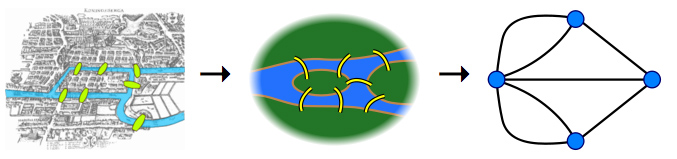
\includegraphics[width=0.9\textwidth]{Figures/bridges.jpg} \\
\smallskip
\small{\textit{Abstracción del problema de los Puentes de Königsberg: desde el mapa original hasta su representación como grafo.}} \
\href{https://en.wikipedia.org/wiki/File:Konigsberg_bridges.png}{\scriptsize{Imagen: Bogdan Giuşcă.}}
\end{center}

\begin{quote}
\textbf{Problema:} ¿Es posible comenzar en una región cualquiera, recorrer todos los puentes exactamente una vez, y volver al punto de partida?
\end{quote}

Este problema intrigó a los matemáticos de la época, y fue Leonhard Euler quien, en 1736, ofreció una solución formal, dando origen a la teoría de grafos.

\subsection{Modelado con Grafos}

Podemos modelar este problema mediante un \textbf{grafo}, donde cada región se representa con un vértice y cada puente con una arista que conecta dos vértices.

\begin{center}
\begin{tikzpicture}[scale=1, every node/.style={circle, draw}]
  \node (A) at (0,0) {A};
  \node (B) at (4,0) {B};
  \node (C) at (2,2) {C};
  \node (D) at (2,-1.5) {D};

  \draw (A) to[bend left=20] (C);
  \draw (A) to[bend right=20] (C);
  \draw (B) to[bend left=20] (C);
  \draw (B) to[bend right=20] (C);
  \draw (D) -- (C);
  \draw (A) -- (D);
  \draw (B) -- (D);
\end{tikzpicture}
\end{center}

El problema se convierte ahora en determinar si existe un \textbf{circuito euleriano} en este grafo.

\medskip

\begin{definitionblock}{Definición: Circuito Euleriano}
Sea $G$ un grafo. Un \emph{circuito euleriano} es un circuito simple que recorre cada arista de $G$ exactamente una vez.
\end{definitionblock}

\begin{exampleblock}{Ejemplo}
El siguiente grafo posee múltiples circuitos eulerianos:

\begin{center}
\begin{tikzpicture}[scale=1.3, every node/.style={circle, draw, fill=white, minimum size=6mm}]
  \node (A) at (-1,0) {A};
  \node (B) at (-1,-1) {B};
  \node (C) at (0,-1) {C};
  \node (F) at (1,-1) {F};
  \node (E) at (1,0) {E};
  \node (D) at (0,1) {D};

  \draw (A) -- (B);
  \draw (A) -- (C);
  \draw (A) -- (D);
  \draw (A) -- (E);
  \draw (B) -- (C);
  \draw (C) -- (F);
  \draw (C) -- (E);
  \draw (E) -- (F);
  \draw (D) -- (E);
\end{tikzpicture}
\end{center}

Algunos circuitos eulerianos posibles (empezando en $A$) son:
\[
ADEACEFCBA \quad \text{y} \quad AECABCFEDA
\]
\end{exampleblock}

\begin{thmblock}{Teorema Clásico de Euler}
Un multigrafo conexo tiene un circuito euleriano si y sólo si todos sus vértices tienen grado par.
\end{thmblock}

\subsection{Solución al problema de los puentes de Königsberg}

El problema de los puentes de Königsberg no tiene solución: el grafo que lo representa tiene cuatro vértices de grado impar, lo cual impide la existencia de un circuito euleriano. Este resultado marcó el inicio del estudio sistemático de grafos, un área fundamental en la matemática discreta y la informática.

\subsection{Demostración del Teorema de Euler}

\textbf{($\Rightarrow$)} Supongamos que $G$ tiene un circuito euleriano. Cada vez que el circuito pasa por un vértice, debe entrar y luego salir por aristas distintas, lo que contribuye con dos al grado de ese vértice. Como el circuito pasa por todas las aristas del grafo (por definición), y $G$ es conexo, todos los vértices deben tener grado par.

\medskip

\textbf{($\Leftarrow$)} Supongamos ahora que $G$ es conexo y que todos sus vértices tienen grado par. Construiremos un circuito euleriano de forma constructiva:

\begin{itemize}
  \item Elegimos un vértice cualquiera \( v_0 \) y un arco \( (v_0, v_1) \) incidente.
  \item Continuamos extendiendo un camino \( v_0, v_1, v_2, \dots, v_n \) de forma que no repita aristas y se detenga sólo cuando no sea posible continuar.
\end{itemize}

\begin{thmblock}{Proposición}
En el procedimiento anterior, necesariamente se cumple \( v_0 = v_n \), es decir, se obtiene un circuito.
\end{thmblock}

\begin{proof}
Supongamos lo contrario: que \( v_0 \neq v_n \). Entonces el camino termina en un vértice \( v_n \) con grado impar (ya que entró una sola vez). Pero esto contradice la hipótesis de que todos los vértices tienen grado par. Por lo tanto, el circuito debe cerrar.
\end{proof}

Por lo tanto tenemos un circuito simple 
$$v_0, v_1, v_2, \dots, v_{n-1}, v_0$$
Si el circuito contiene todos los arcos, la prueba está
terminada. 
% Si no, construimos un subgrafo $G'$ de $G$ borrando todos los arcos del circuito.
Si no, eliminamos sus aristas del grafo \( G \) y obtenemos un subgrafo \( G' \) con vértices de grado par (aunque $G'$ puede ser disconexo). Como \( G \) es conexo, existe al menos un vértice, $v'$, en común entre \( G' \) y el circuito original. A partir de dicho vértice se puede construir un nuevo circuito en \( G' \) y componerlo con el anterior.



\begin{center}
\begin{tikzpicture}[
  scale=1,
  vtx/.style={circle, fill=black, inner sep=0pt, minimum size=5pt},
  hvtx/.style={circle, fill=black, inner sep=0pt, minimum size=8pt},
  edge/.style={-stealth, thick},
  labelstyle/.style={font=\scriptsize, above right=2pt}
]

% --- Grafo G ---
\node[hvtx, label={[labelstyle]left:$v$}] (gv)  at (0,2) {};
\node[vtx]  (gtr) at (2,2) {};
\node[vtx]  (gbl) at (0,0) {};
\node[hvtx, label={[labelstyle]below right:$v'$}] (gbr) at (2,0) {};
\node[vtx] (gvp) at (3.5,0) {};
\node[vtx] (gvq) at (3.5,2) {};

% Cuadrado
\draw[edge] (gv)  -- (gtr);
\draw[edge] (gtr) -- (gbr);
\draw[edge] (gbr) -- (gbl);
\draw[edge] (gbl) -- (gv);

% Triángulo desde v'
\draw[edge] (gbr) -- (gvp);
\draw[edge] (gvp) -- (gvq);
\draw[edge] (gvq) -- (gbr);

\node at (1,-0.5) {\small $G$};

% --- Grafo G' ---
\begin{scope}[shift={(6,0)}]
  \node[hvtx, label={[labelstyle]below right:$v'$}] (vp2) at (0,0) {};
  \node[vtx] (t2) at (1.5,0.) {};
  \node[vtx] (t1) at (1.5,1.7) {};

  \draw[edge] (vp2) -- (t2);
  \draw[edge] (t2) -- (t1);
  \draw[edge] (t1) -- (vp2);

  \node at (0.9,-0.5) {\small $G'$};
\end{scope}

% --- Composición ---
\begin{scope}[shift={(10,0)}]
  \node[hvtx, label={[labelstyle]left:$v$}] (cv) at (0,2) {};
  \node[vtx] (ctr) at (2,2) {};
  \node[vtx] (cbl) at (0,0) {};
  \node[hvtx, label={[labelstyle]below right:$v'$}] (cbr) at (2,0) {};

  \node[vtx] (cvp) at (3.5,0) {};
  \node[vtx] (cvq) at (3.5,2) {};

  % Cuadrado
  \draw[edge] (cv) -- (ctr);
  \draw[edge] (ctr) -- (cbr);
  \draw[edge] (cbr) -- (cbl);
  \draw[edge] (cbl) -- (cv);

  % Triángulo
  \draw[edge] (cbr) -- (cvp);
  \draw[edge] (cvp) -- (cvq);
  \draw[edge] (cvq) -- (cbr);

  \node at (1.5,-0.5) {\small Composición};
\end{scope}
\end{tikzpicture}
\end{center}

Reiterando este proceso, se obtiene un circuito euleriano que recorre todas las aristas de \( G \). \hfill $\blacksquare$


\subsection{Caminos eulerianos}

La noción de \emph{camino euleriano} generaliza la de circuito euleriano: en lugar de requerir que el recorrido comience y termine en el mismo vértice, basta con que recorra todas las aristas del grafo sin repetir ninguna.

\begin{definitionblock}{Definición: Camino euleriano}
Sea \( G \) un grafo. Un camino de \( G \) se dice que es \textbf{euleriano} si es simple y pasa por cada arista de \( G \) exactamente una vez.
\end{definitionblock}

\begin{exampleblock}{Ejemplo}
El siguiente grafo admite múltiples caminos eulerianos:

\begin{center}
\begin{tikzpicture}[scale=1, every node/.style={circle, draw, fill=white, minimum size=6pt}]
  \node (A) at (0,1) {A};
  \node (B) at (1,0) {B};
  \node (C) at (1,2) {C};
  \node (D) at (2,1) {D};

  \draw (A) -- (B);
  \draw (A) -- (C);
  \draw (B) -- (D);
  \draw (C) -- (D);
  \draw (B) -- (C);
\end{tikzpicture}
\end{center}

Uno de ellos es el camino \( C \to A \to B \to D \to C \to B \).

\medskip

Sin embargo, este grafo \textbf{no} admite ningún circuito euleriano, ya que no es posible recorrer todas sus aristas y regresar al vértice de origen sin repetir alguna.
\end{exampleblock}

\begin{thmblock}{Caracterización de caminos eulerianos}
Sea \( G \) un multigrafo conexo con al menos dos vértices. Entonces \( G \) tiene un camino euleriano (pero no un circuito) si y sólo si tiene exactamente \textbf{dos vértices de grado impar}.
\end{thmblock}

\begin{proof}
\leavevmode
\begin{itemize}
\item[$\Rightarrow$] Sean \( u \) y \( v \) los extremos del camino euleriano. Como el camino recorre todas las aristas, debe contener todos los vértices del grafo. Para cualquier vértice intermedio \( t \), cada vez que se entra a \( t \), también se debe salir, lo que implica que su grado es par. Los extremos \( u \) y \( v \), en cambio, tienen grado impar, ya que sólo se entra o se sale una única vez más que el resto de las veces. Por lo tanto, \( G \) tiene exactamente dos vértices de grado impar.

\item[$\Leftarrow$] Supongamos ahora que \( G \) tiene exactamente dos vértices de grado impar, digamos \( u \) y \( v \). Construimos un nuevo grafo \( G' \) añadiendo una arista artificial entre \( u \) y \( v \). Este nuevo grafo \( G' \) tiene todos los vértices de grado par y es conexo, por lo que admite un circuito euleriano. Al eliminar la arista artificial, obtenemos un camino euleriano en \( G \) que comienza en \( u \) y termina en \( v \).
\end{itemize}
\end{proof}

\subsection{Caminos y circuitos eulerianos en grafos dirigidos}

En el caso de los grafos dirigidos, las condiciones para la existencia de un camino o circuito euleriano cambian ligeramente respecto del caso no dirigido.

\begin{thmblock}{Caracterización en grafos dirigidos}
Sea \( G \) un multigrafo dirigido sin vértices aislados.

\begin{itemize}
  \item \( G \) contiene un \textbf{circuito euleriano} si y sólo si:
  \begin{itemize}
    \item Es \textbf{débilmente conexo}, y
    \item El grado de entrada coincide con el grado de salida en cada vértice.
  \end{itemize}

  \item \( G \) contiene un \textbf{camino euleriano} (pero no un circuito) si y sólo si:
  \begin{itemize}
    \item Es \textbf{débilmente conexo}, y
    \item Todos los vértices tienen el mismo grado de entrada y de salida, excepto dos vértices \(v_1\) y \(v_2\), tales que:
    \[
    \degin{v_1} = \degout{v_1} + 1 \quad \text{y} \quad \degout{v_2} = \degin{v_2} + 1.
    \]
  \end{itemize}
\end{itemize}
\end{thmblock}

\medskip 
Notar que la existencia de un \textbf{circuito euleriano} en un grafo dirigido no implica que el grafo sea \emph{fuertemente conexo}.
En la Figura~\ref{fig:euleriano-no-fuerte}, el grafo tiene un circuito que recorre todas las aristas exactamente una vez, pero no existe camino dirigido entre algunos pares de vértices (por ejemplo, de \(C\) a \(A\)), por lo tanto no es fuertemente conexo.


\begin{figure}[ht]
\centering
\begin{tikzpicture}[scale=1.0,
    every node/.style={circle, draw, fill=white, minimum size=7pt},
    arrow/.style={->, >=stealth, thick}
]

% Posiciones de los nodos
\node (A) at (0,1) {A};
\node (B) at (2,1) {B};
\node (C) at (2,-1) {C};
\node (D) at (4,-1) {D};
\node (E) at (4,1) {E};

% Flechas
\draw[arrow] (A) -- (B);
\draw[arrow] (B) -- (C);
\draw[arrow] (C) -- (D);
\draw[arrow] (D) -- (E);
\draw[arrow] (E) -- (B);
% \draw[arrow] (B) -- (A);

\end{tikzpicture}
\caption{Grafo dirigido con circuito euleriano \(A \rightarrow B \rightarrow C \rightarrow D \rightarrow E \rightarrow B \), pero que no es fuertemente conexo (por ejemplo, no hay camino dirigido de \(C\) a \(A\)).}
\label{fig:euleriano-no-fuerte}
\end{figure}




\section{Circuitos Hamiltonianos}

\subsection{Introducción}

Hasta ahora hemos estudiado los \textbf{circuitos eulerianos}, recorridos que atraviesan todas las \emph{aristas} de un grafo exactamente una vez. Esto es útil para problemas donde lo importante es cubrir todas las conexiones, como por ejemplo: Inspeccionar todos los cables de una red eléctrica.



En contraste, en muchas aplicaciones lo que se desea es visitar cada \textbf{vértice} exactamente una vez, sin repetir lugares:

\begin{itemize}
  \item Un viajante que quiere visitar cada ciudad una vez y volver al punto de origen,
  \item Un robot que debe recorrer todas las ubicaciones de una bodega sin repetir ninguna,
  \item Problemas de planificación o exploración sin retrocesos.
\end{itemize}


Este tipo de problema da origen a la noción de \textbf{circuito hamiltoniano}, llamado así en honor a William Rowan Hamilton, quien lo introdujo en el siglo XIX al estudiar recorridos sobre los vértices de un dodecaedro (poliedro de doce caras).

\begin{center}
\textit{¿Cuándo es posible visitar todos los vértices de un grafo sin repetir ninguno y volver al origen?}
\end{center}

\medskip

En esta sección exploraremos esta pregunta y veremos cómo, a diferencia del caso euleriano, determinar la existencia de un circuito hamiltoniano es un problema mucho más difícil, sin caracterización general conocida hasta la fecha.



\subsection{Definición}

\begin{definitionblock}{Circuito hamiltoniano}
Sea \( G \) un grafo. Un circuito de \( G \) se dice que es \textbf{hamiltoniano} si es simple y pasa por cada vértice de \( G \) exactamente una vez.
\end{definitionblock}

\begin{exampleblock}{Ejemplo}
Los siguientes grafos admiten un circuito hamiltoniano:

\medskip

\begin{center}
\begin{tikzpicture}[scale=1.2,
    every node/.style={circle, fill=black, inner sep=1pt},
    normal/.style={draw=gray, thick},
    highlight/.style={draw=red, very thick}
]

% -------- Primer grafo (triángulo con vértice interior) --------
\node (a1) at (0,0) {};
\node (a2) at (1,1.5) {};
\node (a3) at (2,0) {};
\node (a4) at (1,0.7) {}; % vértice interior

\draw[normal] (a1) -- (a2) -- (a3) -- (a1);
\draw[normal] (a2) -- (a4);
\draw[normal] (a3) -- (a4);
\draw[normal] (a1) -- (a4);

% Camino hamiltoniano (en rojo)
\draw[highlight] (a1) -- (a2) -- (a4) -- (a3) -- (a1);

% -------- Segundo grafo (doble triángulo conectado) --------
\begin{scope}[shift={(3.5,0)}]
\node (b1) at (0,0) {};
\node (b2) at (1,1.5) {};
\node (b3) at (2,0) {};
\node (b4) at (1,0.7) {};
\node (b5) at (1,0) {};

\draw[normal] (b1) -- (b2) -- (b3) -- (b1);
\draw[normal] (b1) -- (b4) -- (b3);
\draw[normal] (b2) -- (b4);
\draw[normal] (b4) -- (b5);
\draw[normal] (b1) -- (b5);
\draw[normal] (b3) -- (b5);

% Camino hamiltoniano
\draw[highlight] (b1) -- (b2) -- (b4) -- (b3) -- (b5) -- (b1) ;
\end{scope}

% -------- Tercer grafo (cuadrado con rombo interno) --------
\begin{scope}[shift={(7.5,0.5)}]
\node (A) at (0,0) {};
\node (B) at (1,1) {};
\node (C) at (2,1) {};
\node (D) at (3,0) {};
\node (E) at (2,-1) {};
\node (F) at (1,-1) {};

% Aristas de estructura
\draw[normal] (A) -- (B);
\draw[normal] (B) -- (C);
\draw[normal] (C) -- (D);
\draw[normal] (D) -- (E);
\draw[normal] (E) -- (F);
\draw[normal] (F) -- (A);
\draw[normal] (B) -- (E); % diagonales extra
\draw[normal] (C) -- (F);

% Camino hamiltoniano en rojo: A → B → C → D → E → F
\draw[highlight] (A) -- (B) -- (C) -- (D) -- (E) -- (F) -- (A) ;
\end{scope}
\end{tikzpicture}
\end{center}
\end{exampleblock}


A diferencia de los circuitos eulerianos, \textbf{no se conoce una caracterización eficiente} que permita determinar en general si un grafo tiene o no un circuito hamiltoniano.


\subsection{Condiciones necesarias y suficientes}

No existe una caracterización completa de los grafos que admiten circuitos hamiltonianos. Sin embargo, se conocen algunas condiciones útiles:

\begin{itemize}
  \item \textbf{Condiciones necesarias:} permiten descartar la existencia de un circuito hamiltoniano en algunos casos.
  \item \textbf{Condiciones suficientes:} garantizan su existencia en clases específicas de grafos (ver, por ejemplo, el teorema de Dirac y Ore).
\end{itemize}

\subsubsection{Condiciones necesarias para descartar hamiltonicidad}

Las siguientes observaciones permiten probar que un grafo \textbf{no} tiene circuitos hamiltonianos:

\begin{itemize}
  \item Si un grafo tiene un vértice de grado 1, no puede tener un circuito hamiltoniano.
  \item Si un vértice tiene grado 2, entonces \textbf{ambas aristas} incidentes deben formar parte de cualquier circuito hamiltoniano.
  \item Si un vértice tiene grado mayor a 2, y se sabe que \textbf{dos de sus aristas} están en un circuito hamiltoniano, entonces el \textbf{resto de las aristas incidentes no pueden estar} en dicho circuito.
\end{itemize}

% \subsection{Ejercicio: demostración por contradicción}

\begin{exampleblock}{Ejercicio: demostración por contradicción}
Utilice las condiciones anteriores para demostrar que los siguientes grafos \textbf{no} tienen circuitos hamiltonianos:

\begin{center}
\begin{tikzpicture}[scale=0.8,
  every node/.style={circle, fill=black, inner sep=1pt},
  label distance=2pt,
  font=\small
]

% -------- Grafo G (izquierda) --------
\node[label=above:$a$] (a) at (0,2) {};
\node[label=below:$b$] (b) at (0,0) {};
\node[label=below:$c$] (c) at (2,0) {};
\node[label=above:$d$] (d) at (2,2) {};
\node[label=above:$e$] (e) at (4,2) {};

% Aristas de G
\draw (a) -- (b);
\draw (a) -- (d);
\draw (b) -- (c);
\draw (c) -- (d);
\draw (d) -- (e);

% Nombre del grafo G
\node[draw=none, fill=none, font=\bfseries] at (2,-1) {$G$};

% -------- Grafo H (derecha) --------
\begin{scope}[shift={(7,0)}]
  \node[label=above:$a$] (a) at (0,2) {};
  \node[label=below:$b$] (b) at (0,0) {};
  \node[label=above:$d$] (d) at (3,2) {};
  \node[label=below:$e$] (e) at (3,0) {};
  \node[label=above :$c$] (c) at (1.5,1) {};

  \draw (a) -- (c);
  \draw (a) -- (b);
  \draw (b) -- (c);
  \draw (c) -- (d);
  \draw (c) -- (e);
  \draw (d) -- (e);

  % Nombre del grafo H
  \node[draw=none, fill=none, font=\bfseries] at (1.5,-1) {$H$};
\end{scope}

\end{tikzpicture}
\end{center}

\end{exampleblock}

\textbf{Solución:}

\begin{itemize}
  \item El grafo \( G \) no tiene circuito hamiltoniano porque contiene un vértice de grado 1.
  \item Para el grafo \( H \), supongamos por contradicción que tiene un circuito hamiltoniano. Como los vértices \( a, b, d, e \) tienen grado 2, las dos aristas incidentes en cada uno deben pertenecer al circuito. Por lo tanto, las 4 aristas que inciden en el vértice \( c \) también deberían pertenecer al circuito, lo cual es imposible (ya que solo puede tener 2 aristas en un camino simple cerrado). Esto contradice la tercera observación.
\end{itemize}


\subsubsection{Condiciones suficientes para circuitos hamiltonianos}

A diferencia de los circuitos eulerianos, no existe una caracterización general y eficiente que determine cuándo un grafo posee un circuito hamiltoniano. Sin embargo, existen ciertos resultados clásicos que establecen \textbf{condiciones suficientes} para garantizar su existencia.

\medskip

A continuación presentamos dos de los más conocidos: el \textbf{Teorema de Ore} y el \textbf{Teorema de Dirac}.


 Informalmente, si fijamos el conjunto de vértices de un grafo, en cuanto más
 artistas tenga, mayor potencial tendrá de contener caminos hamiltonianos.
 
El siguiente  teoremas establece que para que un grafo admita circuitos
hamiltonianos es condición suficiente que los vertices tengan grado ``lo
suficientemente grande''.


\begin{thmblock}{Teorema de Ore}
Sea \( G = (V,E) \) un grafo simple con \( n \geq 3 \) vértices.  
Si para todo par de vértices no adyacentes \( u, v \in V \) se cumple que
\[
\deg(u) + \deg(v) \geq n,
\]
entonces \( G \) posee un circuito hamiltoniano.
\end{thmblock}

Un corolario del Teorema de Ore, más simple de aplicar, es el siguiente:
\begin{thmblock}{Teorema de Dirac}
Sea \( G = (V,E) \) un grafo simple con \( n \geq 3 \) vértices.  
Si
\[
\deg(v) \geq \frac{n}{2} \quad \text{para todo } v \in V,
\]
entonces \( G \) posee un circuito hamiltoniano.
\end{thmblock}

\begin{proof}
El Teorema de Dirac es un caso particular del Teorema de Ore.  
En efecto, si todos los vértices tienen grado al menos \( \frac{n}{2} \), entonces para cualquier par de vértices no adyacentes \( u, v \),
\[
\deg(u) + \deg(v) \geq \frac{n}{2} + \frac{n}{2} = n,
\]
cumpliendo con la hipótesis del Teorema de Ore.
\end{proof}

\subsubsection{Ejercicios}

\begin{exampleblock}{Ejercicio}
Determinar cuáles de los siguientes grafos tienen un circuito hamiltoniano, justificando la respuesta:

\begin{center}
\begin{tikzpicture}[scale=1.0,
    every node/.style={circle, fill=black, inner sep=1pt},
    font=\footnotesize,
    label distance=2pt
]

% ---- Grafo 31 (izquierda) ----
\node[label=above:$a$] (a31) at (0,2) {};
\node[label=above:$b$] (b31) at (2,2) {};
\node[label=right:$c$] (c31) at (3,1) {};
\node[label=below:$d$] (d31) at (2,0) {};
\node[label=below:$e$] (e31) at (0,0) {};

% Aristas
\draw (a31) -- (b31);
\draw (a31) -- (e31);
\draw (e31) -- (d31);
\draw (b31) -- (d31);
\draw (b31) -- (c31);
\draw (d31) -- (c31);
\draw (b31) -- (e31);


% ---- Grafo 2 ----
\begin{scope}[shift={(6,0)}]
  \node[label=above:$a$] (a32) at (0,2) {};
  \node[label=above:$b$] (b32) at (2,2) {};
  \node[label=right:$c$] (c32) at (1,1) {};
  \node[label=below:$d$] (d32) at (0,0) {};
  \node[label=below:$e$] (e32) at (2,0) {};
  \node[label=below:$f$] (f32) at (3.5,0) {};

  % Aristas
  \draw (a32) -- (b32);
  \draw (a32) -- (c32);
  \draw (b32) -- (c32);
  \draw (c32) -- (e32);
  \draw (d32) -- (a32);
  \draw (d32) -- (e32);
  \draw (e32) -- (f32);
  \draw (b32) -- (e32);
\end{scope}

% ---- Grafo 3 ----
\begin{scope}[shift={(12,0)}]
  % Vértices izquierda
\node[label=above:$a$] (a) at (0,2) {};
\node[label=below:$b$] (b) at (0,0) {};
\node[label=above:$c$] (c) at (1,1) {};

% Vértices derecha
\node[label=above:$d$] (d) at (3,2) {};
\node[label=below:$e$] (e) at (3,0) {};
\node[label=above:$f$] (f) at (2,1) {};

% Aristas
\draw (a) -- (b);
\draw (a) -- (c);
\draw (b) -- (c);
\draw (d) -- (e);
\draw (d) -- (f);
\draw (e) -- (f);
\draw (c) -- (f);

\end{scope}

\end{tikzpicture}
\end{center}
\end{exampleblock}


\begin{exampleblock}{Ejercicio: grafo bipartito}
Sea \( K_{m,n} \) el grafo bipartito completo con \( m,n \geq 2 \).  
Probar que \( K_{m,n} \) tiene un circuito hamiltoniano si y sólo si \( m = n \).

\textbf{Hint:}
\begin{itemize}
  \item Para el \( \Rightarrow \): usar reducción al absurdo, suponiendo \( m \neq n \).
  \item Para el \( \Leftarrow \): aplicar el Teorema de Dirac.
\end{itemize}
\end{exampleblock}

\begin{proof}
\leavevmode
\begin{itemize}
\item[$\Rightarrow$]
Supongamos que \( K_{m,n} \) tiene un circuito hamiltoniano y que \( m \neq n \).  
Sin pérdida de generalidad, supongamos que \( m < n \). Sea \( A \) y \( B \) la partición del conjunto de vértices con \( |A| = m \) y \( |B| = n \), y supongamos que el recorrido parte desde \( a_1 \in A \).  
Como el grafo es bipartito, el circuito debe alternar entre vértices de \( A \) y \( B \).  
Luego de \( 2m \) pasos, se han recorrido todos los vértices de \( A \) y vuelto a \( a_1 \), pero aún quedarían \( n - m > 0 \) vértices en \( B \) sin visitar.  
Esto contradice que el recorrido sea hamiltoniano.

\item[$\Leftarrow$]
Si \( m = n \), entonces el grafo tiene \( 2m \) vértices y cada vértice tiene grado \( m \), cumpliendo:
\[
\deg(v) = m \geq \frac{2m}{2} = m.
\]
Por el Teorema de Dirac, \( K_{m,m} \) posee un circuito hamiltoniano.
\end{itemize}
\end{proof}
% \title{Apunte de Matemáticas Discretas CC3101:\\ 
% Caminos más cortos  Clase 20}
% % \title{Ejercicios Lógica e Inducción}
% \author{Andrés Abeliuk}
% \date{}
% \maketitle

\section{Caminos más cortos sobre grafos}

\subsection{Motivación}
En muchas aplicaciones prácticas, como el diseño de redes de transporte o de comunicación, necesitamos encontrar el camino más corto entre dos puntos. Este problema puede modelarse usando grafos con pesos, donde los vértices representan ubicaciones y las aristas representan las conexiones con sus respectivos costos o distancias.

\section{Grafos con pesos}
\begin{definitionblock}{Grafo con pesos}
Un \textbf{grafo con pesos} es una terna $(V, E, w)$ donde:
\begin{itemize}
  \item $V$ es el conjunto de vértices,
  \item $E \subseteq V \times V$ es el conjunto de aristas,
  \item $w: E \rightarrow \mathbb{R}_{\geq 0}$ es una función que asigna un peso a cada arista.
\end{itemize}
\end{definitionblock}

Sea $P = (v_0, v_1, \dots, v_k)$ un camino en un grafo con pesos. Su \textbf{longitud} es la suma de los pesos de sus aristas, es decir:
\[
\ell(P) = \sum_{i=0}^{k-1} w(v_i, v_{i+1})
\]

Un \textbf{camino más corto} entre dos vértices $u$ y $v$ es aquel camino $P$ que parte en $u$, termina en $v$, y tiene longitud mínima entre todos los posibles caminos entre ellos. Este camino no necesariamente es único.




\begin{exampleblock}{Ejemplo}
La siguiente red representa distancias entre ciudades:

\begin{center}
\begin{tikzpicture}[every node/.style={scale=0.8}]
  \tikzstyle{LabelStyle}=[sloped, fill=white]
  \Vertex[x=0,y=4]{a}
  \Vertex[x=2,y=4]{b}
  \Vertex[x=4,y=4]{c}
  \Vertex[x=1,y=2.5]{d}
  \Vertex[x=3,y=2.5]{e}
  \Vertex[x=2,y=1]{f}
  \Vertex[x=4,y=1]{g}

  \draw (a) to node[midway,fill=white,sloped] {$3$} (b);
  \draw (b) to node[midway,fill=white,sloped] {$2$} (c);
  \draw (a) to node[midway,fill=white,sloped] {$6$} (d);
  \draw (b) to node[midway,fill=white,sloped] {$2$} (d);
  \draw (c) to node[midway,fill=white,sloped] {$6$} (e);
  \draw (d) to node[midway,fill=white,sloped] {$3$} (f);
  \draw (e) to node[midway,fill=white,sloped] {$2$} (f);
  \draw (f) to node[midway,fill=white,sloped] {$1$} (g);
  \draw (c) to node[midway,fill=white,sloped] {$3$} (g);
\end{tikzpicture}
\end{center}

\vspace{0.5em}
\textbf{Pregunta:} ¿Cuál es la ruta más corta desde $a$ hasta $g$?
\end{exampleblock}




\subsection{Algoritmo de Dijkstra}
El algoritmo de Dijkstra es uno de los más importantes en teoría de grafos y fue propuesto por Edsger W. Dijkstra en 1956. Su objetivo es encontrar el camino más corto desde un vértice de origen hasta todos los demás vértices de un grafo con pesos no negativos.

El procedimiento sigue una estrategia codiciosa (greedy): comienza con el nodo de origen y explora iterativamente el vértice adyacente más cercano, acumulando las distancias mínimas conocidas. A cada paso, actualiza las distancias si encuentra un camino más corto que los previamente registrados.

Este algoritmo ha sido fundamental en el desarrollo de sistemas de navegación, planificación de rutas y optimización de redes, y es una pieza clave en muchos cursos de algoritmos y ciencias de la computación teórica.

\subsection*{Ejemplo}
Aplicaremos el algoritmo de Dijkstra desde el vértice $a$ para encontrar el camino más corto hacia todos los demás vértices.

\begin{center}
\begin{tikzpicture}[every node/.style={scale=0.8}]
  \tikzstyle{LabelStyle}=[sloped, fill=white]
  \Vertex[x=0,y=4]{a}
  \Vertex[x=2,y=4]{b}
  \Vertex[x=4,y=4]{c}
  \Vertex[x=1,y=2.5]{d}
  \Vertex[x=3,y=2.5]{e}
  \Vertex[x=2,y=1]{f}
  \Vertex[x=4,y=1]{g}

  \draw[very thick, red] (a) to node[midway,fill=white,sloped] {$3$} (b);
  \draw[very thick, red] (b) to node[midway,fill=white,sloped] {$2$} (c);
  \draw (a) to node[midway,fill=white,sloped] {$6$} (d);
  \draw (b) to node[midway,fill=white,sloped] {$2$} (d);
  \draw (c) to node[midway,fill=white,sloped] {$6$} (e);
  \draw (d) to node[midway,fill=white,sloped] {$3$} (f);
  \draw (e) to node[midway,fill=white,sloped] {$2$} (f);
  \draw (f) to node[midway,fill=white,sloped] {$1$} (g);
  \draw[very thick, red] (c) to node[midway,fill=white,sloped] {$3$} (g);
\end{tikzpicture}
\end{center}

\medskip
\noindent\textbf{Resolución del algoritmo de Dijkstra:}


\begin{center}
\renewcommand{\arraystretch}{1.3}
\begin{tabular}{|c|ccccccc|c|}
\hline
\textbf{Iteración} & \textbf{a} & \textbf{b} & \textbf{c} & \textbf{d} & \textbf{e} & \textbf{f} & \textbf{g} & \textbf{Procesado} \\
\hline
1 & $0_a$ & $3_a$ & $\infty$ & $6_a$ & $\infty$ & $\infty$ & $\infty$ & $a$ \\
2 & $0_a$ & $3_a$ & $5_b$ & $5_b$ & $\infty$ & $\infty$ & $\infty$ & $b$ \\
3 & $0_a$ & $3_a$ & $5_b$ & $5_b$ & $11_c$ & $\infty$ & $8_c$ & $c$ \\
4 & $0_a$ & $3_a$ & $5_b$ & $5_b$ & $11_c$ & $8_d$ & $8_c$ & $d$ \\
5 & $0_a$ & $3_a$ & $5_b$ & $5_b$ & $11_c$ & $8_d$ & $8_c$ & $f$ \\
6 & $0_a$ & $3_a$ & $5_b$ & $5_b$ & $10_f$ & $8_d$ & $8_c$ & $e$ \\
\hline
\end{tabular}
\end{center}

\medskip
\noindent\textbf{Camino más corto desde $a$ hasta $g$}: $a \rightarrow b \rightarrow c \rightarrow g$, con costo total $8$.



\begin{itemize}
  \item La celda $x_y$ indica la distancia más corta encontrada hasta el nodo $x$, con $y$ indicando el nodo anterior en el camino más corto.
  \item Se termina cuando todos los nodos están procesados.
  \item El camino más corto a un nodo se puede reconstruir siguiendo los subíndices hacia atrás.
\end{itemize}

\subsubsection{Pseudocódigo comentado}
El siguiente pseudocódigo describe el algoritmo de Dijkstra para encontrar caminos más cortos desde un nodo origen hacia todos los demás nodos de un grafo con pesos no negativos. 

\begin{verbatim}
function Dijkstra(Graph, source):
  // Inicialización: asigna distancia infinita a todos los nodos y sin predecesor conocido
  for each vertex v in Graph:
    dist[v] := inf              // Distancia estimada desde el origen a v
    prev[v] := undefined        // Nodo anterior en el camino más corto encontrado

  dist[source] := 0             // La distancia del nodo origen a sí mismo es 0
  Q := all nodes in Graph       // Conjunto de nodos no visitados

  while Q is not empty:
    u := node in Q with min dist[u]   // Selecciona el nodo más cercano aún no procesado
    remove u from Q
    
    for each neighbor v of u:
      alt := dist[u] + length(u, v)   // Calcula la distancia alternativa a través de u
      if alt < dist[v]:
        dist[v] := alt                // Se encontró un camino más corto hacia v
        prev[v] := u                  // u se convierte en el predecesor de v

  return dist[], prev[]               // dist contiene las distancias mínimas; prev los caminos
\end{verbatim}


\subsection{Observaciones importantes}
El algoritmo de Dijkstra es versátil y puede aplicarse tanto en grafos no dirigidos como en \textbf{grafos dirigidos}, lo cual amplía significativamente su utilidad práctica en modelar distintos tipos de redes. 

\textbf{ Restricción de pesos no negativos:} Es importante destacar que este algoritmo requiere que todos los pesos de las aristas sean no negativos, ya que su lógica de actualización de distancias mínimas depende de esta propiedad. En presencia de pesos negativos, el algoritmo puede fallar al no detectar caminos más cortos correctamente. 

\textbf{Tratamiento de múltiples aristas:} Si el grafo tiene múltiples aristas entre un mismo par de nodos, se recomienda conservar únicamente aquella con menor peso, ya que siempre será preferible en la búsqueda de caminos mínimos. 

% \textbf{3. Aplicabilidad general:} Gracias a su diseño, Dijkstra puede ser implementado eficientemente en distintas estructuras de datos, y su uso se ha extendido ampliamente en sistemas de navegación, planificación de rutas y redes computacionales.



% \section{Ejercicio propuesto}
% \begin{thmblock}{Aplicar Dijkstra desde $A$ hacia $D$}
% \begin{minipage}{0.45\textwidth}
% % \includegraphics[width=0.9\textwidth]{DijsktraExampleGraph.png}
% \end{minipage}\hfill
% \begin{minipage}{0.45\textwidth}
% % \includegraphics[width=0.9\textwidth]{DijsktraExampleTable.png}
% \end{minipage}
% \end{thmblock}

\subsection*{Más recursos}
    
Para ver el algoritmo en funcionamiento, sobre un grafo ingresado por el usuario, ver \textbf{demo interactiva:} \
\url{https://algorithms.discrete.ma.tum.de/graph-algorithms/spp-dijkstra/index_en.html}
% \title{Apunte de Matemáticas Discretas CC3101:\\ 
% Colorabilidad de Grafos  Clase 21}
% % \title{Ejercicios Lógica e Inducción}
% \author{Andrés Abeliuk}
% \date{}
% \maketitle



\section{Colorabilidad de grafos}

En muchos problemas del mundo real, como la asignación de frecuencias a antenas, la programación de horarios escolares o la resolución de sudokus, surge la necesidad de distinguir elementos conectados entre sí mediante "colores". Esta idea intuitiva está en el corazón de la teoría de coloración de grafos.

El objetivo es sencillo de enunciar: queremos asignar colores a los vértices de un grafo de forma que vértices adyacentes (es decir, conectados por una arista) no compartan el mismo color. Pero como veremos, este problema encierra una profunda riqueza matemática y computacional.

\begin{definitionblock}{Coloración de un grafo}
Una \textbf{coloración} de un grafo simple \( G = (V,E) \) es una asignación de colores a los vértices de \( G \) tal que ningún par de vértices adyacentes recibe el mismo color.
\end{definitionblock}

\bigskip


Es evidente que podemos colorear cualquier grafo simple con \( n \) vértices utilizando \( n \) colores diferentes, asignando un color distinto a cada vértice. No obstante, en la mayoría de los casos, esta cantidad resulta excesiva: muchos grafos permiten una coloración válida con un número significativamente menor de colores.


\noindent A continuación se muestran dos ejemplos de coloración:

\begin{exampleblock}{Ejemplos de coloraciones}
\begin{center}
\begin{tikzpicture}[every node/.style={circle, draw, minimum size=5mm}, scale=1]
  \node[fill=red!30] (a) at (0,1) {A};
  \node[fill=blue!30] (b) at (-1,0) {B};
  \node[fill=green!30] (c) at (1,0) {C};
  \node[fill=yellow!30] (d) at (0,-1) {D};
  \node[fill=orange!30] (e) at (2.5,0) {E};
  \draw (a) -- (b) -- (d) -- (c) -- (a) -- (d);
  \draw (c) -- (e);
\end{tikzpicture}
\hspace{1cm}
\begin{tikzpicture}[every node/.style={circle, draw, minimum size=5mm}, scale=1]
  \node[fill=green!30] (a) at (0,1) {A};
  \node[fill=blue!30] (b) at (-1,0) {B};
  \node[fill=blue!30] (c) at (1,0) {C};
  \node[fill=red!30] (d) at (0,-1) {D};
  \node[fill=red!30] (e) at (2.5,0) {E};
  \draw (a) -- (b) -- (d) -- (c) -- (a) -- (d);
  \draw (c) -- (e);
\end{tikzpicture}
\end{center}
\end{exampleblock}

En el primer caso se utilizan cinco colores distintos; en el segundo, solo tres. Esto nos lleva a una noción central en teoría de grafos: el \textbf{número cromático}.

\subsection{Número cromático}

\begin{definitionblock}{Número cromático}
El \textbf{número cromático} de un grafo \( G \), denotado \( \chi(G) \), es el menor número de colores necesario para colorear \( G \) de modo que vértices adyacentes tengan colores distintos.
\end{definitionblock}

\bigskip

El número cromático permite clasificar grafos según su complejidad estructural. Por ejemplo:

\begin{itemize}
  \item Un grafo sin aristas tiene número cromático \( \chi = 1 \).
  \item Un grafo bipartito tiene \( \chi = 2 \).
  \item Un ciclo impar tiene \( \chi = 3 \).
  \item Un grafo completo \( K_n \) tiene \( \chi = n \).
\end{itemize}

\begin{exampleblock}{Ejemplos de número cromático}
\begin{center}
\begin{tikzpicture}[every node/.style={circle, draw, minimum size=5mm}, scale=1]
  \node[fill=red!30] (a) at (0,1) {1};
  \node[fill=blue!30] (b) at (1,1) {2};
  \node[fill=red!30] (c) at (1,0) {3};
  \node[fill=blue!30] (d) at (0,0) {4};
  \draw (a) -- (b) -- (c) -- (d) -- (a);
\end{tikzpicture}
\hspace{1cm}
\begin{tikzpicture}[every node/.style={circle, draw, minimum size=5mm}, scale=1]
  \node[fill=red!30] (a) at (0,1) {1};
  \node[fill=blue!30] (b) at (1,1) {2};
  \node[fill=green!30] (c) at (1,0) {3};
  \node[fill=blue!30] (d) at (0,0) {4};
  \node[fill=blue!30] (e) at (2,0.5) {5};
  \draw (a) -- (b) -- (c) -- (d) -- (a) -- (c);
  \draw (c) -- (e);
\end{tikzpicture}
\end{center}
\end{exampleblock}

\bigskip

\noindent En el primer grafo (un ciclo par), el número cromático es \( \chi = 2 \). En el segundo grafo, se requieren tres colores: \( \chi = 3 \).

\bigskip


\subsection{Aplicación: Programación de exámenes}

La Escuela asigna un bloque de tres horas para el examen final de cada ramo. ¿Cuál es la menor cantidad de bloques que puede asignar, de tal manera que los alumnos no tengan tope entre los exámenes de los distintos ramos en los que están inscritos?

\begin{center}
\begin{tikzpicture}[
  every node/.style={
    draw,
    circle,
    minimum size=10mm,
    font=\scriptsize,
    align=center
  },
  scale=0.7
]
  \node[fill=blue!20]   (A) at (0,0)     {Cálculo};
  \node[fill=red!20]    (B) at (2.8,1.5) {Base de\\datos};
  \node[fill=green!20]  (C) at (5.5,-0.5)   {Algoritmos};
  \node[fill=yellow!20] (D) at (8.2,1.5) {Discretas};
  \node[fill=purple!20] (E) at (11,0)    {Economía};

  \draw (A) -- (B);
  \draw (B) -- (C);
  \draw (C) -- (D);
  \draw (D) -- (E);
  \draw (B) -- (D);
\end{tikzpicture}
\end{center}

La respuesta está dada por el número cromático del grafo de incompatibilidad, donde los nodos representan los ramos, y dos nodos son adyacentes si y solo si tienen algún alumno en común.

\subsection{Aplicación: Pintando mapas}

¿Cuál es la mínima cantidad de colores que son necesarios para pintar el siguiente mapa si las regiones limítrofes deben tener distinto color?

\begin{center}
  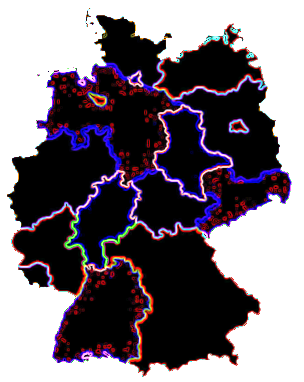
\includegraphics[width=0.2\textwidth]{Figures/MapUnColored.png}
  \hspace{0.5cm}
  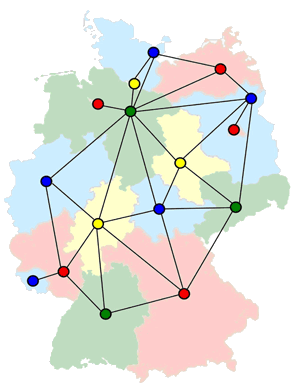
\includegraphics[width=0.2\textwidth]{Figures/MapColored.png}
\end{center}

La respuesta está dada por el número cromático del grafo de la derecha, donde cada vértice representa una región y dos vértices están conectados si las regiones que representan son limítrofes.s.



\section{Grafos planares}

El estudio de coloraciones mínimas está fuertemente ligado a las propiedades geométricas de los grafos, en particular, a su representación en el plano.

\begin{definitionblock}{Grafo planar}
Un grafo es \textbf{planar} si y solo si puede dibujarse en el plano sin que sus aristas se crucen.
\end{definitionblock}

\bigskip

Una representación planar de un grafo divide al plano en \textbf{regiones}, que son las zonas delimitadas por las aristas del grafo cuando este se dibuja en el plano sin cruces. Entre estas regiones siempre se encuentra una región no acotada o exterior, que rodea completamente al dibujo.

Cada vez que una arista o conjunto de aristas encierran una parte del plano sin cruzarse entre sí, forman una región distinta. El número de regiones en una representación planar depende de cómo se conecta el grafo y cuántas aristas y vértices contiene, pero no de cómo se dibuje, siempre que sea una representación planar válida.

Estas regiones son clave en el estudio topológico de grafos, ya que permiten aplicar la fórmula de Euler. También son útiles en aplicaciones como mapas o circuitos, donde evitar cruces mejora la claridad y funcionalidad del diseño.



\begin{exampleblock}{Ejemplo}
La siguiente representación planar divide el plano en 6 regiones:
\begin{center}
\begin{tikzpicture}[scale=0.8, every node/.style={circle, draw, fill=black, inner sep=1pt, minimum size=3pt}]
  % Nodes
  \node (A) at (0,0) {};
  \node (B) at (2,0) {};
  \node (C) at (4,0) {};
  \node (D) at (0,2) {};
  \node (E) at (2,2) {};
  \node (F) at (4,2) {};
  \node (G) at (2,-2) {};
  \node (H) at (4,-2) {};

  % Edges
  \draw (A) -- (B) -- (C);
  \draw (D) -- (E) -- (F);
  \draw (A) -- (D);
  \draw (B) -- (E);
  \draw (C) -- (F);
  \draw (B) -- (G);
  \draw (C) -- (H);
  \draw (G) -- (H);
  \draw (A) -- (G);
  \draw (E) -- (C);

  % Region labels
  \node[draw=none, fill=none, text=blue] at (1.,1) {$R_1$};
  \node[draw=none, fill=none, text=blue] at (1.2,-0.5) {$R_2$};
  \node[draw=none, fill=none, text=blue] at (2.6,0.5) {$R_3$};
  \node[draw=none, fill=none, text=blue] at (3.3,1.3) {$R_4$};
  \node[draw=none, fill=none, text=blue] at (3,-0.8) {$R_5$};
  \node[draw=none, fill=none, text=blue] at (4.5,0) {$R_6$};
\end{tikzpicture}
\end{center}
\end{exampleblock}


\subsection{Aplicación: Diseño de circuitos eléctricos}

Una aplicación fundamental de los grafos planares se encuentra en el diseño de circuitos eléctricos y microprocesadores. En estos contextos, los componentes electrónicos y sus conexiones se modelan mediante grafos, donde los vértices representan nodos de conexión y las aristas los conductores o enlaces físicos.

\medskip

Para minimizar costos y evitar interferencias, es crucial que el diseño del circuito sea \textbf{planar}, es decir, que las conexiones puedan trazarse en una sola capa sin que se crucen. Si un grafo no es planar, se requieren capas adicionales o el uso de tecnología más costosa para separar conexiones cruzadas.

\begin{center}
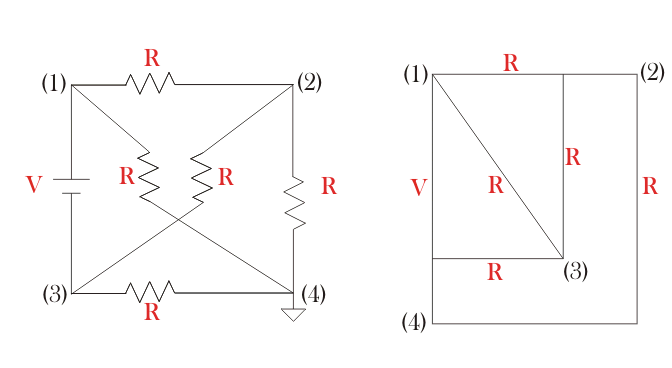
\includegraphics[width=0.5\textwidth]{Figures/planar_circuit.png}
\end{center}

Este problema motiva algoritmos para el reconocimiento de grafos planares y su embebido en el plano.



\subsection{Fórmula de Euler}

Leonhard Euler descubrió una relación entre el número de vértices, aristas y regiones en cualquier grafo planar, conexo y sin múltiples aristas ni lazos. Esta relación es conocida como la \textbf{fórmula de Euler}.


\begin{thmblock}{Fórmula de Euler}
Sea \( G = (V,E) \) un grafo simple, conexo y planar. Sea \( r \) el número de regiones en una representación planar de \( G \). Entonces:
\[
r = |E| - |V| + 2
\]

Esta fórmula es válida para cualquier representación planar del grafo, sin importar su disposición geométrica específica.
\end{thmblock}
\begin{proof}
La demostración se realiza por inducción sobre el número de aristas.
Construimos una secuencia de subgrafos planares:
\[
G_1, G_2, \dots, G_{|E|}
\]
donde cada \( G_{j+1} \) se obtiene al agregar una arista de \( G \) a \( G_j \), de forma que se mantenga la conexidad. Como \( G \) es conexo, siempre podemos agregar una arista que se conecte con los vértices ya presentes.

Demostraremos por inducción que todo \( G_j = (V_j, E_j) \) cumple:
\[
r_j = |E_j| - |V_j| + 2
\]
siendo \( r_j \) el número de regiones de su representación planar.

\textbf{Caso base:} \( G_1 \) tiene una sola arista y dos vértices. Como no encierra ninguna región, \( r_1 = 1 \), y:
\[ r_1 = 1 = 1 - 2 + 2 = 1 \checkmark \]

\textbf{Paso inductivo:} Al agregar una nueva arista, se presentan dos casos:
\begin{itemize}
  \item[(1)] Si une dos vértices ya presentes, crea una nueva región: \( r_{j+1} = r_j + 1 \), \( E_{j+1} = E_j + 1 \) y \( V_{j+1} = V_j \).
  $$\therefore \ {r_{j+1} = |E_{j+1}| - |V_{j+1}| + 2}.$$ 
  \item[(2)] Si introduce un nuevo vértice, no crea regiones: \( r_{j+1} = r_j \), \( E_{j+1} = E_j + 1 \) y \( V_{j+1} = V_j + 1 \).
  $$\therefore \ {r_{j+1} = |E_{j+1}| - |V_{j+1}| + 2}.$$
\end{itemize}

En ambos casos se mantiene:
\[
r_{j+1} = |E_{j+1}| - |V_{j+1}| + 2 \quad \checkmark
\]

Por lo tanto, por inducción, la fórmula se cumple para \( G \).
\end{proof}


\begin{exampleblock}{Ejemplo de Fórmula de Euler}
En el grafo del ejemplo anterior:
\begin{itemize}
  \item Número de vértices: \( |V| = 8 \)
  \item Número de aristas: \( |E| = 12 \)
  \item Número de regiones: \( r = 6 \)
\end{itemize}

Verifiquemos la fórmula:
\[ r = |E| - |V| + 2 = 12 - 8 + 2 = 6 \quad \checkmark \]

La fórmula se cumple.
\end{exampleblock}

\subsection{Corolarios de la fórmula de Euler}
El primer corolario que estudiaremos establece una cota superior para el número de arcos de un grafo planar.
\begin{thmblock}{Corolario 1}
Si \( G \) es un grafo simple, conexo y planar con \( |V| \geq 3 \), entonces:
\[
|E| \leq 3|V| - 6
\]
\end{thmblock}

El siguiente corolario establece una condición necesaria de planaridad.
\begin{thmblock}{Corolario 2}
Todo grafo simple, conexo y planar tiene al menos un vértice de grado a lo sumo 5.
\end{thmblock}

\subsection*{Ejercicios propuestos}

\begin{enumerate}
  \item  Demostrar que el grafo completo \( K_5 \) no es planar.

  \item Sea \( G \) un grafo simple y planar con 9 vértices. ¿Cuál es el máximo número posible de aristas que puede tener?
  \item Da un ejemplo de un grafo conexo que cumple \( |E| \leq 3|V| - 6 \) pero no es planar. ¿Es esto posible?
  \item{*}Demuestra que el grafo bipartito completo \( K_{3,3} \) no es planar, utilizando una variante del Corolario 1 para grafos con ciclos de longitud $\geq4$.
%   \begin{proof} Como en toda representación planar, la suma de los grados de las regiones es igual a dos veces el número de aristas:
% \[
% \sum \deg(R_i) = 2|E|
% \]
% Pero si todos los ciclos tienen longitud \( \geq 4 \), entonces cada región está delimitada por al menos 4 aristas, por lo que:
% \[
% 4|F| \leq 2|E| \Rightarrow 2|F| \leq |E|
% \]
% Aplicando la fórmula de Euler \( |V| - |E| + |F| = 2 \), despejamos \( |F| = |E| - |V| + 2 \) y sustituimos:
% \[
% 2(|E| - |V| + 2) \leq |E| \Rightarrow 2|E| - 2|V| + 4 \leq |E| \Rightarrow |E| \leq 2|V| - 4
% \]
% \end{proof}

\end{enumerate}


\section{Teorema de los Cuatro Colores}

Uno de los resultados más sorprendentes y célebres de la teoría de grafos es el llamado \textbf{Teorema de los Cuatro Colores}. Este surge al estudiar la coloración de grafos planares.

La respuesta, aunque simple, tardó más de un siglo en ser formalmente demostrada.

\begin{thmblock}{Teorema de los Cuatro Colores \textit{(Appel \& Haken, 1976)}}
Sea \( G \) un grafo simple, conexo y planar. Entonces:
\[
\chi(G) \leq 4
\]
Es decir, todo grafo planar puede ser coloreado usando a lo sumo cuatro colores.
\end{thmblock}

Este resultado implica que cualquier mapa, por complejo que sea, puede colorearse con cuatro colores de modo que regiones adyacentes no compartan el mismo color.

\subsection*{Breve historia del teorema}

La conjetura fue planteada en 1852 por Francis Guthrie. A pesar de múltiples intentos fallidos de demostración, no fue hasta 1976 que Kenneth Appel y Wolfgang Haken lograron una prueba definitiva, aunque controversial, utilizando asistencia computacional.

\paragraph{La idea de la demostración.}
Appel y Haken demostraron que no puede existir un \textbf{contraejemplo minimal} al teorema. Para ello, redujeron la verificación a 1.936 configuraciones críticas, las cuales fueron examinadas mediante un algoritmo computacional que corrió durante cientos de horas.

La parte teórica de su demostración ocupa más de 500 páginas, con análisis manual de \textit{contra-contra-ejemplos}. Muchos de estos fueron revisados por el propio hijo de Haken.

El método de demostración generó debate en la comunidad matemática por dos razones. Primero, una parte clave de la prueba fue verificada únicamente por computadora, lo que en su momento generaba desconfianza.
Segundo, la porción escrita a mano era demasiado extensa y engorrosa para que alguien la verificara por completo.


\paragraph{Segunda prueba (Robertson et al., 1997)}

En 1997, Robertson, Sanders, Seymour y Thomas publicaron una nueva prueba del Teorema de los Cuatro Colores en la revista \textit{Journal of Combinatorial Theory}. Esta sigue la misma estrategia general de Appel y Haken, pero con importantes mejoras, por ejemplo, el número de configuraciones se redujo a 633.


\paragraph{Estado actual.} Hasta hoy, no se conoce una demostración del teorema que pueda ser completamente verificada sin asistencia computacional. Aun así, el resultado se acepta universalmente como verdadero, y marca un hito en el uso de computadoras para la demostración matemática.


\subsection{Teoremas de coloración débil para grafos planares}

Además del Teorema de los Cuatro Colores, existen versiones más accesibles que se pueden demostrar con técnicas elementales.

\begin{thmblock}{6-coloración}
Sea \( G \) un grafo simple, conexo y planar. Entonces:
\[ \chi(G) \leq 6 \]
\end{thmblock}

\begin{proof} Por inducción en el número de vértices \( n \).

\textbf{Caso base:} Para \( n \leq 6 \), coloreamos cada vértice con un color distinto.

\textbf{Hipótesis inductiva (HI):} Supongamos que todo grafo planar con \( n-1 \) vértices es 6-colorable.

Sea \( G \) un grafo planar con \( n \) vértices. Por el Corolario del Teorema de Euler, existe un vértice \( v \) de grado a lo sumo 5.

Eliminamos \( v \) y sus aristas incidentes. El grafo restante tiene \( n-1 \) vértices y es 6-colorable por HI.

Entonces podemos colorear \( v \) con un color distinto al de sus (a lo sumo) 5 vecinos.
\end{proof}

\begin{thmblock}{5-coloración}
Sea \( G \) un grafo simple, conexo y planar. Entonces:
\[ \chi(G) \leq 5 \]
\end{thmblock}

\begin{proof}
La demostración también se basa en inducción, pero requiere análisis más delicado sobre cómo intercambiar colores entre vecinos de un nodo \( v \) de grado 5.

\textbf{Caso base:} Todo grafo planar con \( n \leq 5 \) es trivialmente 5-colorable.

\textbf{Hipótesis inductiva (HI):} Todo grafo simple, conexo y planar con \( n-1 \) vértices es 5-colorable.

Sea \( G \) un grafo con \( n \) vértices. Por el Corolario del Teorema de Euler, existe un vértice \( v \) de grado a lo sumo 5. Eliminamos \( v \) y sus aristas incidentes. Por HI, el grafo restante se puede colorear con 5 colores.

Si \( v \) tiene menos de 5 vecinos, al menos un color está disponible para colorearlo. El caso crítico ocurre cuando \( v \) tiene exactamente 5 vecinos con 5 colores distintos.

\begin{center}
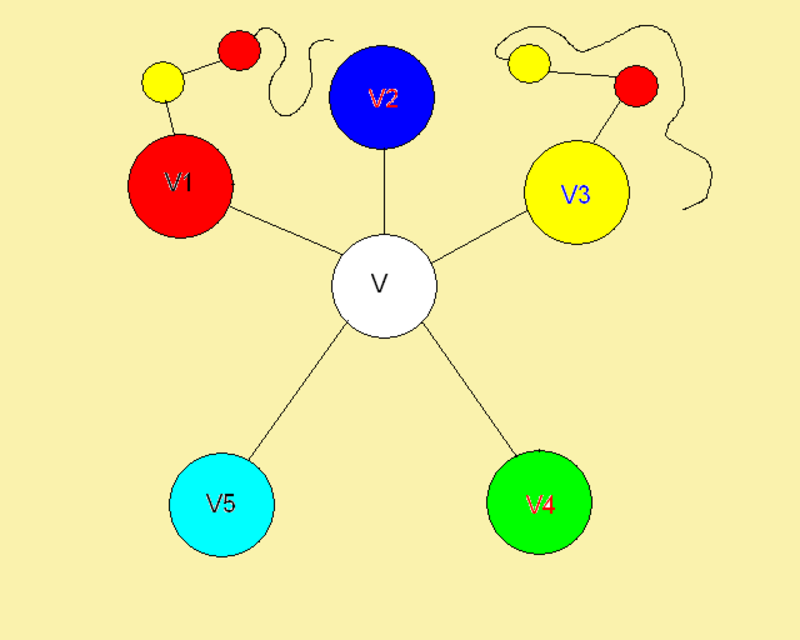
\includegraphics[width=0.3\textwidth]{Figures/fig5color_1}
\end{center}

Sea \( v_1, v_2, v_3, v_4, v_5 \) los vecinos de \( v \), cada uno con un color distinto. Si en el subgrafo inducido por los vecinos, dos vértices con colores \textit{rojo} y \textit{amarillo} (digamos \( v_1 \) y \( v_3 \)) están en componentes diferentes, se puede intercambiar rojo y amarillo en el componente de \( v_1 \), liberando un color para \( v \).

\begin{center}
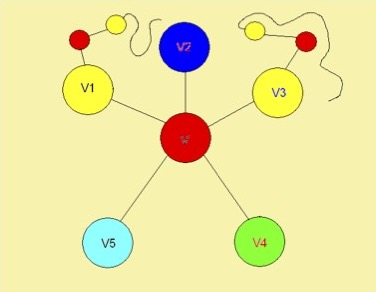
\includegraphics[width=0.3\textwidth]{Figures/fig5color_2}
\end{center}

Si hay un camino entre \( v_1 \) y \( v_3 \), se puede intentar intercambiar otros pares de colores, como \textit{verde} y \textit{azul}:

\begin{center}
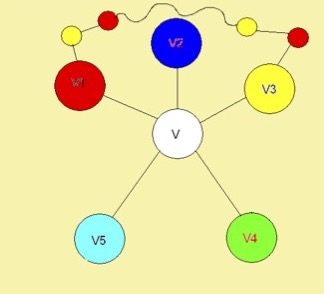
\includegraphics[width=0.3\textwidth]{Figures/fig5color_3}
\end{center}

En el caso extremo en que hay caminos entre \( v_1 \) y \( v_3 \), y también entre \( v_2 \) y \( v_4 \), los caminos deben cruzarse. Esto contradice la planaridad del grafo:

\begin{center}
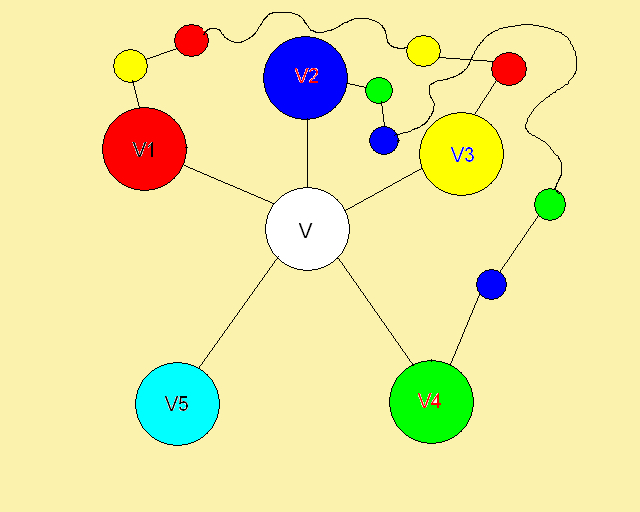
\includegraphics[width=0.35\textwidth]{Figures/fig5color_4}
\end{center}

Por lo tanto, uno de los intercambios de colores es siempre posible, y \( v \) puede ser coloreado con un color distinto a sus vecinos. Esto completa la prueba.
\end{proof}



% \title{Apunte de Matemáticas Discretas CC3101:\\ 
%   Introducción a Árboles Clase 22}
% % \title{Ejercicios Lógica e Inducción}
% \author{Andrés Abeliuk}
% \date{}
% \maketitle

\section{Árboles}

\subsection{Motivación e historia}

Los árboles son estructuras fundamentales en matemáticas discretas y ciencias de la computación. Representan relaciones jerárquicas y son usadas en estructuras de datos, algoritmos, lenguajes de programación, bases de datos y más.

El término “árbol” fue introducido por Arthur Cayley en el siglo XIX para contar estructuras moleculares. Desde entonces, se ha convertido en un concepto central en teoría de grafos.

\subsection{¿Qué es un árbol?}

\begin{definitionblock}{Árbol}
Un \textbf{árbol} es un grafo no dirigido que es \emph{conexo} y \emph{acíclico}. Es decir, existe un camino entre todo par de vértices, y no contiene ciclos simples.
\end{definitionblock}

\noindent \textbf{Observación:} Todo árbol debe ser necesariamente un grafo simple (es decir, sin lazos ni aristas paralelas).


\begin{center}
\begin{tikzpicture}[scale=1.2, every node/.style={circle, draw, fill=white}]
\node (a) at (0,0) {a};
\node (b) at (-1,-1) {b};
\node (c) at (1,-1) {c};
\node (d) at (-1.5,-2) {d};
\node (e) at (-0.5,-2) {e};
\node (f) at (1.5,-2) {f};

\draw (a) -- (b);
\draw (a) -- (c);
\draw (b) -- (d);
\draw (b) -- (e);
\draw (c) -- (f);
\end{tikzpicture}
\end{center}

\subsection{Ejemplos y contraejemplos}

\begin{exampleblock}{¿Cuáles de los siguientes grafos son árboles?}
\begin{center}
\begin{tikzpicture}[scale=1, every node/.style={circle, draw, inner sep=1pt, font=\footnotesize}]
% G1
\node (a1) at (0,2) {a};
\node (b1) at (1,2) {b};
\node (c1) at (0.5,1) {c};
\node (d1) at (1.5,1) {d};
\node (e1) at (0,0) {e};
\node (f1) at (1,0) {f};
\draw (a1) -- (c1);
\draw (b1) -- (c1);
\draw (c1) -- (d1);
\draw (c1) -- (e1);
\draw (e1) -- (f1);
\node[draw=none, fill=none] at (0.75,-0.5) {$G_1$};

% G2
\begin{scope}[xshift=3.5cm]
\node (a2) at (0,2) {a};
\node (b2) at (1,2) {b};
\node (c2) at (0,1) {c};
\node (d2) at (1,1) {d};
\node (e2) at (0,0) {e};
\node (f2) at (1,0) {f};
\draw (a2) -- (e2);
\draw (b2) -- (f2);
\draw (c2) -- (f2);
\draw (e2) -- (f2);
\node[draw=none, fill=none] at (0.5,-0.5) {$G_2$};
\end{scope}

% G3
\begin{scope}[xshift=7cm]
\node (a3) at (0,2) {a};
\node (b3) at (1,2) {b};
\node (c3) at (0,1) {c};
\node (d3) at (1,1) {d};
\node (e3) at (0,0) {e};
\node (f3) at (1,0) {f};
\draw (a3) -- (b3);
\draw (a3) -- (d3);
\draw (c3) -- (e3);
\draw (c3) -- (f3);
\draw (e3) -- (b3);
\node[draw=none, fill=none] at (0.5,-0.5) {$G_3$};
\end{scope}

% G4
\begin{scope}[xshift=10.5cm]
\node (a4) at (0,2) {a};
\node (b4) at (1,2) {b};
\node (c4) at (0,1) {c};
\node (d4) at (1,1) {d};
\node (e4) at (0,0) {e};
\node (f4) at (1,0) {f};
\draw (a4) -- (f4);
\draw (b4) -- (d4);
\draw (c4) -- (e4);
\node[draw=none, fill=none] at (0.5,-0.5) {$G_4$};
\end{scope}
\end{tikzpicture}
\end{center}
\end{exampleblock}

\subsection{Aplicaciones de los árboles}

Los árboles son útiles en múltiples contextos, como se muestra a continuación:

\begin{itemize}
  \item \textbf{Búsqueda y ordenamiento:} Los \emph{árboles binarios de búsqueda} (BST) permiten organizar datos de forma que cada nodo tiene a lo sumo dos hijos. El hijo izquierdo contiene valores menores y el derecho, mayores. Esto permite búsquedas, inserciones y eliminaciones en tiempo promedio \( O(\log n) \), si el árbol está balanceado. Son usados en estructuras de datos como sets, maps y en bases de datos.

  \item \textbf{Compresión de datos:} El algoritmo de \emph{Huffman} construye un árbol binario donde cada hoja representa un símbolo, y la ruta desde la raíz define su código binario. Los símbolos más frecuentes tienen códigos más cortos, minimizando la longitud promedio del mensaje. Estos árboles son fundamentales en formatos como JPEG, MP3 y ZIP.


  \item \textbf{Modelado de juegos:} En teoría de juegos, los árboles modelan todos los posibles estados y jugadas. Cada nodo representa un estado, y las ramas, movimientos. Son esenciales en juegos como ajedrez o tic-tac-toe. Algoritmos como \emph{minimax} y \emph{poda alfa-beta} operan sobre estos árboles para decidir jugadas óptimas.

\begin{center}
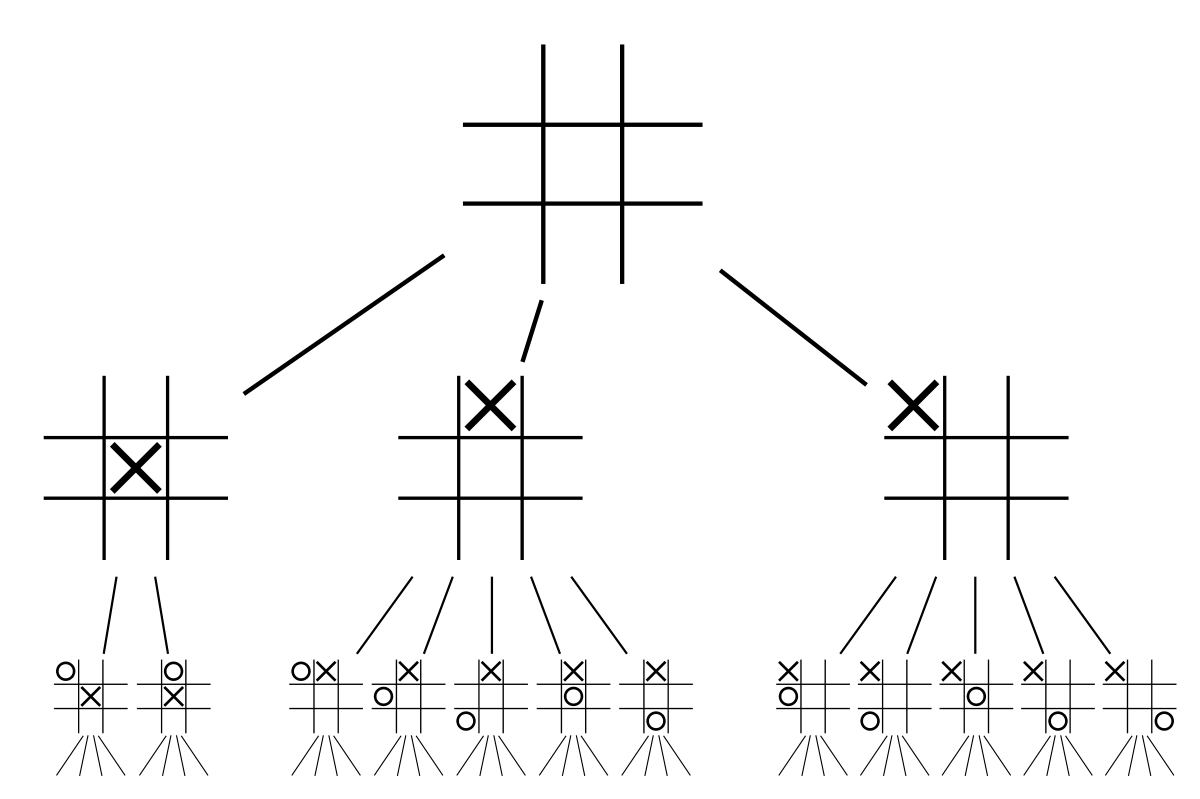
\includegraphics[width=0.45\textwidth]{Figures/tictactoetree.png}
\end{center}
\begin{center}\small\textit{Figura: Árbol de decisiones del juego Tic-Tac-Toe.}\end{center}

  \item \textbf{Estructuración de información:} Formatos como \emph{XML} y \emph{JSON} representan información anidada de forma jerárquica usando árboles. Cada nodo es una etiqueta o clave, y sus hijos representan contenido anidado. Esto facilita la consulta (e.g. con XPath), la transformación, y la validación de documentos.

  \item \textbf{Representación de decisiones:} En \emph{machine learning}, los árboles de decisión modelan decisiones mediante tests secuenciales sobre los datos. Cada nodo representa una pregunta; las ramas, respuestas posibles; y las hojas, una predicción. Son la base de modelos como CART, Random Forest y XGBoost, destacándose por su interpretabilidad.
\end{itemize}

% \subsubsection*{Árbol binario de búsqueda (BST)}

% \begin{center}
% \begin{tikzpicture}[level distance=1.2cm,
%   level 1/.style={sibling distance=2.8cm},
%   level 2/.style={sibling distance=1.4cm},
%   every node/.style={circle, draw}]
% \node {8}
%   child {node {3}
%     child {node {1}}
%     child {node {6}}}
%   child {node {10}
%     child[missing]
%     child {node {14}}};
% \end{tikzpicture}
% \end{center}

% \subsubsection*{Códigos de Huffman}

% \begin{center}
% \begin{tikzpicture}[sibling distance=8mm,
%   level distance=10mm,
%   every node/.style = {circle, draw, font=\tiny}]
% \node { }
%   child {node {a}}
%   child {node { }
%     child {node {b}}
%     child {node { }
%       child {node {c}}
%       child {node {d}}}};
% \end{tikzpicture}
% \end{center}

% \textbf{Ventaja:} el código es \emph{prefix-free} (ningún código es prefijo de otro), lo que permite decodificar sin ambigüedad.



\begin{center}
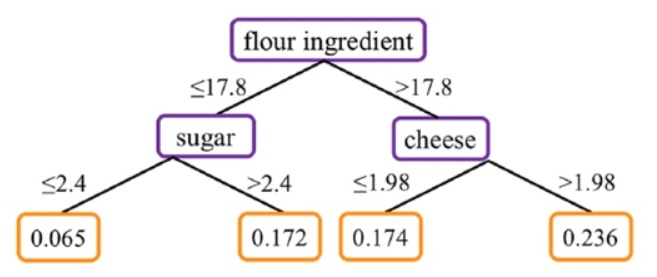
\includegraphics[width=0.5\textwidth]{Figures/tree_food_crop}
\end{center}
\begin{center}\small\textit{Figura: Árbol de regresión con tres predictores (harina, azúcar y queso), utilizado para clasificar países según su consumo y predecir prevalencia de obesidad en cuatro grupos distintos.
 Fuente: Dunstan, J., et al. (2020). Predicting nationwide obesity from food sales using machine learning.}\end{center}



\subsection{Caracterizaciones alternativas}


A primera vista, la definición de árbol puede parecer un tanto arbitraria: un grafo que es \emph{conexo} y \emph{acíclico}. Pero, ¿por qué esas dos condiciones en particular? Para responder esta pregunta, es útil considerar qué implican esas propiedades en términos de la estructura del grafo.

\textbf{Conexión} significa que hay un camino entre cada par de nodos. Es decir, el grafo debe tener suficientes aristas para mantener todos los vértices conectados en una sola componente. Por otro lado, \textbf{no tener ciclos} nos obliga a restringir el número de conexiones: no puede haber más aristas que las necesarias, porque cualquier exceso podría cerrar un ciclo.

Los árboles, entonces, se sitúan exactamente en el \emph{punto de equilibrio} entre tener suficientes aristas para ser conexos, pero no tantas como para crear ciclos. Este balance permite que muchas propiedades estructurales equivalentes emerjan, como veremos en el siguiente teorema.


\begin{exampleblock}{Teorema}
Sea $G=(V,E)$ un grafo no dirigido. Las siguientes propiedades son equivalentes:
\begin{enumerate}
  \item $G$ es un árbol;
  \item $G$ contiene un único camino simple entre cada par de nodos distintos;
  \item $G$ es conexo y $|E| = |V| - 1$.
\end{enumerate}
\end{exampleblock}

\subsubsection*{Demostraciones}

\paragraph{1 $\Rightarrow$ 2:} Sea $u$ y $v$ vértices distintos de $G$. Como $G$ es un árbol, es conexo y por lo tanto existe un camino simple que los conecta. 

Supongamos que hay dos caminos simples distintos entre $u$ y $v$: $C_1$ y $C_2$. Esto implicaría la existencia de un ciclo simple en $G$, contradiciendo la hipótesis.

Si divergen antes de finalizar, los caminos generan un ciclo entre el primer punto de divergencia $x$ y el de reencuentro $y$:
\begin{center}
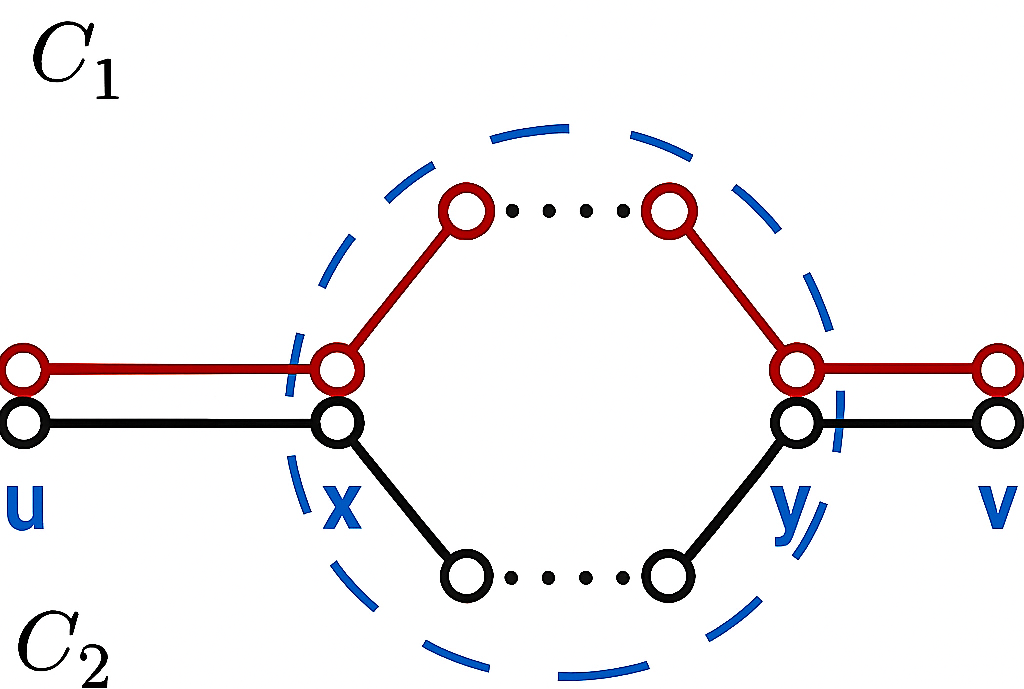
\includegraphics[width=0.35\textwidth]{Figures/ciclo.png}
\end{center}

\paragraph{2 $\Rightarrow$ 1:} Por hipótesis, existe un único camino simple entre cada par de nodos. Esto implica que $G$ es conexo. Supongamos ahora que $G$ contiene un ciclo simple. Entonces, entre dos nodos de ese ciclo hay más de un camino simple, contradiciendo la unicidad. \hfill $\square$

\paragraph{1 $\Rightarrow$ 3:} Demostración por inducción fuerte sobre $|E|$.

\textit{HI:} Para todo árbol con $|E| \leq d$, se cumple $|E| = |V| - 1$.

Consideremos un árbol cualquiera $G$ con $|E| = d + 1$.  Sea  $G\setminus{a}$ el grafo que se forma quitando de $G$ la arista $a$ tal que el árbol no es conexo,  i.e.,  $G\setminus{a}= G_1 \cup G_2$,  donde $G_1$ y $G_2$ son árboles con no más de $d$ aristas.
Por la caracterización 2, toda arista es esencial: si se elimina, el grafo se desconecta.

Aplicamos a $G_1$ y $G_2$ la HI: $|E(G_i)|=|V_i|-1$ y sumando obtenemos  $|E| - 1 = (|V_1| - 1) + (|V_2| - 1) = |V| - 2$, por lo tanto $|E| = |V| - 1$.
\hfill $\square$

\paragraph{3 $\Rightarrow$ 1:} Supongamos que $G$ es conexo y $|E| = |V| - 1$, pero que contiene un ciclo. Eliminamos una arista del ciclo. El nuevo grafo $G'$ sigue siendo conexo pero ahora tiene $|E| < |V| - 1$,  lo cual es imposible.

De hecho, \textbf{todo grafo conexo debe tener al menos $|V| - 1$ aristas}, pues de lo contrario no es posible conectar todos los vértices.
\hfill $\square$


\subsection{Árboles con raíz}

En muchas aplicaciones es útil distinguir un nodo particular como la \textbf{raíz} del árbol. A menudo, en los \textbf{árboles con raíz} se orientan las aristas para que apunten \emph{lejos} de la raíz.

\begin{center}
\begin{tikzpicture}[->, every node/.style={circle, draw}, level distance=1.2cm, sibling distance=1.4cm]
\node (a) {a}
  child {node (b) {b}
    child {node {f}}
    child {node {g}}}
  child {node (c) {c}
    child {node {e}}}
  child {node {d}};
\end{tikzpicture}
\end{center}

\subsection*{Terminología básica}
Sea $T$ un árbol con raíz $v$:
\begin{itemize}
  \item El \textbf{padre} de un nodo $u \neq v$ es el vértice desde el cual se llega a $u$ por una arista dirigida. A su vez, $u$ es un \textbf{hijo} de ese vértice.
  \item Dos nodos son \textbf{hermanos} si tienen el mismo padre.
  \item Los \textbf{ancestros} de $u$ son los nodos en el camino desde $u$ hacia la raíz. Sus \textbf{descendientes} son los nodos que tienen a $u$ como ancestro.
  \item Una \textbf{hoja} es un nodo sin hijos; los demás se llaman \textbf{internos}.
  \item La \textbf{altura} del árbol es la longitud del camino más largo desde la raíz hacia cualquier hoja.
\end{itemize}

\subsection{Árboles $m$-arios}

A veces interesa restringir la cantidad de hijos que puede tener un nodo.

\begin{exampleblock}{Definición}
Un árbol con raíz es \textbf{$m$-ario} ($m \geq 1$) si cada nodo interno tiene a lo más $m$ hijos. Es \textbf{completo} si todos los nodos internos tienen exactamente $m$ hijos.
\end{exampleblock}

\begin{center}
\begin{tikzpicture}[level distance=1.2cm,
  level 1/.style={sibling distance=2.4cm},
  level 2/.style={sibling distance=1.2cm},
  every node/.style={circle, draw}]
\node {A}
  child {node {B}
    child {node {D}}
    child {node {E}}}
  child {node {C}
    child {node {F}}
    child {node {G}}};
\end{tikzpicture}
\end{center}

\subsection*{Propiedades fundamentales}
\begin{exampleblock}{Teorema}
\begin{itemize}
  \item Si $T$ es un árbol $m$-ario de altura $h$, entonces tiene a lo sumo $m^h$ hojas.
  \item Si $T$ es un árbol $m$-ario completo con $i$ nodos internos, entonces tiene $m \cdot i + 1$ nodos en total.
\end{itemize}
\end{exampleblock}

\subsection*{Ejercicios}

\newboxquestion{P1} Sea $G$ un grafo no dirigido. Probar que $G$ es un árbol si y sólo si $G$ es conexo, pero sacarle cualquier arista lo vuelve disconexo.
\begin{proof}
\leavevmode

\paragraph{\( \Rightarrow \)}
Asuma que $G = (V, E)$ es un árbol. Queremos probar que quitar cualquier arista lo desconecta.

\begin{itemize}
  \item Como $G$ es un árbol, es conexo por definición.
  \item Supongamos por contradicción que existe una arista $e \in E$ tal que el grafo $G' = (V, E \setminus \{e\})$ sigue siendo conexo.
  \item Entonces $G'$ sería un grafo conexo y sin ciclos (porque $G$ no tenía ciclos y quitar una arista no puede crear uno), es decir, también un árbol.
  \item Pero entonces: $|E| = |V| - 1$ y $|E \setminus \{e\}| = |V| - 2$, lo que contradice la caracterización 3.
\end{itemize}

\paragraph{ \( \Leftarrow \)}
Asuma que $G = (V, E)$ es conexo, y que quitar cualquier arista lo desconecta. Queremos probar que $G$ no tiene ciclos simples.

\begin{itemize}
  \item Supongamos por contradicción que $G$ contiene un ciclo simple $C$.
  \item Entonces podemos quitar una arista de $C$ y el grafo seguiría siendo conexo, ya que los vértices del ciclo seguirían conectados por el resto del ciclo.
  \item Esto contradice la hipótesis de que quitar cualquier arista desconecta $G$.
\end{itemize}

\end{proof}

\newboxquestion{P2} Demuestra que cualquier árbol es un grafo bipartito.


\begin{proof}
Como $T$ es un árbol, no contiene ciclos. Vamos a demostrar que $T$ es bipartito, es decir, que su conjunto de vértices $V$ se puede dividir en dos subconjuntos disjuntos $V_1$ y $V_2$ tal que ninguna arista conecta dos vértices dentro del mismo subconjunto.

Elegimos un vértice arbitrario $v \in V$ y definimos $V_1$ como el conjunto de vértices a distancia par de $v$ y $V_2$ como aquellos a distancia impar.

Como $T$ es un grafo sin ciclos, la distancia entre dos vértices cualesquiera está bien definida y única. Toda arista conecta dos vértices cuyas distancias respecto a $v$ difieren en exactamente 1 (ya que no hay ciclos), por lo que nunca une dos vértices ambos en $V_1$ ni ambos en $V_2$.

Por lo tanto, $T$ es bipartito.
\end{proof}

\newboxquestion{P3}  Ecuentre el número de árboles no isomórficos con 5 vértices

% \title{Apunte de Matemáticas Discretas CC3101:\\ 
%   Árboles generadores Clase 23}
% % \title{Ejercicios Lógica e Inducción}
% \author{Andrés Abeliuk}
% \date{}
% \maketitle

\section{Árboles Generadores}

\subsection{Motivación: Conectividad Mínima}

Supongamos que tenemos una red vial entre varias ciudades, en la que todas las rutas son caminos de tierra. Queremos pavimentar la menor cantidad posible de caminos, de modo que sea posible viajar entre cualquier par de ciudades usando sólo caminos pavimentados.

\begin{center}
\begin{tikzpicture}[scale=1, every node/.style={circle, draw, fill=gray!20, inner sep=2pt}]
  \foreach \i in {0,...,3} {
    \foreach \j in {0,...,3} {
      \node (v\i\j) at (\i,\j) {};
    }
  }
  \foreach \i in {0,...,3} {
    \foreach \j in {0,...,2} {
      \draw (v\i\j) -- (v\i\the\numexpr\j+1\relax);
    }
  }
  \foreach \i in {0,...,2} {
    \foreach \j in {0,...,3} {
      \draw (v\i\j) -- (v\the\numexpr\i+1\relax\j);
    }
  }
\end{tikzpicture}
\end{center}


\textbf{Pregunta:} ¿Cuál es la mínima cantidad de caminos que deben pavimentarse?


\medskip

La respuesta está dada por encontrar un subgrafo que conecte todas las ciudades (vértices) y no tenga ciclos. Este subgrafo es un \textbf{árbol generador} del grafo original.

\begin{center}
\begin{tikzpicture}[scale=1, every node/.style={circle, draw, fill=gray!20, inner sep=2pt}]
  \foreach \i in {0,...,3} {
    \foreach \j in {0,...,3} {
      \node (v\i\j) at (\i,\j) {};
    }
  }
  \draw (v00) -- (v01);
  \draw (v01) -- (v11);
  \draw (v11) -- (v12);
  \draw (v12) -- (v13);
  \draw (v12) -- (v02);
  \draw (v02) -- (v03);
  \draw (v00) -- (v10); 
  \draw (v10) -- (v20);
  \draw (v20) -- (v30); 
  \draw (v20) -- (v21);
  \draw (v21) -- (v31);
  \draw (v31) -- (v32);
  \draw (v32) -- (v33);
  \draw (v32) -- (v22);
  \draw (v22) -- (v23);
\end{tikzpicture}
\end{center}

\begin{definitionblock}{Árbol Generador}
Un \textbf{árbol generador} de un grafo $G = (V, E)$ es un subgrafo $T = (V, E')$ tal que:
\begin{itemize}
  \item $T$ contiene todos los vértices de $G$, es decir, $V(T) = V(G)$.
  \item $T$ es un árbol: está conectado y no contiene ciclos.
\end{itemize}
\end{definitionblock}


Este tipo de subgrafo no es único: un mismo grafo puede admitir múltiples árboles generadores diferentes, dependiendo de qué aristas se elijan para mantener la conectividad y evitar los ciclos.


\begin{exampleblock}{Ejemplo: Dos árboles generadores distintos del mismo grafo. }

\begin{center}
\begin{tikzpicture}[scale=1.2, every node/.style={circle, draw, fill=gray!20, inner sep=2pt}]
  \node (a) at (0,1) {};
  \node (b) at (1,2) {};
  \node (c) at (2,1) {};
  \node (d) at (1,0) {};

  \draw (a) -- (b);
  \draw (b) -- (c);
  \draw (c) -- (d);
  \draw[dashed, gray] (b) -- (d);
  \draw[dashed, gray] (d) -- (a);
  \draw[dashed, gray] (a) -- (c);
\end{tikzpicture}
\hspace{1cm}
\begin{tikzpicture}[scale=1.2, every node/.style={circle, draw, fill=gray!20, inner sep=2pt}]
  \node (a) at (0,1) {};
  \node (b) at (1,2) {};
  \node (c) at (2,1) {};
  \node (d) at (1,0) {};

  \draw (a) -- (b);
  \draw (b) -- (d);
  \draw[dashed, gray] (d) -- (c);
  \draw[dashed, gray] (a) -- (d);
  \draw (c) -- (a);
  \draw[dashed, gray] (b) -- (c);
\end{tikzpicture}
\end{center}
\end{exampleblock}

\medskip

\begin{center}
  % \includegraphics[width=0.5\textwidth]{SpanningTreeExample.png}
\end{center}

\subsubsection{Aplicación: Recorrido Eficiente}

Una aplicación clave de los árboles generadores es la de recorrer todos los vértices de un grafo de forma eficiente. Por ejemplo, un \textit{rastreador web} (web crawler), que recolecta datos para un motor de búsqueda, necesita visitar todos los documentos conectados por hipervínculos. Para lograrlo de manera eficiente, puede construirse un árbol generador del grafo de enlaces: este árbol permite visitar cada nodo exactamente una vez, garantizando así un recorrido completo en \textbf{tiempo lineal} respecto al número de vértices.



\subsection{Caracterización de Grafos que Admiten Árbol Generador}

Una vez comprendida la noción de árbol generador y su importancia para garantizar conectividad mínima sin redundancia, surge una pregunta natural: ¿qué condiciones debe cumplir un grafo para que sea posible extraerle un árbol generador? 


\begin{thmblock}{Teorema}
Un grafo $G$ admite un árbol generador si y sólo si es conexo.
\end{thmblock}

\begin{proof}
\textbf{($\Rightarrow$)} Si $G$ tiene un árbol generador, entonces $G$ debe ser conexo, porque un árbol conecta todos los vértices por definición.

\medskip

\textbf{($\Leftarrow$)} Sea $G$ un grafo conexo. Si $G$ ya es un árbol, entonces el resultado es inmediato. Si $G$ no es un árbol, entonces contiene al menos un ciclo simple. Podemos remover una arista de ese ciclo sin desconectar el grafo (porque sigue existiendo un camino entre los extremos de esa arista usando el resto del ciclo).

\medskip

Repetimos este proceso mientras haya ciclos: eliminamos una arista de algún ciclo simple. Este proceso debe terminar porque $G$ tiene un número finito de aristas, y cada vez eliminamos una. El resultado final es un subgrafo conexo sin ciclos, es decir, un árbol generador de $G$.
\end{proof}



\subsection{Construcción de Árboles Generadores}

La prueba anterior nos entrega un procedimiento para construir árboles generadores. Sin embargo, este método no es muy eficiente, ya que requiere identificar ciclos simples dentro del grafo. Afortunadamente, existen algoritmos más eficientes y ampliamente utilizados en la práctica para este propósito. Los más conocidos son:

\begin{itemize}
  \item \textbf{DFS (Depth First Search):} búsqueda en profundidad.
  \item \textbf{BFS (Breadth First Search):} búsqueda a lo ancho.
\end{itemize}

\subsubsection{Búsqueda en Profundidad (DFS)}

Dado un grafo no dirigido simple $G$, el algoritmo DFS parte desde un vértice inicial y avanza lo más lejos posible por cada rama antes de retroceder (\emph{backtracking}). De esta forma, se construye un camino largo sin repetir vértices hasta que ya no se pueda continuar, y luego se regresa al nodo anterior para explorar otras ramas.

\begin{center}
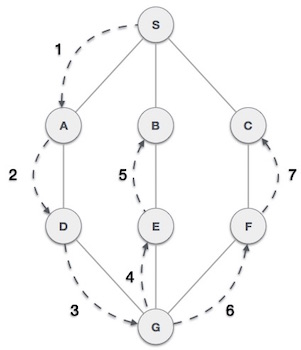
\includegraphics[width=0.25\textwidth]{Figures/DFS1.jpg}
\end{center}



\begin{exampleblock}{Algoritmo DFS}
\textbf{DFS}($G$ grafo conectado con vértices $v_1, v_2, \dots, v_n$):
\begin{itemize}
  \item[] $T$ := árbol que contiene solo el vértice $v_1$
  \item[] visita($v_1$)
\end{itemize}

\textbf{visita}($v$ vértice de $G$):
\begin{itemize}
  \item[] Para cada vértice $w$ adyacente a $v$ y no en $T$ hacer
  \begin{itemize}
    \item[] agregar $w$ y la arista $(v, w)$ a $T$
    \item[] visita($w$)
  \end{itemize}
\end{itemize}
\end{exampleblock}


\subsubsection*{Complejidad del DFS}

\begin{itemize}
  \item Cada vértice $v$ es visitado exactamente una vez: se llama al procedimiento \texttt{visita($v$)} cuando $v$ se encuentra por primera vez.
  \item Cada arista se examina como máximo dos veces: una desde cada uno de sus extremos.
  \item Por lo tanto, DFS tiene complejidad temporal $O(e)$ en representación por listas de adyacencia, o $O(n^2)$ en representación por matrices, donde $n$ es el número de vértices y $e$ el número de aristas.
\end{itemize}

\subsubsection{Búsqueda a lo Ancho (BFS)}

El algoritmo de búsqueda a lo ancho (BFS) también permite construir árboles generadores en grafos conexos. A diferencia del DFS, que explora lo más profundo posible antes de retroceder, el BFS explora todos los vecinos inmediatos de un nodo antes de continuar con los vecinos de esos vecinos, nivel por nivel.

\begin{center}
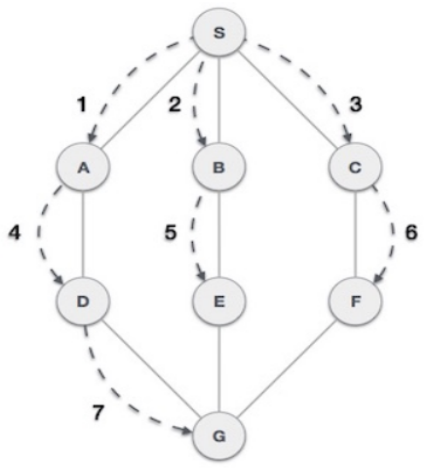
\includegraphics[width=0.25\textwidth]{Figures/BFS1.png}
\end{center}


\begin{exampleblock}{Algoritmo BFS}
\textbf{BFS}($G$ grafo conectado con vértices $v_1, v_2, \dots, v_n$):
\begin{itemize}
  \item[] $T$ := árbol que contiene solo el vértice $v_1$
  \item[] $Q$ := cola que contiene inicialmente solo $v_1$
  \item[] Mientras $Q$ no esté vacía hacer:
  \begin{itemize}
    \item[] $v$ := extraer primer elemento de $Q$
    \item[] Para cada vértice $w$ adyacente a $v$ y no en $T$ hacer
    \begin{itemize}
      \item[] agregar $w$ y la arista $(v, w)$ a $T$
      \item[] insertar $w$ al final de $Q$
    \end{itemize}
  \end{itemize}
\end{itemize}
\end{exampleblock}


\subsubsection*{Complejidad del BFS}

De manera análoga al análisis de DFS:

\begin{itemize}
  \item Cada vértice se visita exactamente una vez.
  \item Cada arista se examina como máximo dos veces: una vez desde cada uno de sus extremos.
  \item Por lo tanto, el algoritmo BFS también tiene una complejidad de $O(e)$ en representación con listas de adyacencia, o $O(n^2)$ con matrices de adyacencia, siendo $n$ el número de vértices y $e$ el número de aristas.
\end{itemize}


\subsection{Ejercicios Propuestos}

\begin{itemize}
  \item \textbf{Ejercicio:} Describa los árboles generadores producidos por los algoritmos DFS y BFS en una rueda $W_n$, comenzando por el vértice central.\\
  Una rueda $W_n$ es un grafo con $n$ vértices que se forma conectando un único vértice a todos los vértices de un ciclo-$(n-1)$.

  \item \textbf{Ejercicio:} Describa los árboles generadores producidos por los algoritmos DFS y BFS en un grafo completo $K_n$.

  \item \textbf{Ejercicio:} Sean $T$ y $T'$ dos árboles generadores del mismo grafo simple $G$. Asuma que existe un arco $e$ en $T$ que no pertenece a $T'$. Demuestre que existe un arco $e'$ en $T'$ tal que $e'$ no está en $T$, y tal que $T$ continúa siendo un spanning tree si le sacamos a $e$ y le agregamos a $e'$, y $T'$ continúa siendo un spanning tree si le sacamos a $e'$ y le agregamos a $e$.
\end{itemize}


\section{Árboles Generadores de Costo Mínimo}

\subsection{Definición y Motivación}

Si un grafo $G$ tiene costos asociados a cada arista, un problema natural es encontrar un árbol generador de \textbf{peso mínimo}. Esto significa hallar un subconjunto acíclico de aristas que conecte todos los vértices y cuya suma de pesos sea mínima.

\begin{definitionblock}{Árbol Generador de Peso Mínimo}
Dado un grafo simple $G$, un \textbf{árbol generador de peso mínimo} es un árbol generador de $G$ tal que la suma de los pesos de sus aristas es mínima.
\end{definitionblock}

\begin{center}
\tikzstyle{vertex}=[circle,fill=black!25,minimum size=20pt,inner sep=0pt]
\tikzstyle{selected vertex} = [vertex, fill=red!24]
\tikzstyle{edge} = [draw,thick,-]
\tikzstyle{weight} = [font=\small]
\tikzstyle{selected edge} = [draw,line width=5pt,-,red!50]
\tikzstyle{ignored edge} = [draw,line width=5pt,-,black!20]

\begin{tikzpicture}[scale=1.5, auto,swap]
    \foreach \pos/\name in {{(0,2)/a}, {(2,1)/b}, {(4,1)/c},
                            {(0,0)/d}, {(3,0)/e}, {(2,-1)/f}, {(4,-1)/g}}
        \node[vertex] (\name) at \pos {$\name$};

    % Edges (ignored first)
    \foreach \source / \dest in {d/b,d/e,e/f,b/c,f/g}
        \path[ignored edge] (\source.center) -- (\dest.center);

    % Edges (selected)
    \foreach \source / \dest in {d/a,d/f,a/b,b/e,e/c,e/g}
        \path[selected edge] (\source.center) -- (\dest.center);

    % Weights on top of everything
    \foreach \source/ \dest /\weight in {b/a/7, c/b/8,d/a/5,d/b/9,
                                         e/b/7, e/c/5,e/d/15,
                                         f/d/6,f/e/8,
                                         g/e/9,g/f/11}
        \path (\source) -- node[weight] {\weight} (\dest);

    % Selected vertices
    \foreach \vertex / \fr in {d/1,a/2,f/3,b/4,e/5,c/6,g/7}
        \node[selected vertex] at (\vertex) {$\vertex$};
\end{tikzpicture}
\end{center}


Hay dos algoritmos clásicos para encontrar árboles generadores mínimos: \textbf{Prim} y \textbf{Kruskal}.

\subsection{Algoritmo de Prim}

\begin{exampleblock}{Algoritmo de Prim}
Dado un grafo simple $G=(V,E)$, $n=|V|$, calcular el árbol de costo mínimo como sigue:
\begin{enumerate}
  \item Escoger el arco de \emph{menor peso} e incluirlo en el árbol.
  \item Repetidamente escoger el arco de menor peso incidente a un vértice existente del árbol, sin formar ciclos.
  \item Repetir hasta obtener $n-1$ aristas.
\end{enumerate}
\end{exampleblock}


\begin{center}
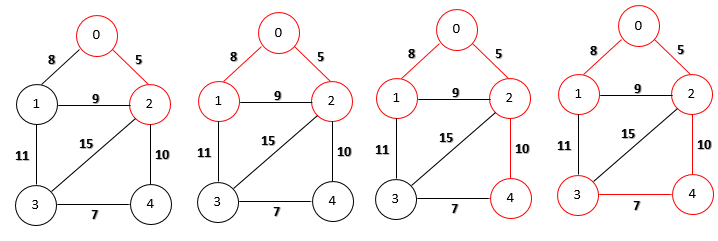
\includegraphics[scale=0.7]{Figures/Prim.png}
\end{center}



\subsection{Algoritmo de Kruskal}

\begin{exampleblock}{Algoritmo de Kruskal}
Dado un grafo simple $G=(V,E)$, $n=|V|$, calcular el árbol de costo mínimo como sigue:
\begin{enumerate}
  \item Ordenar las aristas por peso creciente.
  \item Añadir aristas una a una al árbol si no forman ciclos.
  \item Detenerse al obtener $n-1$ aristas.
\end{enumerate}
\end{exampleblock}

\begin{center}
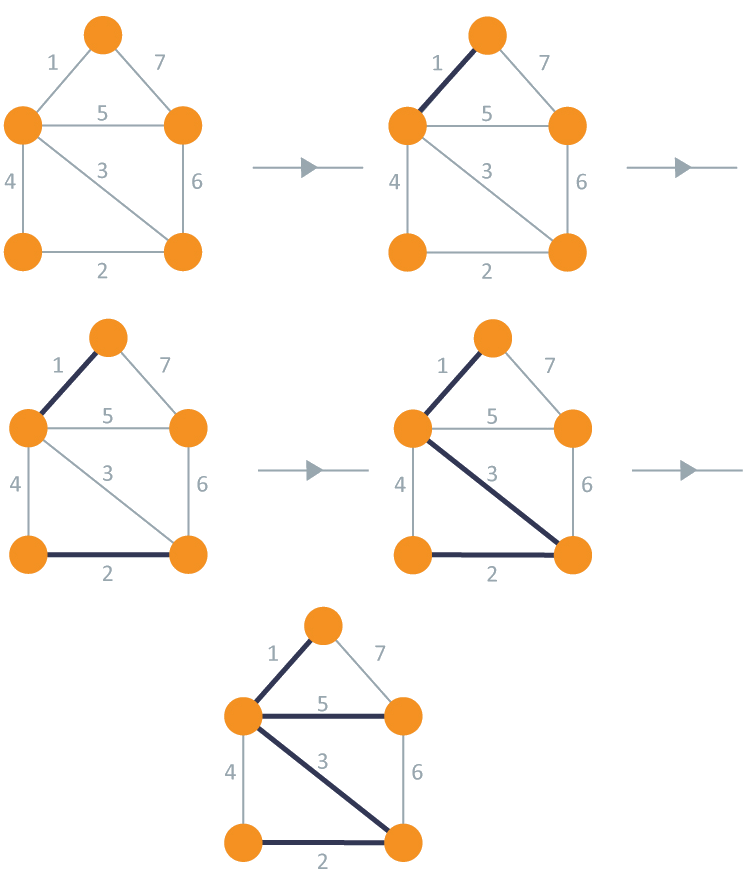
\includegraphics[scale=0.3]{Figures/Kruskal.png}
\end{center}


\subsection{Correctitud de los algoritmos}

Tanto Prim como Kruskal garantizan encontrar un árbol generador de peso mínimo. Sus demostraciones se basan en el principio del intercambio: si una arista no está en el árbol mínimo pero puede reemplazar otra sin aumentar el peso total, entonces el nuevo árbol sigue siendo mínimo.



\begin{thmblock}{Teorema (correctitud algoritmo Prim)}
 Dado un grafo simple $G=(V,E)$ de $n=|V|$ vértices y $e=|E|$ arcos, 
  el algoritmo de Prim encuentra un árbol generador de peso mínimo.
\end{thmblock}
\begin{proof}
Mostraremos la correctitud del algoritmo de Prim usando inducción matemática. Sea $T$ el conjunto de aristas seleccionadas por el algoritmo de Prim en cada iteración, y sea $M$ un árbol generador mínimo (MST).

\textbf{Hipótesis inductiva:} Después de cada iteración, el árbol parcial $T$ es un subgrafo de algún MST $M$.

\textbf{Caso base:} Al inicio, $T = \emptyset$, por lo tanto $T$ es un subgrafo de cualquier MST.

\textbf{Paso inductivo:} Supongamos que antes de una iteración, el árbol parcial $T$ es subgrafo de un MST $M$. Sea $e = (u,v)$ la arista que el algoritmo de Prim selecciona para agregar a $T$ en esta iteración. Como Prim solo añade aristas que conectan un vértice en $T$ con uno fuera, entonces $e$ conecta $T$ con el resto del grafo.

\begin{itemize}
  \item Si $e \in M$, entonces $T \cup \{e\}$ sigue siendo subgrafo de $M$, y la hipótesis se mantiene.
  \item Si $e \notin M$, entonces al agregar $e$ a $M$ se forma un ciclo, ya que $M$ es un árbol.
  \item En ese ciclo, debe existir otra arista $f$ que también conecta un vértice en $T$ con otro fuera de $T$.
  \item Como Prim eligió $e$ en vez de $f$, debe cumplirse que $w(e) \leq w(f)$.
  \item Al eliminar $f$ del ciclo y agregar $e$, obtenemos un nuevo árbol generador $M'$ cuyo peso total es menor o igual al de $M$, y que contiene a $T \cup \{e\}$.
\end{itemize}

Por lo tanto, por inducción, el árbol construido por Prim es un subgrafo de algún MST en cada paso, y al finalizar tiene $n-1$ aristas y conecta todos los nodos. Así, el árbol resultante es un MST.

\end{proof}



% \begin{proof}
% Sea $Y = e_1, \ldots, e_{n-1}$ el árbol generado por el algoritmo de Prim y sea $Y_1$ un árbol generador mínimo (MST).

% Si $Y \neq Y_1$, consideremos $e_k$ como la primera arista añadida durante la construcción de $Y$ que no pertenece a $Y_1$. Entonces, $Y_1$ contiene $e_1, \ldots, e_{k-1}$ pero no $e_k$.

% Sea $V$ el conjunto de vértices conectados por las aristas añadidas antes de $e_k$. Un extremo de $e_k$ está en $V$ y el otro fuera. Como $Y_1$ es un MST, existe un camino en $Y_1$ entre los extremos de $e_k$, y por lo tanto existe una arista $f$ en $Y_1$ que conecta $V$ con su complemento.

% En la iteración donde se eligió $e_k$, también se podría haber elegido $f$, lo cual implica:
% \[
%   w(f) \geq w(e_k)
% \]

% Sea $Y_2$ el grafo obtenido al reemplazar $f$ por $e_k$ en $Y_1$. Este nuevo grafo es también un árbol generador con peso total menor o igual al de $Y_1$, y contiene $e_k$. Repitiendo este procedimiento, obtenemos un MST que es idéntico al árbol $Y$.
% \end{proof}



\begin{thmblock}{Teorema (correctitud algoritmo Kruskal)}
Dado un grafo simple $G=(V,E)$ de $n=|V|$ vértices y $e=|E|$ arcos, 
  el algoritmo de Kruskal encuentra un árbol generador de peso mínimo.
\end{thmblock}

\paragraph{Propuesto: Demostrar correctitud del Algoritmo de Kruskal.}
La demostración de correctitud del algoritmo de Kruskal se basa en un argumento inductivo, similar al de Prim.

\subsection{Complejidad Algoritmos de Prim y Kruskal}

Dado un grafo simple $G = (V, E)$, el costo computacional de cada algoritmo es:

\begin{itemize}
  \item \textbf{Prim:} \stitle{$O(|E| \log |V|)$} \,\, (usando una cola de prioridad).
  \item \textbf{Kruskal:} \stitle{$O(|E| \log |E|)$} \,\, (ordenamiento de aristas y estructura de conjuntos disjuntos).
\end{itemize}


\textbf{¿Cuándo conviene usar Kruskal?} Cuando el grafo es esparso, es decir, cuando el número de aristas es relativamente pequeño comparado con el número de vértices. En estos casos, Kruskal tiende a ser más rápido porque requiere considerar menos aristas y su estructura de datos es más simple que la de Prim con cola de prioridad.





\end{document}
